\documentclass[12pt]{report}
\usepackage{graphicx} % Required for inserting images
\usepackage{rotating} % Required for sidewaysfigure
\usepackage{adjustbox} % To adjust regression tables
\usepackage{lscape} % To activate landscape mode
\usepackage{subcaption} % To use subfigures
\usepackage{tikz} % To draw figures
\usepackage{xcolor} % To define custom colors
\usepackage{bbm} % To use indicator function
\usepackage{amsmath} % To use math symbols
\usepackage{appendix} % Optional: for more control over appendices formatting

% Define custom light blue color
\definecolor{lightblue}{RGB}{173, 216, 230}
\definecolor{darkblue}{RGB}{0, 0, 139}
%\usepackage{hyperref} % for cross-references

\usepackage[authordate,backend=biber,maxnames=3,minnames=1, dashed=false, maxbibnames =99]{biblatex-chicago} % Use the Chicago author-date style
\addbibresource{references.bib}
% Customize the citation format to put the year in parentheses
\renewbibmacro*{cite:labelyear+extrayear}{%
  \iffieldundef{labelyear}
    {}
    {\printtext[bibhyperref]{%
       \mkbibparens{\printfield{labelyear}%
       \printfield{extrayear}}}}}



 % Add this line to your preamble
% Language setting
% Replace `English' with e.g. `Spanish' to change the document language
\usepackage[english]{babel}

% Set page size and margins
% Replace `letterpaper' with `a4paper' for UK/EU standard size

\usepackage[top=3cm,bottom=3cm,left=3cm,right=3cm,marginparwidth=1.75cm]{geometry}
	
% Load the setspace package
\usepackage{setspace}
\usepackage{amsmath}
\usepackage{listings}
\usepackage{xcolor}
\usepackage{multirow}
\usepackage{amssymb}
\usepackage{pgfplots}
\usepackage{pgfplotstable}
\usepackage{float}

\usepgfplotslibrary{fillbetween}
\usetikzlibrary{arrows.meta, bending}
\pgfplotsset{compat=newest}
\usetikzlibrary{decorations.markings}
\lstdefinestyle{mystyle}{
    commentstyle=\color{gray},
    keywordstyle=\color{blue},
    numberstyle=\tiny\color{gray},
    stringstyle=\color{purple},
    basicstyle=\ttfamily\footnotesize,
    breakatwhitespace=false,         
    breaklines=true,                 
    captionpos=b,                    
    keepspaces=true,                 
    numbers=left,                    
    numbersep=5pt,                  
    showspaces=false,                
    showstringspaces=false,
    showtabs=false,                  
    tabsize=2
}

\lstset{style=mystyle}

% Useful packages
\usepackage{graphicx}
\usepackage[colorlinks=true, allcolors=black]{hyperref}
\pgfplotsset{width=12cm,compat=1.9}
\setstretch{1.5}



\title{Master Thesis}
\author{Federico Vicentini}
\date{May 2024}

\begin{document}

\begin{titlepage}
    \centering

    \Large UNIVERSITÀ CATTOLICA DEL SACRO CUORE\\
    \Large Campus of Milan\\
    \Large Faculty of Economics\\
    \Large Master program in Economics\\
    \vspace{2cm}
    
\includegraphics[width=0.4\textwidth]{Figures/00-logo.png}\\ 
    \vspace{2cm}
    \Huge Europe's Digitalization and the EDIH initiative: What leads firms to participate? \\

    \vspace{2cm}

    \begin{flushleft}
    \large Supervisor \\
    \large Professor Maria Luisa Mancusi
    \end{flushleft}
    
    \vfill
    
    \hfill
    \begin{minipage}{0.3\textwidth}
        \raggedright
        \large Dissertation by\\
        \large Federico Vicentini\\
        \large Id number: 5112604
    \end{minipage}
    
    \vspace{0.8cm}

    \Large{Academic Year 2023/2024}
    
\end{titlepage}

% \begin{abstract}
%     \centering{This thesis investigates the drivers of firms' participation in the European Digital Innovation Hubs (EDIH) initiative, launched by the European Commission to enhance digital transformation across Europe, particularly for small and medium-sized enterprises (SMEs). Results from the Digital Maturity Assessment (DMA) survey are presented and analysed. Those provide insights into the current state of firms that participated in the program and their level of digital maturity across various dimensions.

%     The main analysis focuses on determining the factors that lead firms to participate in the program. To do this, firms that participated in the EDIH initiative are matched with the ORBIS database to retrieve firm-level financial information. Then, a control group of untreated firms taken from ORBIS is constructed. All the firms in the sample are then geocoded to compute the distance of each from the nearest EDIH hub, and to compute the firm density of the area in which they are located.

%     A probit regression model is then used to analyze the drivers of participation, including spatial dimensions, sectoral type, technological intensity, and firm-level characteristics. The results indicate that being closer to an EDIH hub and being located in areas with higher firm density significantly increase participation. Firms in the Manufacturing sector, as well as those in technologically intensive sectors, are more likely to participate in the initiative. This is true also for larger firms, and firms in better financial health.}
% \end{abstract}

\tableofcontents

\newpage
\chapter{Introduction}

\par In modern advanced economies, digitalization has become a fundamental driver of innovation and economics growth. However, Europe is lagging behind its global competitors across every metric regarding digitalization. Neither the public nor the private sector shines in this regard. The newly published \citefield{draghi2024}{title} (also known as the \textit{Draghi report \cite{draghi2024}}) stresses the need to close the digitalization gap, in order to boost productivity in the EU and reach levels of GDP growth on par with those seen in the US\footnote{For a prior thorough examination of the causes of the productivity gap between the US and the EU, also blaming part of the gap on Europe's lagging digitalization, see \cite{vanArk2008}}.
\par Long before being stressed as a pivotal challenge by the Draghi report though, the European Commission has tried to tackle the issue of lagging digitalization in the EU through the Digital Europe Programme (DIGITAL), launched in 2021 as part of the Multiannual Financial Framework (2021-2027).
\par One of the main initiatives launched through DIGITAL was the financing and creation of a network of European Digital Innovation Hubs, defined as one-stop shops supporting companies (specifically SMEs) and public sector organisations (from now on, PSOs) to respond to digital challenges and become more competitive. Since the start of the EDIH initiative in early 2023, any private company or PSO across Europe can interact with these hubs to receive support for digitalization initiatives.
\par Aiming to measure the impact of the EDIH initiative itself, the European Commission's Directorate-General for Communications Networks, Content and Technology (also known as DG CNECT) tasked the Joint Research Centre's Digital Economy unit with the design of a Digital Maturity Assessment Tool (DMA). The DMA has been built to give an indication of the effectiveness of the EDIH's intervention on the firms they help. It also provides the firm with information about their relative level of digital maturity compared to their peers across regional and sectoral dimensions.
\par Every SME or PSO that is a customer of the EDIH network has to complete the DMA survey prior to the EDIH's intervention. The survey is then repeated 1 year later, and then a final time 2 years after the second submission. Since the EDIH Network has started operating in early 2023, at the moment most of the firms are still in the initial stages of intervention\footnote{As a consequence of this, my analysis will be mostly limited to $T_0$ observations, coming from the very first submission of the surveys, prior to EDIH intervention.}.
\par Unfortunately, at the current stage, it is impossible to have sufficient data to investigate the impact of the EDIH initiative on the firms that participated. Therefore, I will first present the current state of the firms that entered the program, providing information on their current level of digital maturity across the dimensions measured by the DMA. After that, I will investigate the drivers that led these firms to participate in the program itself. 
\par In order to do this, I am going to match the firms that participated in the program with the ORBIS database, to retrieve firm-level financial information. I will then construct a synthetic control group of untreated firms, taken randomly from the ORBIS database, to compare with the treated sample by running a probit regression on firm-level information.
\par The research question I will therefore try to address with this thesis is the following: \textit{What are the drivers of firms' participation in the EDIH initiative?}
\par I will investigate this aspect of the EDIH policy by looking at financial and sectoral characteristics of the firms taken from the ORBIS database, as well as geospatial information, such as the distance of firms from the nearest EDIH and the "firm density" in the area around the firm's location.
\par Doing this will be helpful to assess the effectiveness of the EDIH initiative in multiple ways. For instance, the analysis will help us understand whether the program is effectively achieving its stated objective of targeting SMEs that would not have digitalized by themselves. For instance, if we find that firms that are more indebted are more likely to participate in the program, this could be an indication of efficacy in targeting financially constrained firms, which are less likely to have the resources to invest heavily in digitalization. Moreover, investigating the drivers of participation will be instrumental in understanding how to eventually increase the participation in the program itself, if future analysis will indeed show that the program is in fact effective in helping firms' digitalization. For example, if we find that firms that are closer to an EDIH are more likely to participate, this could indicate that an increase in the number of EDIHs or a better geographical distribution of them, can lead to a higher number of firms participating in the program.


\par Moving forward, this thesis is structured in 4 parts. In the first part, I will present a brief review of the literature on digitalization. The review will mainly focus on studies covering digitalization initiatives by governments, the relevance of firms' characteristics on their level of innovation (for example the role of financial constraints), and the role of Open Innovation ecosystems, such as the EDIH Network.
\par In the second part, I will take an in-depth look at the EDIH initiative, by covering the objective of the program, its birth and development, and its current state 1 year after its official launch.
\par With the third part, I will explore the Digital Maturity Assessment Tool, presenting the design and structure of the survey. Here I will also present a breakdown of the survey responses, which will give a snapshot of the level of digital maturity and the adoption of specific technologies in the sample of treated firms.
\par Throughout the fourth part, I will present the core of the analysis. Here the main research question, regarding the drivers of participation in the EDIH initiative by firms in the EU, will be explored. I will describe how treated firms have been matched with ORBIS firm-level data, then how the sample of control firms is constructed. After that, a comparison of the two sample is presented, followed by the explanation of the regression model utilized for the analysis and the results from the probit regression.
\par The fifth and last part will deal with the discussion of results and conclusions stemming from them, as well as possible avenues for further research.






\newpage
\chapter{Literature Review}

Presenting in this chapter a literature review on the exact subject of this thesis would have been impossible, since the EDIH initiative is still young. Thus, no academic papers cover this specific digitalization initiative by the European Commission.\footnote{The few studies that do exist on the matter are publications from the European Commission's Joint Research Centre, or DG CNECT itself. I am not going to present them here, as they will be treated in the chapter describing the EDIH initiative}
\par Moreover, few studies deal with the research question the thesis poses, which is concerned with the drivers of firms' participation in public initiatives designed to increase digitalization in the private sector.
\par Thus, in this chapter I will first present a review of the literature on the topic of innovation more broadly, presenting the main drivers of innovation in firms and also some of the barriers to the production and adoption of innovation. After that, I will move on to present the concept of Open Innovation Ecosystem, such as the EDIH Initiative, which we will cover more in-depth in Chapter 3.

\newpage

\section{Innovation, its drivers and barriers}

\par The study presented in this thesis will be focused mainly on the process of digitalization. However, we can think of digitalization first and foremost as a particular type of innovation, and this is why I will start by focusing the attention on the process of innovation more broadly.\footnote{Furthermore, let's not forget that the EDIHs are designed to support firms in Digitalization and Innovation initiatives. While the focus of this thesis is on Digital Maturity and Digitalization, some of the services provided by EDIHs, such as experimentation of new products or technologies, would fall under the broader category of innovation initiatives.} 
\par The economic literature on innovation goes back to Schumpeter's seminal work, \textit{\citetitle{Schumpeter1934} (\citeyear{Schumpeter1934})}. In the book, innovation is defined as the introduction of a new product or production process (or a significant improvement of an existing one). Innovation is conceived as the driver of economic development, through the so-called process of "creative destruction". 
\par In the 90 years that have passed since the publication of Schumpeter's book, the innovation landscape has changed. As a result of scientific progress, and the process of innovation itself, it has become more costly and more difficult to achieve breakthroughs. \cite{bloom2020} argue that this is true in a vast number of fields of knowledge, noting that in recent years, increasing resources devoted to R\&D did not translate to proportionally higher innovation output.
\par In this landscape, SMEs face much bigger challenges compared to larger firms. Since R\&D is more costly and less productive than it used to, small firms are incentivized to not invest (or to invest less) on R\&D. In fact, \cite{Crepon1998} showed that the probability of engaging in research for a firm increases with size, market share and diversification for example. Thus, SMEs find themselves at a disadvantageous position: moreover, there is evidence that financial constraints play a role in determining firms' R\&D decisions, as shown in \cite{Mancusi2014}. In this study, the authors utilize both survey and accounting data from AIDA on firms in Italy. They find that need for external finance has a significant negative effect on the probability of investing in R\&D, pointing to the role of credit constraints in limiting innovation in SMEs. One policy implication of these findings is that easing credit constraints to SMEs is of course, crucial to boosting their R\&D investment.
\par This can be also one reason to argue for public subsidies to R\&D in firms, especially in countries where Venture Capital is not particularly developed (e.g. European countries). \cite{Czarnitzki2004} look at R\&D subsidies in Germany and find that they significantly influence R\&D expenditure (and also encourage patenting by firms). The study also rejects the possibility of crowding-out effects, which have been instead suggested by other works in the literature.\footnote{A complementary relationship between privately and publicly financed R\&D is indicated by most of the preceding literature; see for reference \cite{david2000}. Successive literature has shown that crowding-out effects can occur in specific contexts, depending on firm characteristics as well as the economic environment}

\par \cite{mina2021} analyzes the SME Instrument, a public initiative by the European Commission designed to help innovative SMEs. They find that although firms that are successful in obtaining the funds are growing faster than the average SME, they nonetheless present lower profit levels, indicating that they were in fact in need of external funding.

\par The picture painted by these studies on R\&D investment and innovation is clear: firms that are financially constrained are less likely to invest in R\&D, and public subsidies can help alleviate the problem, usually with limited crowding-out effects. We can extrapolate these findings to the digitalization process itself, since as we said, digitalization is a particular type of innovation. Thus, firm-level characteristics such as debt levels, profitability and size will be included in the main analysis of the thesis described in Chapter 5, in order to see if they drive firms' participation in the EDIH initiative.






\section{Open Innovation Ecosystems}
\par Another barrier to the process of digitalization is the problem of innovation adoption. This is particularly crucial for those technologies which take advantage of positive network effects (and thus necessitate of widespread adoption to achieve their full innovative potential), but is in general true for any innovative technology. In fact, on a macro level, the productivity-enhancing effect of new production technologies can be sizable only if those new methods become widespread (as discussed in \cite{Juhasz2024}).
\par One recent model of the production of innovation that takes into account the importance of network effects while also addressing new challenges posed by the new innovation landscape is the Open Innovation model.

\par The seminal work on the Open Innovation concept comes from a book written by Henry William Chesborough in 2003 (\cite{Chesbrough_2003}). In this book, Open Innovation is defined in contrast to the existing paradigm of Closed Innovation.
\par Chesborough describes Closed Innovation as a process where:
\begin{enumerate}
    \item Companies finance their own private R\&D labs
    \item These labs produce research leading to new intellectual property
    \item The intellectual property is developed and capitalized by the company
    \item Profits from the intellectual property are used to finance further research
\end{enumerate}
\par It is clear how this paradigm represents the "classic" way innovation is funded and achieved in a capitalist economic system, as described also in the studies covered in the previous sections. The book however, argues that there are two major factors challenging this paradigm: the growing mobility of skilled professionals, and the growing presence of Venture Capital. These two factors contribute to the escape of intellectual property from the company's control, making the model of Closed Innovation less viable. 
\par As a new paradigm designed to profit from these new characteristics of the innovation environment, the author proposes to adopt the model of Open Innovation, described as follows:
\begin{enumerate}
    \item Firms should utilize both internal and external knowledge in their innovation processes
    \item To achieve this, a more collaborative knowledge ecosystem is needed: firms and research institutions need to collaborate
    \item Internal knowledge should be shared in the network, in order to provide for a faster rate of innovation that will in turn benefit also the firm itself
\end{enumerate}
\par After publication of the book, subsequent research expanded open innovation, initially focused on large technology-intensive firms, to include the services sector, SMEs and Public Sector Organizations (PSOs). Open Innovation has gradually become central to many regional, national and supranational innovation strategies.
\par One paper that looks at the effectiveness of the Open Innovation model is \cite{carmonalavado2022}; the study employs fuzzy-set Qualitative Comparative Analysis (fsQCA) to investigate which configurations lead to high performance in innovation among biotech firms in Spain. The authors analyzed data collected through structured questionnaires filled by key figures in the companies, such as CEOs or R\&D managers. The analysis finds that high-performing configurations are characterized by a high number of alliances, diversity of partners, investment in external R\&D, coordination and learning capabilities and complementary organizational assets (e.g. human capital). 
\par These experimental findings show one of the reasons why public intervention has been thought of as beneficial to Open Innovation: if you need to reach a high number of partners and achieve diversity in those partners, having public-private partnerships is critical.
\par In fact, public policy has aimed to encourage public-private partnerships, university-industry collaborations and the creation of innovation hubs. The EDIH network is one of these initiatives, that we can define as Open Innovation Ecosystems.\footnote{The specific characteristics of EDIHs as Open Innovation Ecosystem will be covered more in-depth in the chapter on the EDIH Initiative}
\par Some other notable examples of Open Innovation ecosystems are:
\begin{itemize}
    \item Manufacturing USA Institutes and the National Science Foundation's Innovation Corps in the United States of America
    \item Creative Economy Innovation Centers (CEICs) in South Korea
    \item Open Innovation Platform in Singapore
    \item Innovation Superclusters in Canada
    \item Digital Catapult in the United Kingdom
    \item Fraunhofer Institutes in Germany
\end{itemize}
\par The literature on Open Innovation Ecosystem initiatives is still young, since these are recent programmes, mostly launched in the 2010s and 2020s. However, we can already find a thorough review of the literature on Open Innovation initiatives in \cite{IdrissiFakhreddine2023}. They analyze 99 articles about Open Innovation in SMEs. They find a significant gap in the literature, specifically regarding public policy initiatives to foster OI in SMEs, which is addressed only by 3\% of studies in their sample. 
\par This thesis will hopefully fill part of that gap, by providing insights into the effectiveness of one specific example of Open Innovation Ecosystem: the EDIH initiative, which I am now going to describe in the next chapter.



\newpage
\chapter{The EDIH Initiative}


\par The European Digital Innovation Hubs (EDIH) initiative, launched by the European Commission in 2021, represents a pivotal step towards enhancing digital transformation across Europe, particularly for small and medium-sized enterprises (SMEs). Established in response to the pressing need for increased digitalization within the EU, where only 20\% of SMEs are considered highly digitized, EDIHs serve as one-stop shops designed to support businesses in the adoption of advanced digital technologies. This chapter will explore the origins of the EDIH network, delineate its main objectives and present descriptive statistics that illustrate the current landscape of EDIHs across Europe. 


\section{Before EDIHs: The DIH Initiative}

\par The EDIH initiative emerged from a broader effort by the European Commission to accelerate digital transformation across the European Union, especially helping SMEs, which have been falling behind on digitalization metrics.
\par The roots of the program can be found in the \citetitle{dei2016} document (\cite{dei2016}), starting implementation in April 2016, which for the first time created Digital Innovation Hubs (DIHs) across Europe.
\par DIHs were designed as regional cooperations with multiple participating entities, such as research and technology centres, universities, industry associations, chambers of commerce, incubators/accelerators, regional development agencies and vocational training institutes.
\par These DIHs were precursors to the EDIHs later instituted. These hubs were designed as regional support centers assisting SMEs in digital transformation initiatives by providing access to expertise, test-before-invest opportunities, training, and networking. Their focus was local; as a consequence of this, they were typically financed through national or regional public funds. This of course led to having different levels of support from governments to DIHs across Europe.

\begin{figure}
    \centering
    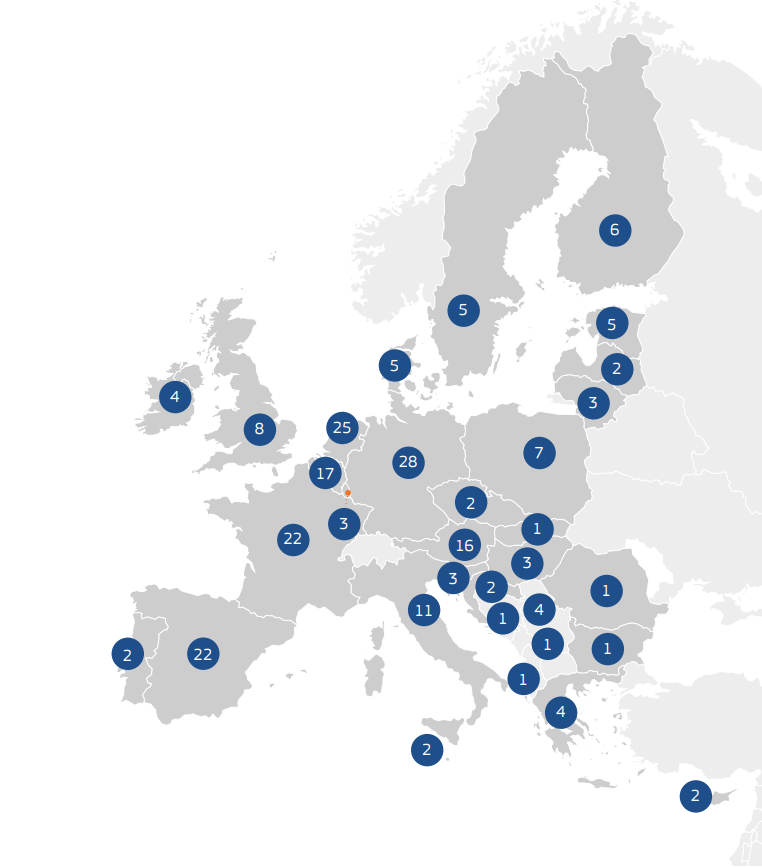
\includegraphics[width=0.6\linewidth]{Figures/01-DIHs_2018.png}
    \caption{\centering{Geographical Distribution by country of Digital Innovation Hubs in Europe as of January 2018, 2 years after the launch of the initiative. Source: \citetitle{dei2018} (\cite{dei2018})}}
    \label{fig:enter-label}
\end{figure}

\par As can be seen from the map, most of the DIHs were concentrated in central and western Europe. In fact, the country with the most DIHs is Germany, with 28 hubs, closely followed by the Netherlands with 25, France and Spain, both with 22 DIHs, and then Belgium with 17. However, if we account for the difference in population sizes, we can see how one region (apart from the Benelux block) is over-represented in terms of DIHs: the Baltics. In fact, Estonia has 5 hubs, Latvia has 2 and Lithuania has 3. Considering they have a combined population of around 7.5 million people, their 10 hubs represented a much higher concentration of hubs than other countries in Europe. For example, Italy has 8 times the population of the Baltic states, while having only 1 additional DIH\footnote{We will see in the next chapters how the high level of penetration of the DIH initiative in the baltic region will have a positive effect on the relative number of EDIHs coming from the region, as well as their productivity in terms of services provided to SMEs so far.}.


\par It's clear from the brief description provided before that DIHs were not sufficient to face the challenges of digitalization in the European private sector. Although effective at providing regional support, DIHs struggled to extend their services across regional boundaries, let alone the confines of individual member states. These shortcomings were the main reasons leading to the birth of the EDIH network, to better and improve the effectiveness of Europe's digitalization programme.

\section{The birth of the EDIH Network}

\par As part of the European Commission's \citetitle{digital_europe_programme} (\cite{digital_europe_programme}), it was decided to create a network of European Digital Innovation Hubs (EDIHs, for short). The main aim of the network was to overcome the shortcomings of the DIH Initiative. In fact, the main differences from DIHs to EDIHs are:
\begin{itemize}
    \item DIHs' funding is at the regional or national level. In fact, funding for DIHs was idiosynchratic to the specific regional or national authority to which it was dependent on. On the other hand, the EDIHs' financing comes directly from the EU budget for digitalization, and constitutes 50\% of the overall funding of each hub, with the remaining 50\% coming from regional or national funds\footnote{This could lead the reader to believe that the idiosynchratic element is still present even in the EDIH network. However, the difference with the EDIH funding is that, even if coming from regional or national budgets, the rules and regulation in place are still set by the EU regulation on the EDIHs. Thus, the degree of standardization across EU Member States is much more advanced in the EDIH than it was for the former DIH initiative}.
    \item While DIHs were for the most part operating exclusively for one specific region in which they were headquartered, the EDIHs are designed to work as a network. This means that, in theory, one firm requesting support in Portugal could be directed by the Portuguese EDIH to a different hub in Spain for example, if the Portuguese EDIH does not have the expertise needed for that specific sector.
    \item Furthermore, single EDIHs can benefit from the network by sharing best practices, expertise and know-how in order to level regional disparities across Europe. One example can be that an EDIH located in Estonia that helps firms to digitalize could share best practices with hubs in Bulgaria for example, a country that has much less experience with digitalization of the private and public sector compared to Estonia.
\end{itemize}

\par Each EDIH would be structured as a consortium of different entities, such as private companies, Higher Education Institutions, Research Centres and Public Organizations\footnote{Composition of the average EDIH will be covered in the Descriptive Statistics Section of this Chapter}. It is possible to have EDIHs with member entities belonging to different Member States of the EU. Thus, the EDIH network is not only a network of hubs, but also a network of networks, with each hub acting as a node in the network.

\section{Objectives and functioning of the EDIHs}

\par As partially covered previously, the EDIH initiative aim to fulfil the following objectives\footnote{As stated by the European Commission in the Digital Europe Programme (\cite{digital_europe_programme} and \cite{digital_europe_edih_wp_2021_2023})}:
\begin{enumerate}
    \item \textbf{Support the Twin Transition:} by providing services to support the digital and environmental transition of SMEs and PSOs.
    \item \textbf{Act as Access Points to the whole network:} single EDIHs should direct firms to the most suitable hub for their needs, even if that hub is located in a different Member State. This objective aims at addressing the limitations of the DIH initiative. 
    \item \textbf{Networking and Knowledge Sharing:} EDIHs should share best practices, expertise and know-how amongst themselves, in order to level regional disparities across Europe.
    \item \textbf{Brokering Role:} EDIHs may also act as brokers between public administrations and companies providing e-government technologies.
    \item \textbf{Experimentation and Testing:} EDIHs should provide firms with the opportunity to test new technologies before investing in them, by making available testing facilities and expertise.
    \item \textbf{Digital Capacities Multiplier:} EDIHs will act as a multiplier and widely diffuse the use of all the digital capacities built
    up under the different specific objectives of the Digital Europe Programme on High Performance
    Computing, Artificial Intelligence, Cybersecurity, Advanced Digital Skills and Accelerating the best use
    of technologies. To achieve this, EDIHs will participate in a "Train the Trainer programme", where specialist in these digital capacities will train the EDIHs on how to use them.
    \item \textbf{Interface for European Commission Policies:} EDIHs will be the interface between the European Commission and the firms, providing feedback on the effectiveness of the policies and the needs of the firms in the specific sectors they operate in.
\end{enumerate}

\par The allocation of the over 320 million euros budgeted for the EDIH initiative is done through a competitive process, where each EDIH (after having obtained the endorsment of one Member State) has to submit a proposal to the European Commission. The proposals are then evaluated by a panel of experts, and the best ones are selected to receive funding, which is then disbursed in the form of grants, covering the functioning of the hub. More specifically, all the proposals that pass the evaluation are considered eligible for funding, and are then ranked and given funding according to availability. If a proposed EDIH is deemed eligible but no funding is available, it will receive the Seal of Excellence certification: it will then be a full member of the EDIH network, but the funding for its operation will have to come entirely from regional or national funds.

\par To evaluate the performance of individual EDIHs, the Commission will rely on a set of results indicators, such as:
\begin{itemize}
    \item Number of SMEs and PSOs that accessed the EDIH's services
    \item Amount of additional investments successfully triggered by the EDIH's intervention
    \item Number of collaboration with other EDIHs and stakeholders outside the region (this indicator addresses the network dimenstion of the EDIH initiative)
\end{itemize}
\par Furthermore, some additional impact indicators will be collected and analysed by the Digital Tansformation Accelerator and the Joint Research Centre of the European Commission. These will be:
\begin{itemize}
    \item The market maturity and market creation potential of innovations, as measured by the JRC's Innovation Radar methodology.
    \item The increase in the level of Digital Maturity of ofrganization supported by the EDIHs, as measured by the Digital Maturity Assessment Tool (DMA) developed by the JRC\footnote{The design, structure and analysis of survey results from the DMA will be covered in the next chapter}.
\end{itemize}

\section{Descriptive statistics on the EDIHs}

\par As of today, the number of EDIHs operating across the EU's 27 member states is 151; however, when accounting also for Seal of Excellence Hubs, the number climbs up to 227 individual members of the network.

\par The map reported in Figure \ref{fig:edih-soe-location-map} shows the geographical distribution of EDIHs and Seal of Excellence Hubs across Europe. Addresses of the hubs were retrieved from the EDIH Catalogue, while the geocoding process was performed following the procedure that will be described in Chapter 5. 

\begin{figure}[h]
    \centering
    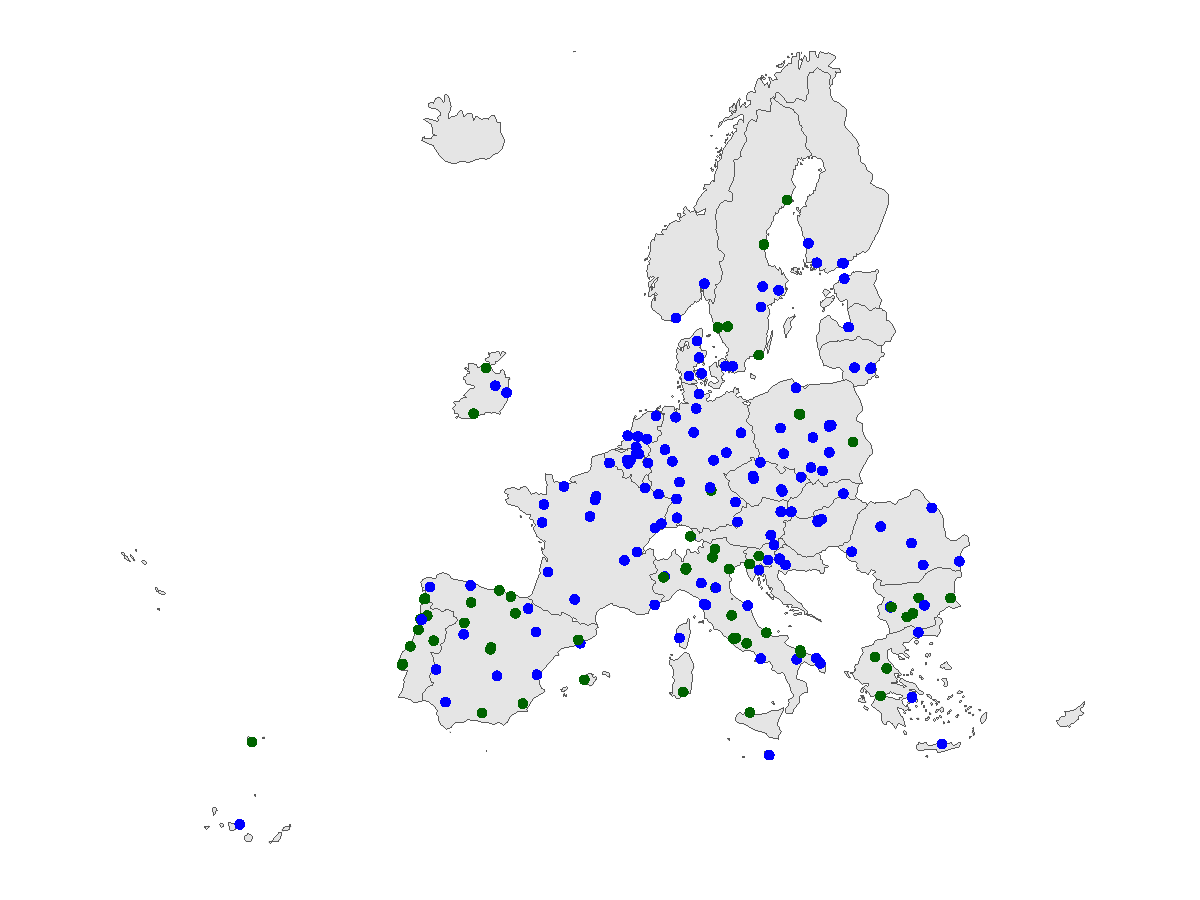
\includegraphics[width=1\linewidth]{../Output/EDIH_and_Seal_of_Excellence_map.pdf}
    \caption{\centering{Geographical Distribution of European Digital Innovation Hubs (blue dots) and Seal of Excellence Hubs (green dots) in Europe as of March 2024. Source: Author's elaboration based on the geocoding of hubs in the EDIH Catalogue}}
    \label{fig:edih-soe-location-map}
\end{figure}

\par The map shows a clear concentration of hubs in central and western Europe, with a lower number of hubs in the eastern and southern regions. This is in line with the distribution of DIHs, as shown in Figure \ref{fig:enter-label}. The Baltic region, however, is still over-represented, with 4 EDIHs and no Seal of Excellence Hubs. We will see in the next chapters how this will impact the number of firms in the sample that have interacted with the Baltic EDIHs.

\par It is easy to note that most of the Seal of Excellence hubs are located in the Southern and Eastern regions of the EU. This means that, while a lot of proposed hubs in these regions were deemed substantially worthy to be considered eligible, their proposals were considered less effective than those of the hubs that received funding. This could potentially have an impact on the effetiveness of the initiative in these particular regions, it the hubs do not manage to secure the necessary funding from national or regional budgets.

\par The JRC's report (\cite{jrc_edihreport}) also provides some data on the current state of the EDIH network. On the regional distribution, it stresses the success of the reported regional coverage of EDIHs, stating that EDIH services are available in 223 regions, roughly 90\% of the NUTS2 regions making up the EU. Furthermore, 213 regions host at least one organization that participates in the EDIH network. 

\par Looking at the composition of the EDIHs from the table in Figure \ref{fig:edih-composition-table}, we see that the average EDIH is composed of 11 participants, with 3 of them being Private Companies, 2 being Higher Education Institutions, 2 being Research Centres and another 2 being Public Organizations. An average of 3 participants per EDIH are labeled as "Other". This composition underlines a somewhat strong presence of the private sector in the EDIH network, which is in line with the objective of the initiative to foster public-private partnerships. The total number of participant entities in the EDIH network is 2355 unique organizations as of the writing ot the JRC Report on the EDIH network.

\begin{figure}[h]
    \centering
    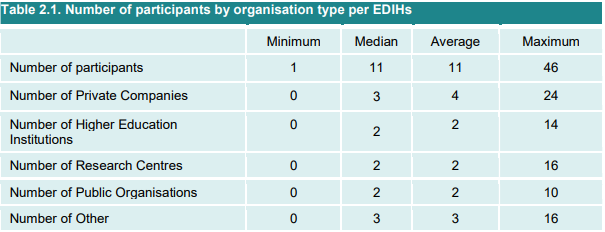
\includegraphics[width=1\linewidth]{Figures/05-edihcomposition.png}
    \caption{\centering{Data on composition of the EDIHs. Source: \cite{jrc_edihreport}}}
    \label{fig:edih-composition-table}
\end{figure}

\par The report also shows how the participating entities in the EDIHs primarily come from the NACE sector related to Professional, Scientific and Technical Activities, as well as Education and Information and Communication. This is consistent with the focus of the program on upskilling and digitalization of firms.

\par As far as technological targeting goes, the most targeted technologies are AI (91\% of EDIHs), Cybersecurity (70\%) and Internet of Things (64\%). This reflects well on the  adherence of the EDIH network to the stated objectives of the Digital Europe Programme, since these are some of the technologies specifically cited as a focus of the programme itself.

\par The most targeted sectors by the EDIHs are instead Manufacturing (64\%)\footnote{This will be reflected in the DMA survey responses, as well as in the overall analysis on the drivers of participation in the EDIH initiative}, Health Care (47\%) and Public Sector (44\%). Out of the services the EDIHs can provide, the most widely offered are SME support (81\%), Ecosystem building (72\%) and Technological Innovation (71\%).

\par Note however that all these data are based on self-reporting by individual EDIHs at the start of their operation, so they should be taken with a certain amount of skepticism. Fortunately, by now we have reporting data on actual services that were performed by the EDIHs, so it is possible to directly check the veridicity of the self-reported data. The analysis on the sectors in which supported firms operate, as well as the techologies covered, will be partially covered in the next chapters. Here I will present only a quick rundown on the nature of services provided by the EDIHs so far, as well as a snapshot of the sectors supported by EDIHs\footnote{The attentive reader will note that the number of reported services does not match the number of respondents to the DMA survey that will be reported in the next chapter. This is due to a variety of reasons, but the main one is related to the timing mismatch between the reporting of the services delivered by EDIHs and the submission of the survey to the DTA. It is often the case that the service gets delivered and then some weeks or even a month pass before the survey is loaded on the platform.}.

\begin{figure}[h]
    \centering
    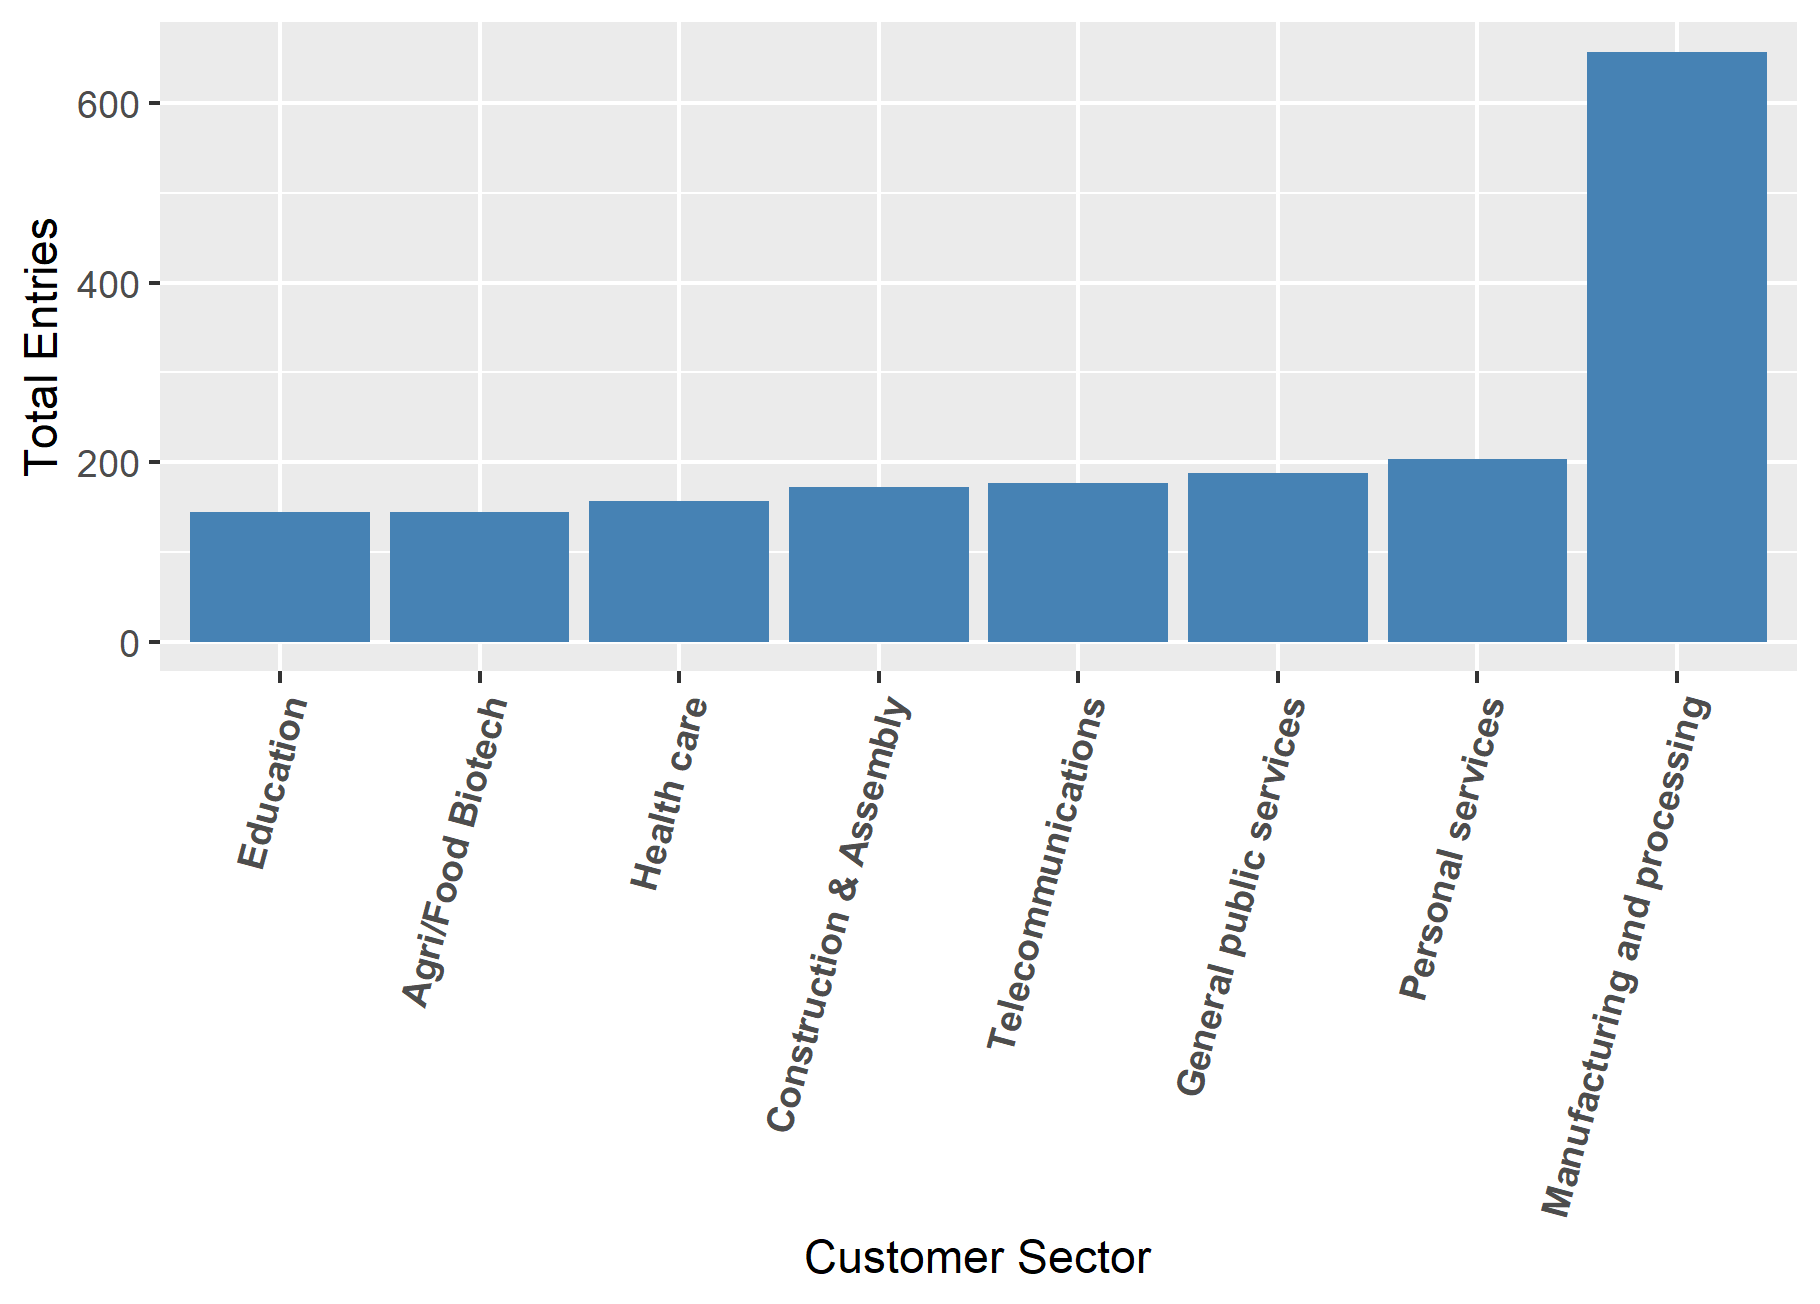
\includegraphics[width=0.8\linewidth]{../Output/cust_sector_plot.png}
    \caption{\centering{Data on sectoral composition of the EDIHs customers (for the sake of readability, only sectors with more than 125 entries are reported).}}
    \label{fig:edih-customersector-table}
\end{figure}

\par Looking first at the sectoral snapshot of supported firms and PSOs, we can see that by far the most represented sector is Manufacturing and Processing, which constitutes more than 600 entries in the reporting dataset. Just after that, Personal Services comes as a striking second place, considering that it was never explicitly targeted by EDIHs. It is then followed closely by General Public Services (reflecting the presence of PSOs in the dataset), and then by Telecommunication, Construction and Assembly, Health Care, Biotech and Education. We can see that there is a partial overlap between the sectors most targeted by EDIHs and those where their customers operate, but the overlap is not perfect. For example, Biotech and Personal Services were not explicitly targeted by a large number of EDIHs (only 29\% and 11\% of EDIHs respectively), yet they are among the most represented sectors in the dataset.


\par In the next bar chart we can see some data on the type of services provided so far by EDIHs. The most common service reported is "Networking and access to innovation ecosystem"; this is the category that encompasses all services that help EDIH customers in connecting with potential partners, becoming part of innovation clusters, or organizing networking events. Seeing this service category as the most common can be a good sign, since this is the category that most benefits from the network dimension of the EDIH initiative. Next is the "Test before invest" category, which includes all types of prototyping or technology testing services that the EDIHs offer. "Training and skills development" is a close third, signaling the importance of upskilling in the digitalization process. Lastly, "Support to find investment" is the least popular service category, which could be a sign that the EDIHs are not yet fully exploiting their potential as brokers between firms and investors.

\begin{figure}[h]
    \centering
    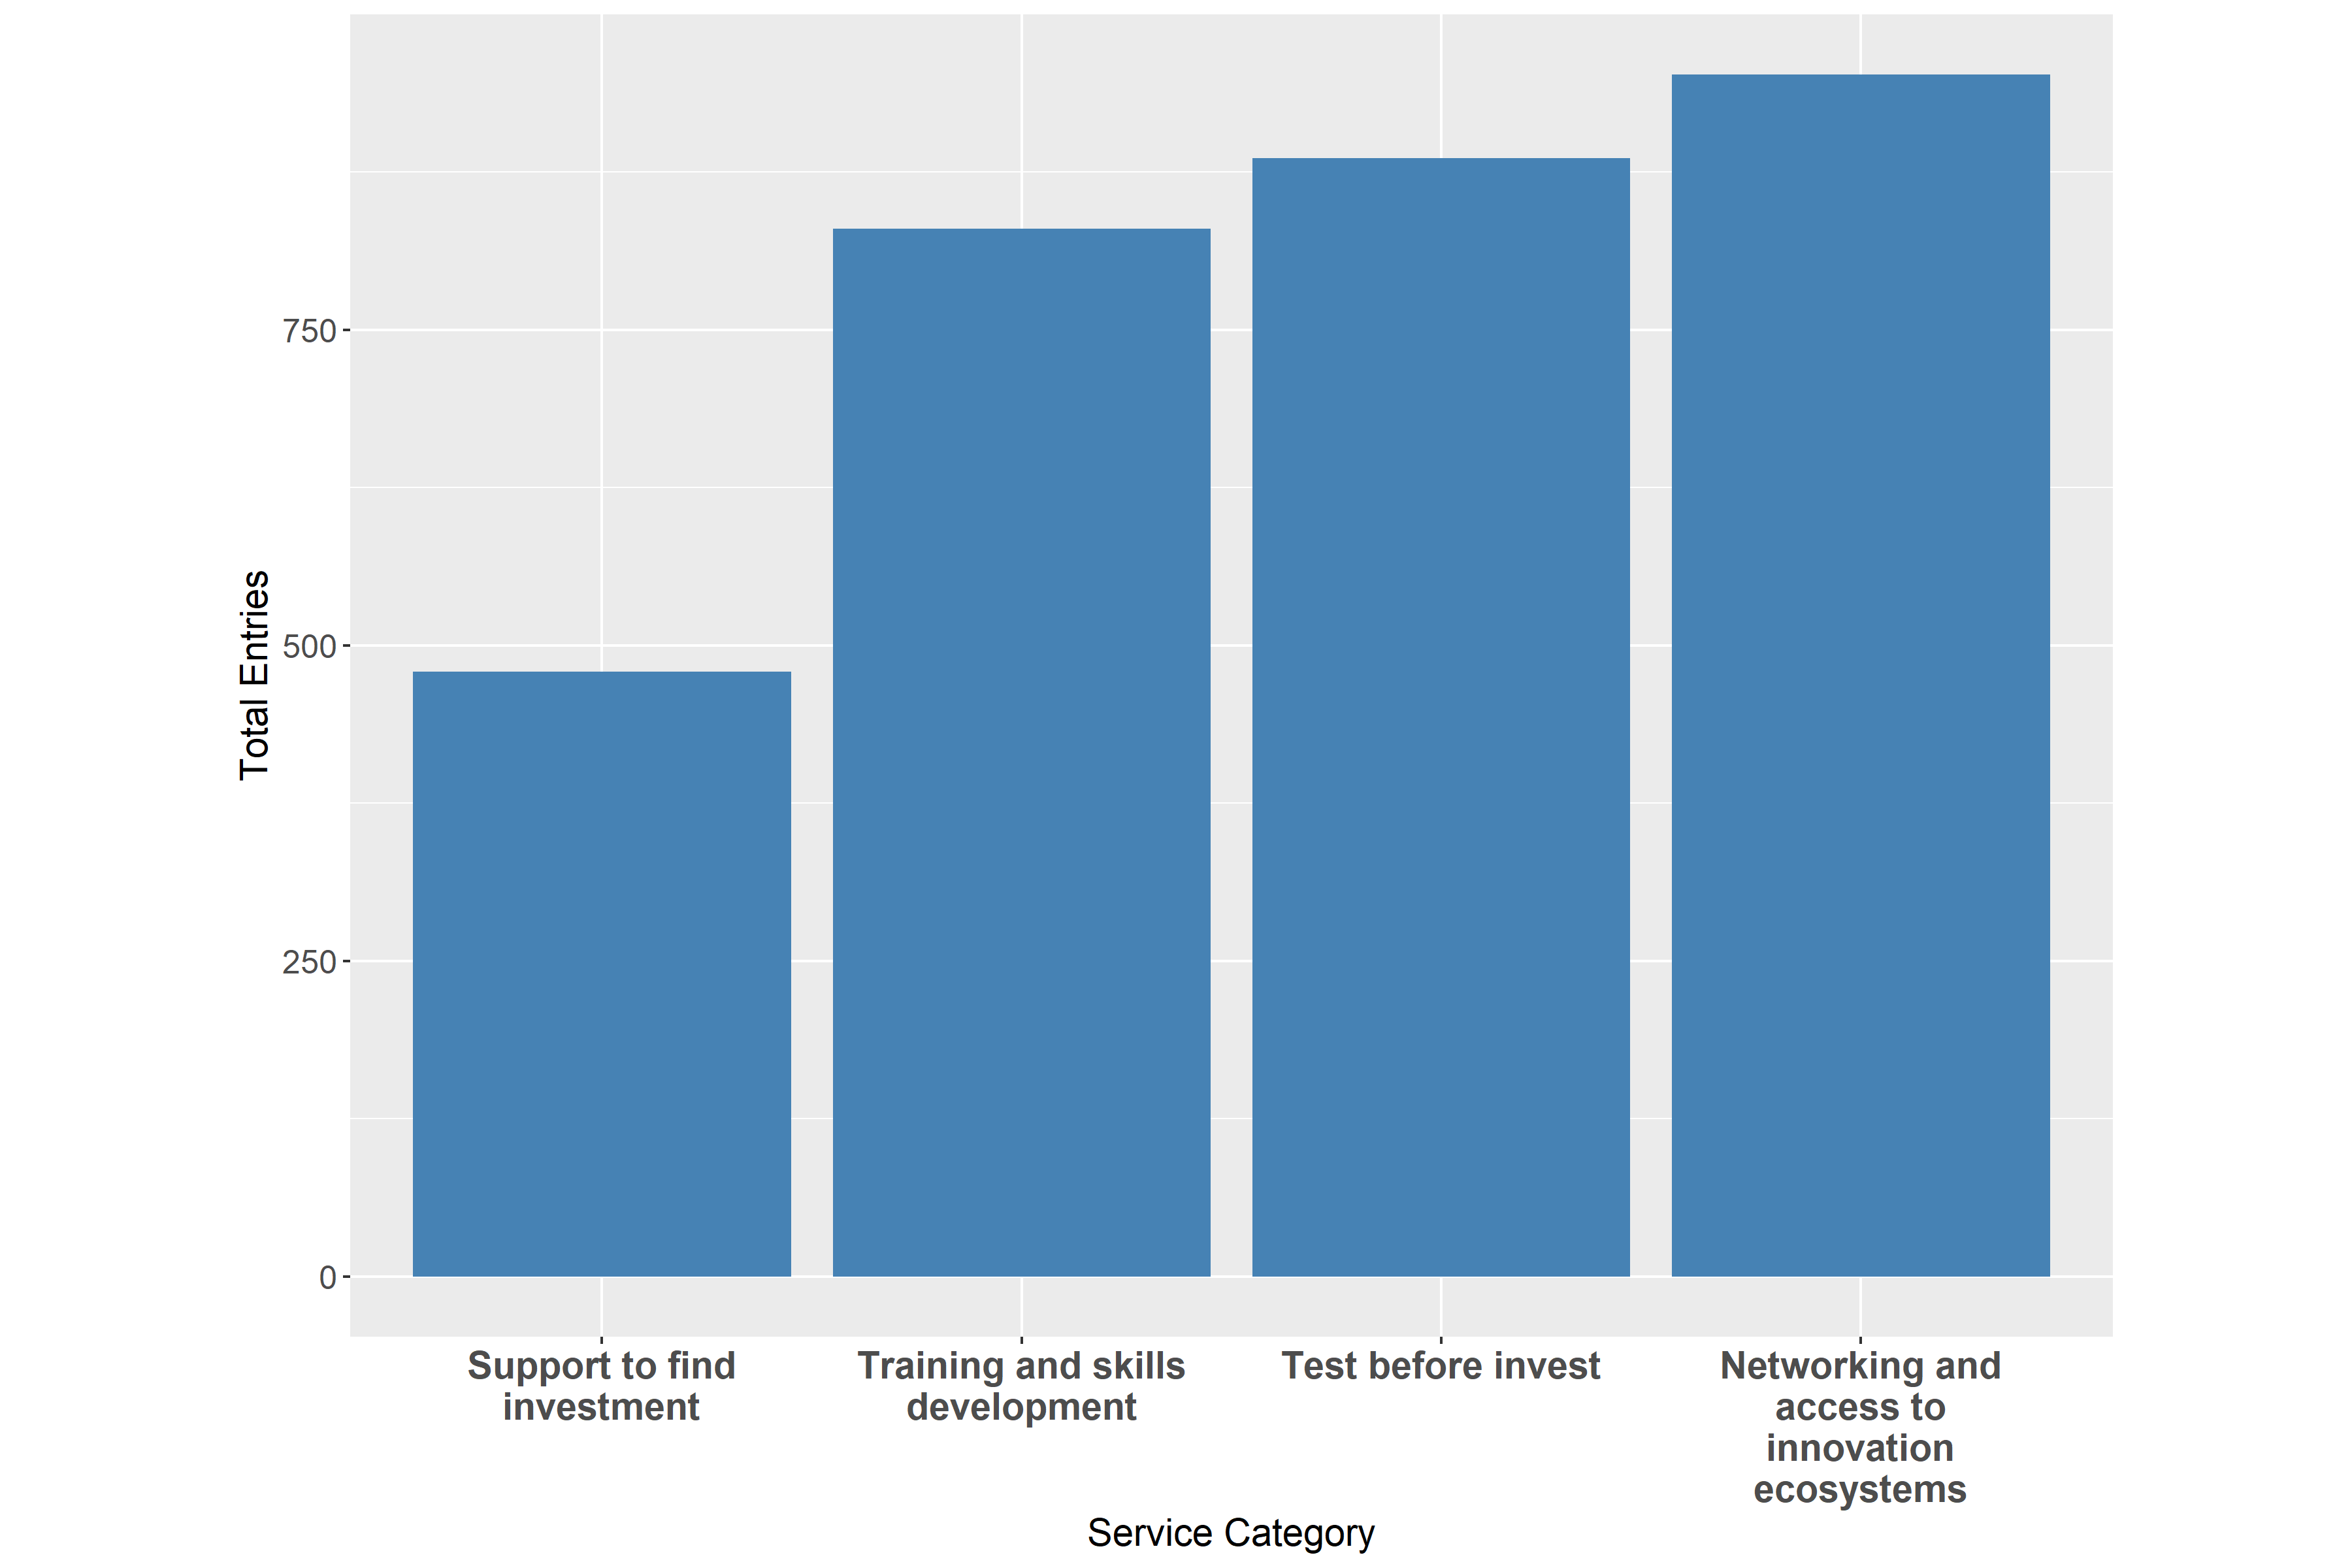
\includegraphics[width=1\linewidth]{../Output/service_categ_plot.png}
    \caption{\centering{Data on the distribution of services provided by the EDIHs. }}
    \label{fig:edih-services-table}
\end{figure}






\newpage
\chapter{The DMA Survey}

\par While the EDIH network was being formed, the European Commission's DG CNECT decided it needed result and impact indicators to evaluate the performance of individual EDIHs, as well as the overall initiative. 
\par Thus, in addition to result indicators to be reported by the individual EDIHs, DG CNECT delegated the JRC to design and validate an assessment questionnaire for measuring the digital maturity of EDIH customers (SMEs).
\par The validation was performed by testing the survey on a sample of SMEs around Europe and with the already active DIH community, precursor of the EDIH network.
\par In a second phase, an assessment survey was designed also for Public Sector Organization (PSOs); however, due to our focus on the part of the EDIH initiative that deals with private sector firm, I am not going to cover that version of the survey here.

\par I will now go over the design process and the overall structure of the survey, and then proceed to present some analysis of the survey responses obtained so far, from the sample of firms that I will then use for the main analysis.


\section{Design and structure of the survey}

\par The rationale behind the creation of a new DMA framework to be used by EDIHs is that measuring the level of digital maturity of a firm and its evolution over time will provide a useful indication of the effectiveness of the intervention, and at an aggregated level, it will be possible to assess the effectiveness of the EDIH policy initiative.

\par Thus, the Digital Maturity Assessment Survey (DMA) was designed to investigate the base digital maturity level of the firm receiving support from the EDIH, before the intervention starts. The survey was then to be submitted two more times: the first one set for 1 year after the initial DMA submission, and the second one 2 years after the first one\footnote{Specifically, according to \cite{jrc_dmamanual}, we have the following definitions:
\begin{itemize}
   \item $T0$ = before EDIH intervention (a point in time no longer than 6 months prior to EDIH support)
   \item $T1$ = 1 year after T0 (if EDIH intervention still running, wait until it is concluded. It should be applied not later than 3 months after EDIH support has been delivered.)
   \item $T2$ = 2 years after T1 (a further point in time no earlier than 18 months and not longer than 24 months after EDIH suppor has been delivered)   
\end{itemize}}.

\begin{figure}[ht]
    \centering
    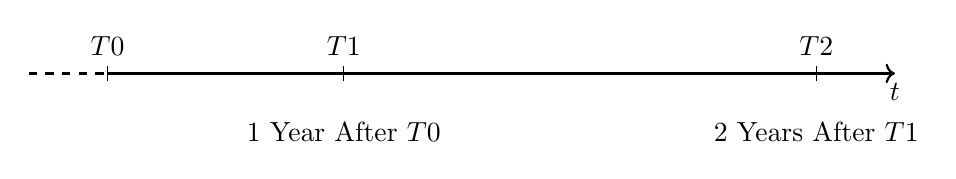
\begin{tikzpicture}
        % Draw the timeline arrow with dashed line at the beginning
        \draw[dashed, thick] (0,0) -- (1,0);
        \draw[->, thick] (1,0) -- (11,0) node[anchor=north] {$t$};

        % Draw the points t0, t1, t2 at mid height
        \foreach \x/\label in {1/$T0$, 4/$T1$, 10/$T2$} {
            \draw (\x,-0.1) -- (\x,0.1) node[anchor=south] {\label};
        }

        % Optional: Add labels below the timeline
        \node[anchor=north] at (1,-0.5) { };
        \node[anchor=north] at (4,-0.5) {1 Year After $T0$};
        \node[anchor=north] at (10,-0.5) {2 Years After $T1$};
    \end{tikzpicture}
    \caption{Timeline of DMA Submissions}
    \label{fig:timeline}
\end{figure}

\par The survey itself was organized in two main modules:
\begin{enumerate}
    \item Module 1: Customer Data
    \item Module 2: Digital Maturity for SMEs
\end{enumerate}

\par The first module contained basic data to identify the firm, as well as some statistical filters, such as:
\begin{itemize}
    \item Enterprise identification
    \item Contact information (Address, Email, etc.)\footnote{Address information to geocode  treated firms was taken from here}
    \item Staff size
    \item Foundation year
    \item Special SME categories
    \item Country/Region info (NUTS2, ZIP code)
    \item Sector of axctivity (NACE compatible)\footnote{The classification system itself is compatible with the NACE classification. However, for the purpose of easy compatibility with the ORBIS data and to more easily compare with the control group, I opted to use the NACE codes found in ORBIS instead of the classification designed by DG CNECT.}
\end{itemize}

\begin{figure}[ht]
    \centering
    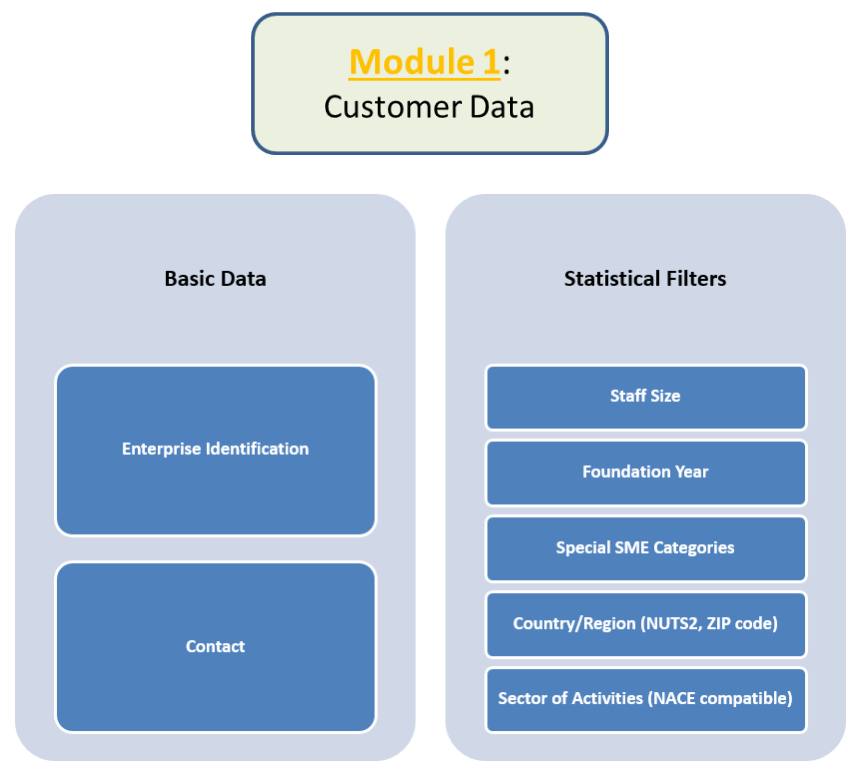
\includegraphics[width=0.9\textwidth]{Figures/02-dmamodule1structure.png}
    \caption{Structure of Module 1. Source: \cite{jrc_dmamanual}}
    \label{fig:dma_module1_survey_structure}
\end{figure}


\par The second module is the core part of the DMA questionnaire. It consists of question assessing different aspects of the digital maturity of an organization, grouped under six dimensions, which for the SMEs' survey are:

\begin{enumerate}
    \item \textbf{Digital Business Strategy:} the questions in this dimension aim to assess the overall status of the enterprise's digitalization strategy. They inquire wether the firm invested in it across various business areas (both completed and planned) and the company's preparedness to undertake a digital transformation. 
    \item \textbf{Digital Readiness:} it measures the current uptake of digital technologies (both basic and advanced ones).
    \item \textbf{Human - Centric Digitalization:} this dimension evaluates how staff are trained, involved, and empowered through digital technologies, and how their working conditions are enhanced to boost productivity and wellbeing.
    \item \textbf{Data Management:} it captures if and how data is digitally stored and made accessible throughout the organisation, as well as exploited for business purposes, while being protected via cybersecurity schemes.
    \item \textbf{Automation \& Intelligence:} it explores the level of automation and AI employed in business processes.
    \item \textbf{Green Digitalization:} measures the capacity of the firm to undertake digitalization with an approach that cares about the protection and sustaintability of natural resources and the environment.
\end{enumerate}

\par Each dimension is divided into two subdimensions (apart from Automation \& Intelligence, which has only one), as you can see from the image below.

\begin{figure}[ht]
    \centering
    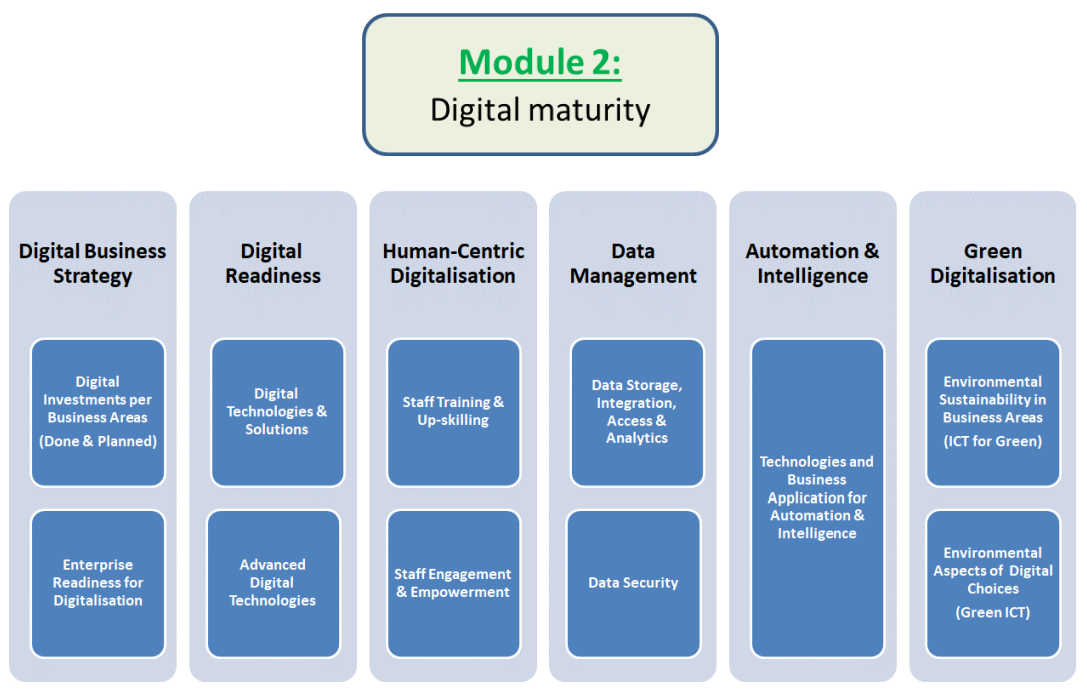
\includegraphics[width=1\textwidth]{Figures/03-dmamodule2structure.png}
    \caption{Structure of Module 2. Source: \cite{jrc_dmamanual}}
    \label{fig:dma_module2_survey_structure}
\end{figure}

\par Each of the subdimension constitute one question in the survey, with several items contained in the question. The actual number of options in each question varies from one subdimension to the other. Each dimension is scored on a scale from 0 to 100, with higher scores indicating higher maturity. The overall DMA score is then computed as a simple average of the six dimensions, and is also on a scale from  0 to 100.

\par See below an example of a question from the DMA, specifically from the Advanced Digital Technologies subdimension in the Digital Readiness dimension. As you can see, for each advanced digital technology considered, the firms can select the level at which they use that specific technology, and get a score based on that.

\begin{figure}[ht]
    \centering
    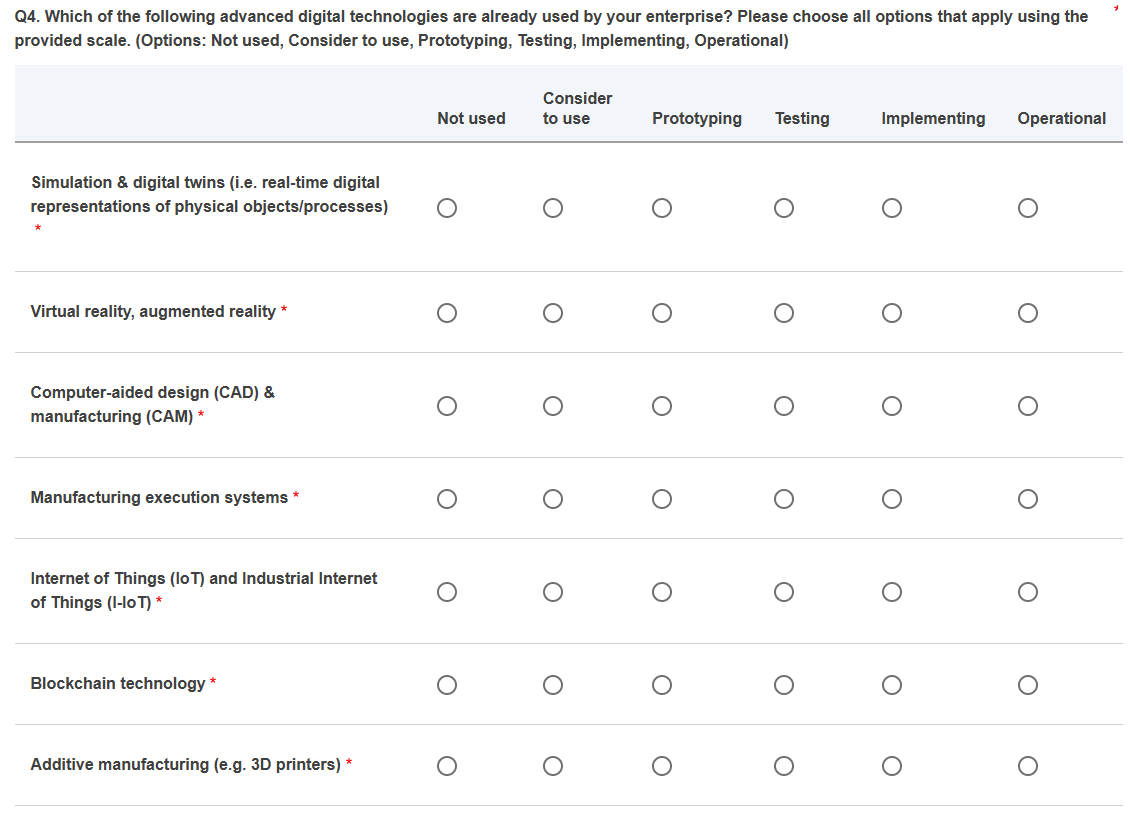
\includegraphics[width=1\textwidth]{Figures/04-dmasurveyquestionexample.png}
    \caption{Example of a question from the DMA. Source: \href{https://european-digital-innovation-hubs.ec.europa.eu/open-dma}{DMA website}}
    \label{fig:dma_survey_question}
\end{figure}

\par As an incentive for firms to complete the survey in an accurate way the DMA, upon submission the website shows the results of the assessment and how the level of the firm's digital maturity compares with peers in their area or sector.




\newpage
\section{Analysis of the survey responses}
\par Let's start with some statistics on the number of firms involved. As of the time of writing, the sample of firms that submitted the DMA consists of about 3200 entities.

\par You can see a breakdown of the firms by country of origin the bar chart below. 


\begin{figure}[h!]
    \centering
    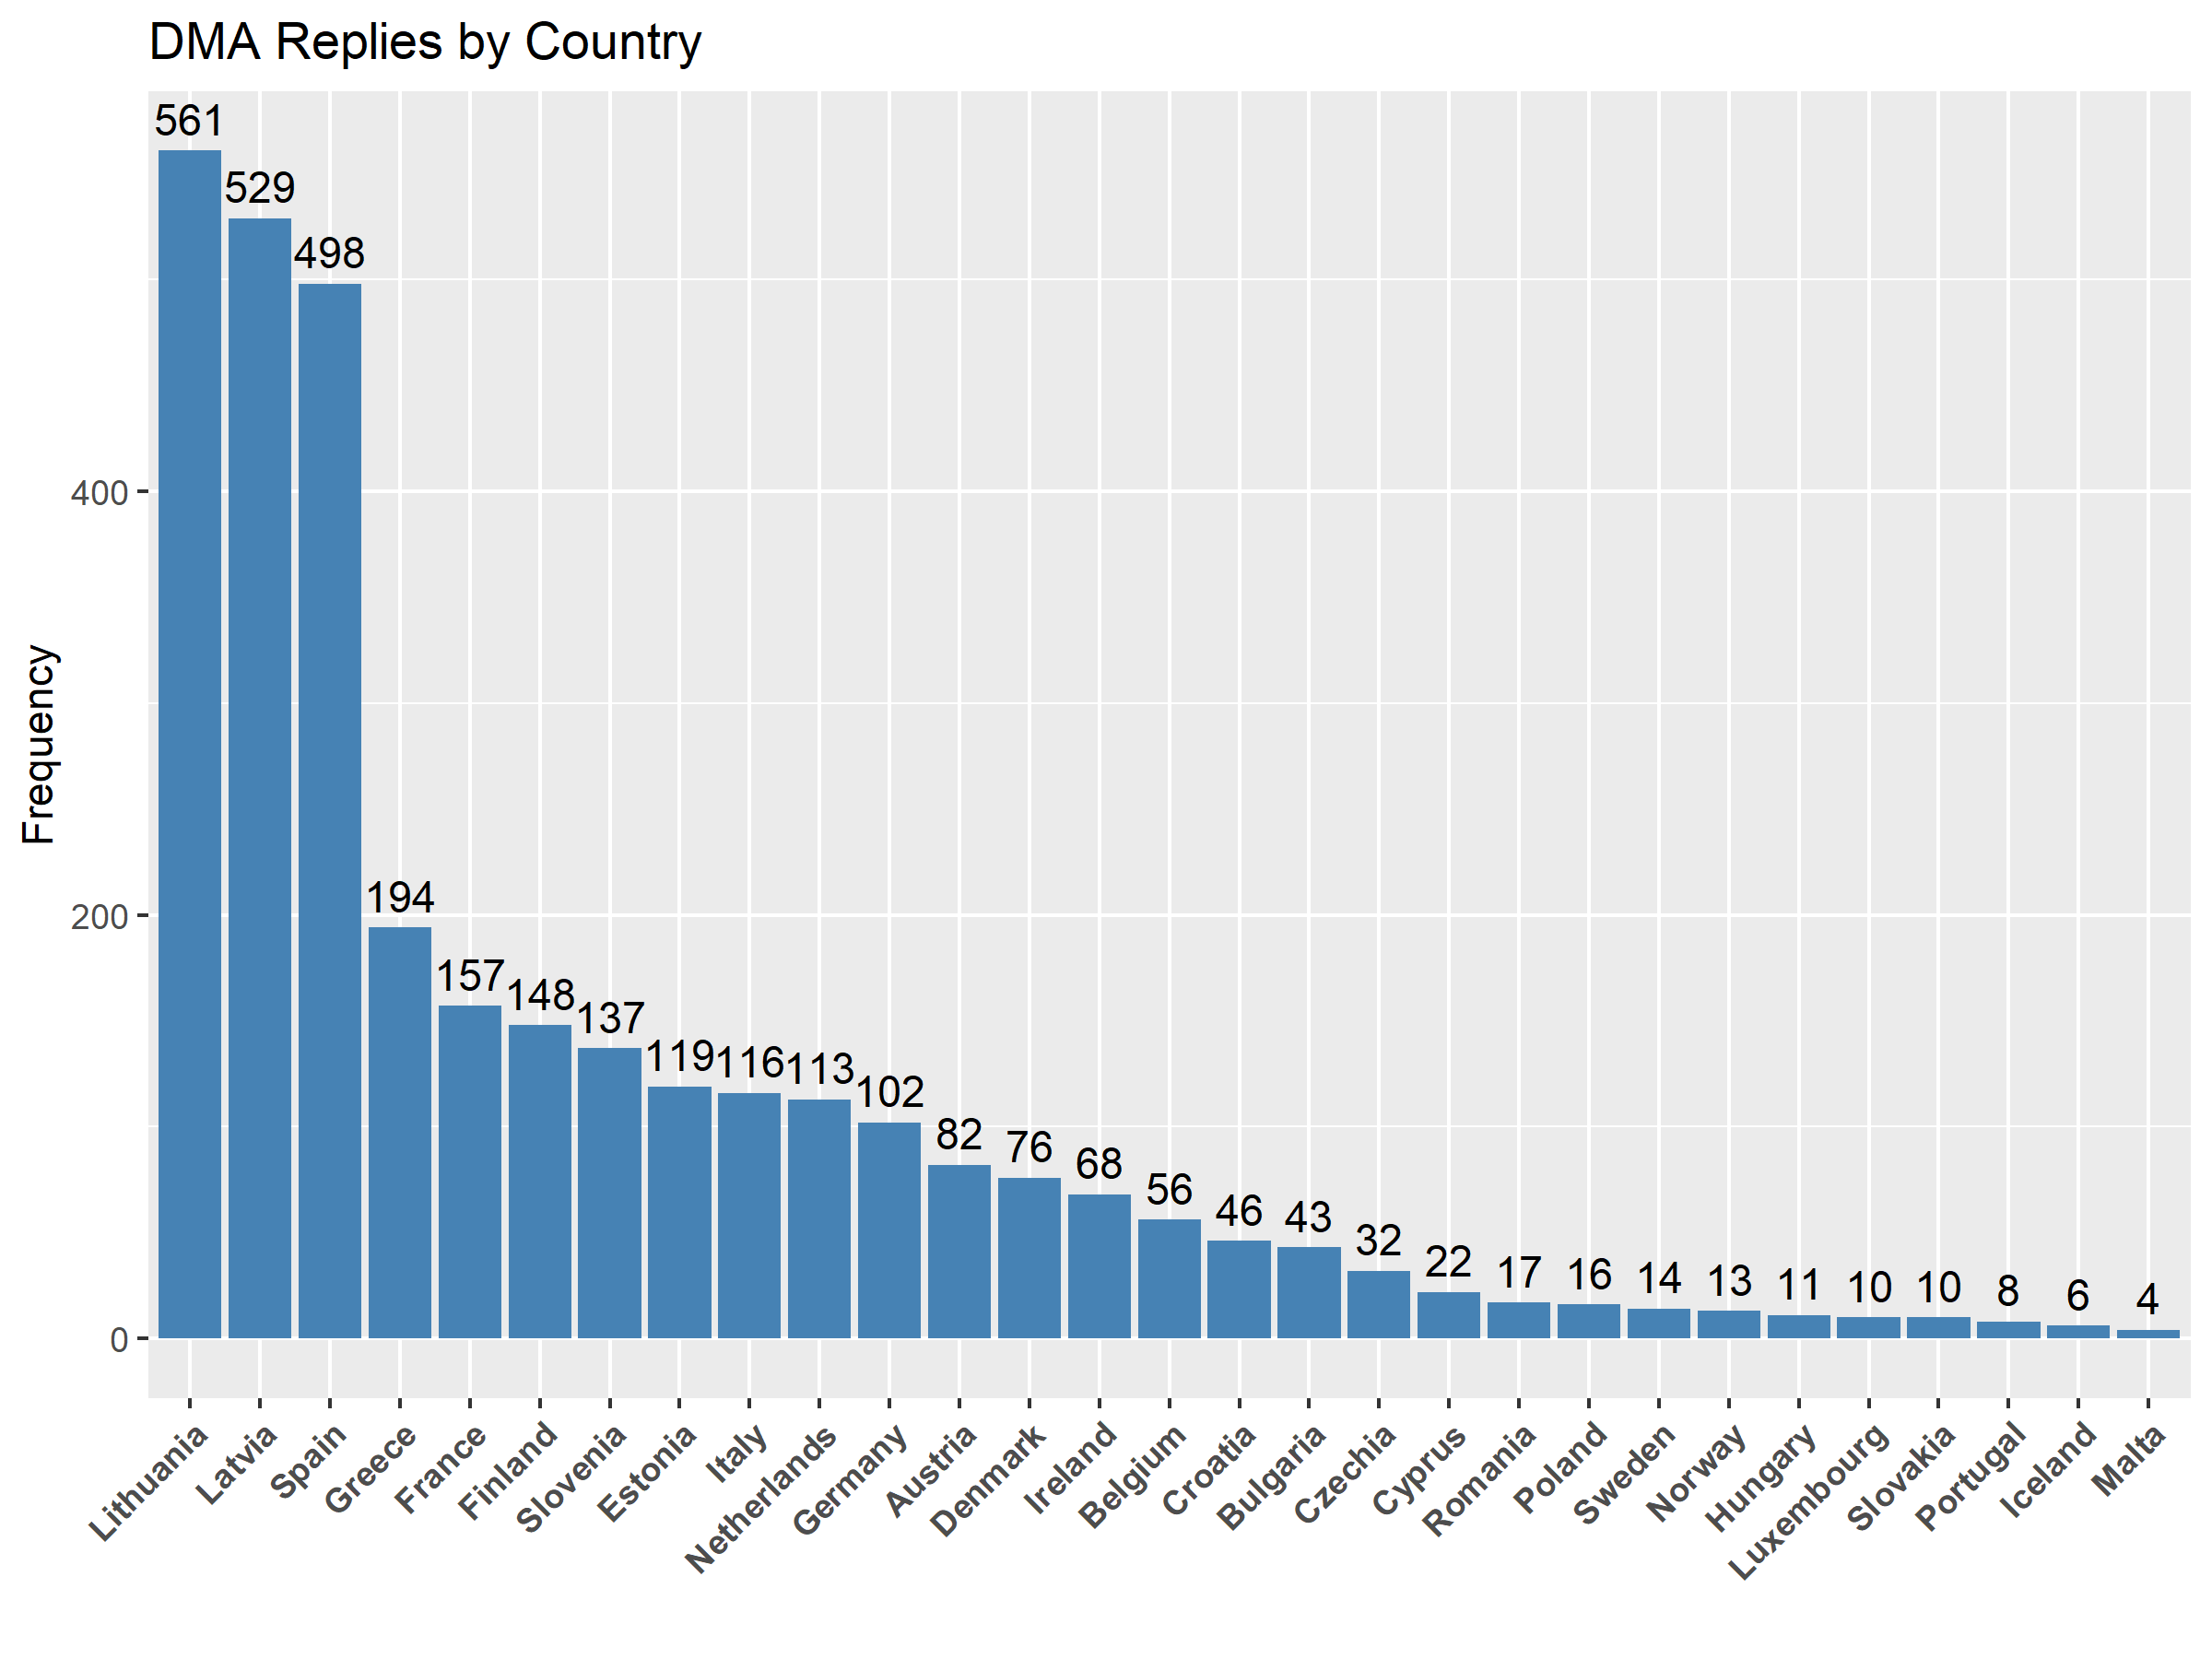
\includegraphics[width=\linewidth]{../Output/dma_country_distr_col.png}
    \caption{\centering{Distribution of DMA respondents by country of origin.}}
    \label{fig:dma_bycountry}
\end{figure}

\par It is immediately clear that the distribution of respondents is not uniform across countries. In fact, almost a majority of the respondents come from Lithuania, Latvia, or Spain. This is likely due to the fact that the DIH program was particularly successful in the Baltic countries (and in fact, even Estonia and Finland have a large representation in the sample compared to larger countries). 

\par Anyway, this would mean that the sample of firms we are observing here is not in any way representative of the overall population of firms in the EU. With regards to the geographical dimenstion, I will account for this by adding the country of origin as a control variable in the regression analysis\footnote{The original idea was to utilize country-specific fixed effects. However, the sample size for some of the countries, once having accounted for the data loss related to the matching process with ORBIS, was not enough to allow for that. Thus, I decided to include group of countries as regressors in the analysis.}.

\par We can now proceed to analyze the breakdown by firm size. The first module of the DMA survey contains information on the size of firms, since it asks the respondents to declare their number of employees. This is done through a cathegorical variable, with the following options: Micro-size (1-9), Small-size (10-49), Medium-size (50-249), Small mid-cap (250-499), Mid-cap (500-2999) and Large company (3000+). Of course, the variable is self-reported, and thus it is possible that some respondents might have misreported their size. This is the reason why, once the matching with ORBIS data was done, I decided to use the number of employees as reported in the ORBIS database, to have a more accurate measure of firm size. Nonetheless, these responses allow us to get a first look at the composition of the sample.

\begin{figure}[h!]
    \centering
    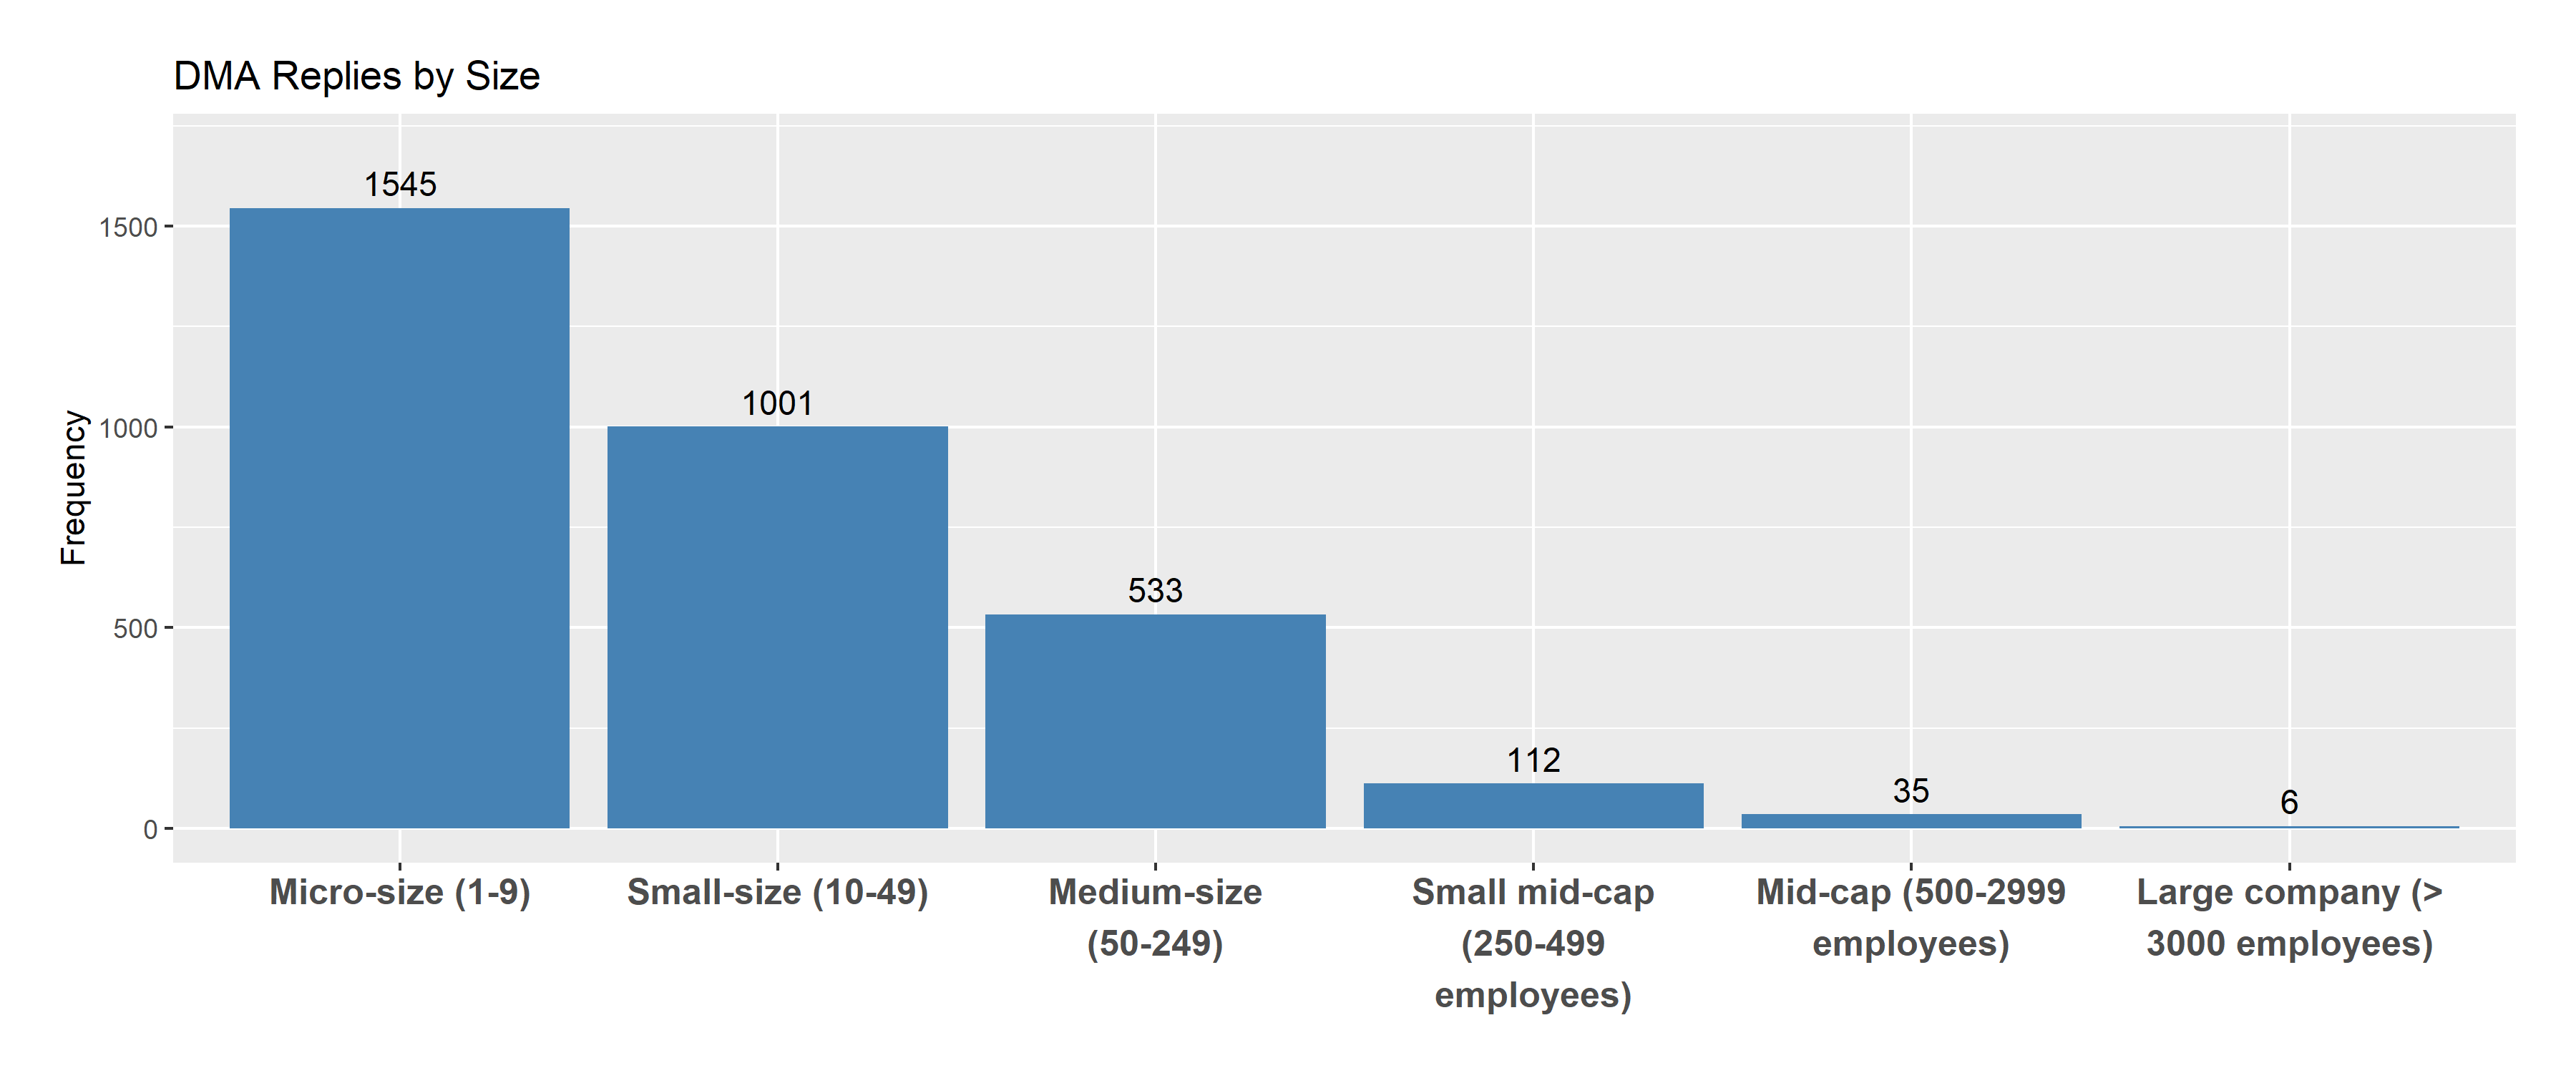
\includegraphics[width=\linewidth]{../Output/dmafirmsizebargraph.png}
    \caption{\centering{Distribution of DMA respondents by number of employees}}
    \label{fig:distr_employees}
\end{figure}

\par As we would expect, we can notice right away how almost half of the firms in the sample are micro-sized, with a number of employees between 1 and 9. Another third is classified as small-sized, with 10 to 49 employees; medium-sized firms are also well represented. This seems to confirm the aim of the EDIH initiative, which is to target small and medium-sized enterprises. As a potential future research topic, since one of the objectives of the digitalization initiative is to make european firms more competitive and help them grow, it would be interesting to see if these firms were able to grow in size.

\par In the first module of the survey, firms aso self-report their sectoral activity. This is done through a European Commission classification system, designed to be compatible with NACE classification.
\begin{figure}[h!]
    \centering
    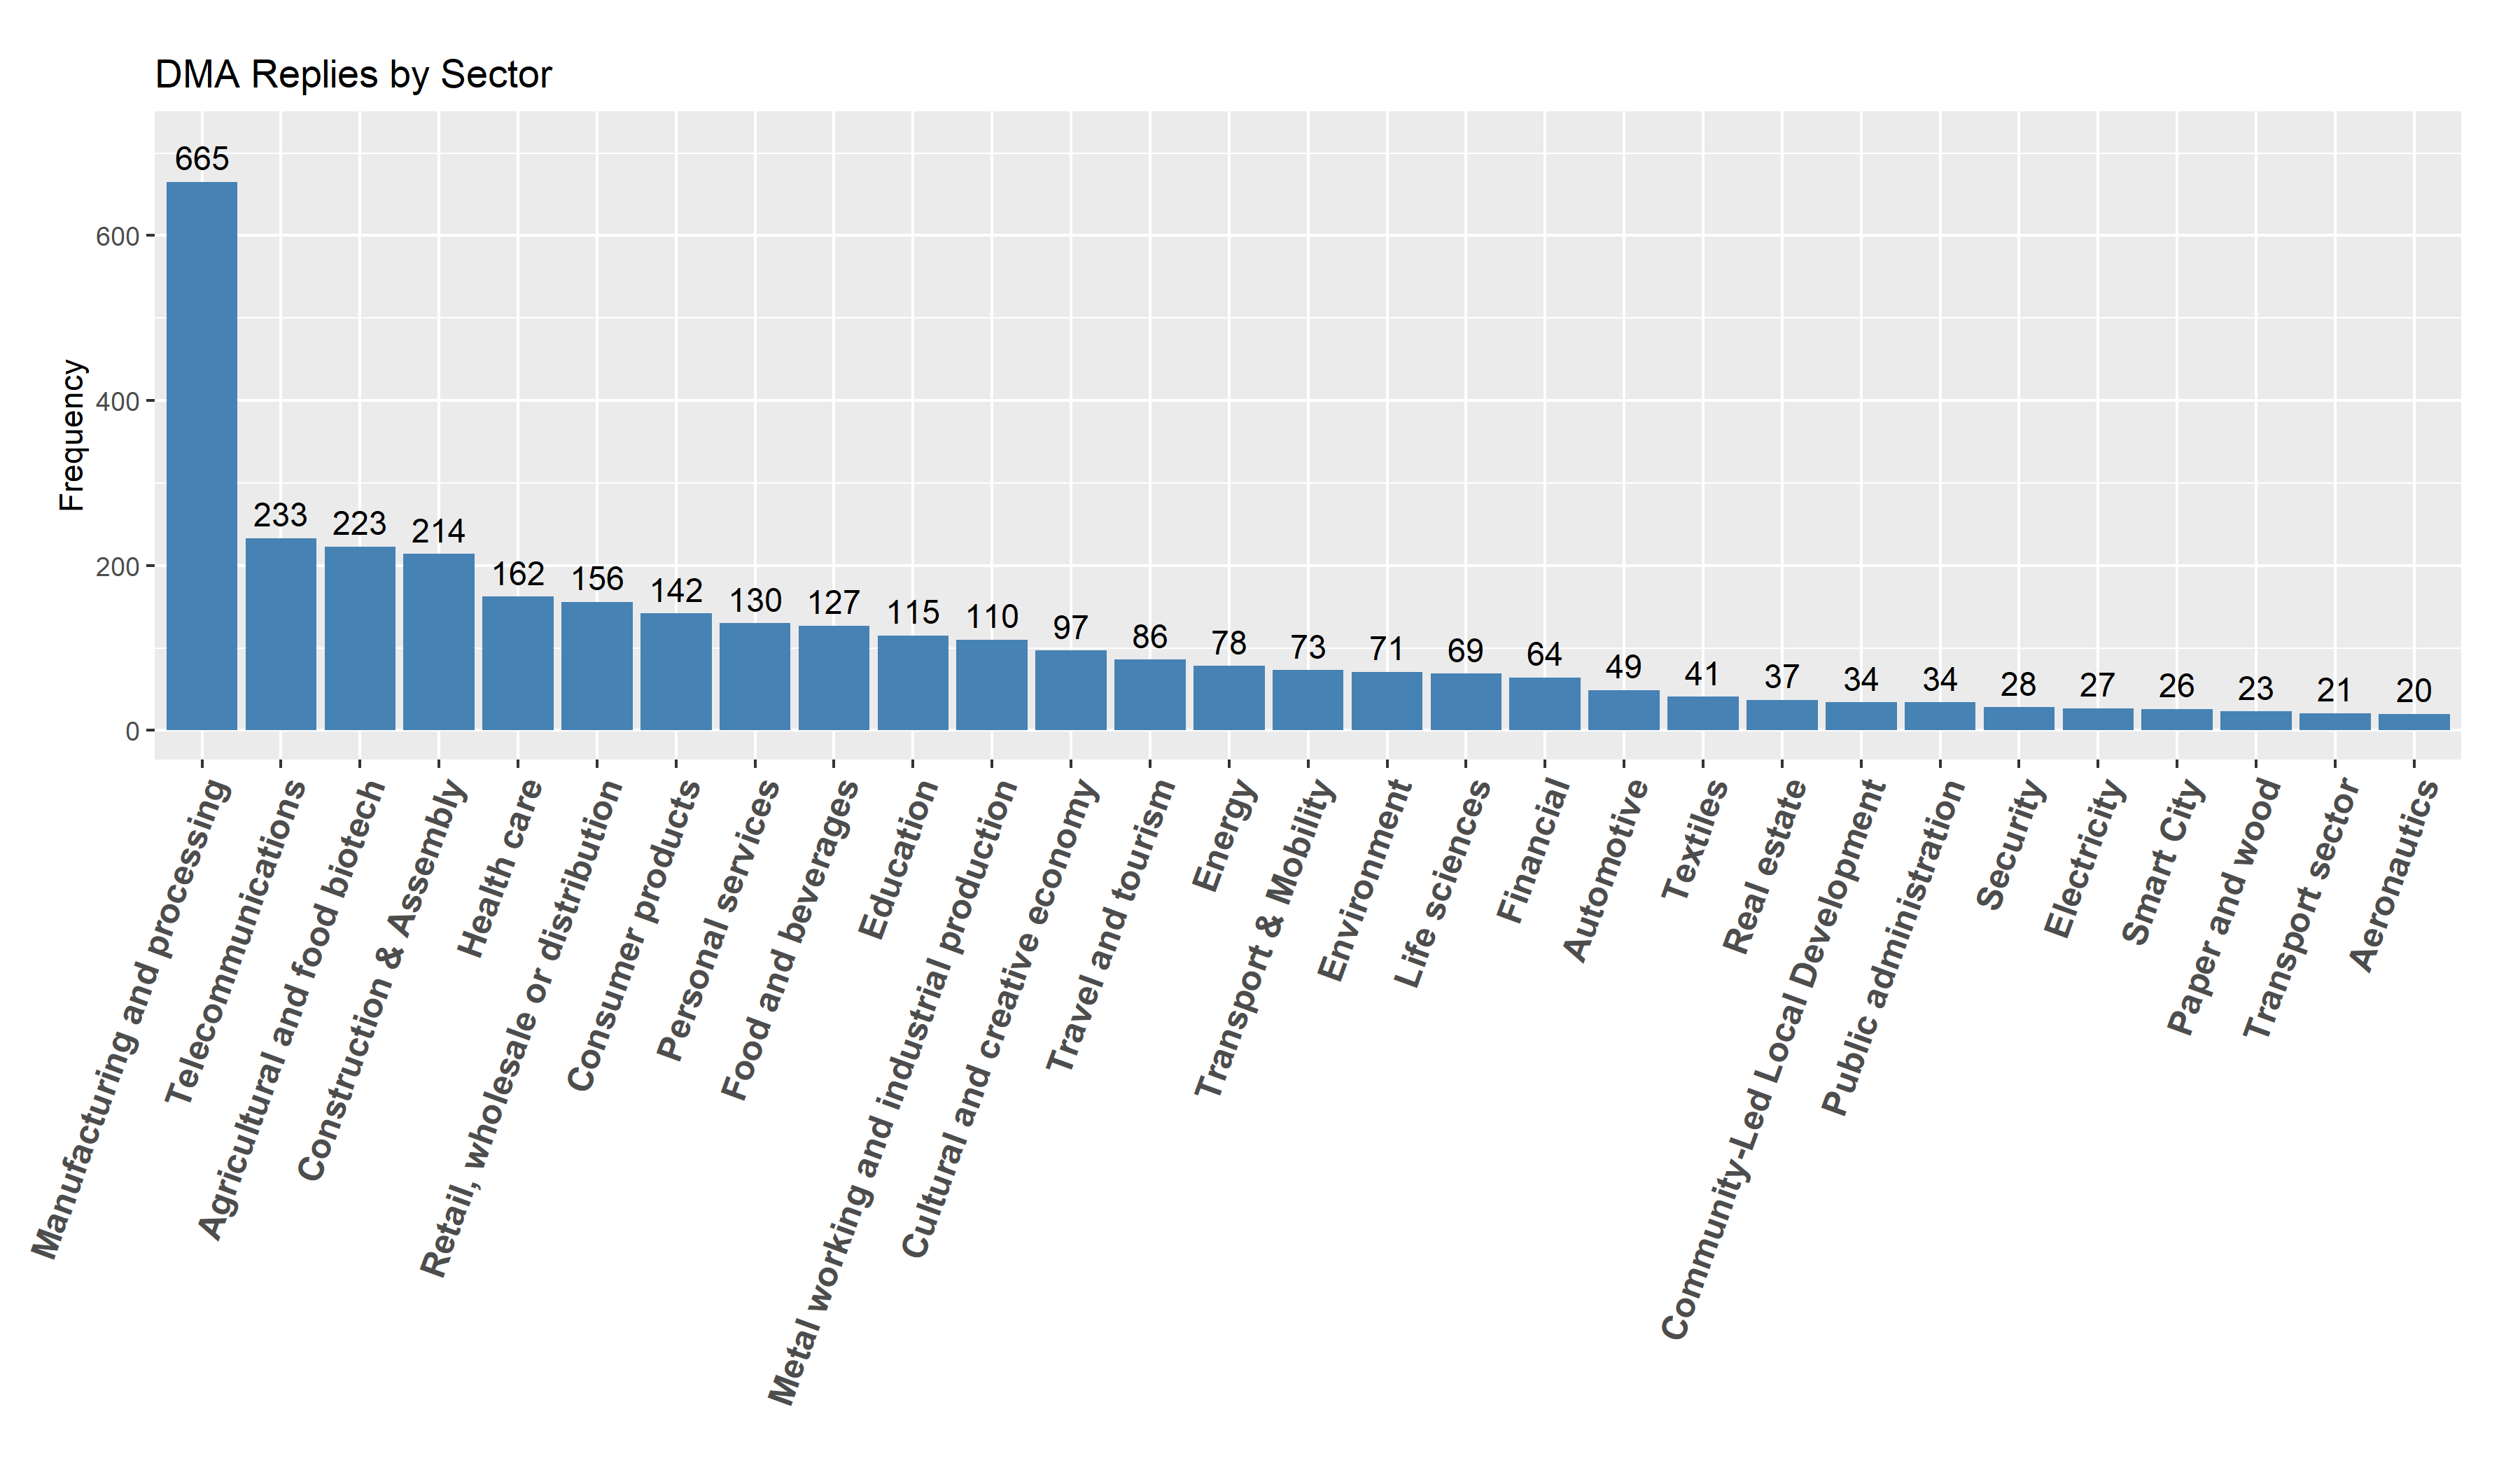
\includegraphics[width=\linewidth]{../Output/dmasectorsbargraph.png}
    \caption{\centering{Distribution of DMA respondents by sector of activity}}
    \label{fig:distr_sector}
\end{figure}

\par As we can see, a plurality of the firms surveyed are part of the Manufacturing and Processing sector. Other sizeable portions of the sample are represented by sectors such as Telecommunication, Biotechnology, and Construction and Assembly. This is to be expected, since these sectors are already characterized by being highly technologically intensive ones; thus, it makes sense they would be among the firsts to take part in the EDIH initiative.


\par Let's move to a quick overview of the replies from the DMA survey's questions. If we look at the overall score, the first thing we notice is the difference in average score and distribution between the different dimensions. We notice right away how the Automation \& Intelligence dimension represents a sginificant drop in average score compared to all the other dimensions. In fact, we can see how more than 25\% of firms present a score in that dimension that is actually equal to zero. Thus, even if the average score is around 20 points, the median is likely around 17. This suggest a serious deficiency in the uptake of innovative digital technologies, as the second-lowest average score is represented by the digital readiness dimension, which measures the uptake in specific technologies too.

\begin{figure}[h!]
    \centering
    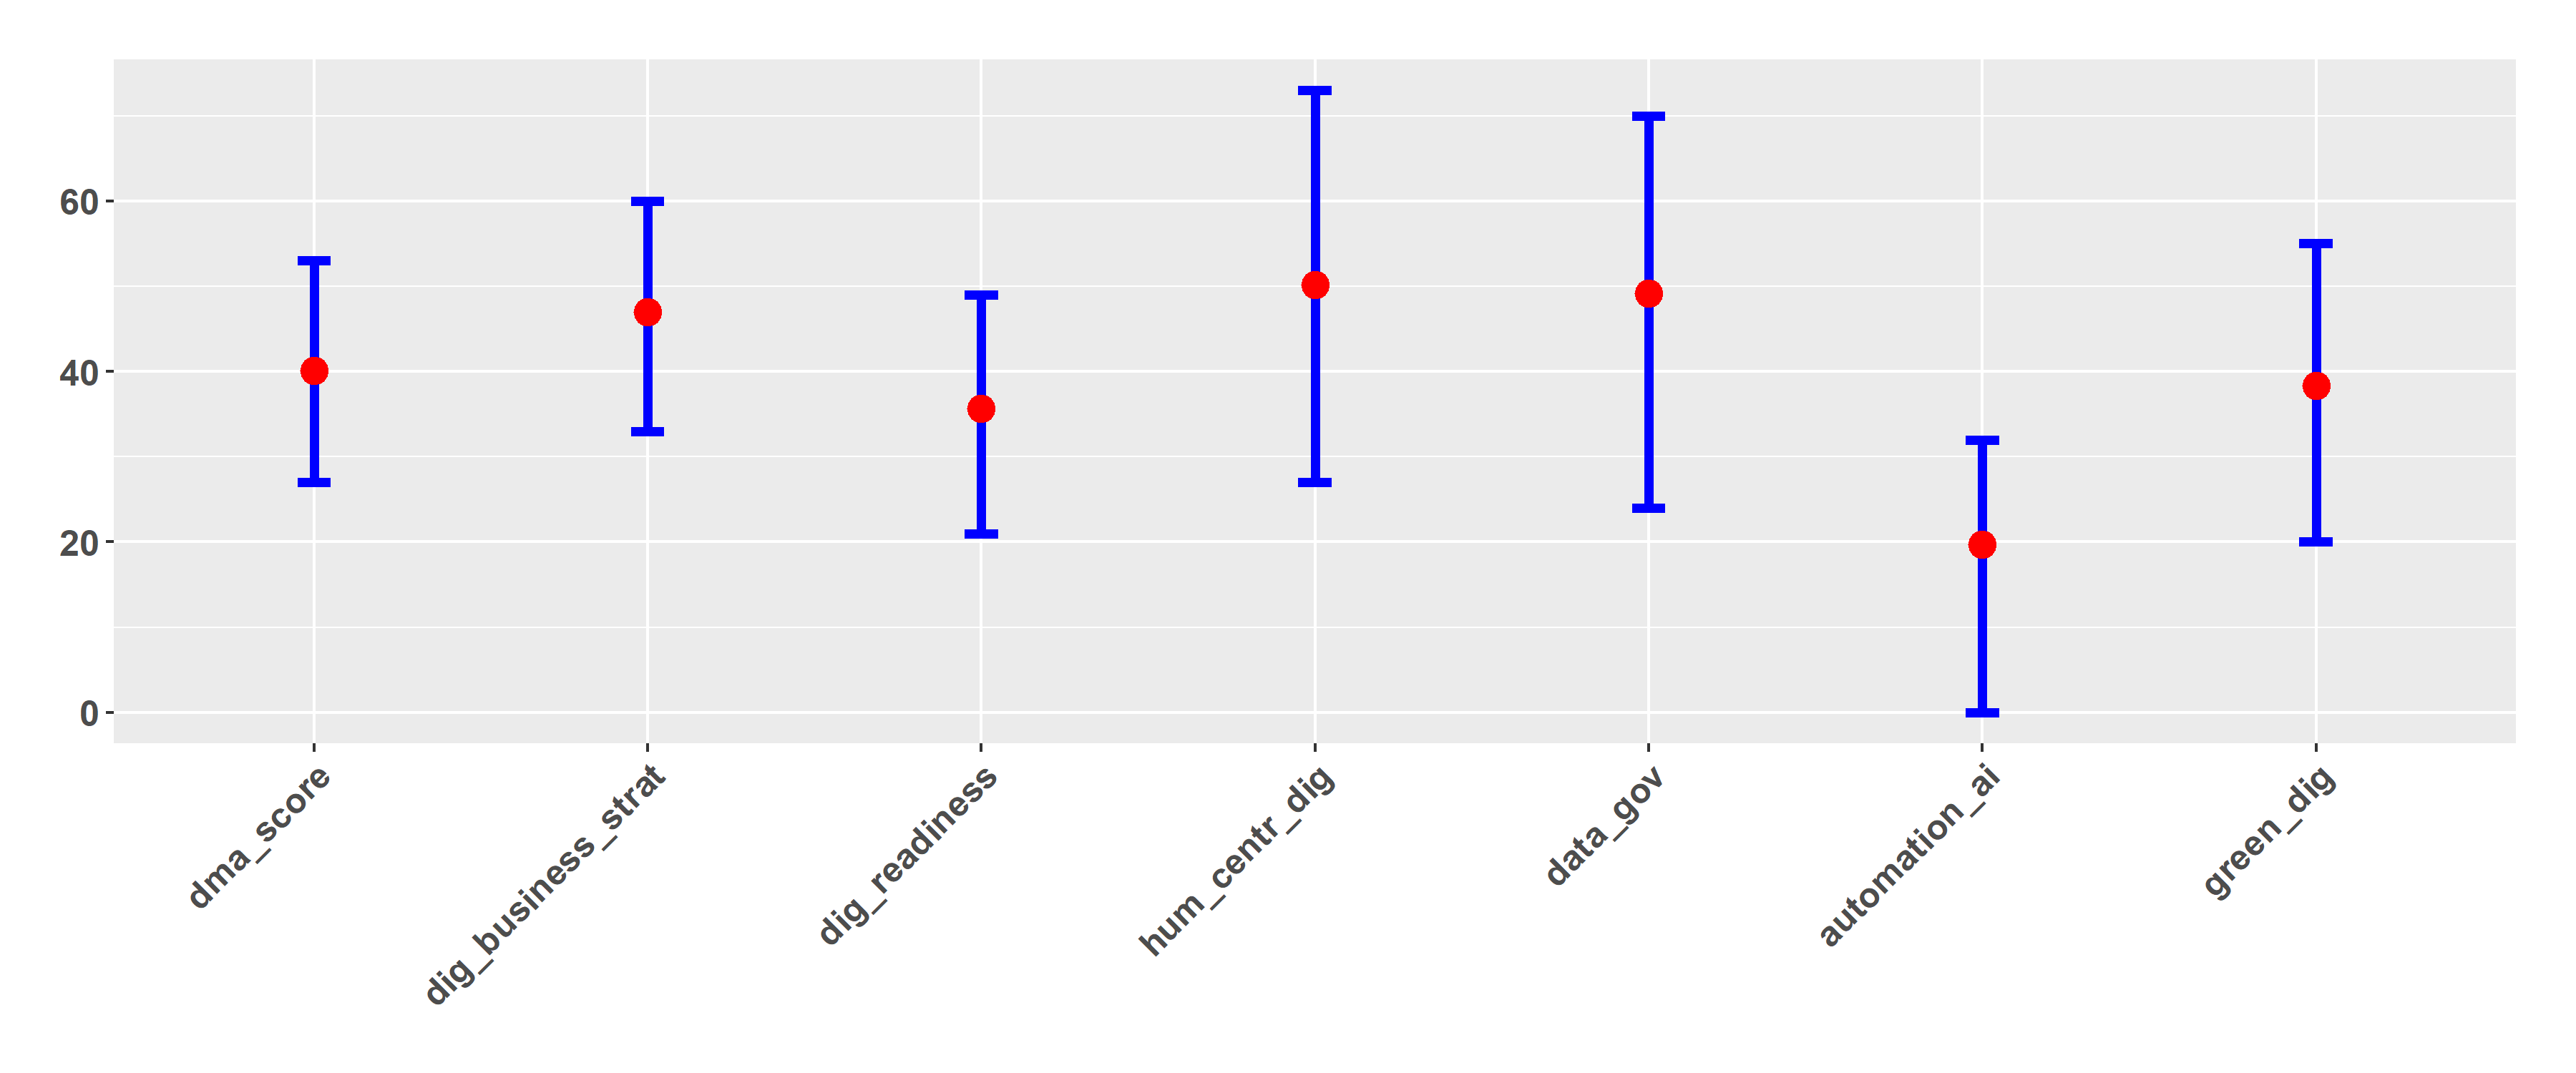
\includegraphics[width=\linewidth]{../Output/dma_score_quantiles.png}
    \caption{\centering{Average DMA dimension score and their 25-75 quantile intervals.}}
    \label{fig:dmascores_bydimension}
\end{figure}



\par We can now move over to an analysis of how scores are distributed across countries, sector, and size of the firm. Let's start with the country distribution. In the next figures you can see how the average DMA score and the average dimension score varies from country to country.

\begin{figure}[h!]
    \begin{center}
        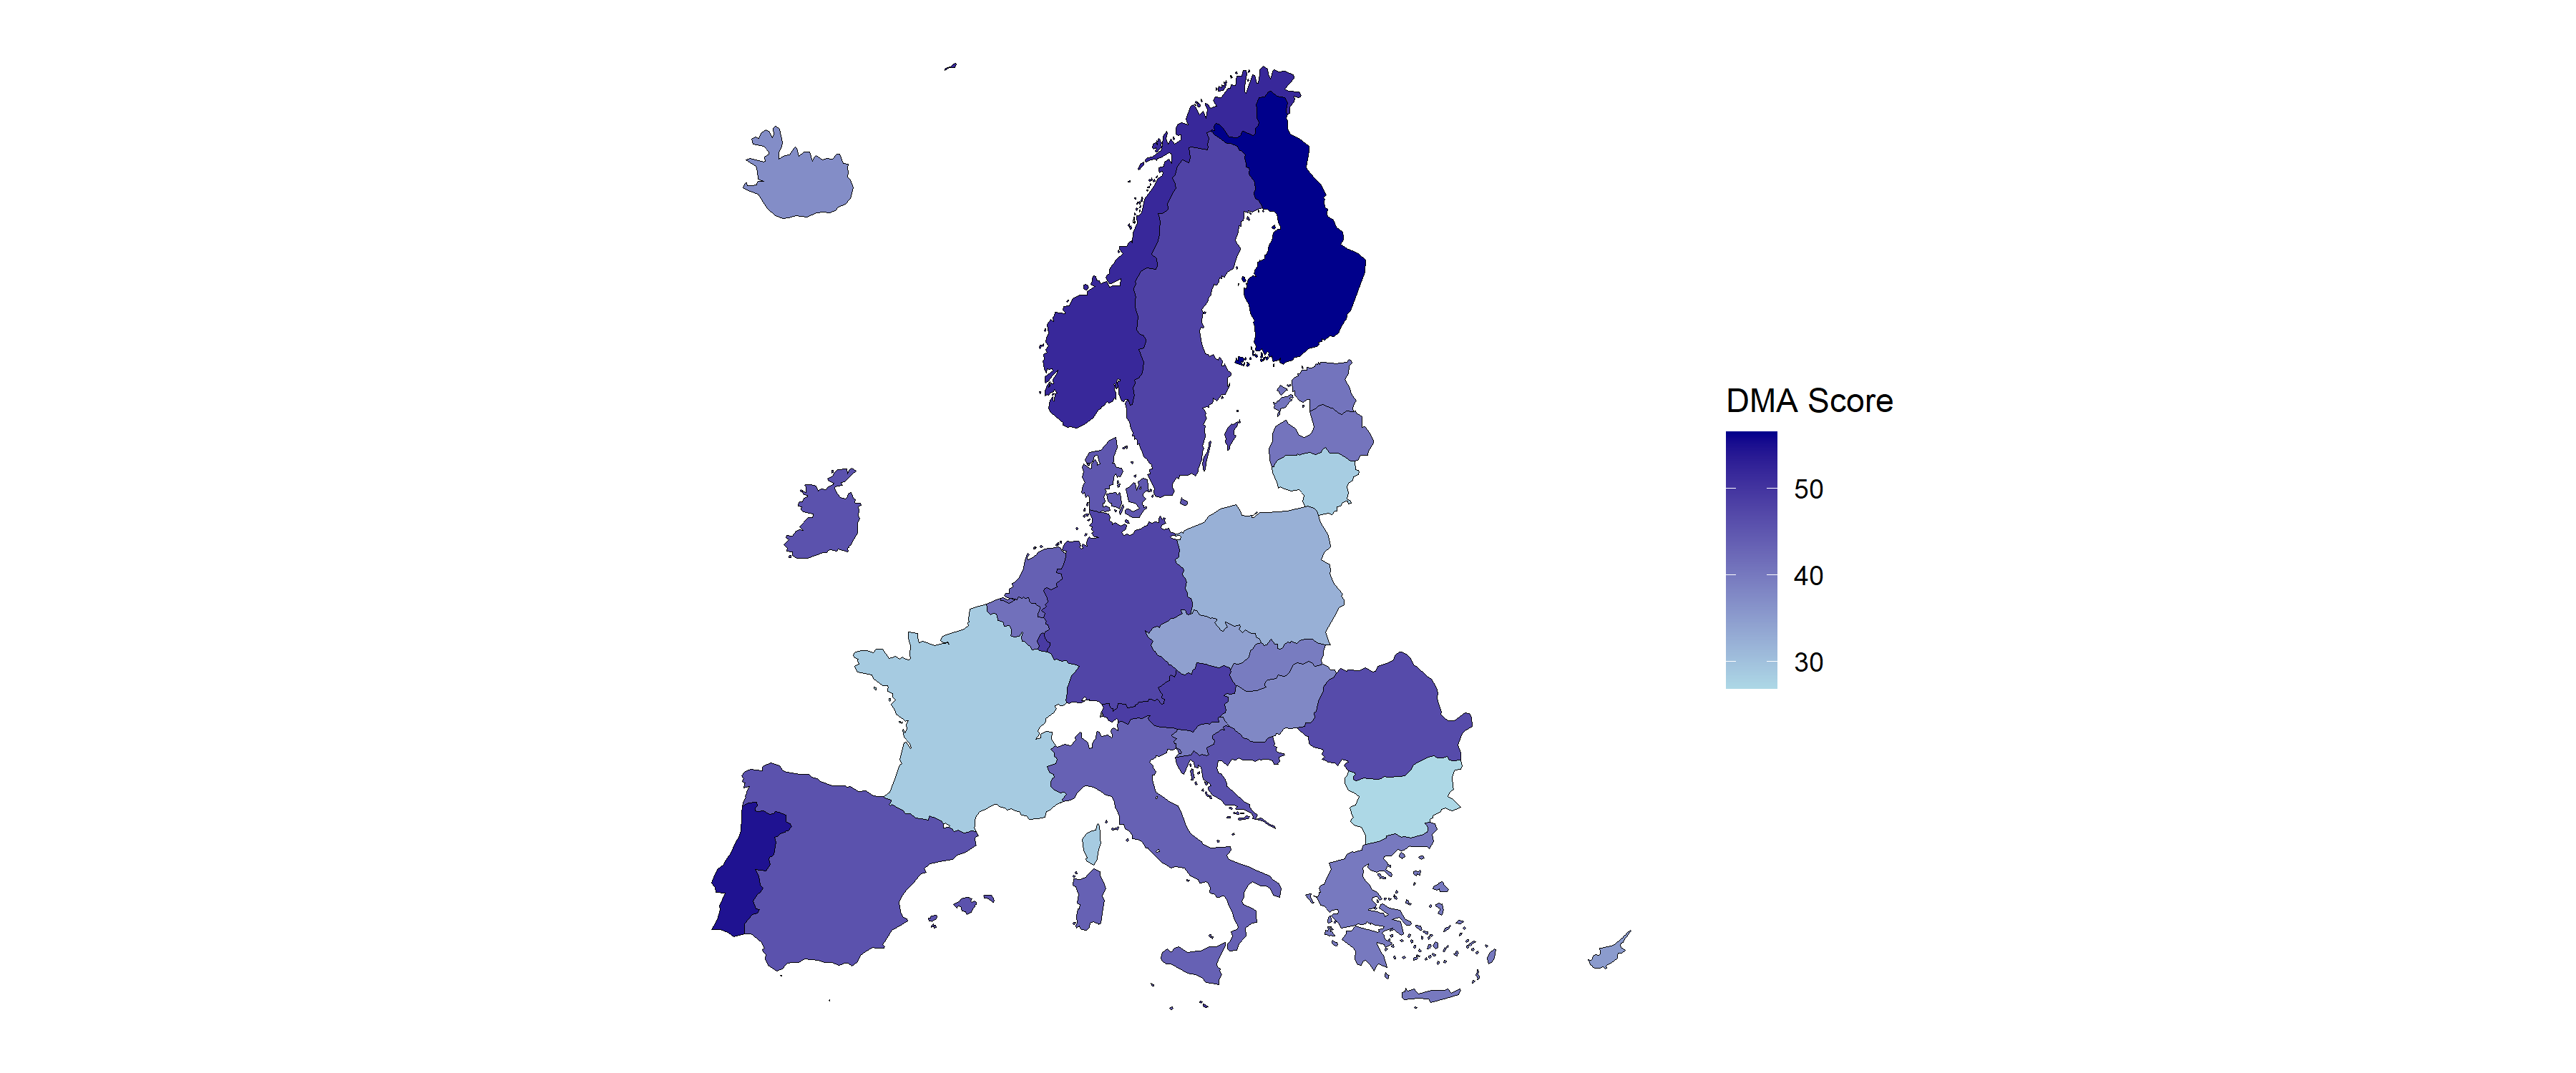
\includegraphics[width=0.6\textheight,trim=225 0 225 0,clip]{../Output/map5.png}        
        \caption{DMA score distribution by country}
        \label{fig:dma_score_country_map}
    \end{center}
\end{figure}



\begin{figure}[h!]
    \centering
    \begin{subfigure}[b]{0.49\textwidth}
        \centering
        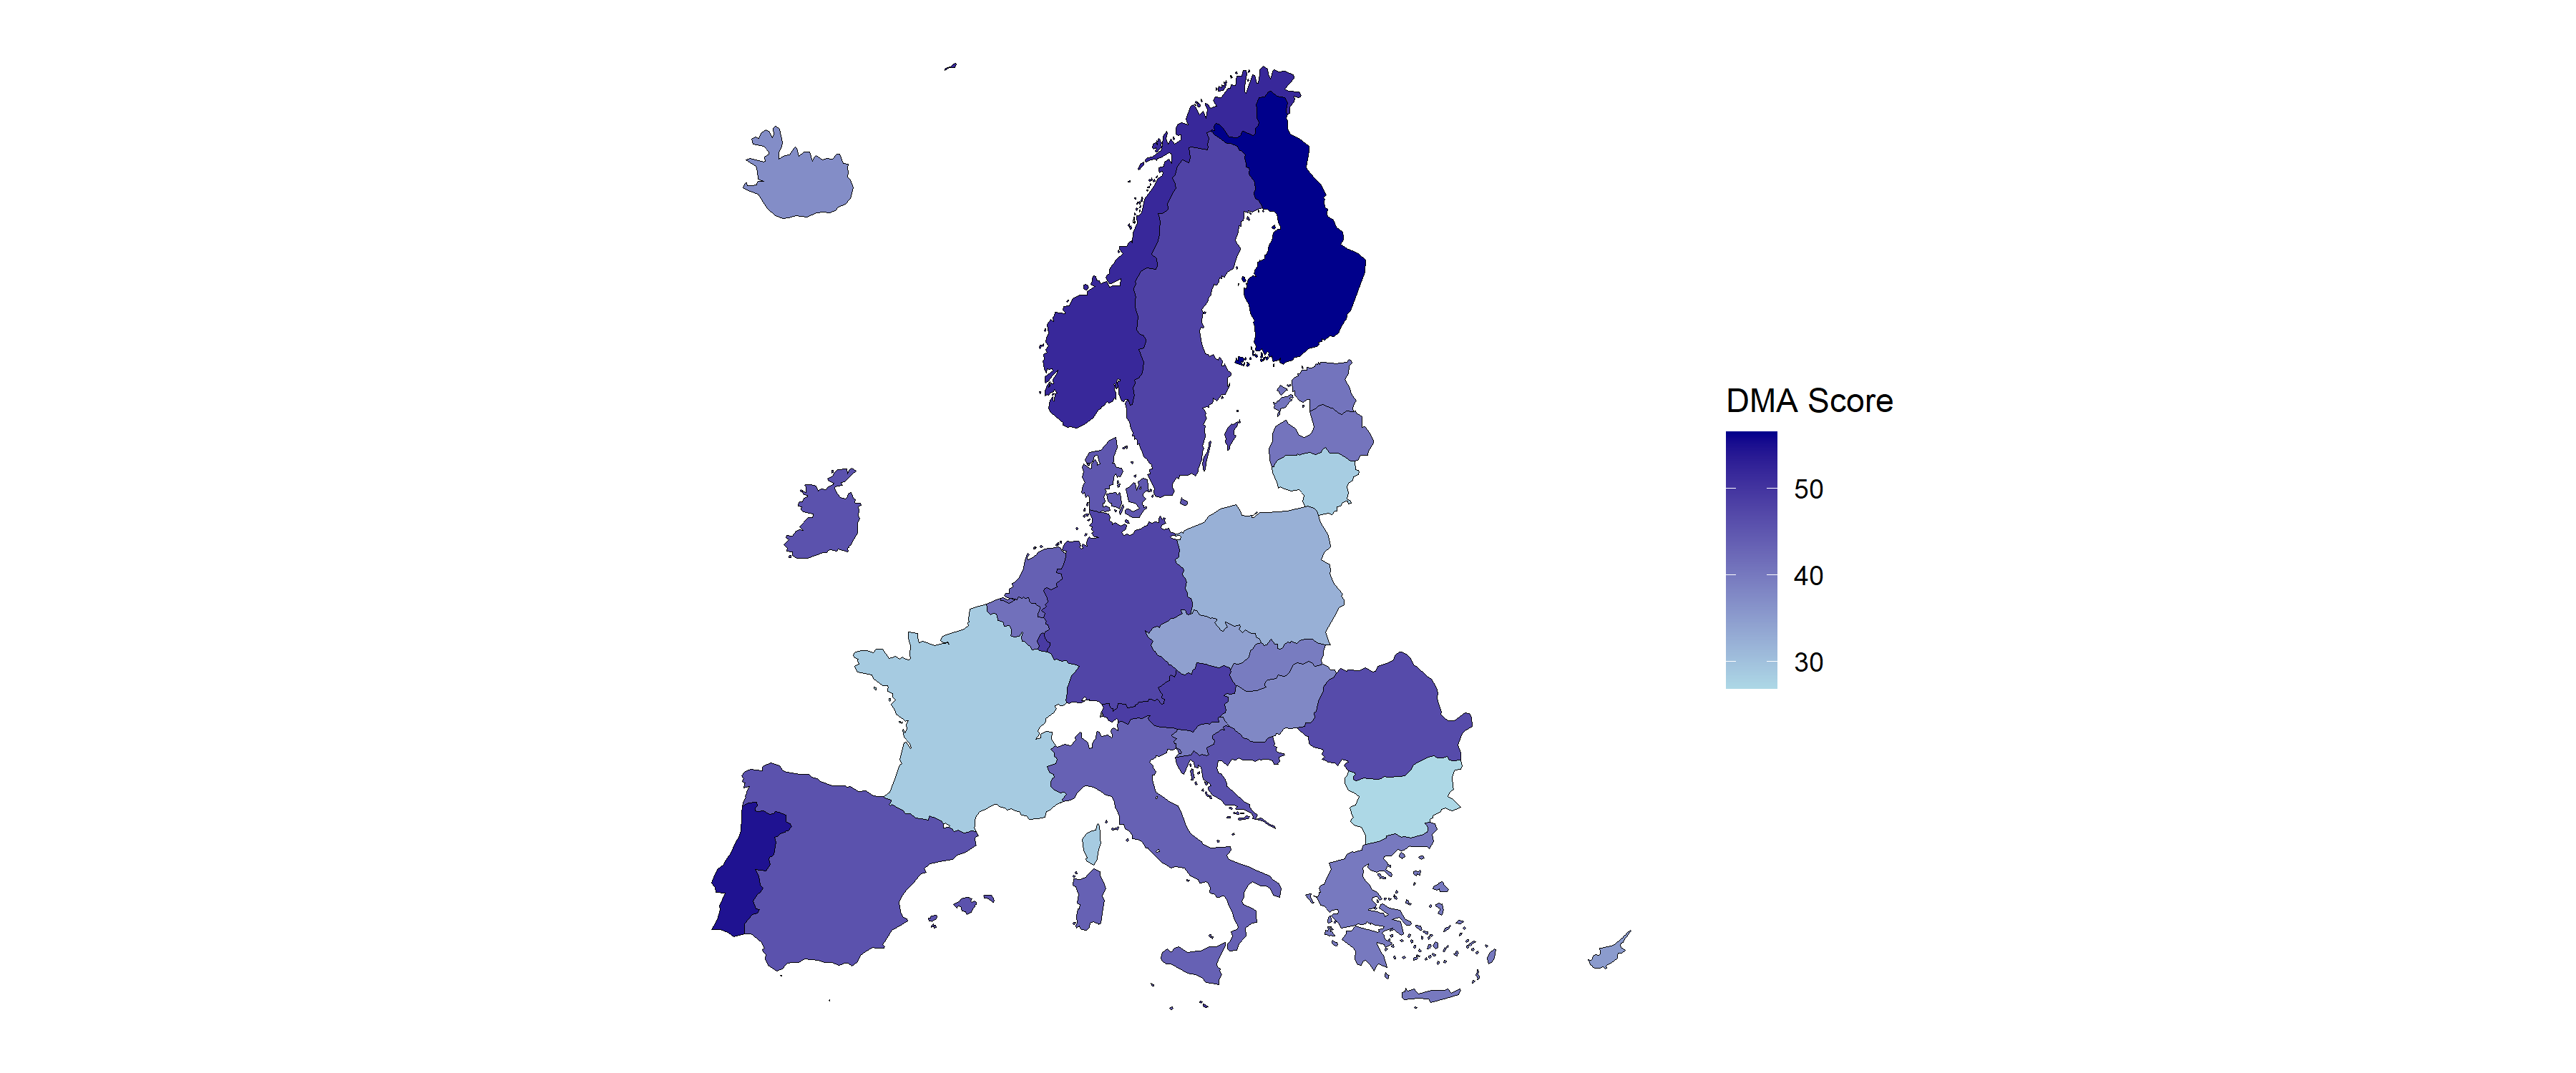
\includegraphics[width=0.3\textheight,trim=225 0 225 0,clip]{../Output/map5.png}        
        \caption{Digital Business Strategy}
        \label{fig:map12}
    \end{subfigure}
    \hfill
    \begin{subfigure}[b]{0.49\textwidth}
        \centering
        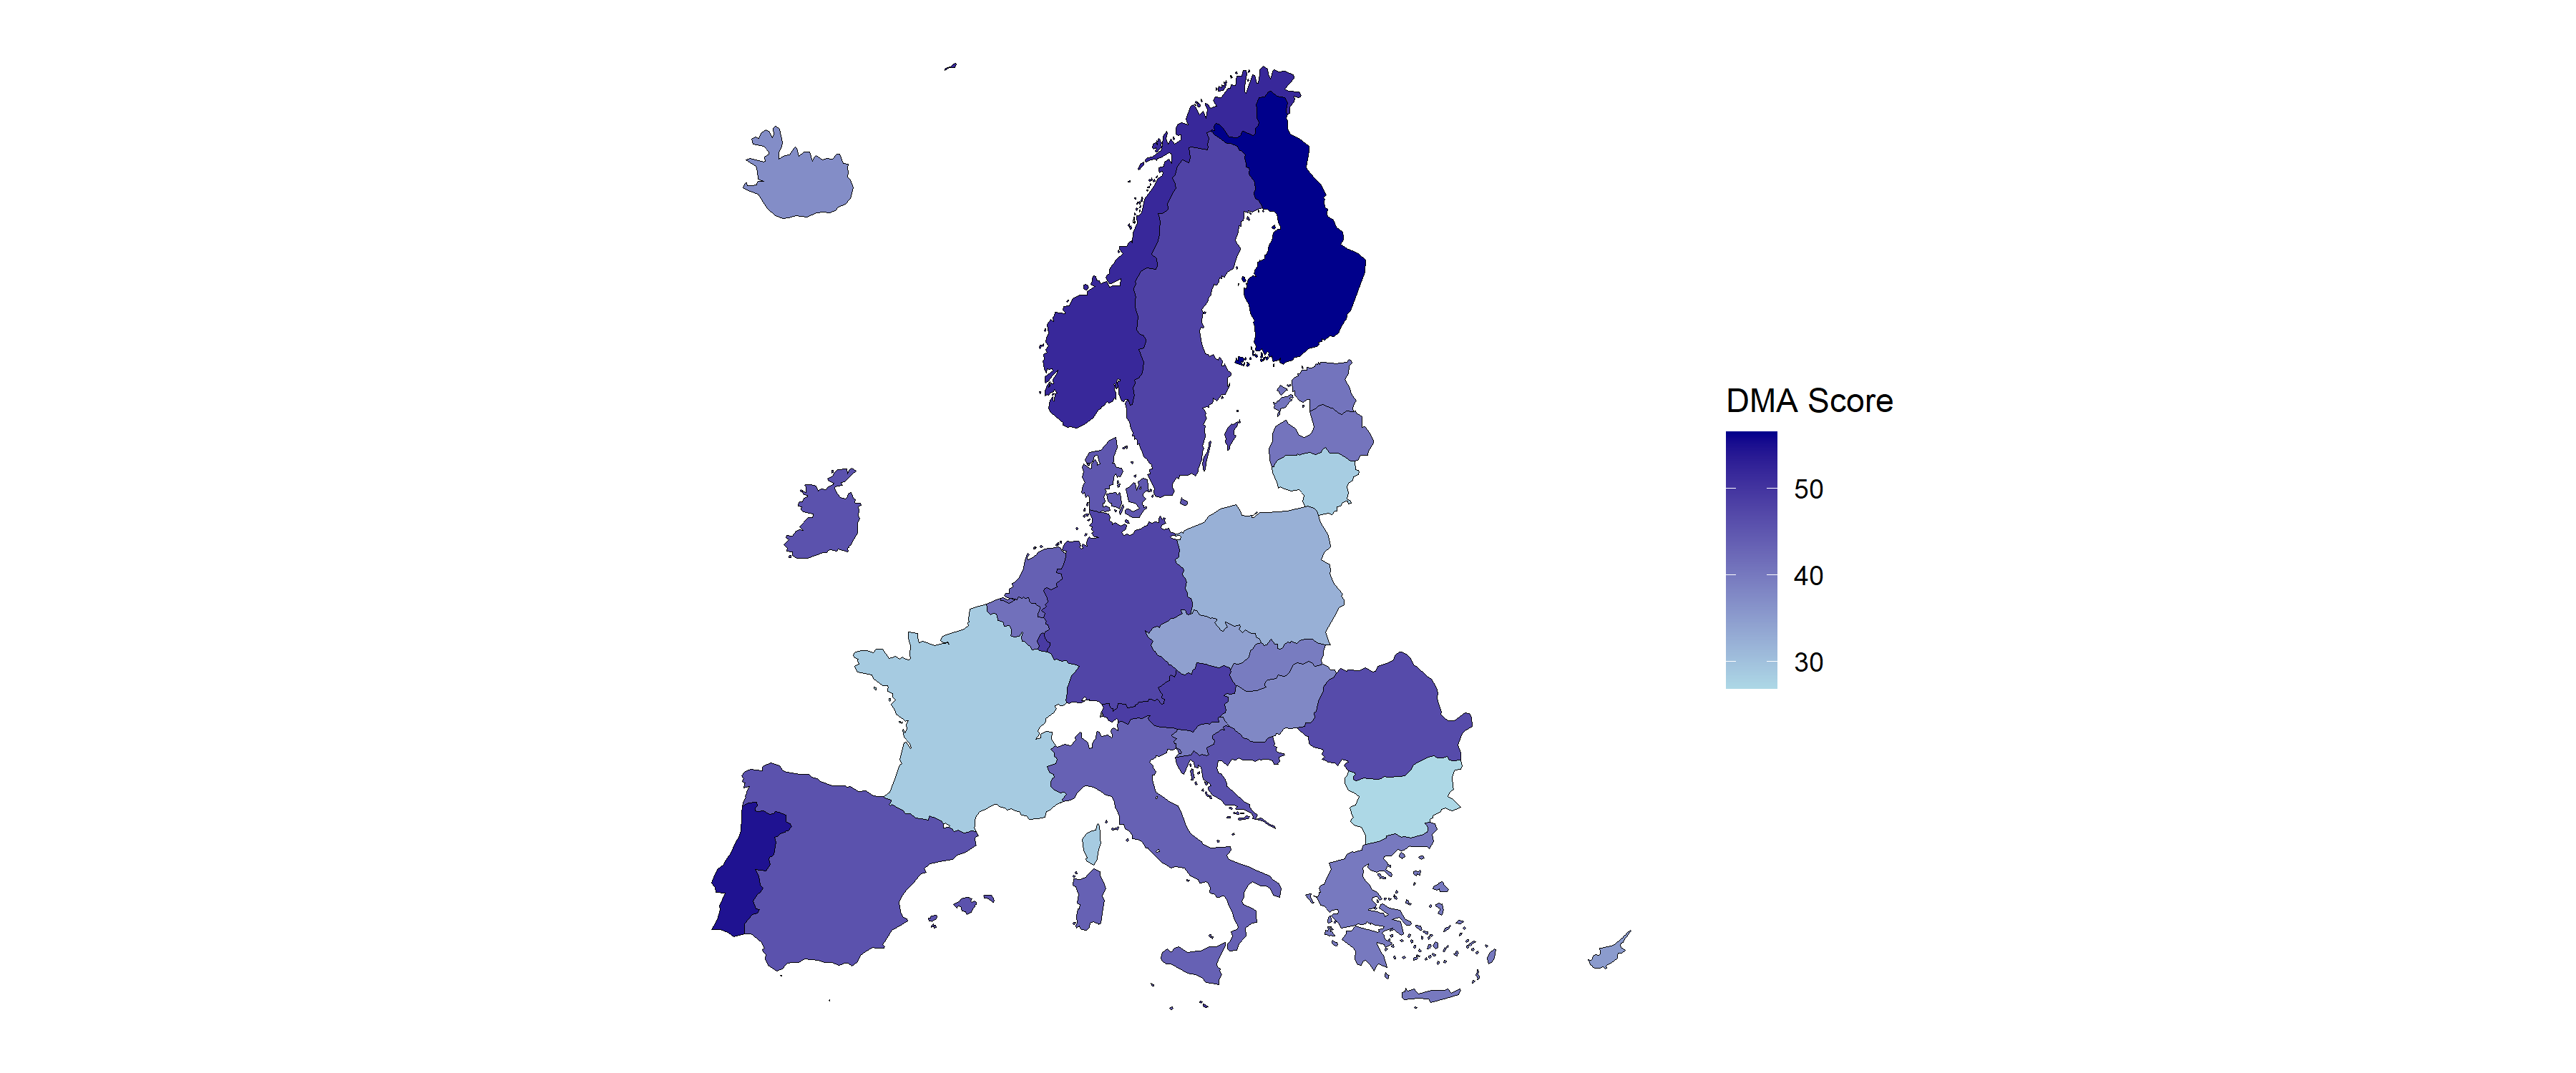
\includegraphics[width=0.3\textheight,trim=225 0 225 0,clip]{../Output/map5.png}        
        \caption{Digital Readiness}
        \label{fig:map13}
    \end{subfigure}
    \vfill
    \begin{subfigure}[b]{0.49\textwidth}
        \centering
        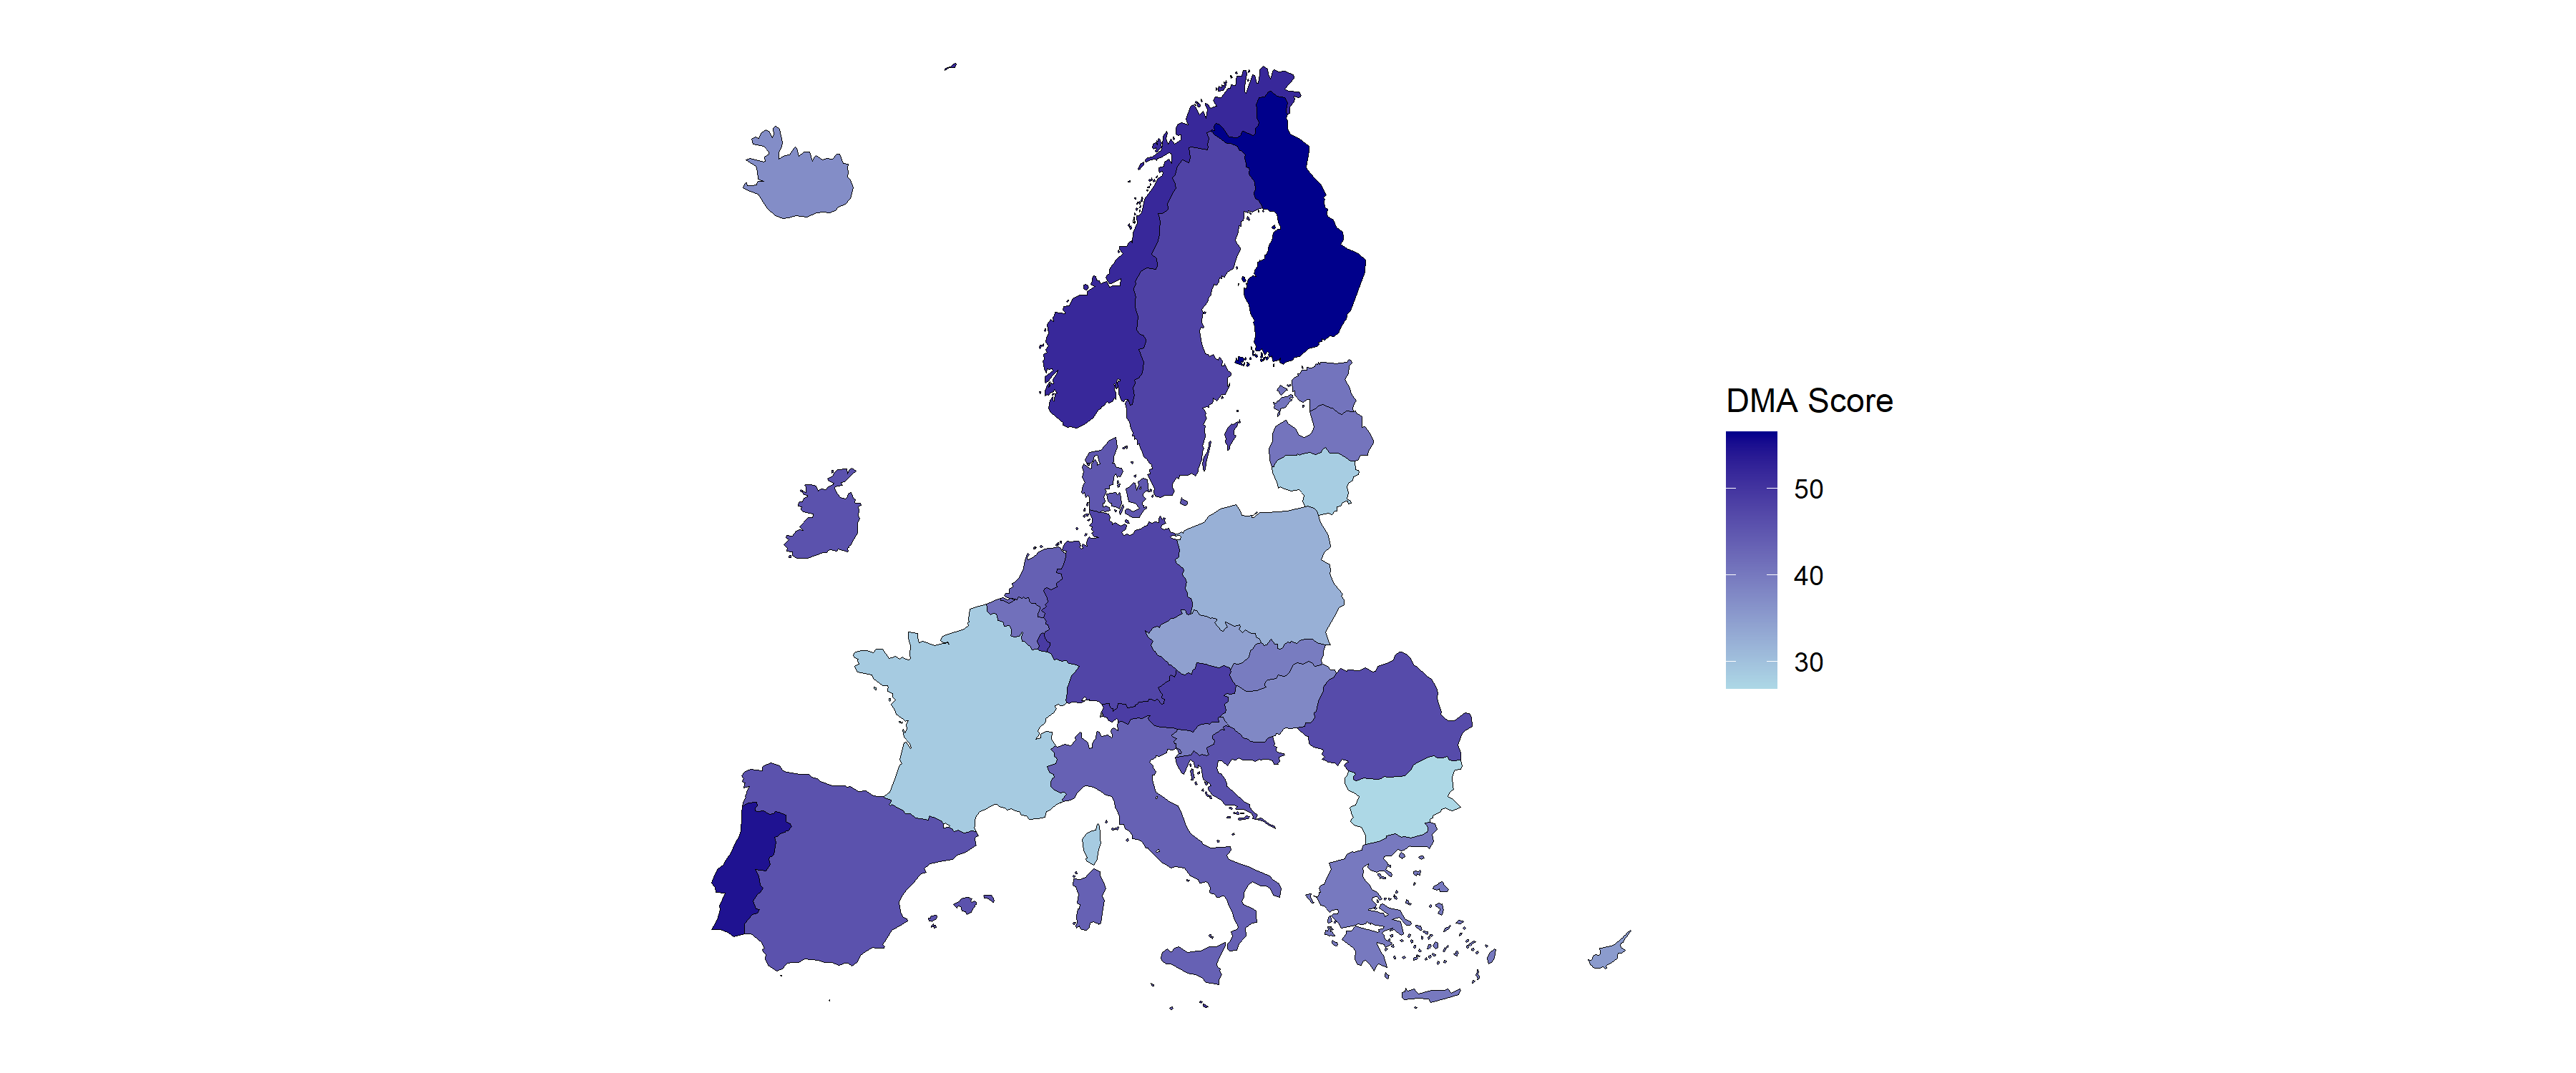
\includegraphics[width=0.3\textheight,trim=225 0 225 0,clip]{../Output/map5.png}        
        \caption{Human-Centric Digitalization}
        \label{fig:map14}
    \end{subfigure}
    \hfill
    \begin{subfigure}[b]{0.49\textwidth}
        \centering
        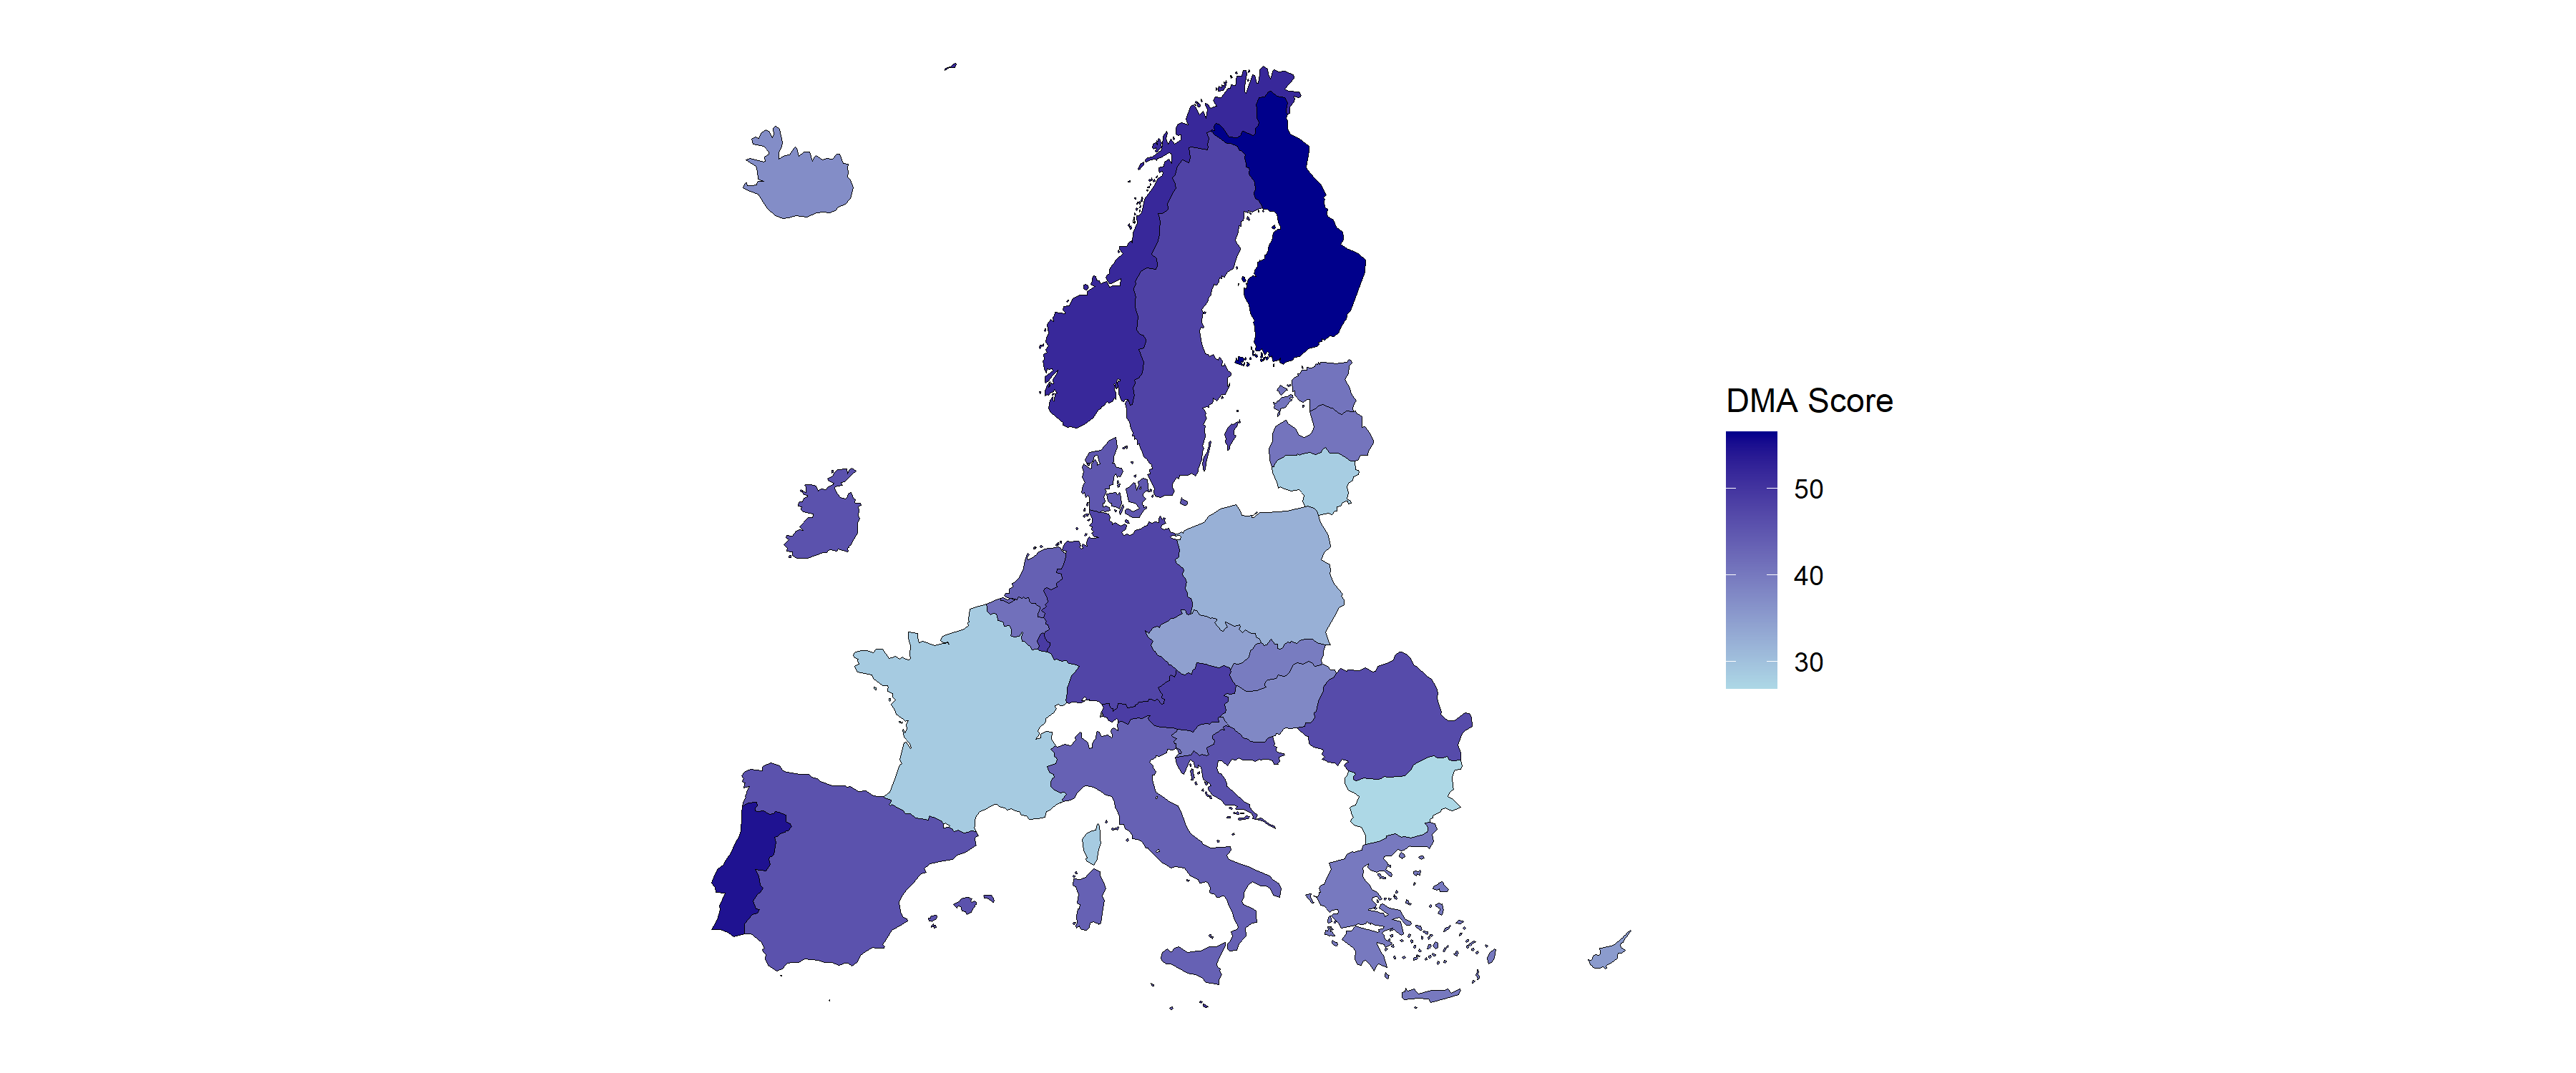
\includegraphics[width=0.3\textheight,trim=225 0 225 0,clip]{../Output/map5.png}        
        \caption{Data Management}
        \label{fig:map15}
    \end{subfigure}
    \vfill
    \begin{subfigure}[b]{0.49\textwidth}
        \centering
        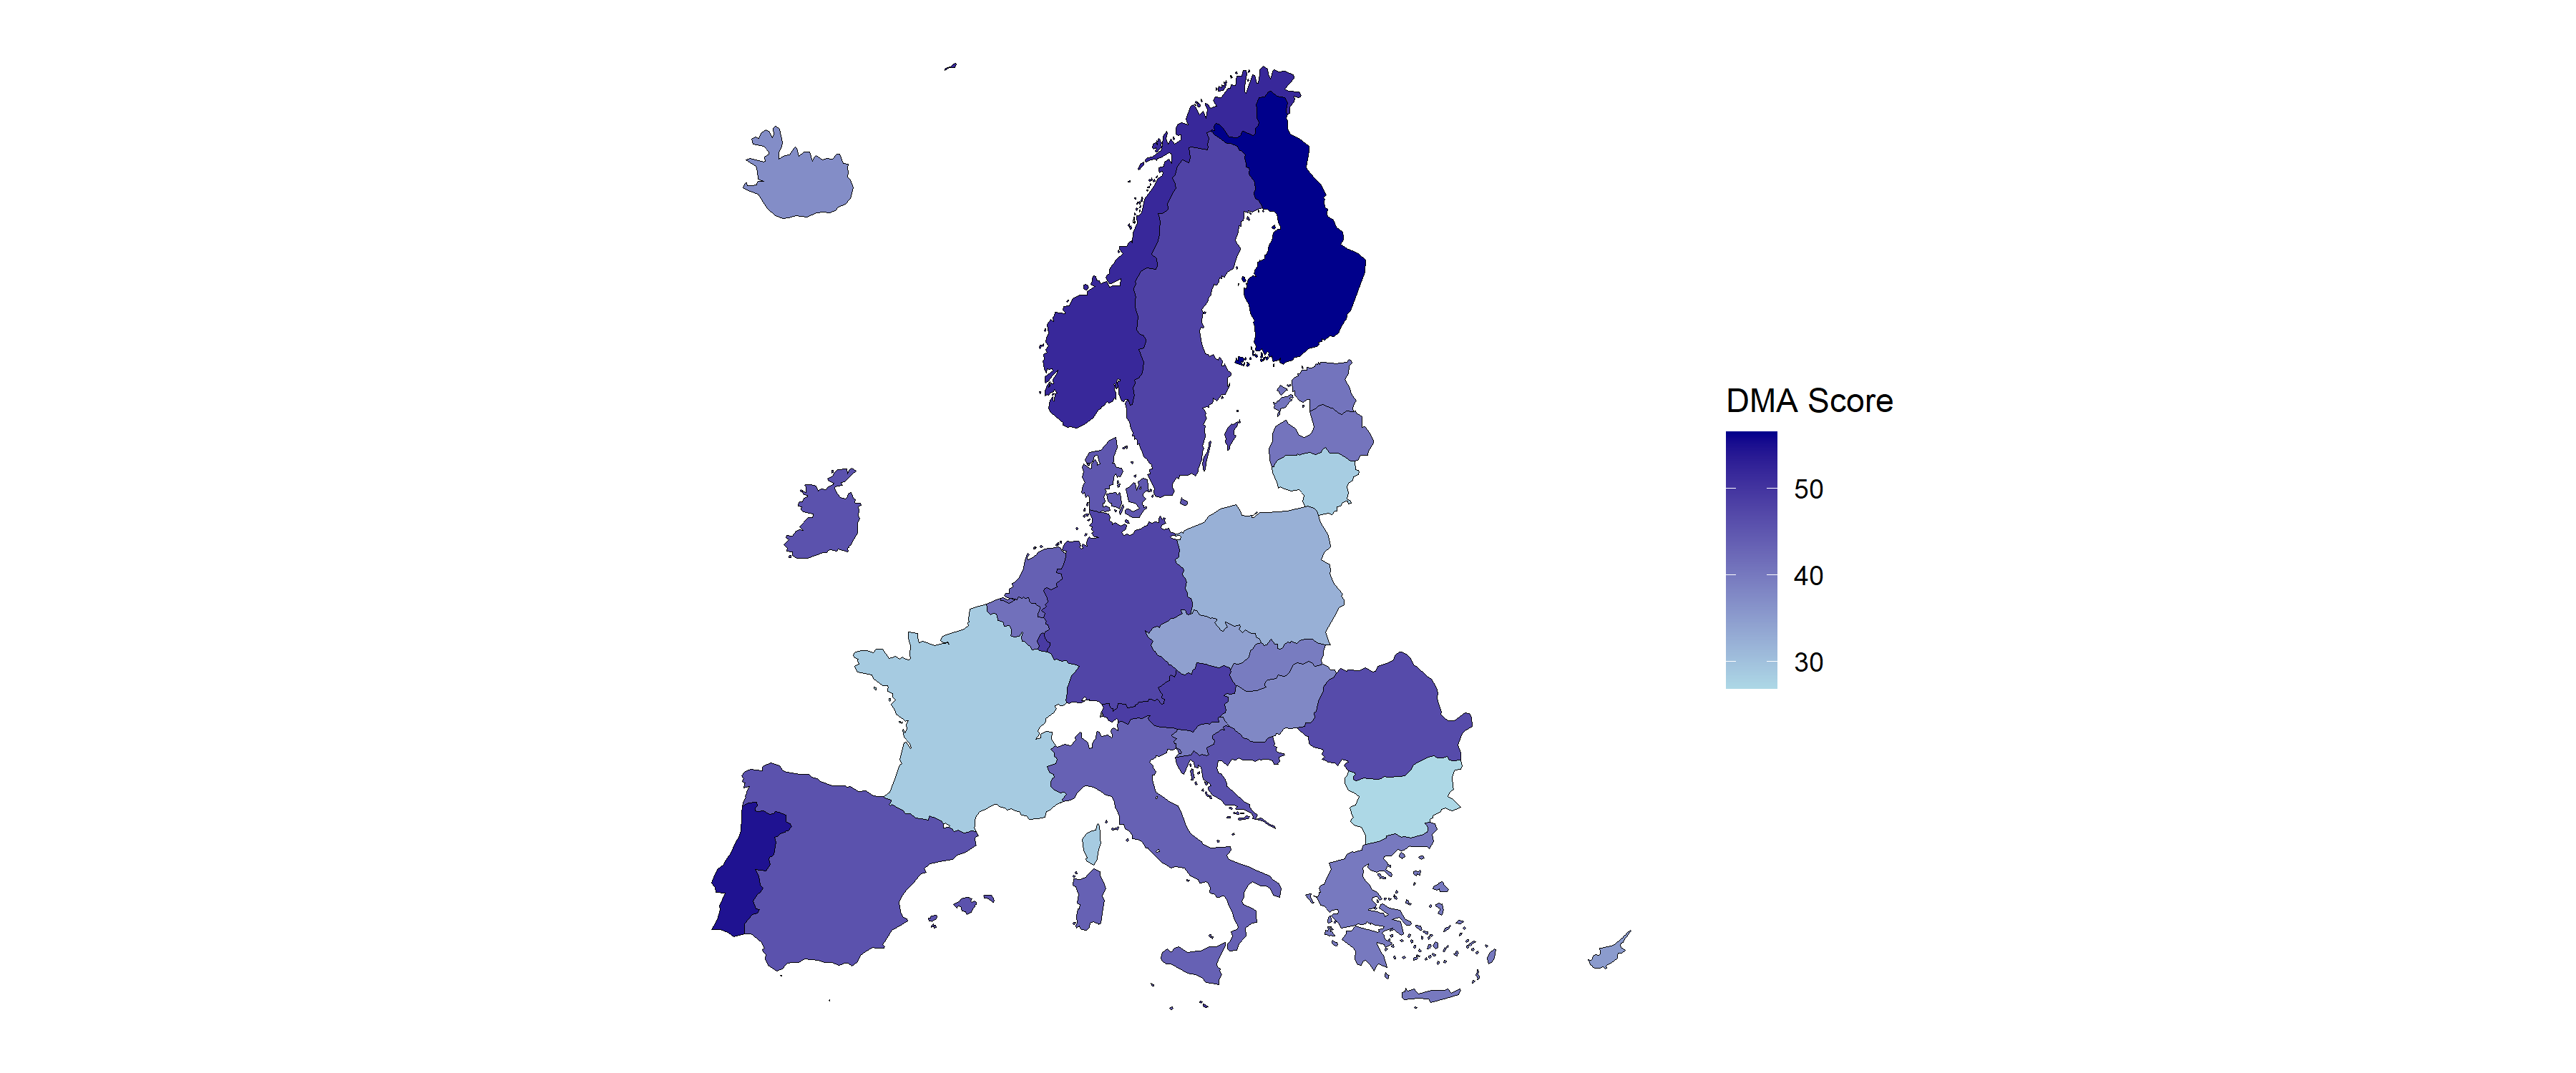
\includegraphics[width=0.3\textheight,trim=225 0 225 0,clip]{../Output/map5.png}        
        \caption{Automation \& Intelligence}
        \label{fig:map16}
    \end{subfigure}
    \hfill
    \begin{subfigure}[b]{0.49\textwidth}
        \centering
        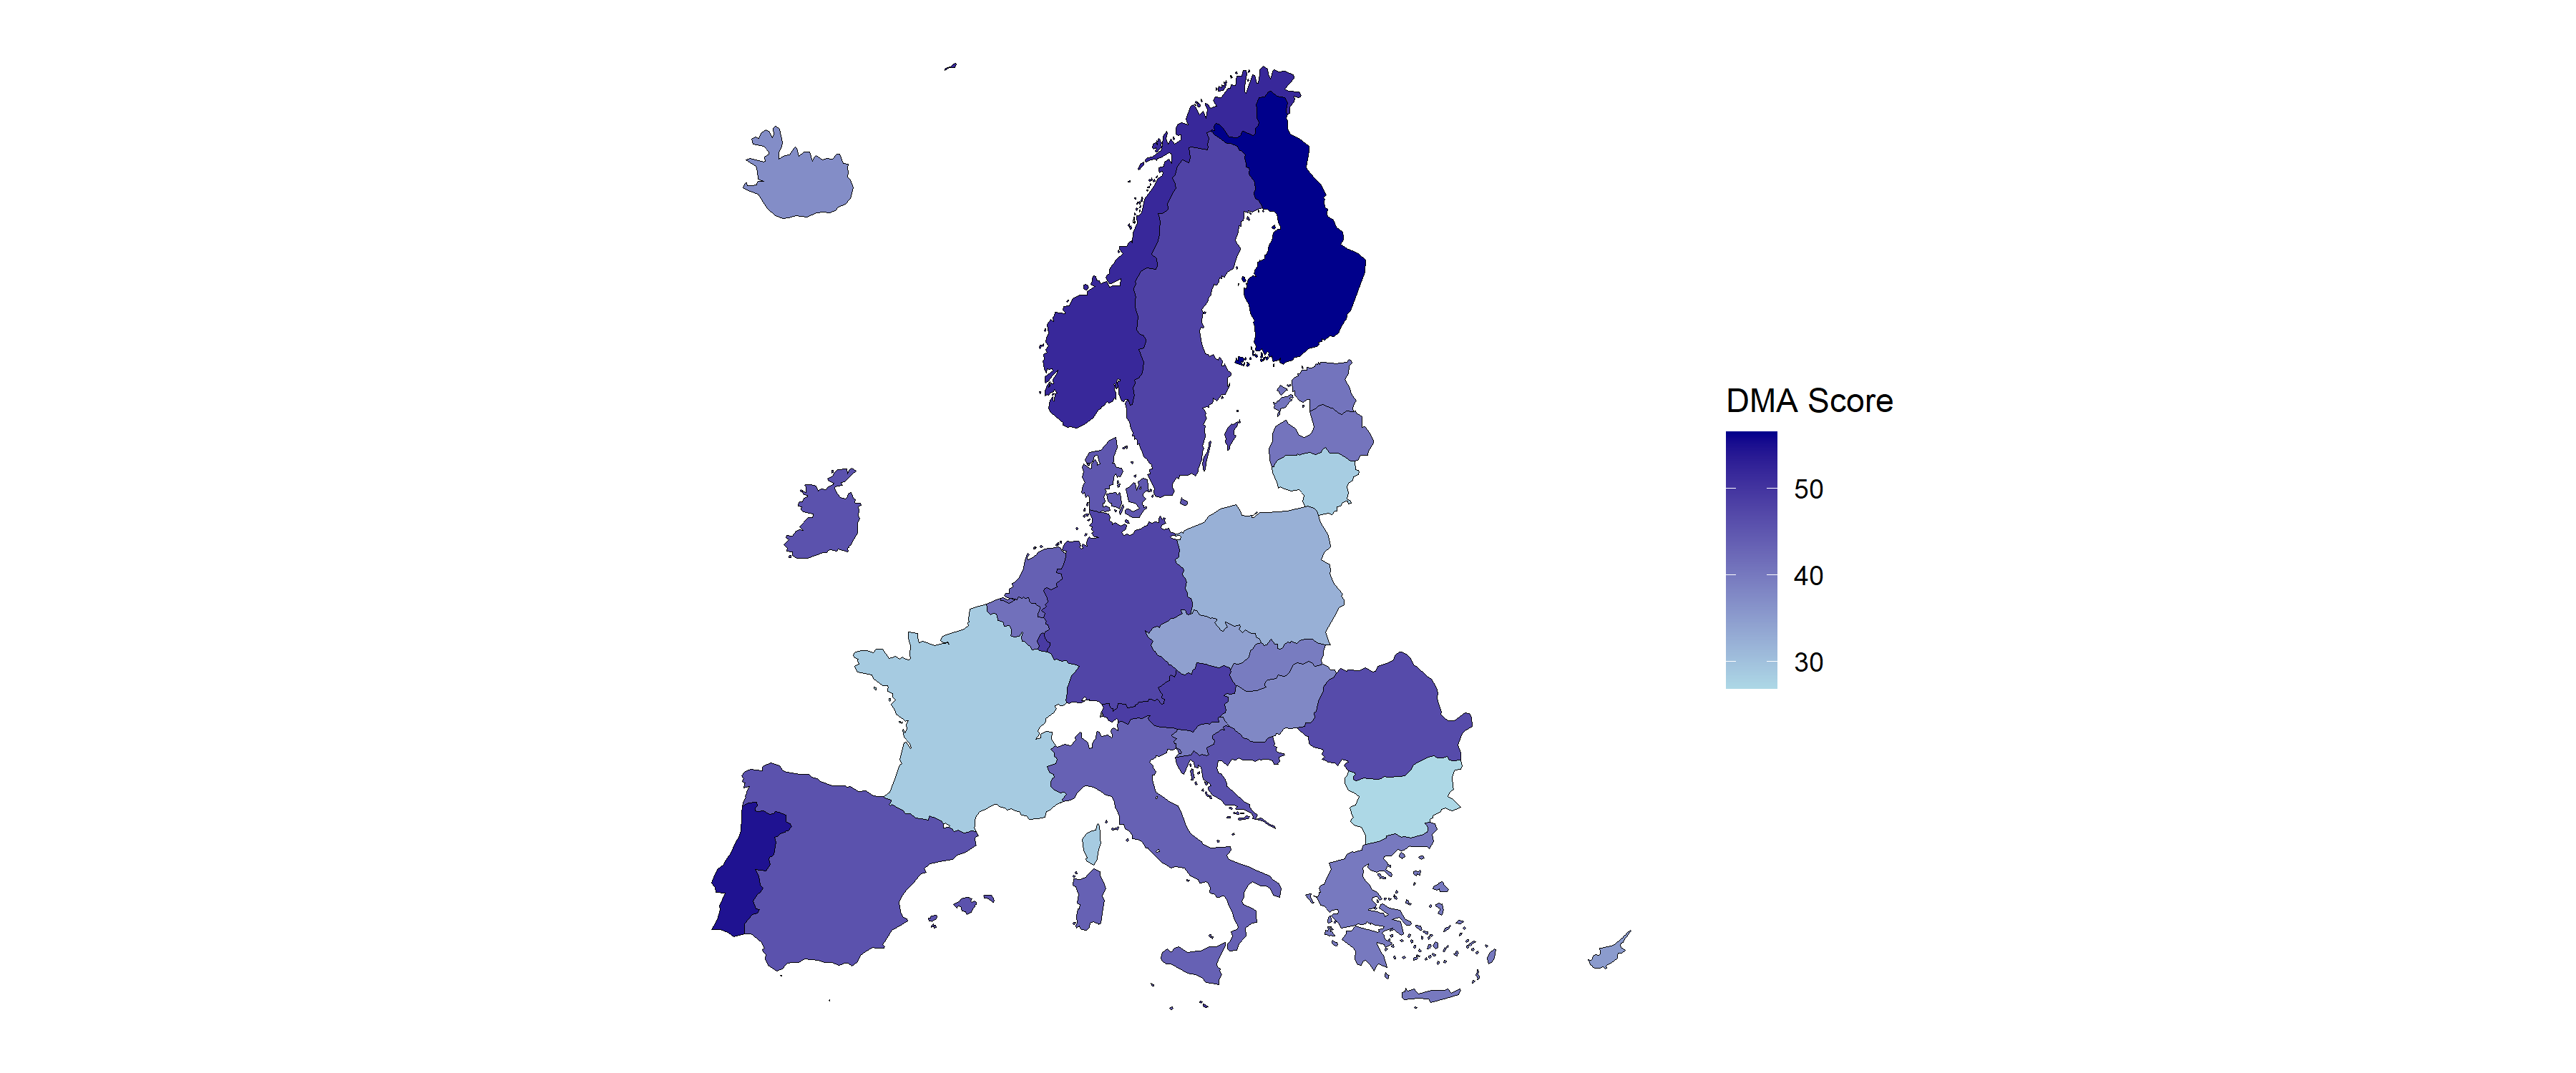
\includegraphics[width=0.3\textheight,trim=225 0 225 0,clip]{../Output/map5.png}        
        \caption{Green Digitalization}
        \label{fig:map17}
    \end{subfigure}
    \caption{Distribution of all dimensions' scores by country}
    \label{fig:dma_maps}
\end{figure}

\par Right away with the overall DMA score's geographical distribution we can notice how the score is significantly higher in the nordic countries. However, very good scores come also from southern countries such as Italy or Spain (Portugal is also very high, but the sample size is very low). Curiously, one of the worst-performing countries is France. We can see from the breakdown of components how this is not due to a specific dimension, as France performs badly in all of them, suggesting a lower level of digital maturity of the sampled firms in France.

\par In the Automation \& Intelligence dimension, which is the one with lowest average score overall, we can see how the only countries having a slight edge are Austria and Finland, probably signalling a higher proportion of technologically intensive firms in these countries' sample.

\par If we analyze the distribution of scores by sector instead, we see how more technologically-intensive sectors have on average higher levels of Digital Maturity. In fact, the highest average DMA belongs to the Telecommunications sector, followed by the Environment sector, Transport \& Mobility and Metal Working. Interestingly, a sector that we would expect to be exposed to digitalization presents instead a low DMA score: that is the case of the Financial services sector. Overall though, we see how the average DMA score is lower for those sectors that have had limited exposure to digitalization, as our prior knowledge would suggest.

\begin{figure}[h!]
    \centering
    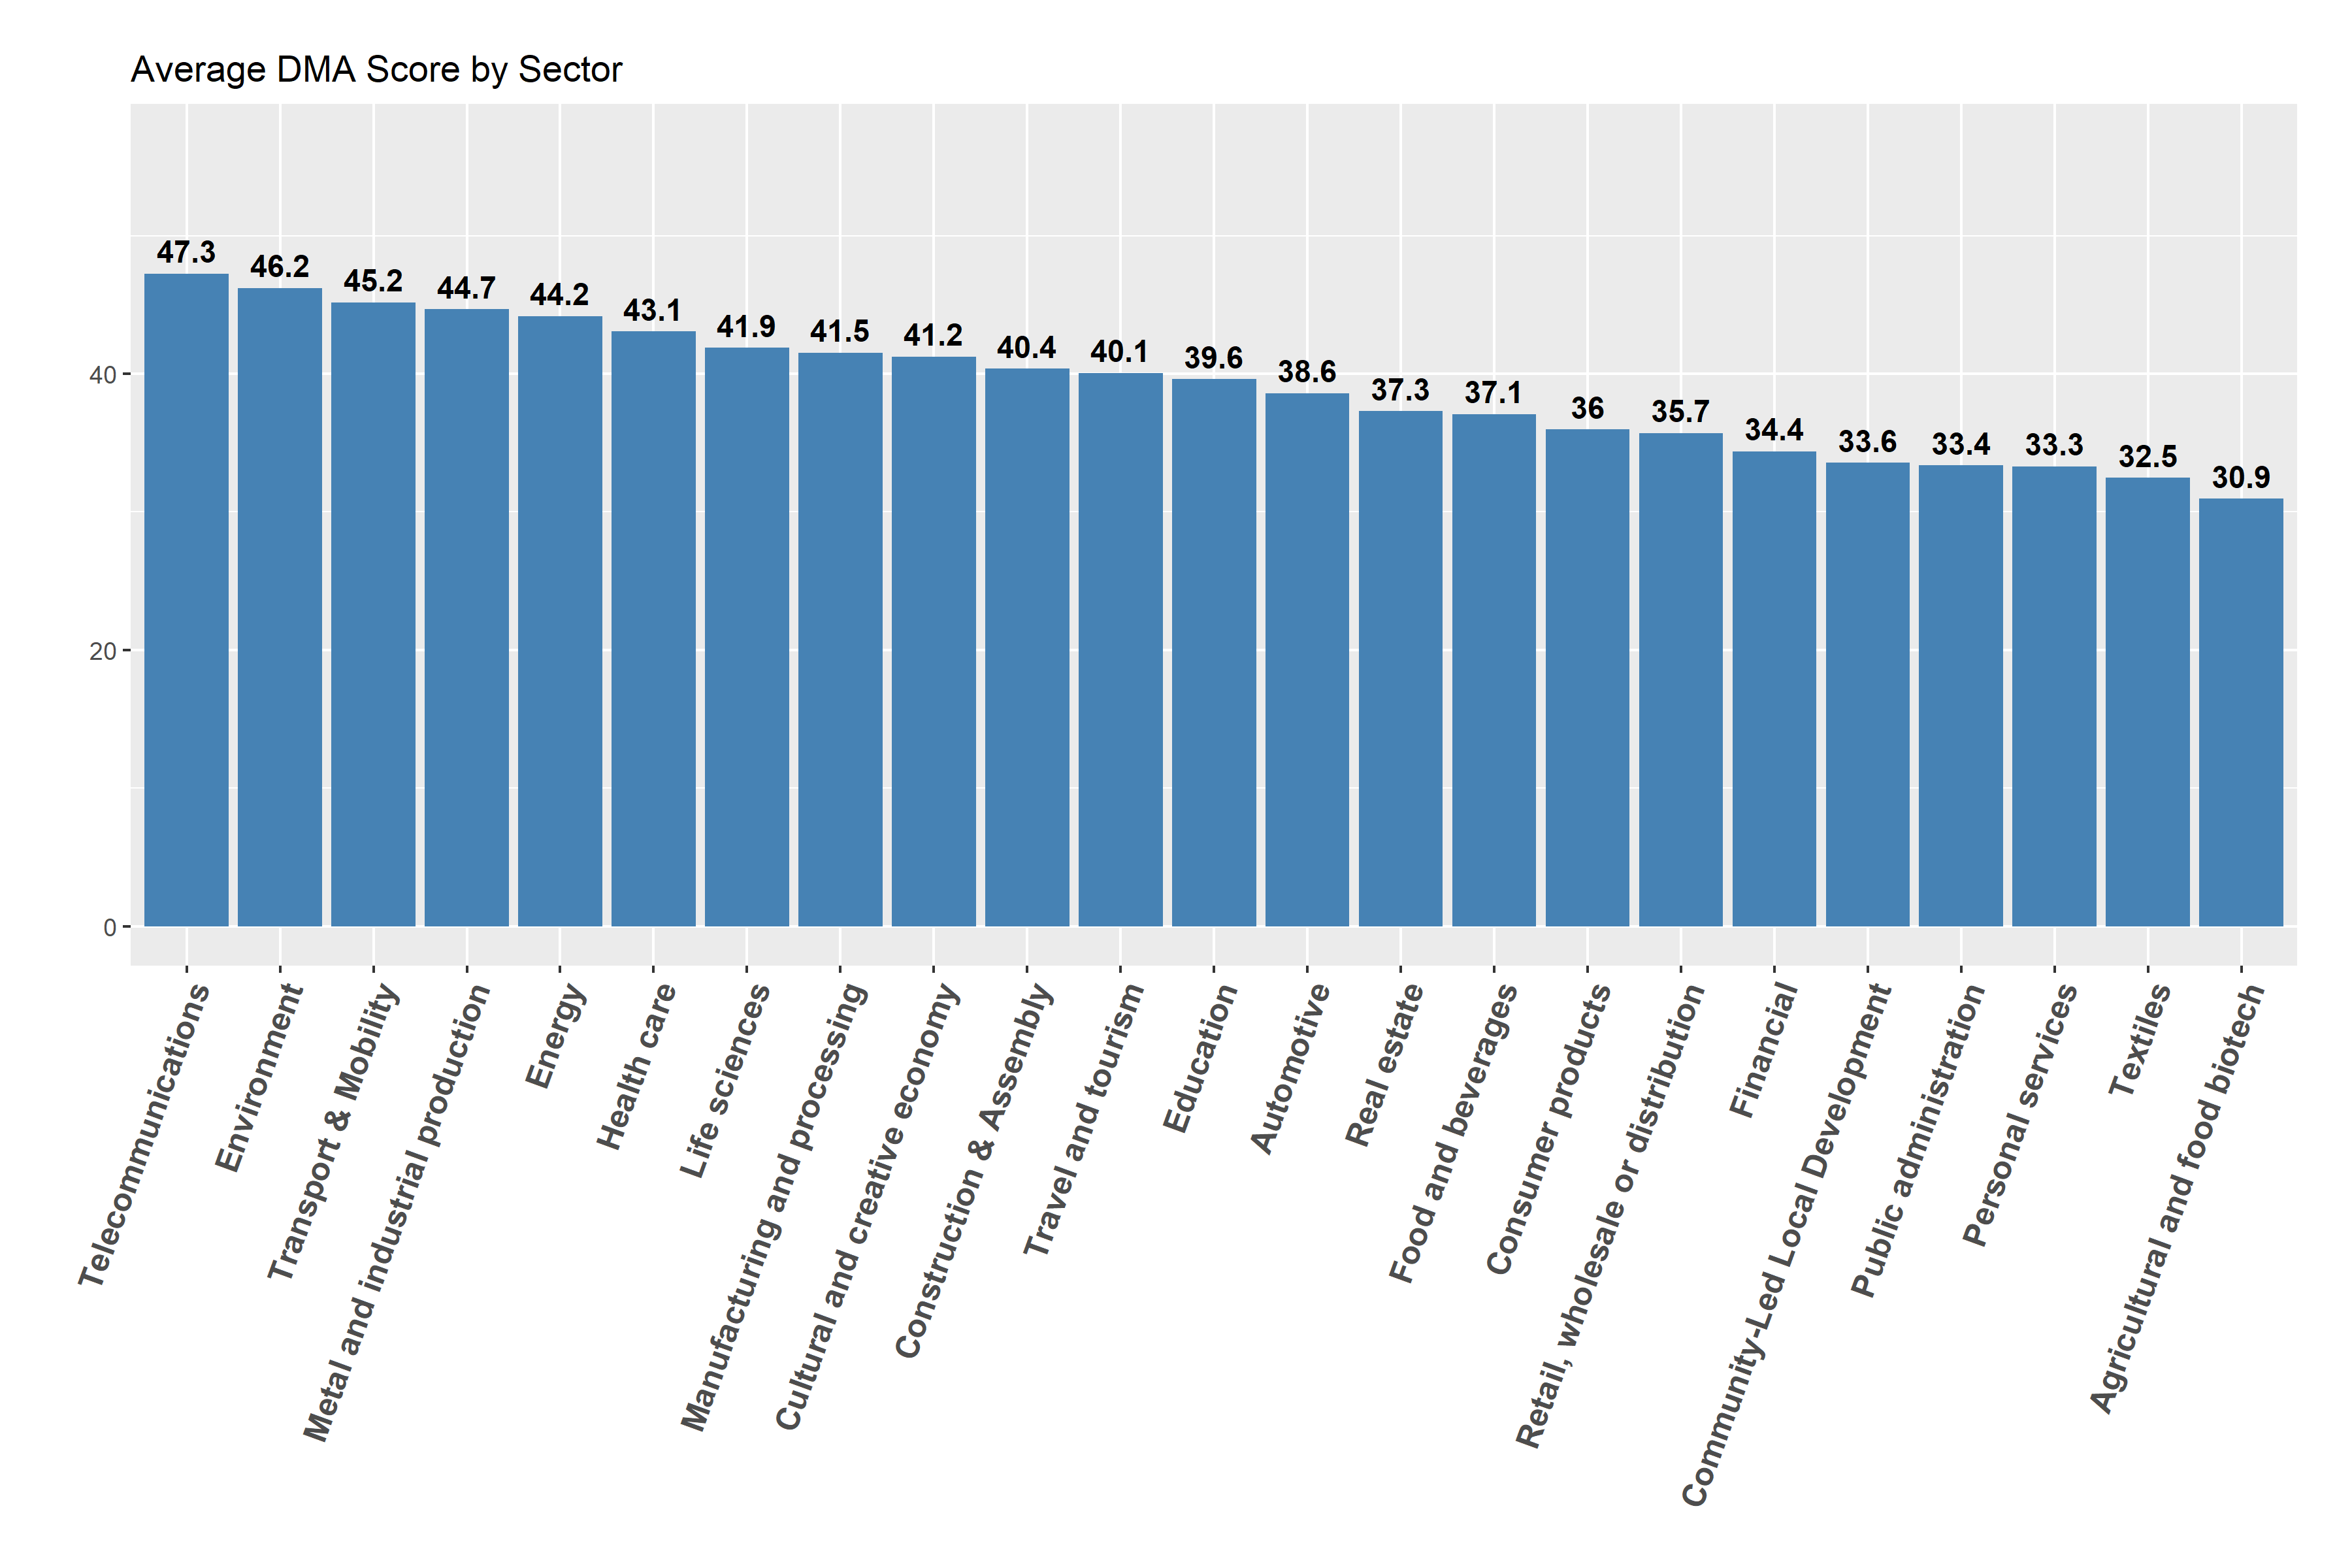
\includegraphics[width=\linewidth]{../Output/avg_dmascore_by_sector.png}
    \caption{\centering{Distribution of the average DMA score across sectors of activity, as reported in the DMA, Module 1. Note that only sectors with more than 30 observations are considered.}}
    \label{fig:dma_sector_chart}
\end{figure}




\par Looking at the distribution of scores by size instead, we would expect to see a positive relationship between size and the average DMA score. In fact, this is exactly what we observe in our sample. This confirms the prior belief at the base of the EDIH initiative itself, being that the initiative should be focused on the digitalization of SMEs, since smaller firms are the ones struggling the most with the process. The lower levels of digital maturity observed in smaller firms can also explain at least part of the current gap in digitalization the EU is experiencing. Since firm size in most European member state is smaller on average than in other advanced economies (for example compared to the US), it is possible that part of the EU lag in adoption of digital technologies is due to insufficient firm size.
 

\begin{figure}[h!]
    \centering
    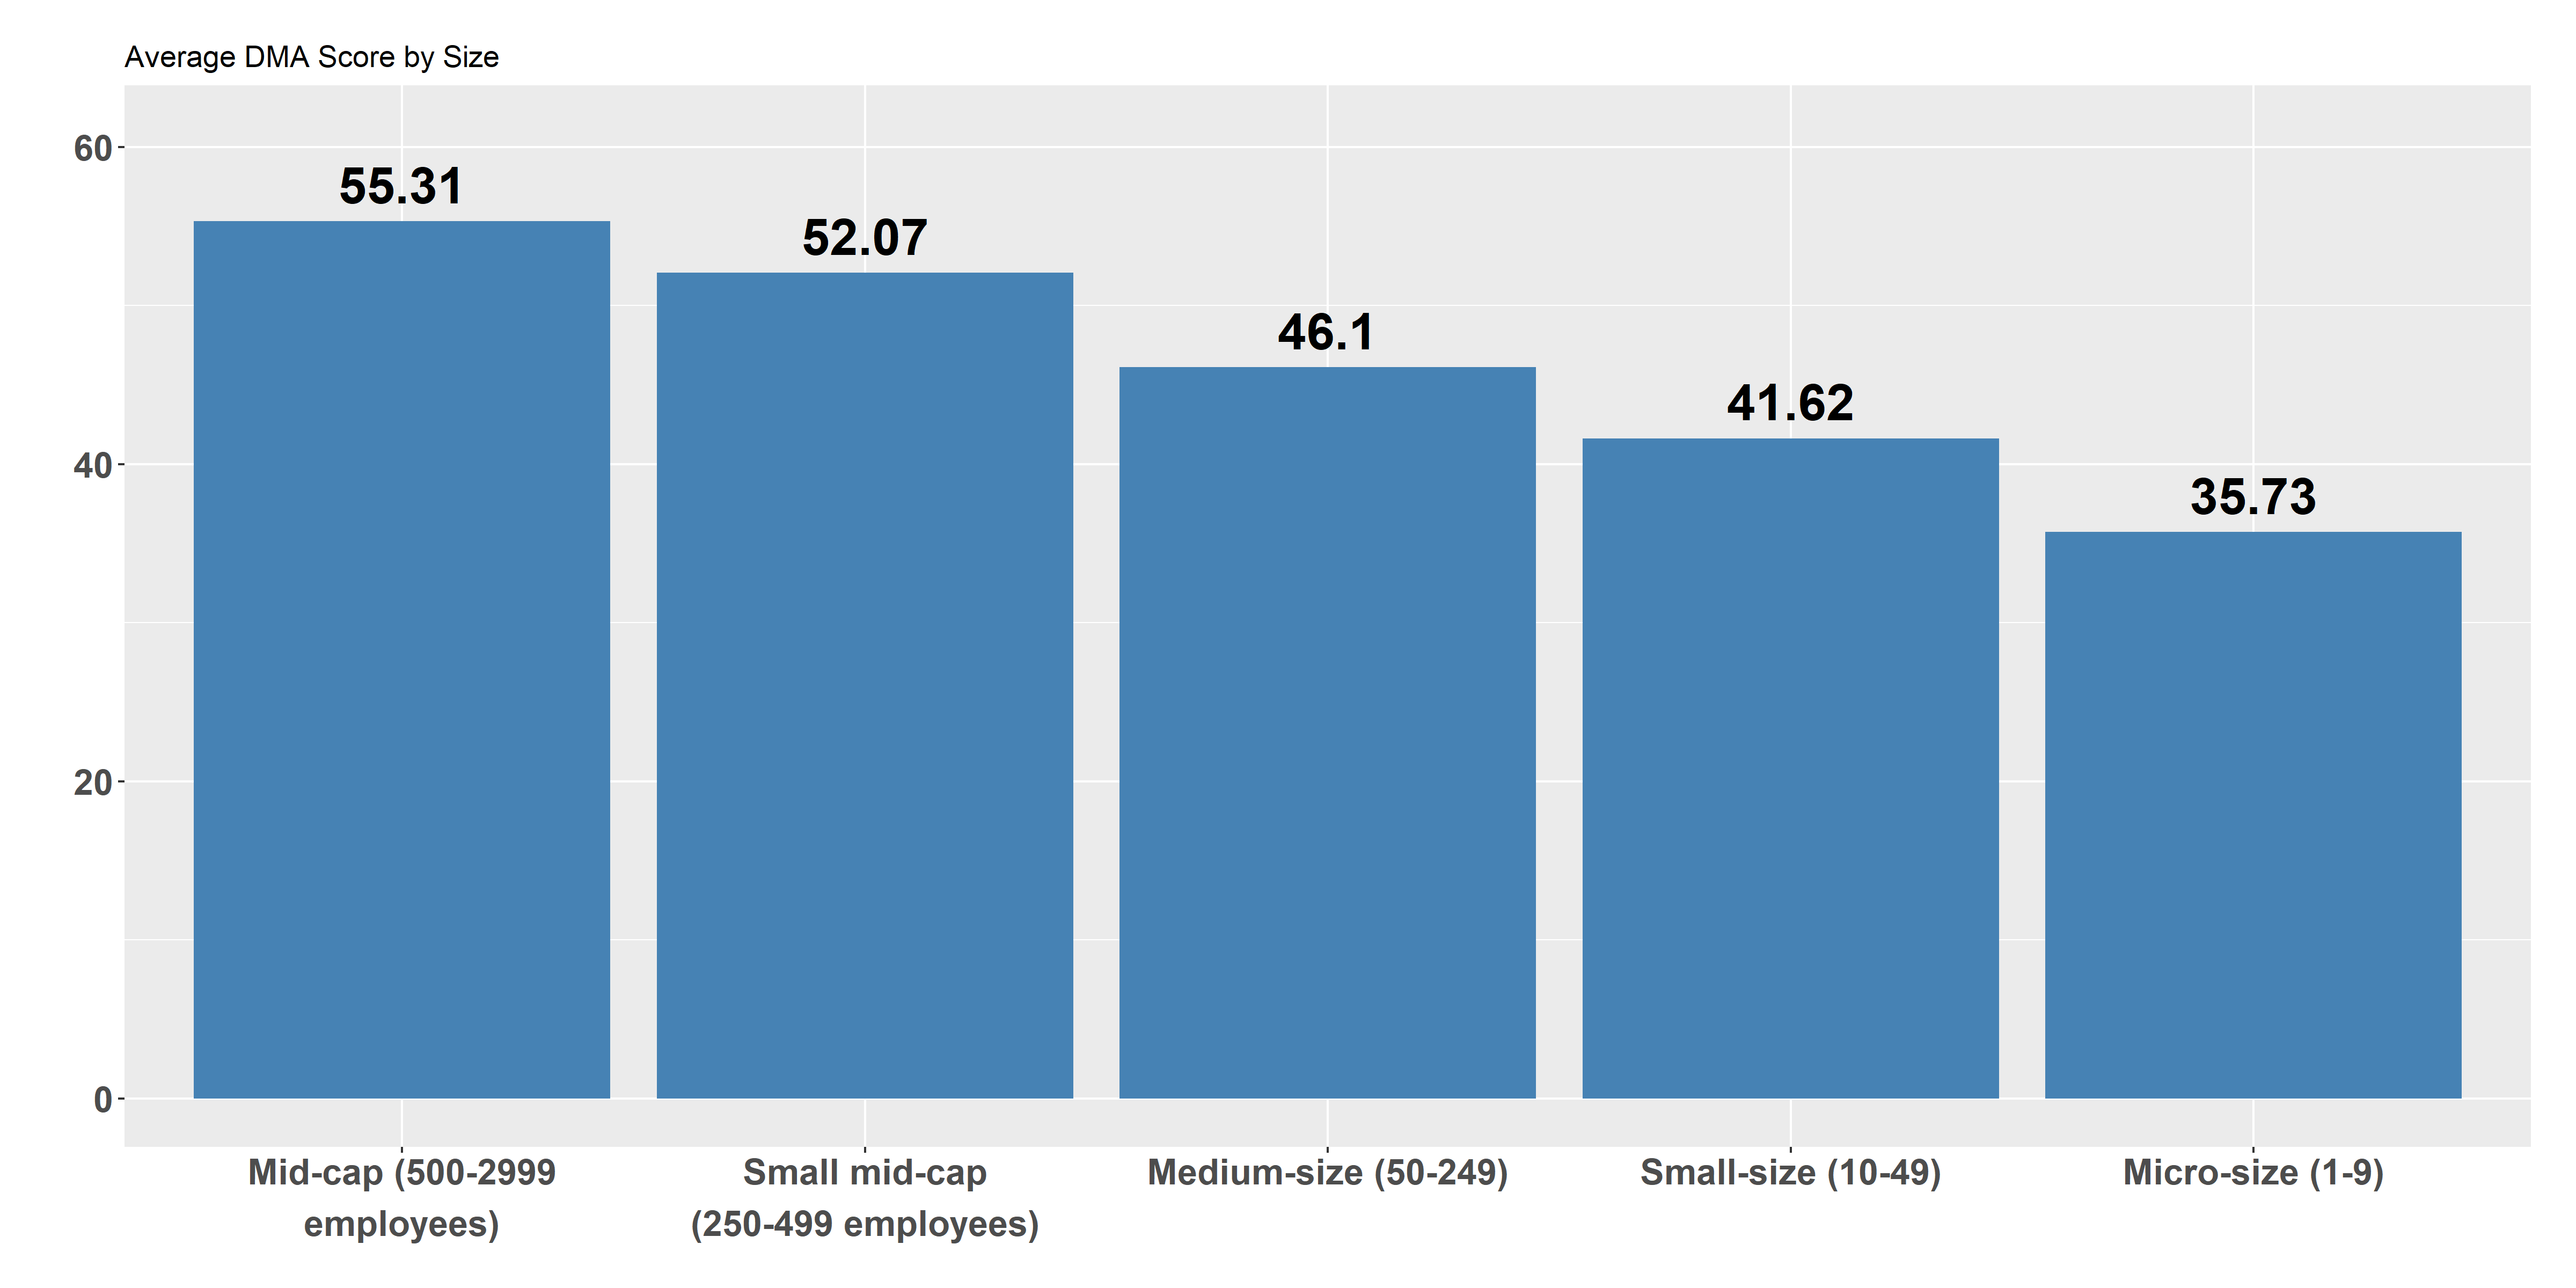
\includegraphics[width=0.6\textheight]{../Output/avg_dmascore_by_size.png}
    \caption{Distribution of the average DMA score across size categories.}
    \label{fig:dma_size_chart}
\end{figure}

\par As you can see in the breakdown by dimension below, the observation of a positive relationship between digital maturity score and size of the firm remains true for each of the six dimensions of the DMA survey. However, we can observe how the drop in average score differs from one dimension to the other. We can also appreciate how, for some of these dimensions, the drop is very steep in the smallest size cathegory, while for others the big decline seems to come before. These observations can help identify points at which size reaches a critical mass and can lead to higher-on-average levels of digital maturity. 


\begin{figure}[p]
    \centering
    \begin{subfigure}[b]{0.48\textwidth}
        \centering
        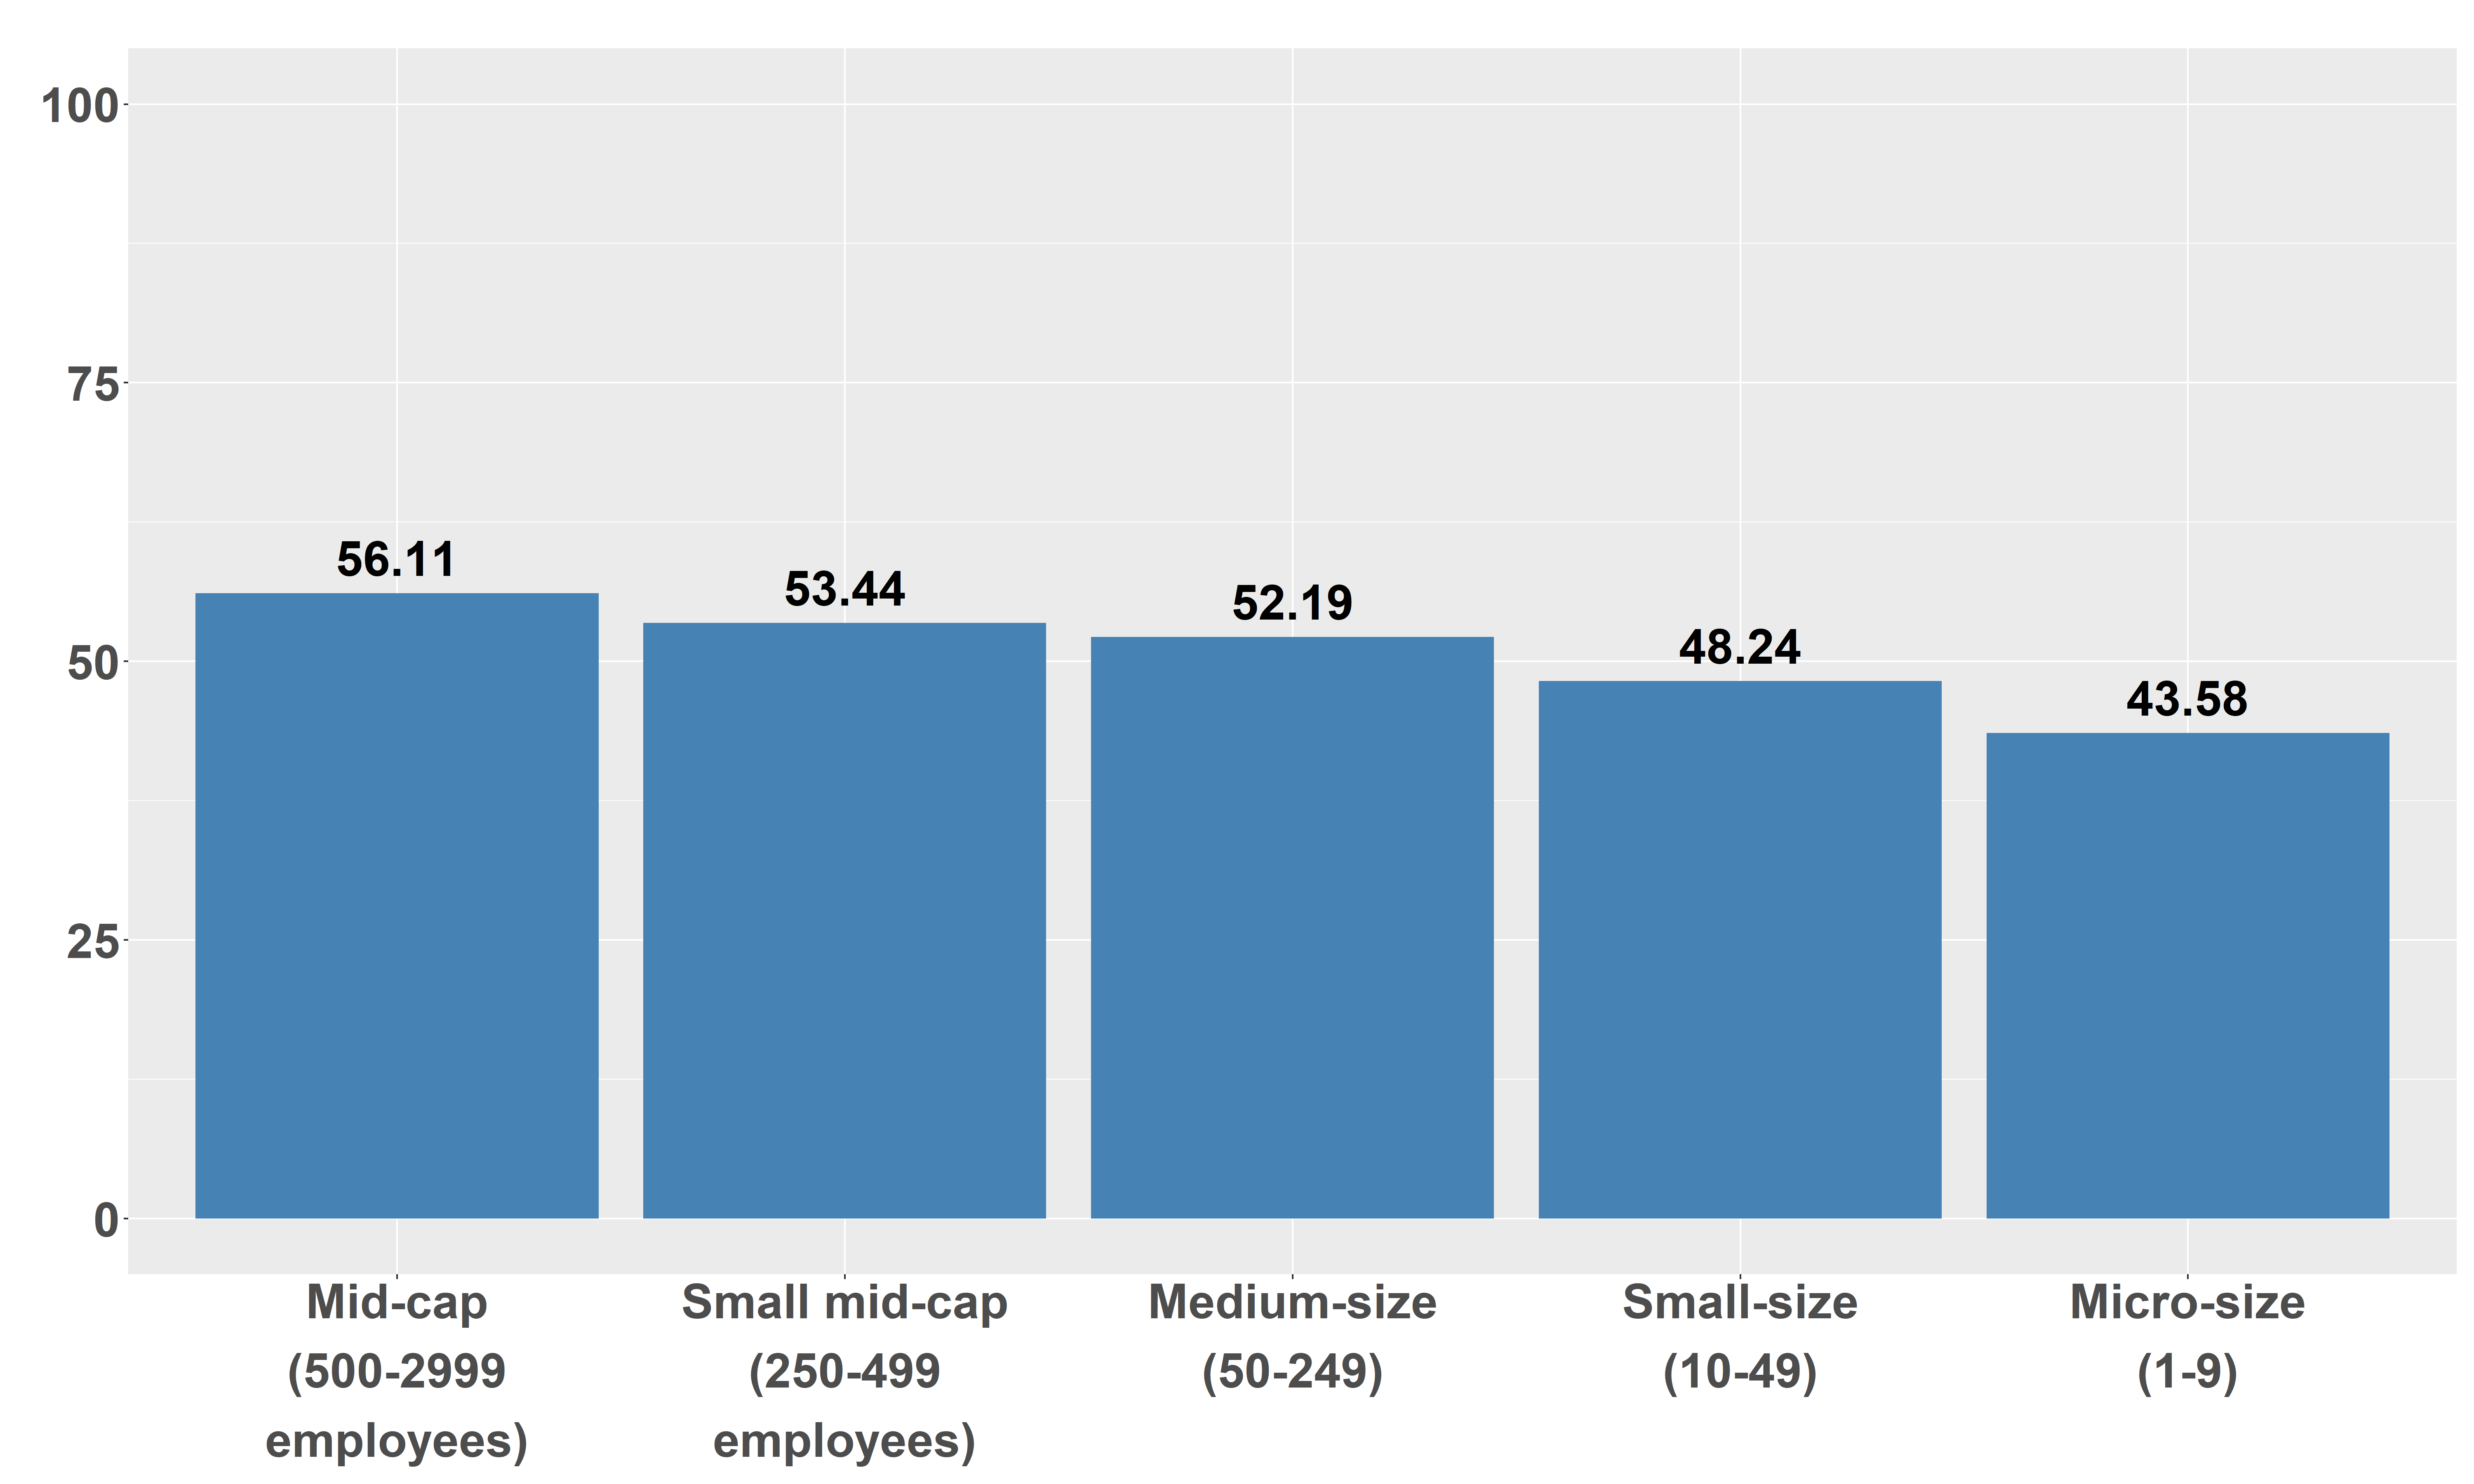
\includegraphics[width=\linewidth]{../Output/avg_dmascore_by_size_dig_business_strat.png}
        \caption{Digital Business Strategy}
        \label{fig:dma_size_digital_business_strategy}
    \end{subfigure}
    \hfill
    \begin{subfigure}[b]{0.48\textwidth}
        \centering
        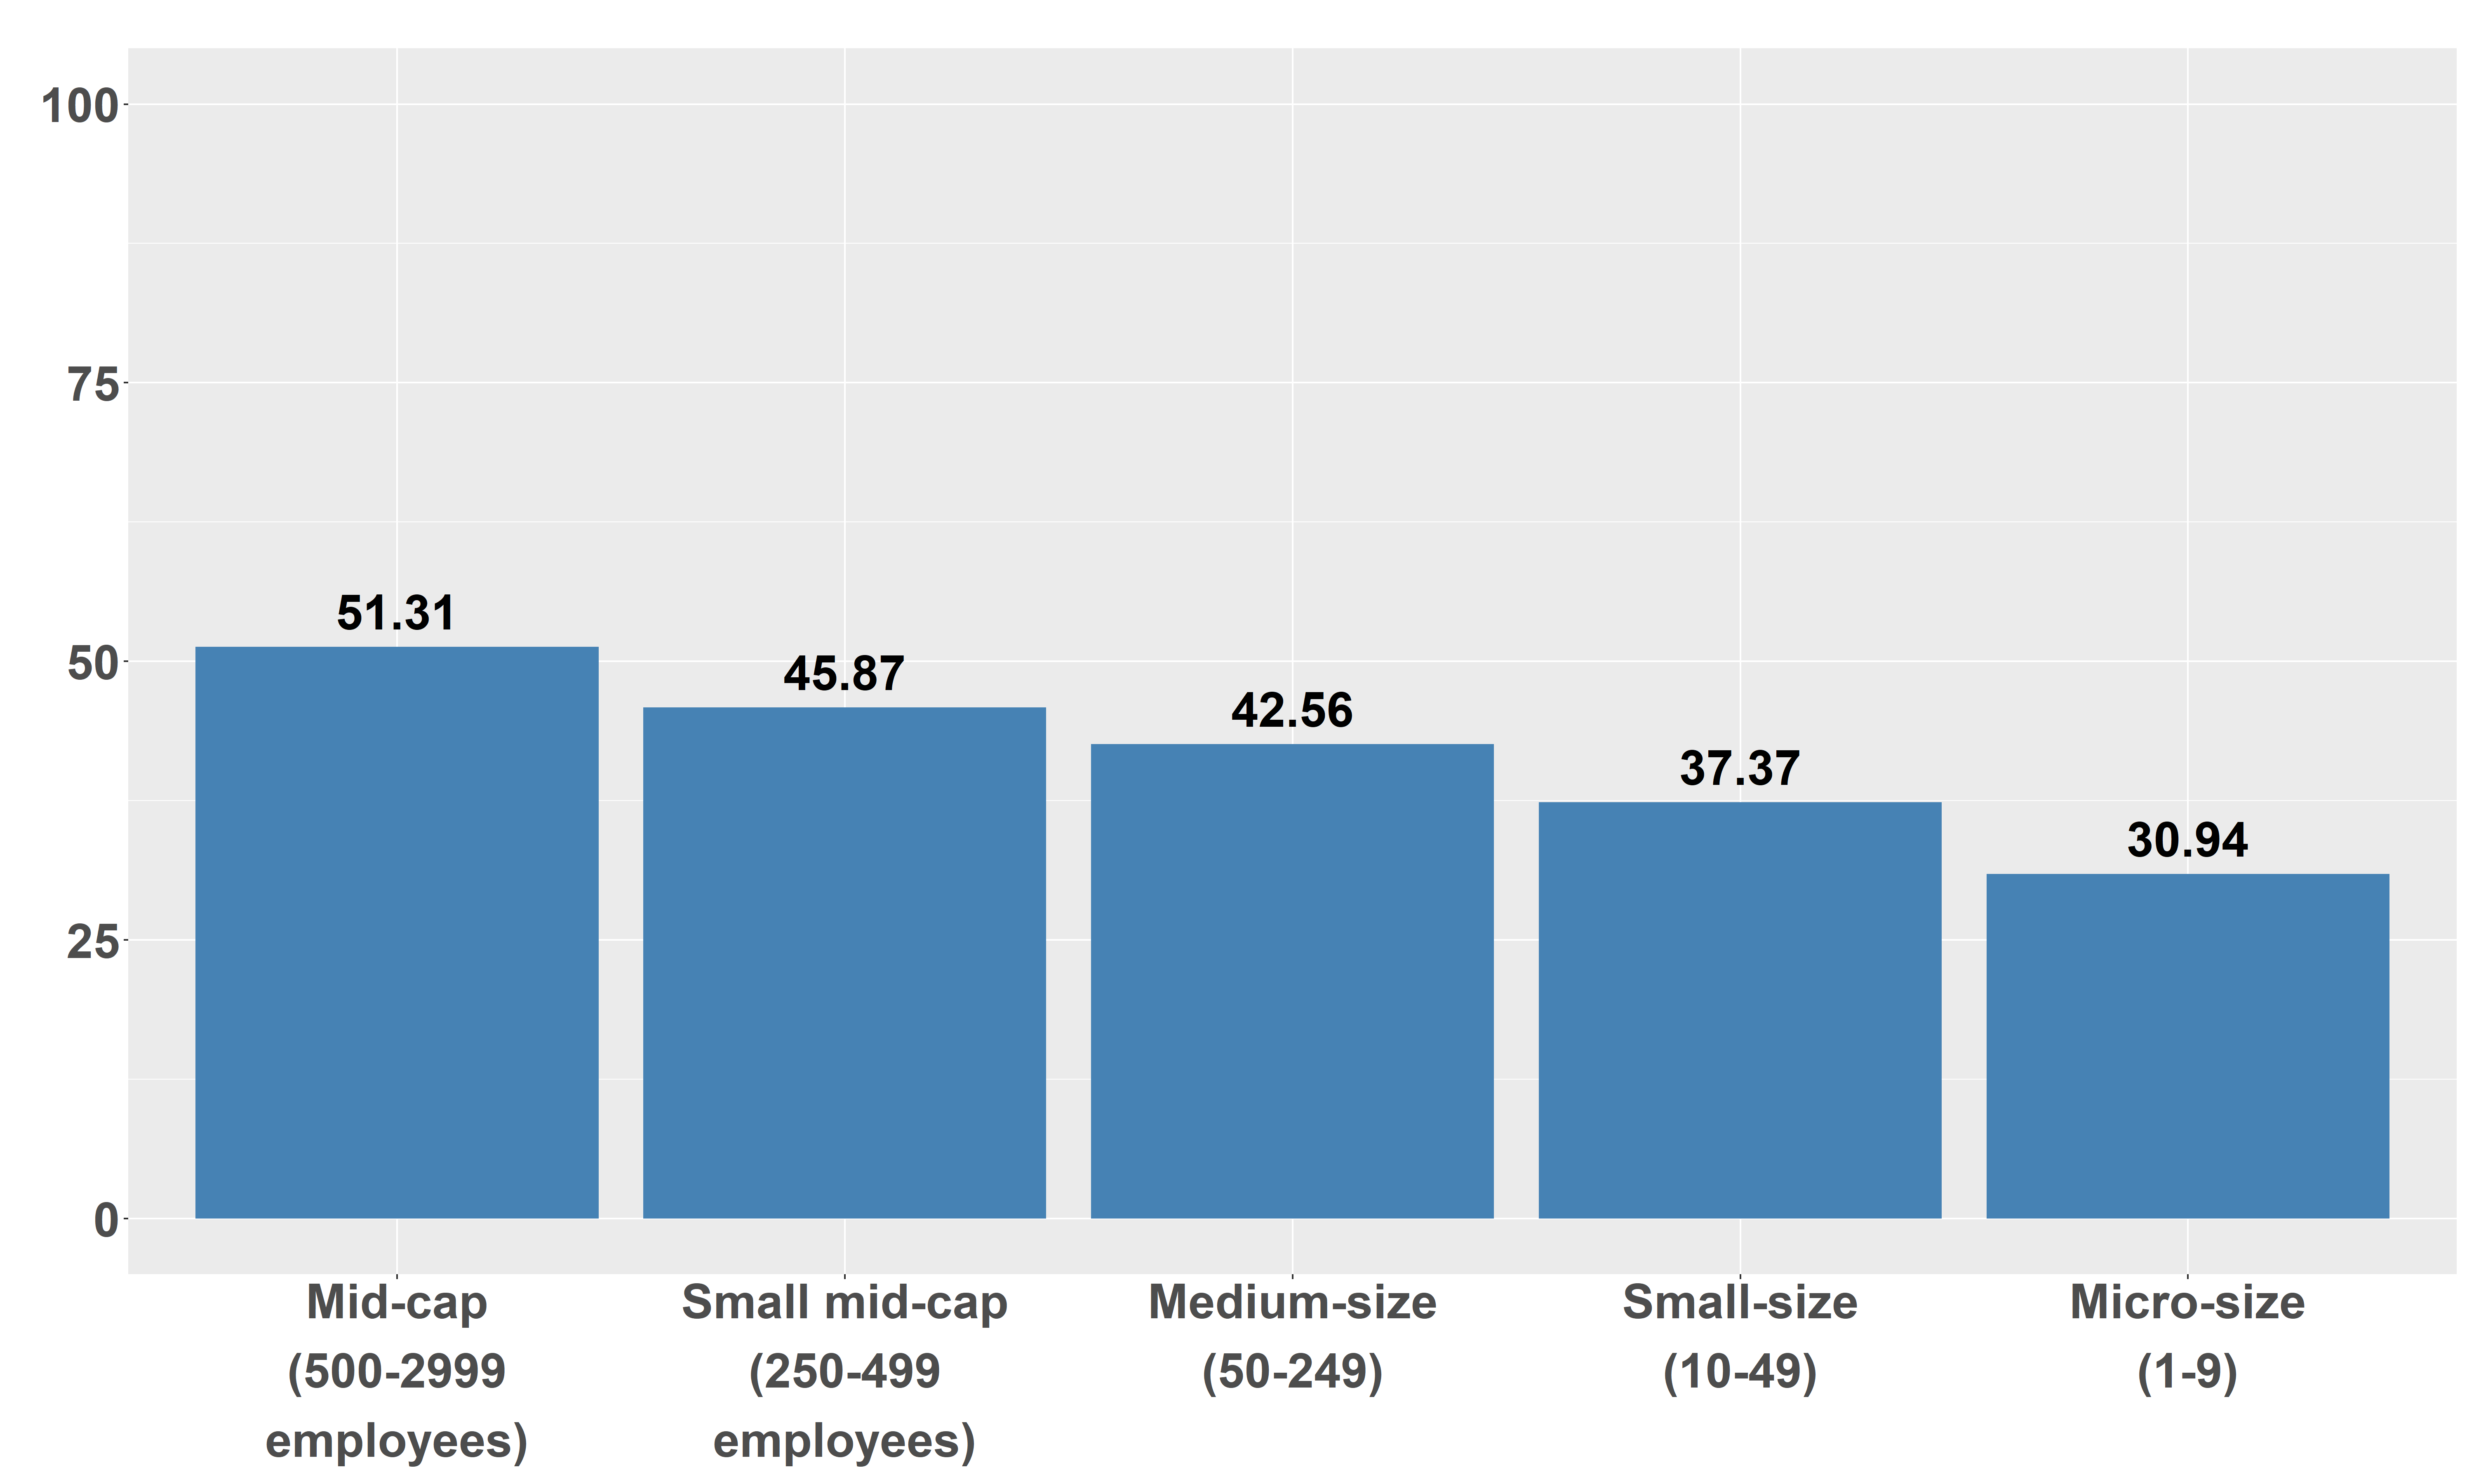
\includegraphics[width=\linewidth]{../Output/avg_dmascore_by_size_dig_readiness.png}
        \caption{Digital Readiness}
        \label{fig:dma_size_digital_readiness}
    \end{subfigure}
    \vfill
    \begin{subfigure}[b]{0.48\textwidth}
        \centering
        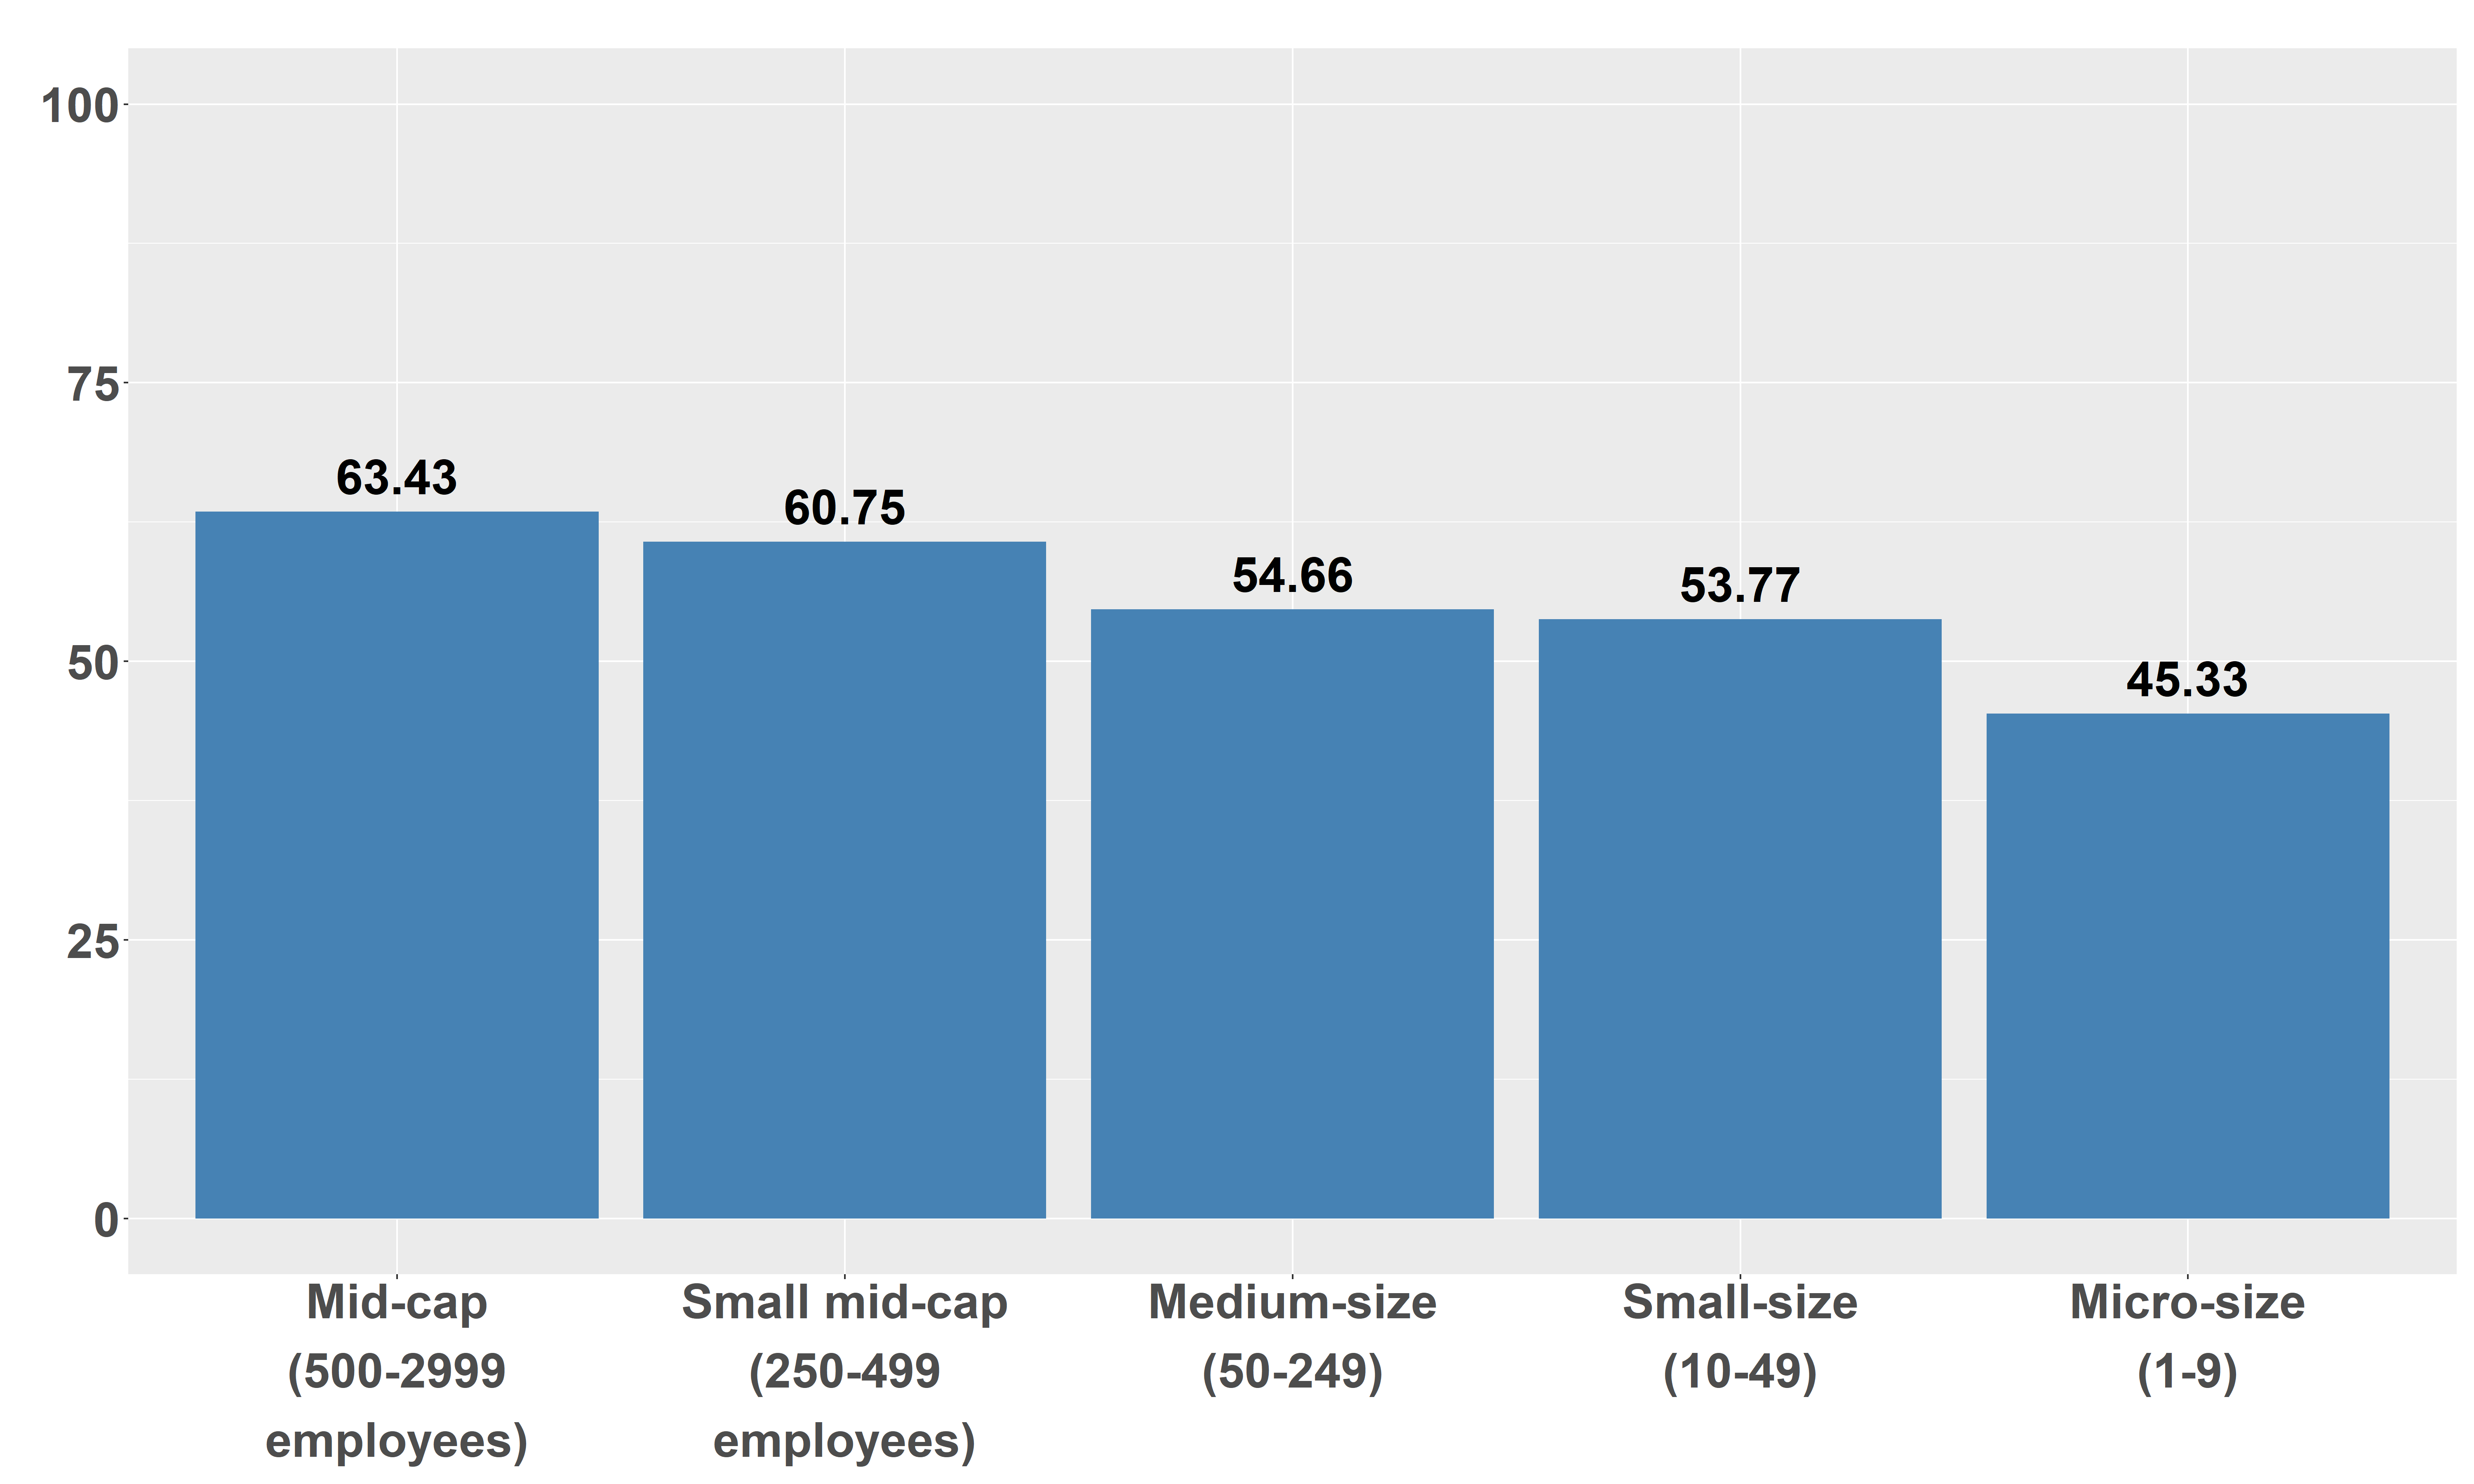
\includegraphics[width=\linewidth]{../Output/avg_dmascore_by_size_hum_centr_dig.png}
        \caption{Human-Centric Digitalization}
        \label{fig:dma_size_human_centric_digitalization}
    \end{subfigure}
    \hfill
    \begin{subfigure}[b]{0.48\textwidth}
        \centering
        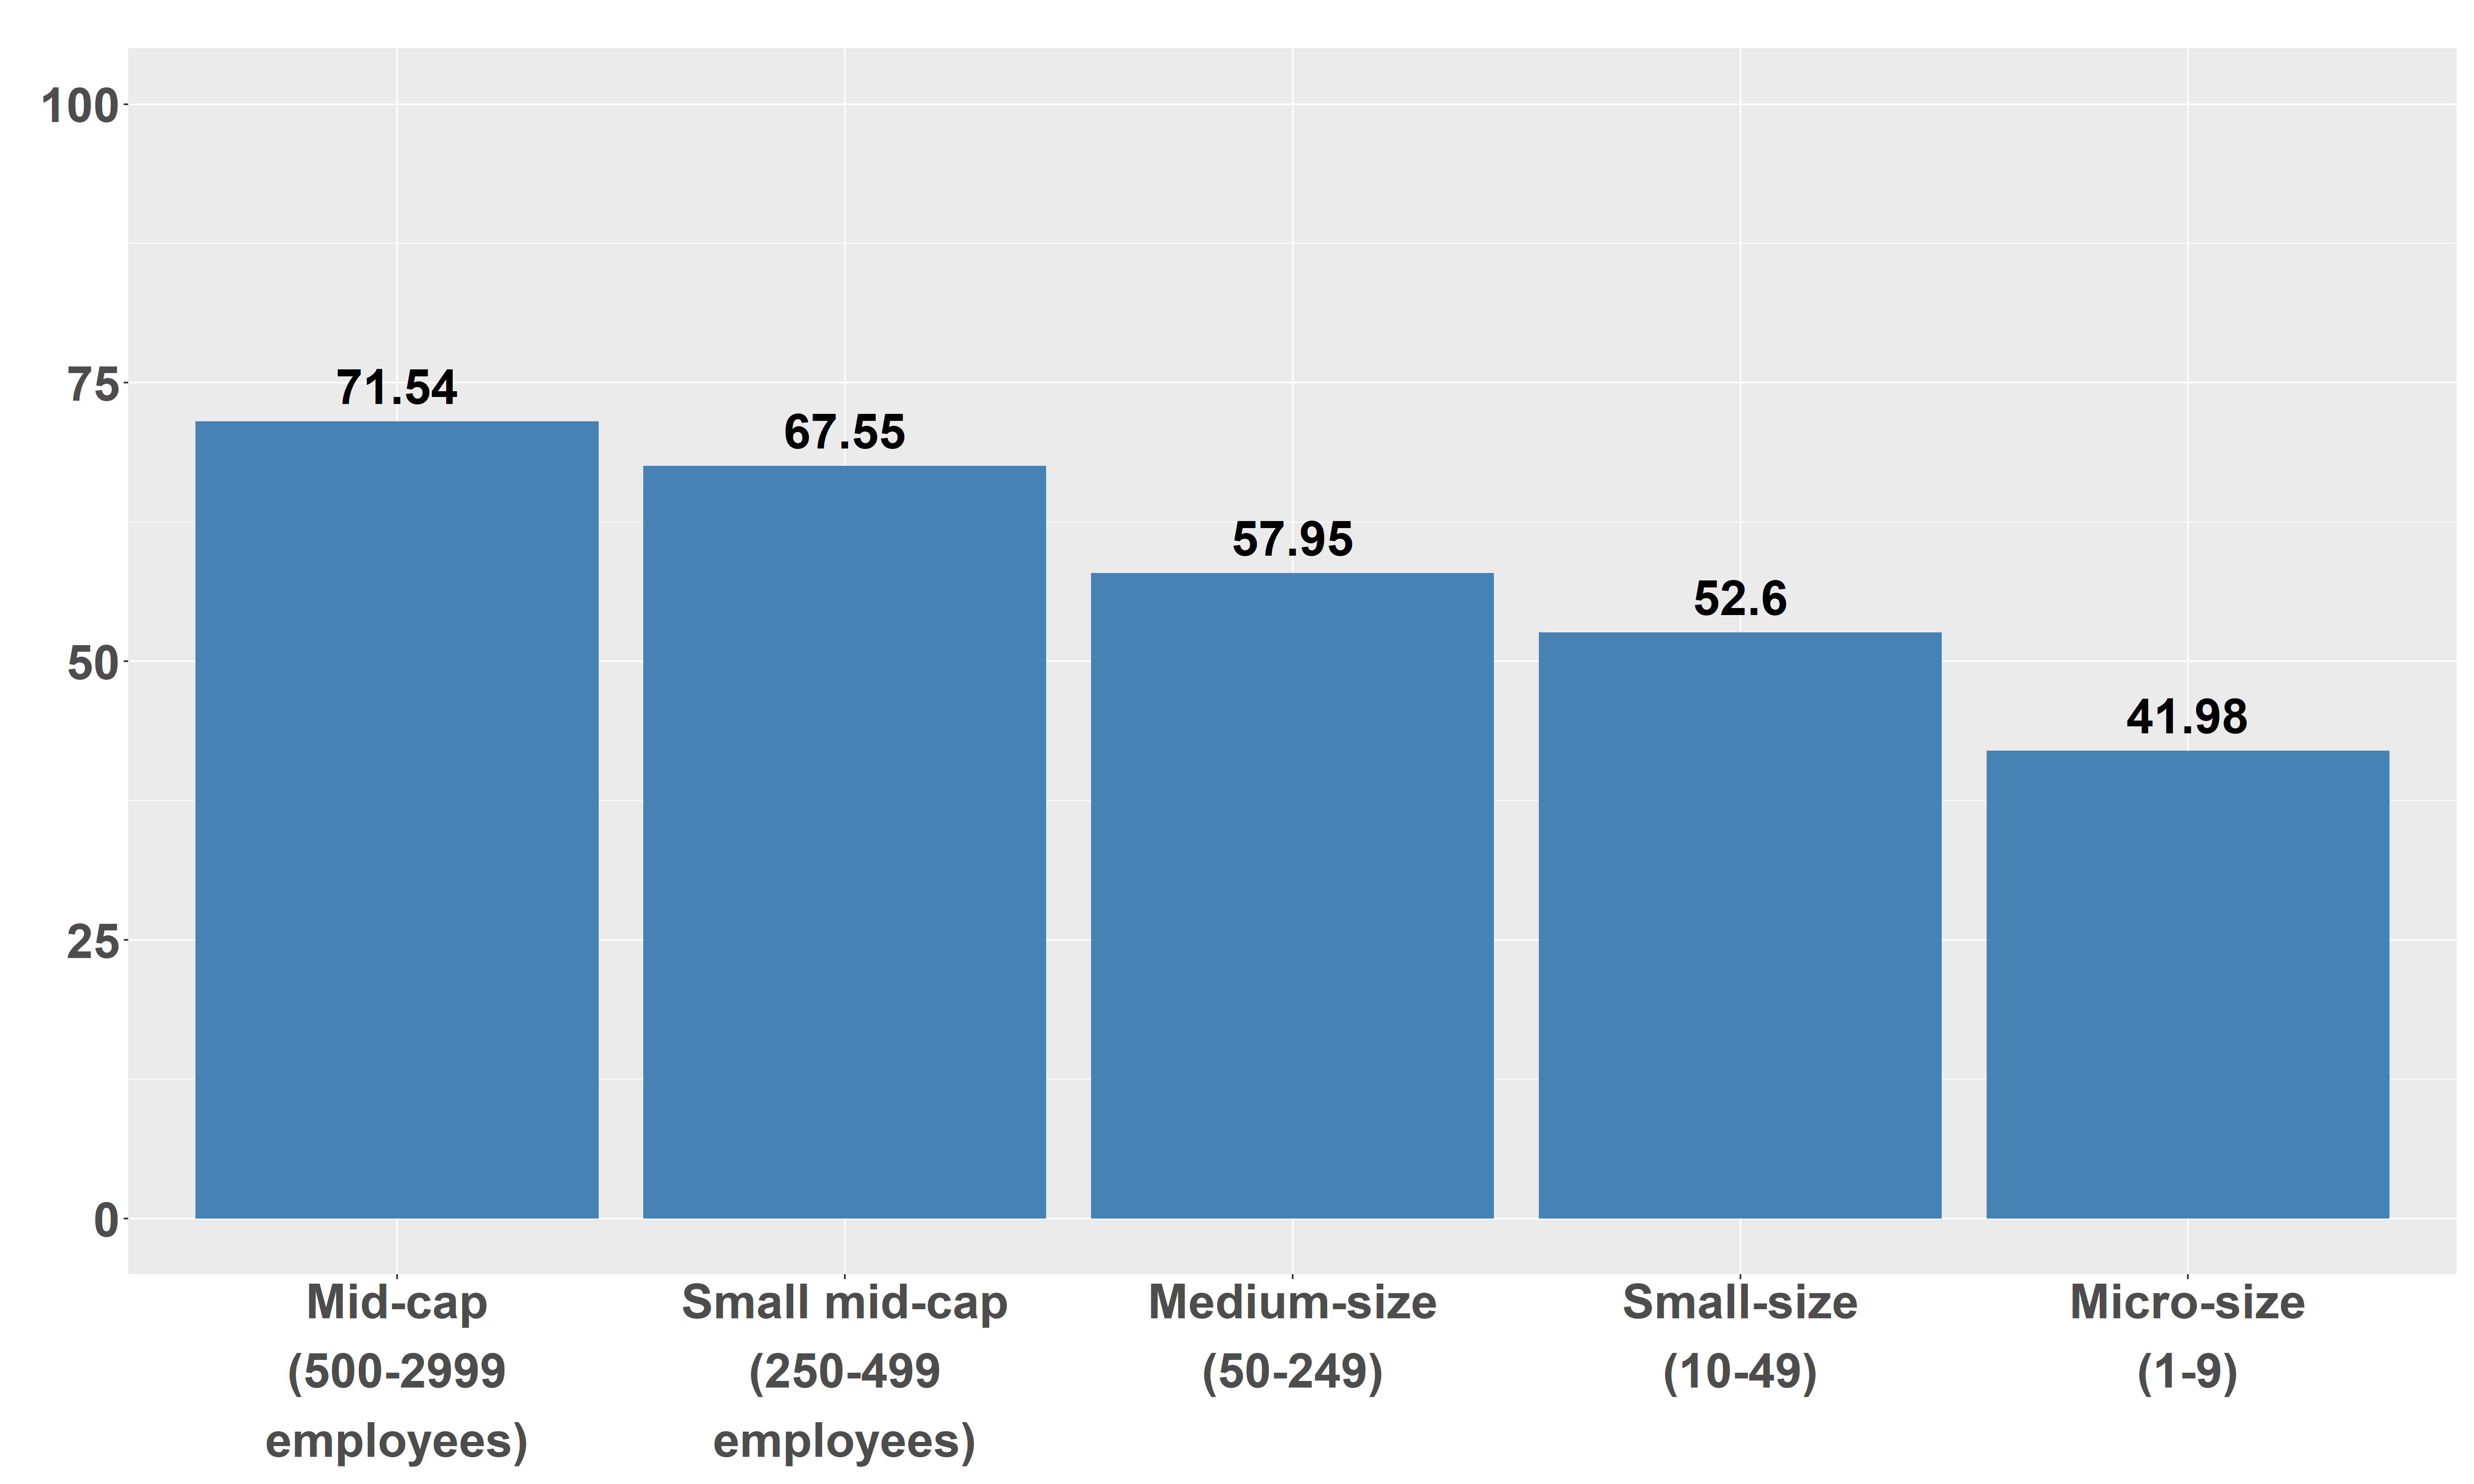
\includegraphics[width=\linewidth]{../Output/avg_dmascore_by_size_data_gov.png}
        \caption{Data Management}
        \label{fig:dma_size_data_management}
    \end{subfigure}
    \vfill
    \begin{subfigure}[b]{0.48\textwidth}
        \centering
        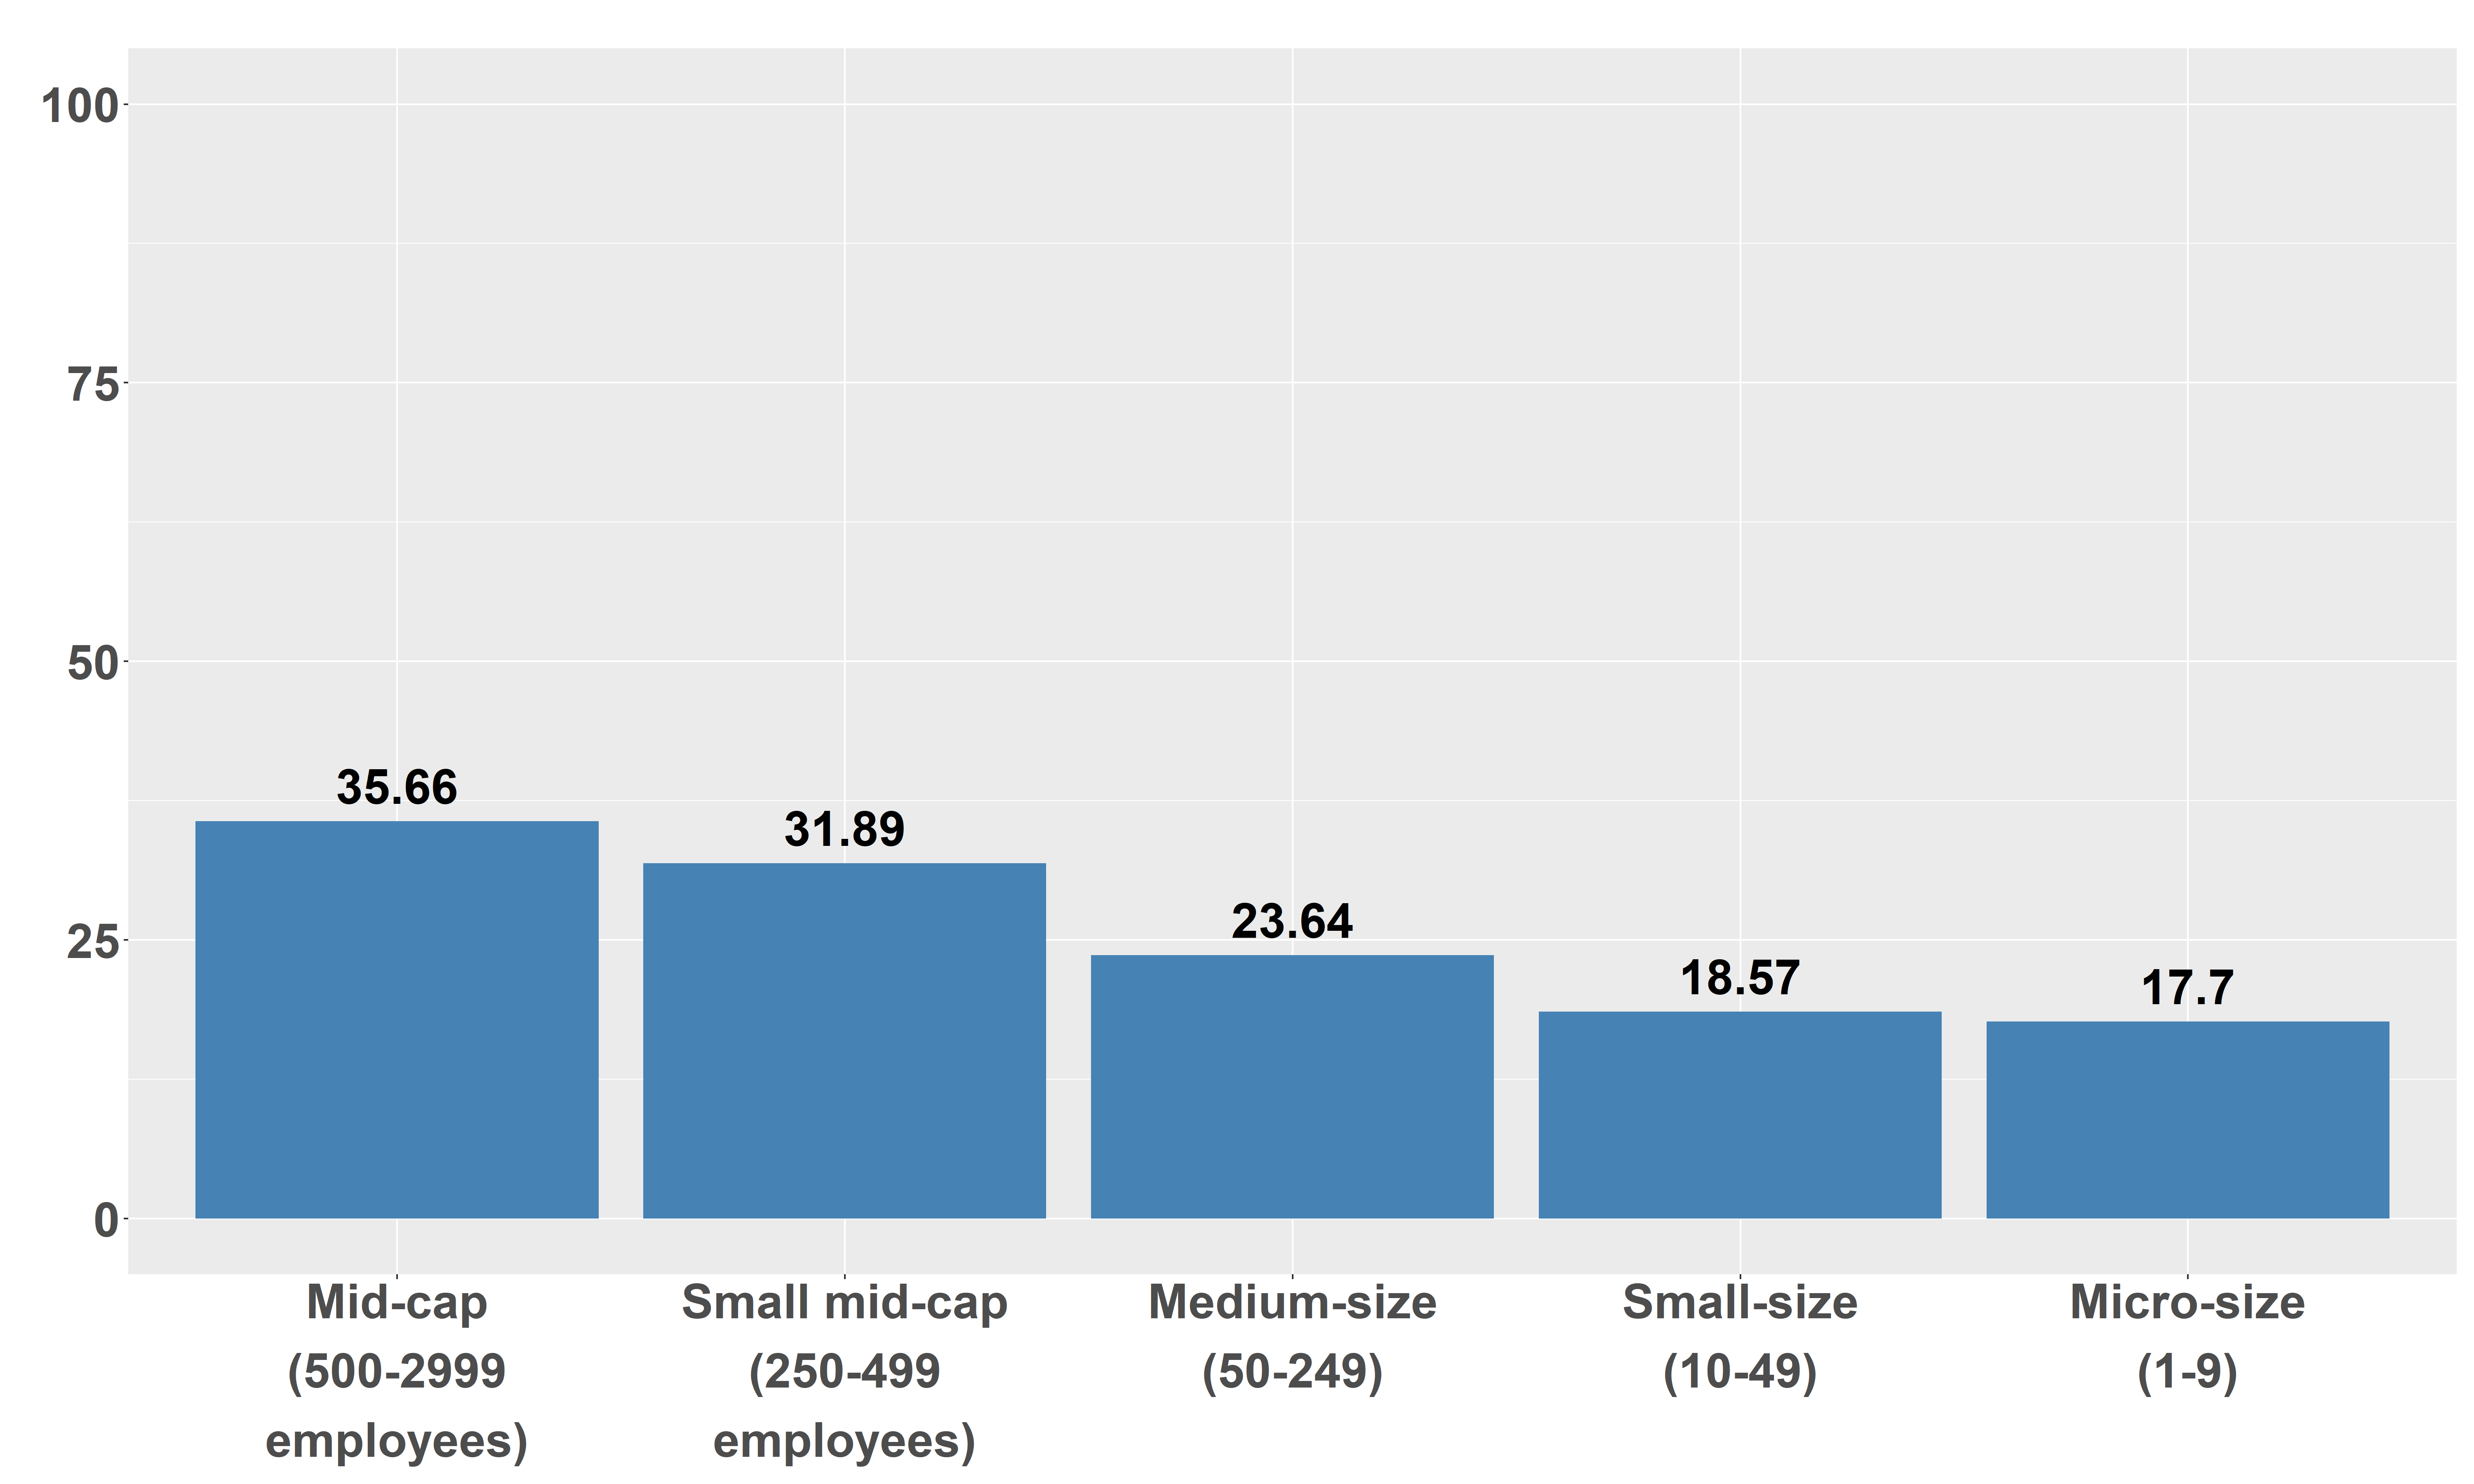
\includegraphics[width=\linewidth]{../Output/avg_dmascore_by_size_automation_ai.png}
        \caption{Automation \& Intelligence}
        \label{fig:dma_size_automation_intelligence}
    \end{subfigure}
    \hfill
    \begin{subfigure}[b]{0.48\textwidth}
        \centering
        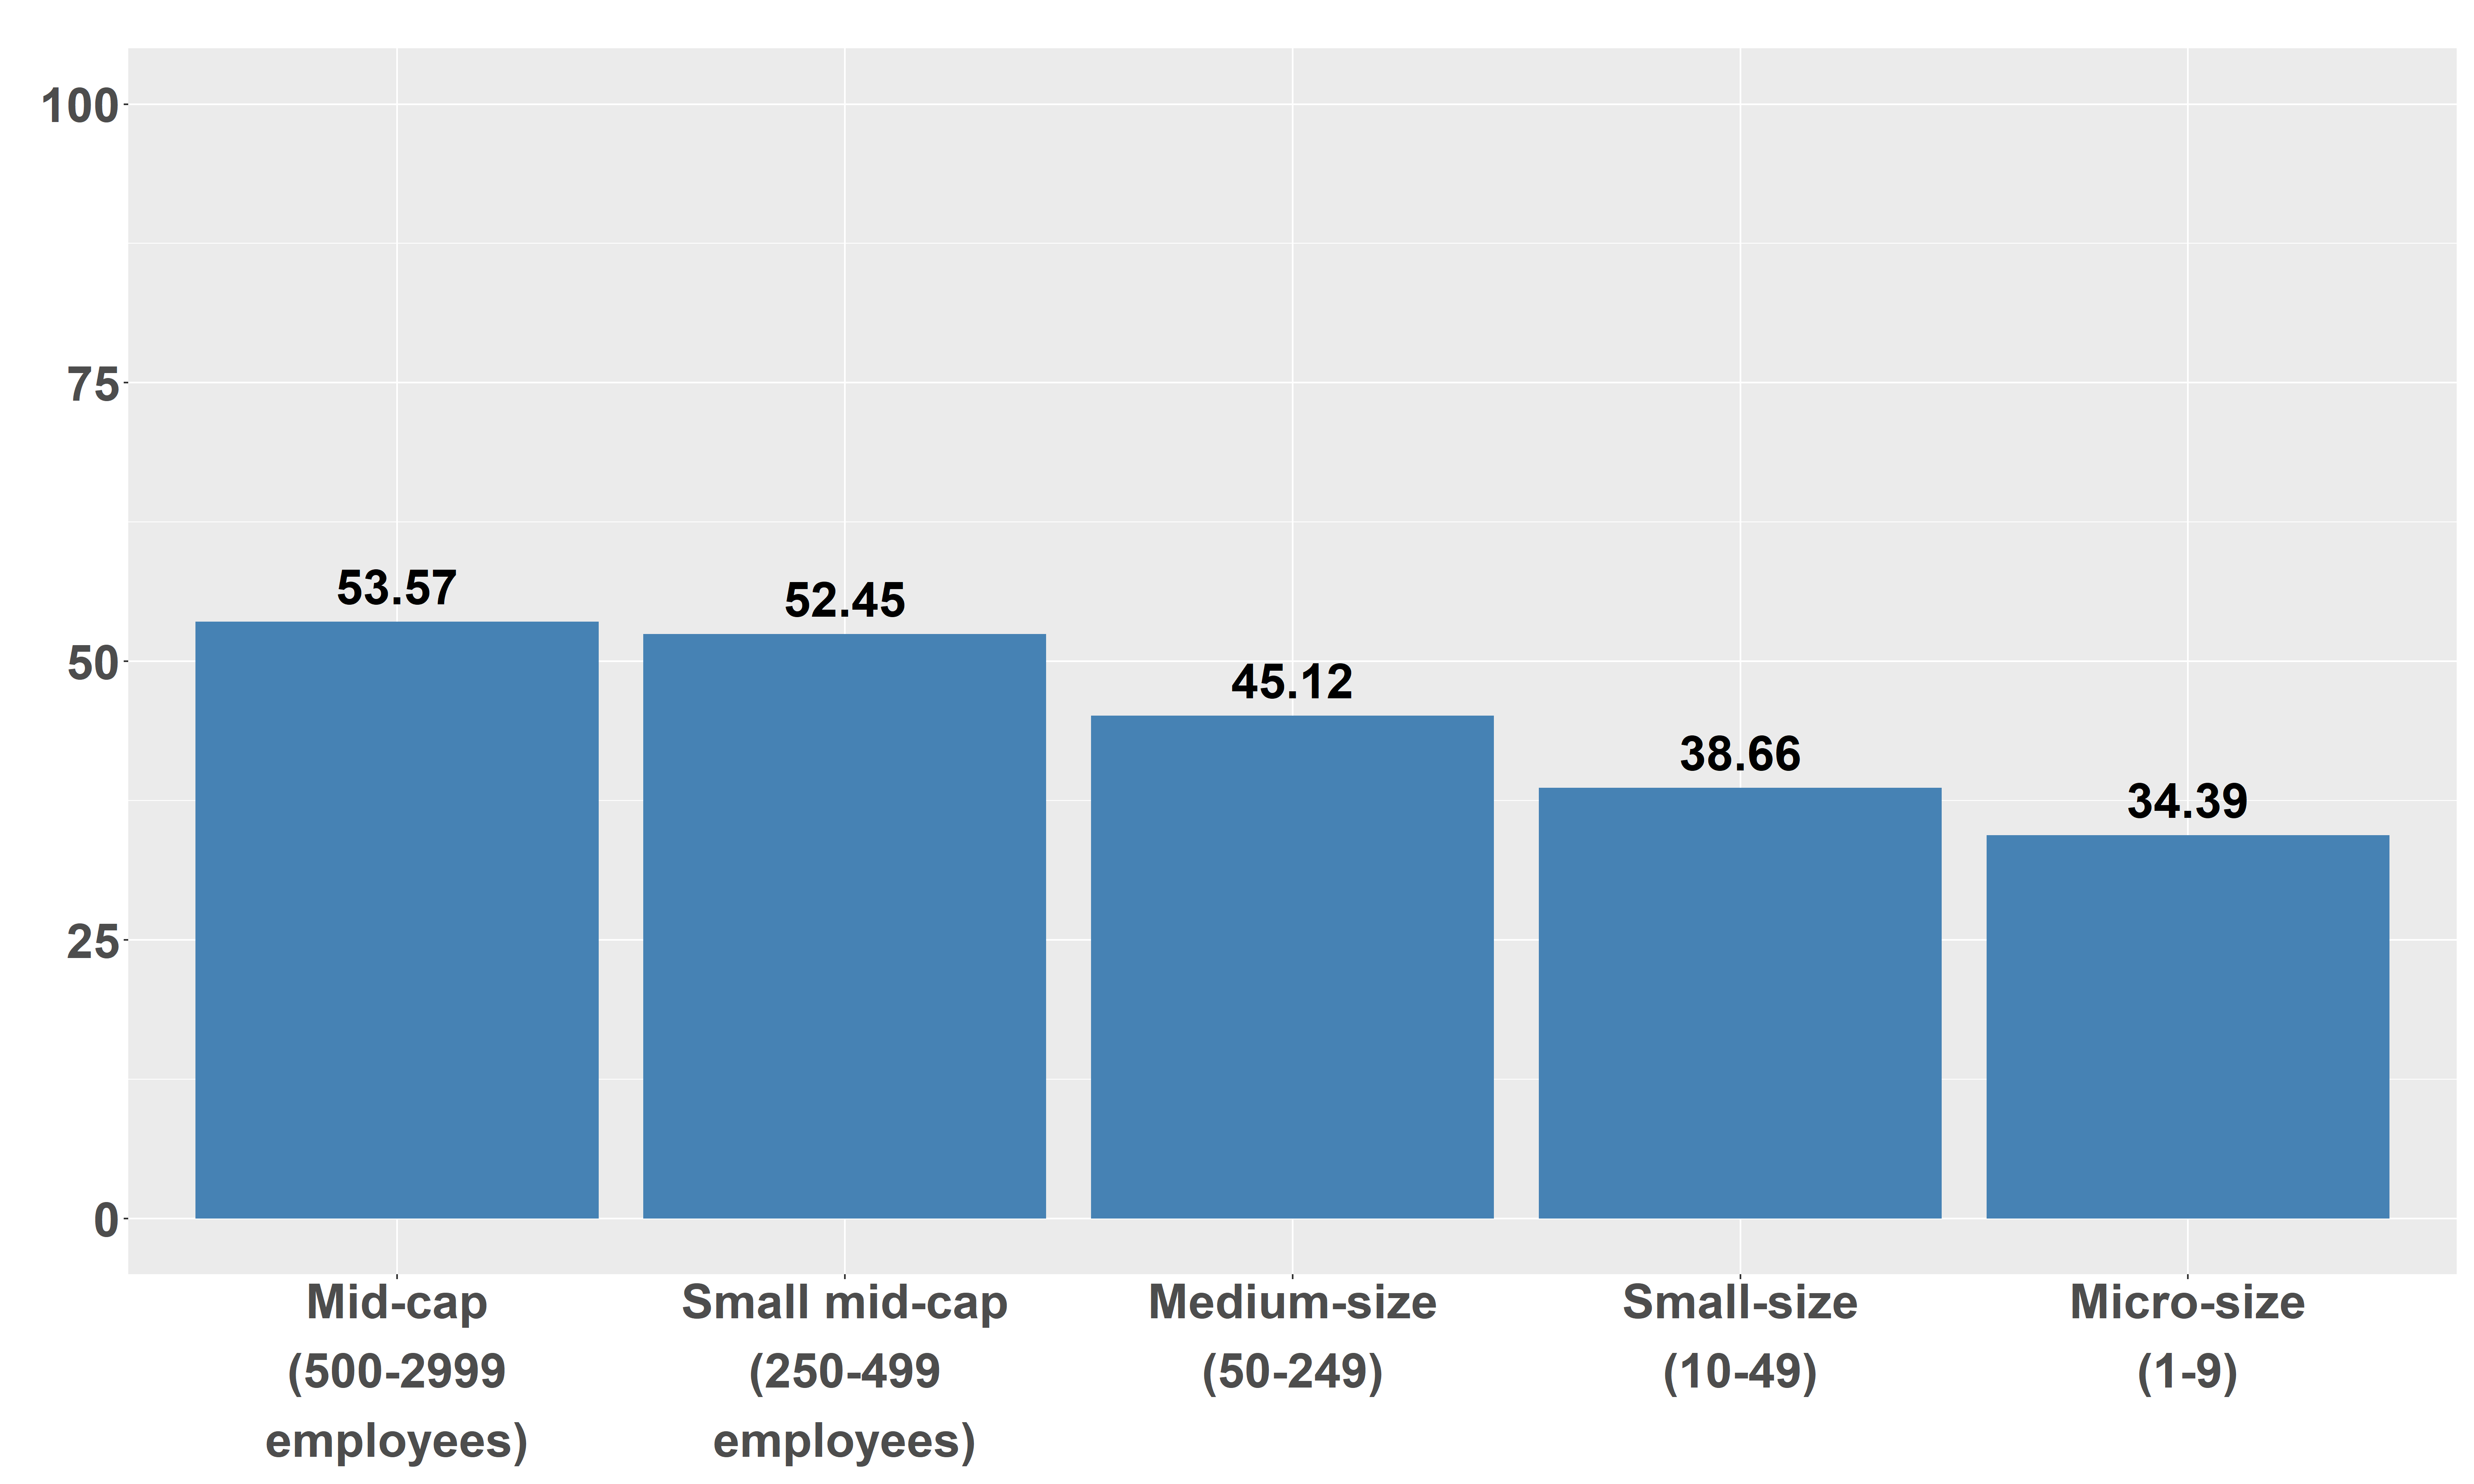
\includegraphics[width=\linewidth]{../Output/avg_dmascore_by_size_green_dig.png}
        \caption{Green Digitalization}
        \label{fig:dma_size_green_digitalization}
    \end{subfigure}
    \caption{\centering{Distribution of the average DMA score across size categories for each of the six DMA dimensions.}}
    \label{fig:dma_size_all}
\end{figure}


\par For example, if we look at the human-centric digitalization dimension, we see how there is not a huge difference in average score in the brackets going from 10 up to 249 employees, while micro-firms under 10 employees present an 8.5 point drop in average score. This suggests that the incredibly limited dimension of these firms does not allow them to invest in their staff, thus damaging the dimension's score.


\par Something similar can be said for the Automation \& Intelligence dimension, although with a difference. In this case, every size category actually struggles with the adoption of this type of advanced technologies. The largest firms have an average score of only 35.66 in this dimension. This is probably due to the fact that most of the large firms in the EU are active in mature sectors of the industry. Thus, they are less innovative and present lower levels of advanced technology adoption with respect to counterparts belonging to newer sectors of the economy. However, here we see that the score is consistently low in the first two categories, suggesting that a certain critical mass is needed for this dimension to improve in a measurable way. If this is the case, we should not expect to see a large increase in this indicator for small and micro firms when looking at $T1$ observations, unless firms do actually grow very rapidly.




\par We can now move on to examine some insights obtained from the analysis of the firms' replies to the questions in the DMA survey. Specifically, one of the most interesting things we can look at is the current uptake in specific technologies. To this end, I will not present the responses to every question (you can find them in the Appendix); instead, I will present the responses from the questions belonging to the Digital Readiness, Data Management, and Automation \& Intelligence dimensions.

\par Starting with Digital Readiness, we can see the breakdown of survey responses from its first subdimension, related to Basic Digital Technologies, in the image below.
\begin{figure}[h!]
    \centering
    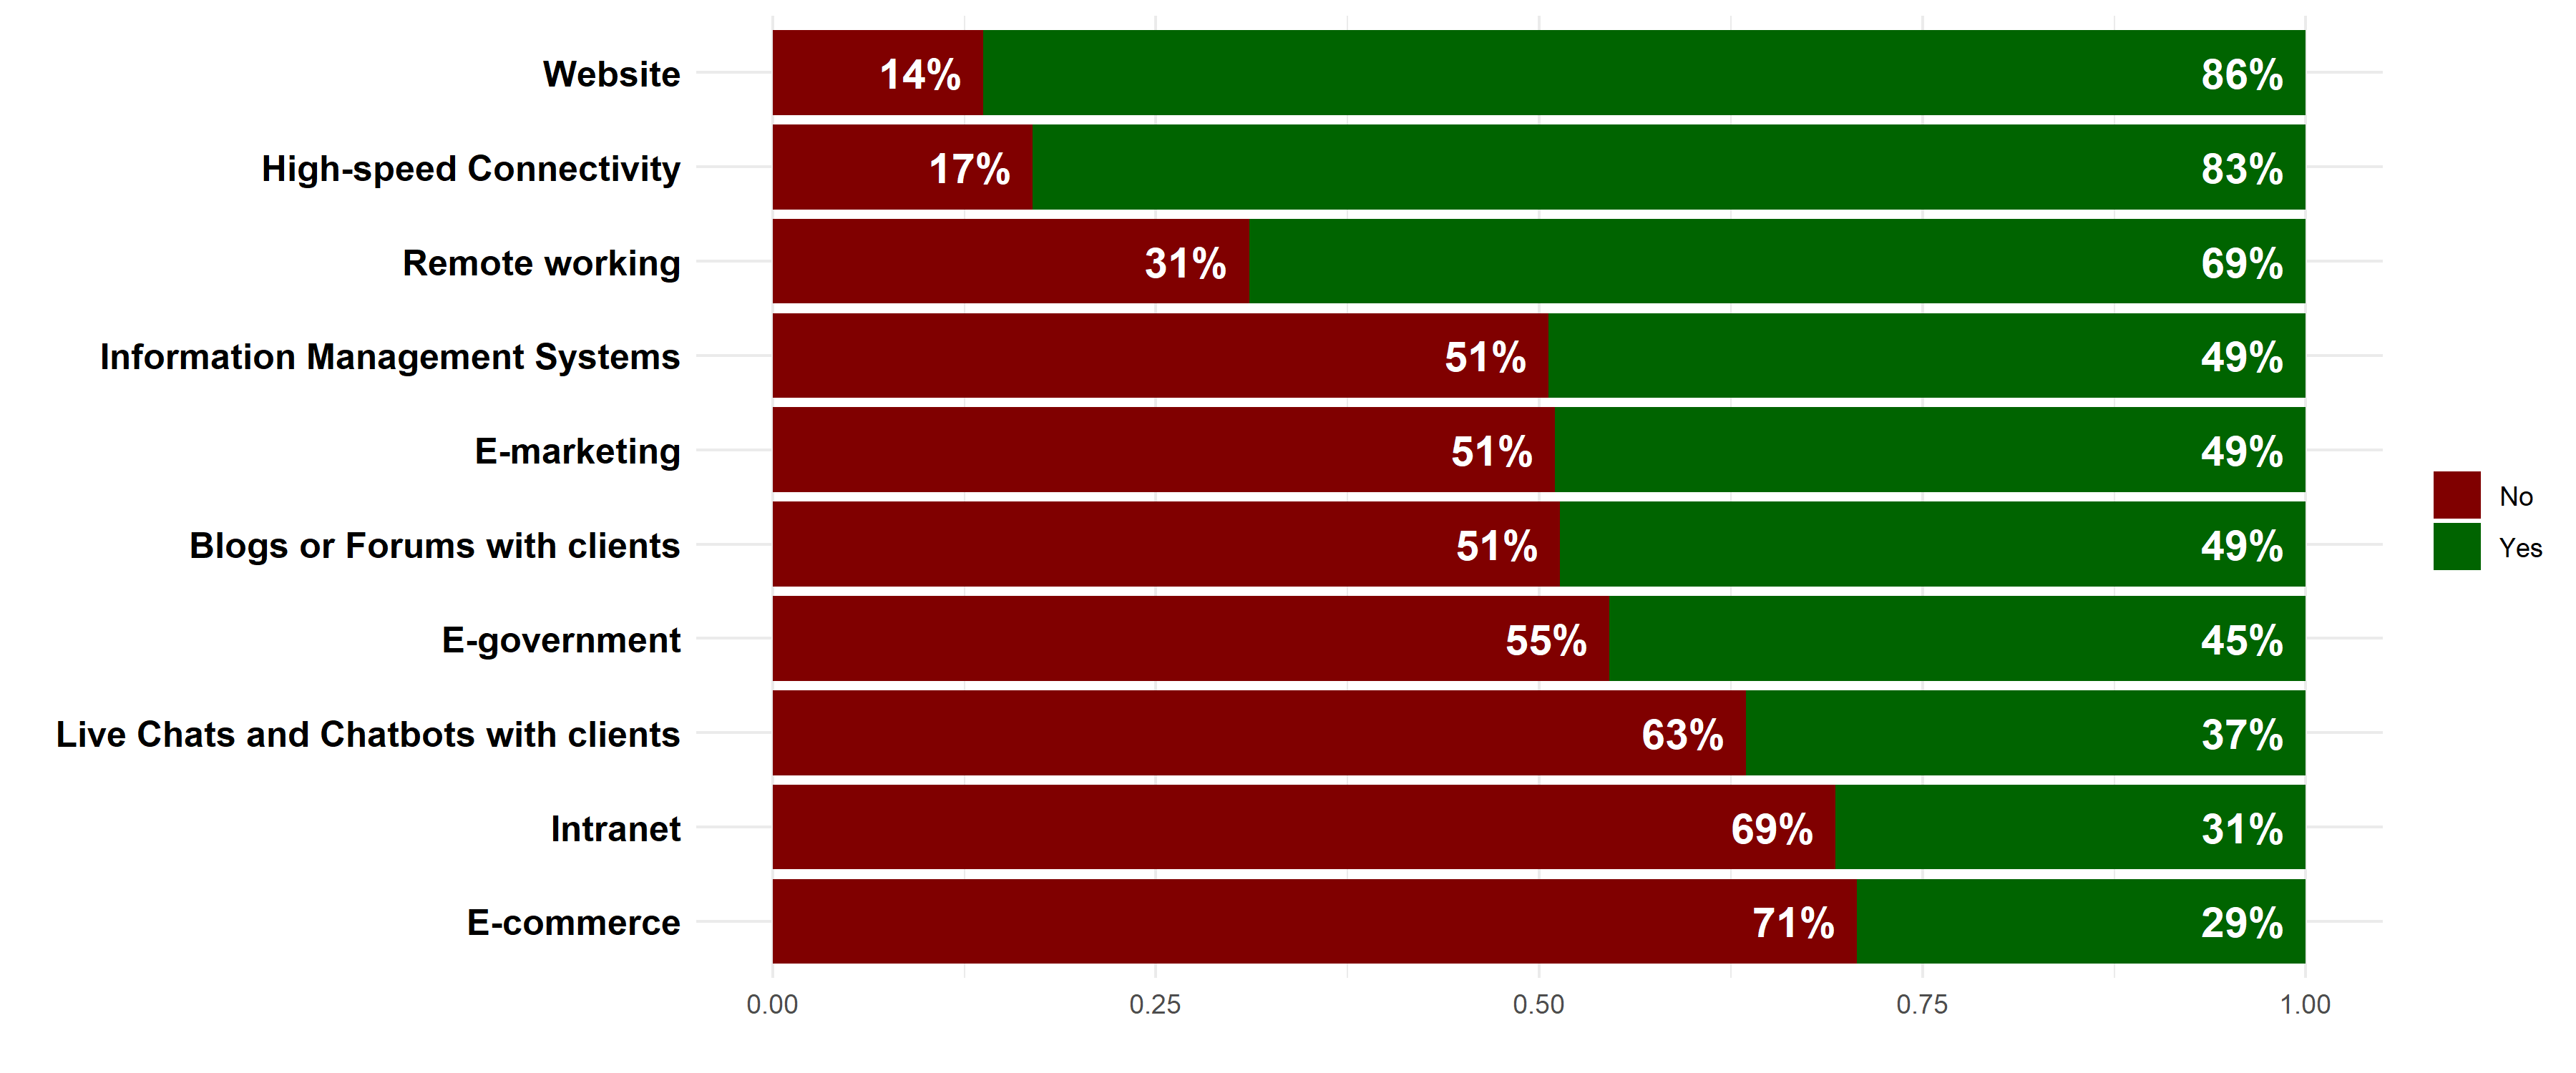
\includegraphics[width=\linewidth]{../Output/q3.png}
    \caption{\centering{Breakdown of responses to Question 3 of the DMA survey, part of the Digital Readiness dimension.}}
    \label{fig:q3_table}
\end{figure}

\par Items are ordered from the most widely adopted to the least widely adopted. Right away, we can see how almost all of the surveyed firms have an online website, and high-speed internet connectivity. Almost 70\% of firms report to utilize remote working for their operations: the significant amount of firms giving remote working as an option is probably due to the teleworking policies put in place during the Covid-19 pandemic.
Another interesting item is Intranet; only 31\% of firms report to have an intranet; however, this is probably due to the fact that most firms in the sample are small or even micro enterprises. Lastly, we can notice how few firms utilize e-commerces: however, this is probably a consequence of the sample being made mostly by manufacturing firms, and not by firms in the retail sector.

\par Let's move on to the subdimension on Advanced Digital Technologies. In this case, respondents are not restricted to a Yes/No response. In fact, they can choose the option that most accurately represents the level at which that technology is implemented in the firm. The levels from which respondents can choose are: Not Used, Consider to use, Prototyping, Testing, Implementing, and Operational.

\par The added granularity of the information in this case can help us identify which technologies are deemed interesting, even if not yet operational. Also, this subdimension in the future can be useful to determine if the declared path on which the firm's technology adoption process was set has become reality or not.

\begin{figure}[h!]
    \centering
    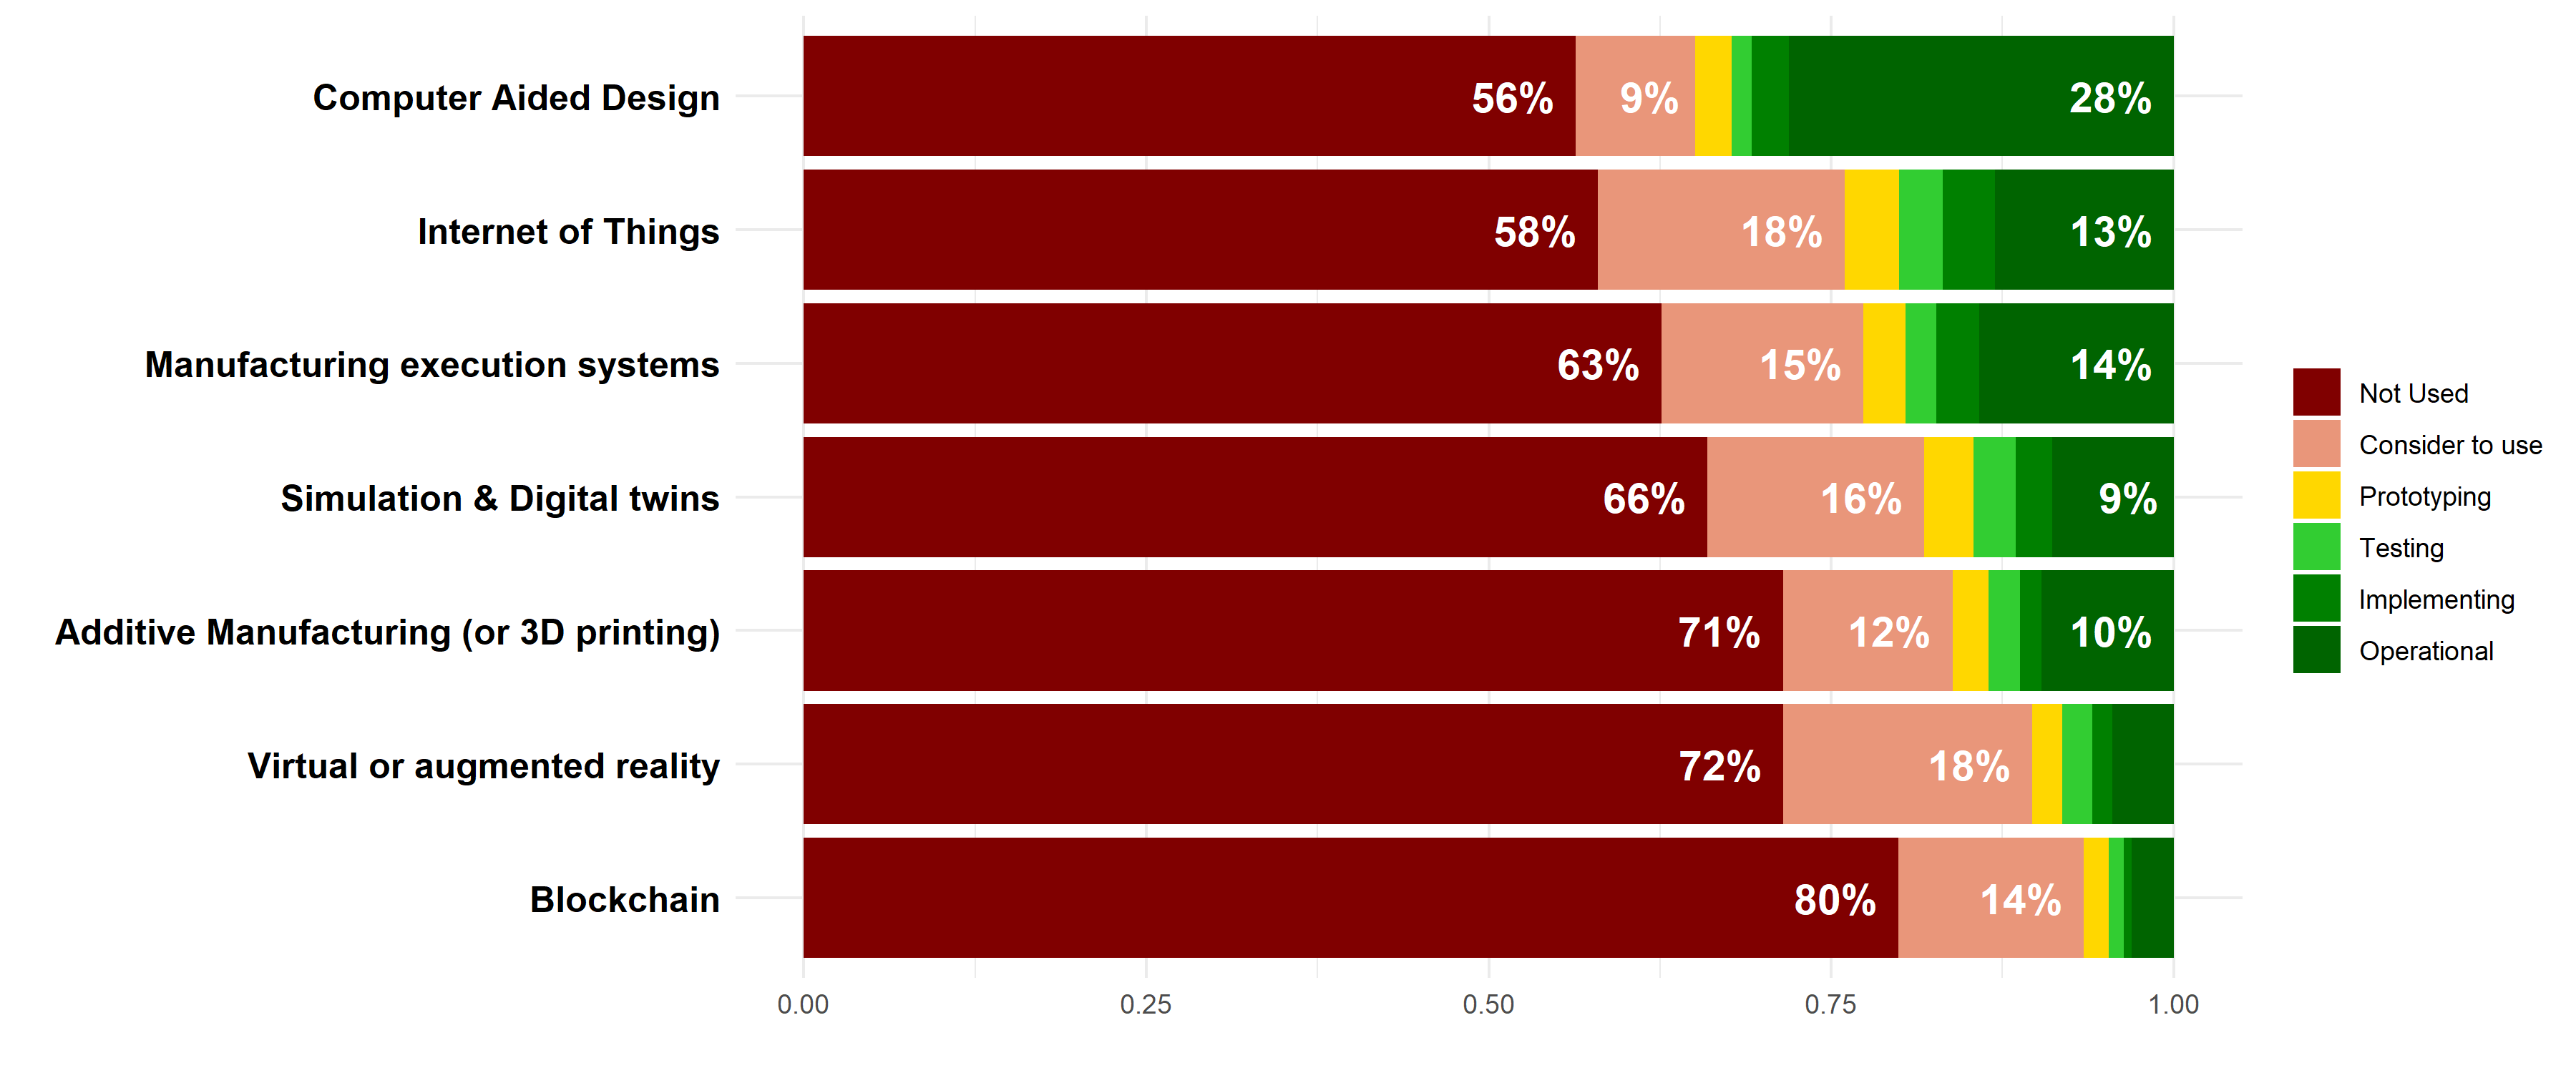
\includegraphics[width=\linewidth]{../Output/q4.png}
    \caption{\centering{Breakdown of responses to Question 4 of the DMA survey, part of the Digital Readiness dimension.}}
    \label{fig:q4_table}
\end{figure}

\par What we can see for now in the breakdown of survey responses is how most of the advanced digital technologies surveyed are not used at all. Actually, none of the technologies presented would be adopted by a majority of firms even if all declared plans to adopt them were to succeed. This is probably an indication of how few firms actually appreciate the potential positive impact these technologies can have on their operations. This should be an aspect to be checked when $T1$ observation start coming in relevant numbers. At that point, we would see if any firm has changed their views after the EDIH intervention. If for example we see that on average more firms are taking into consideration the idea of adopting these advanced digital technologies, then we would have indication of the program working as intended. Even more positive would be if we got data confirming that technology adoption plans are proceeding, thus getting higher proportions for the "Implementing" and "Operational" response options.

\par Let's now consider survey responses coming from the Data Management dimension. This dimension of the survey is important to understand how firms deal with internal data as well as data coming from their customers. The first question in the Data Management dimensions asks firms "How is your enterprise data managed (i.e. stored, organised, accessed and exploited)?"

\begin{figure}[h!]
    \centering
    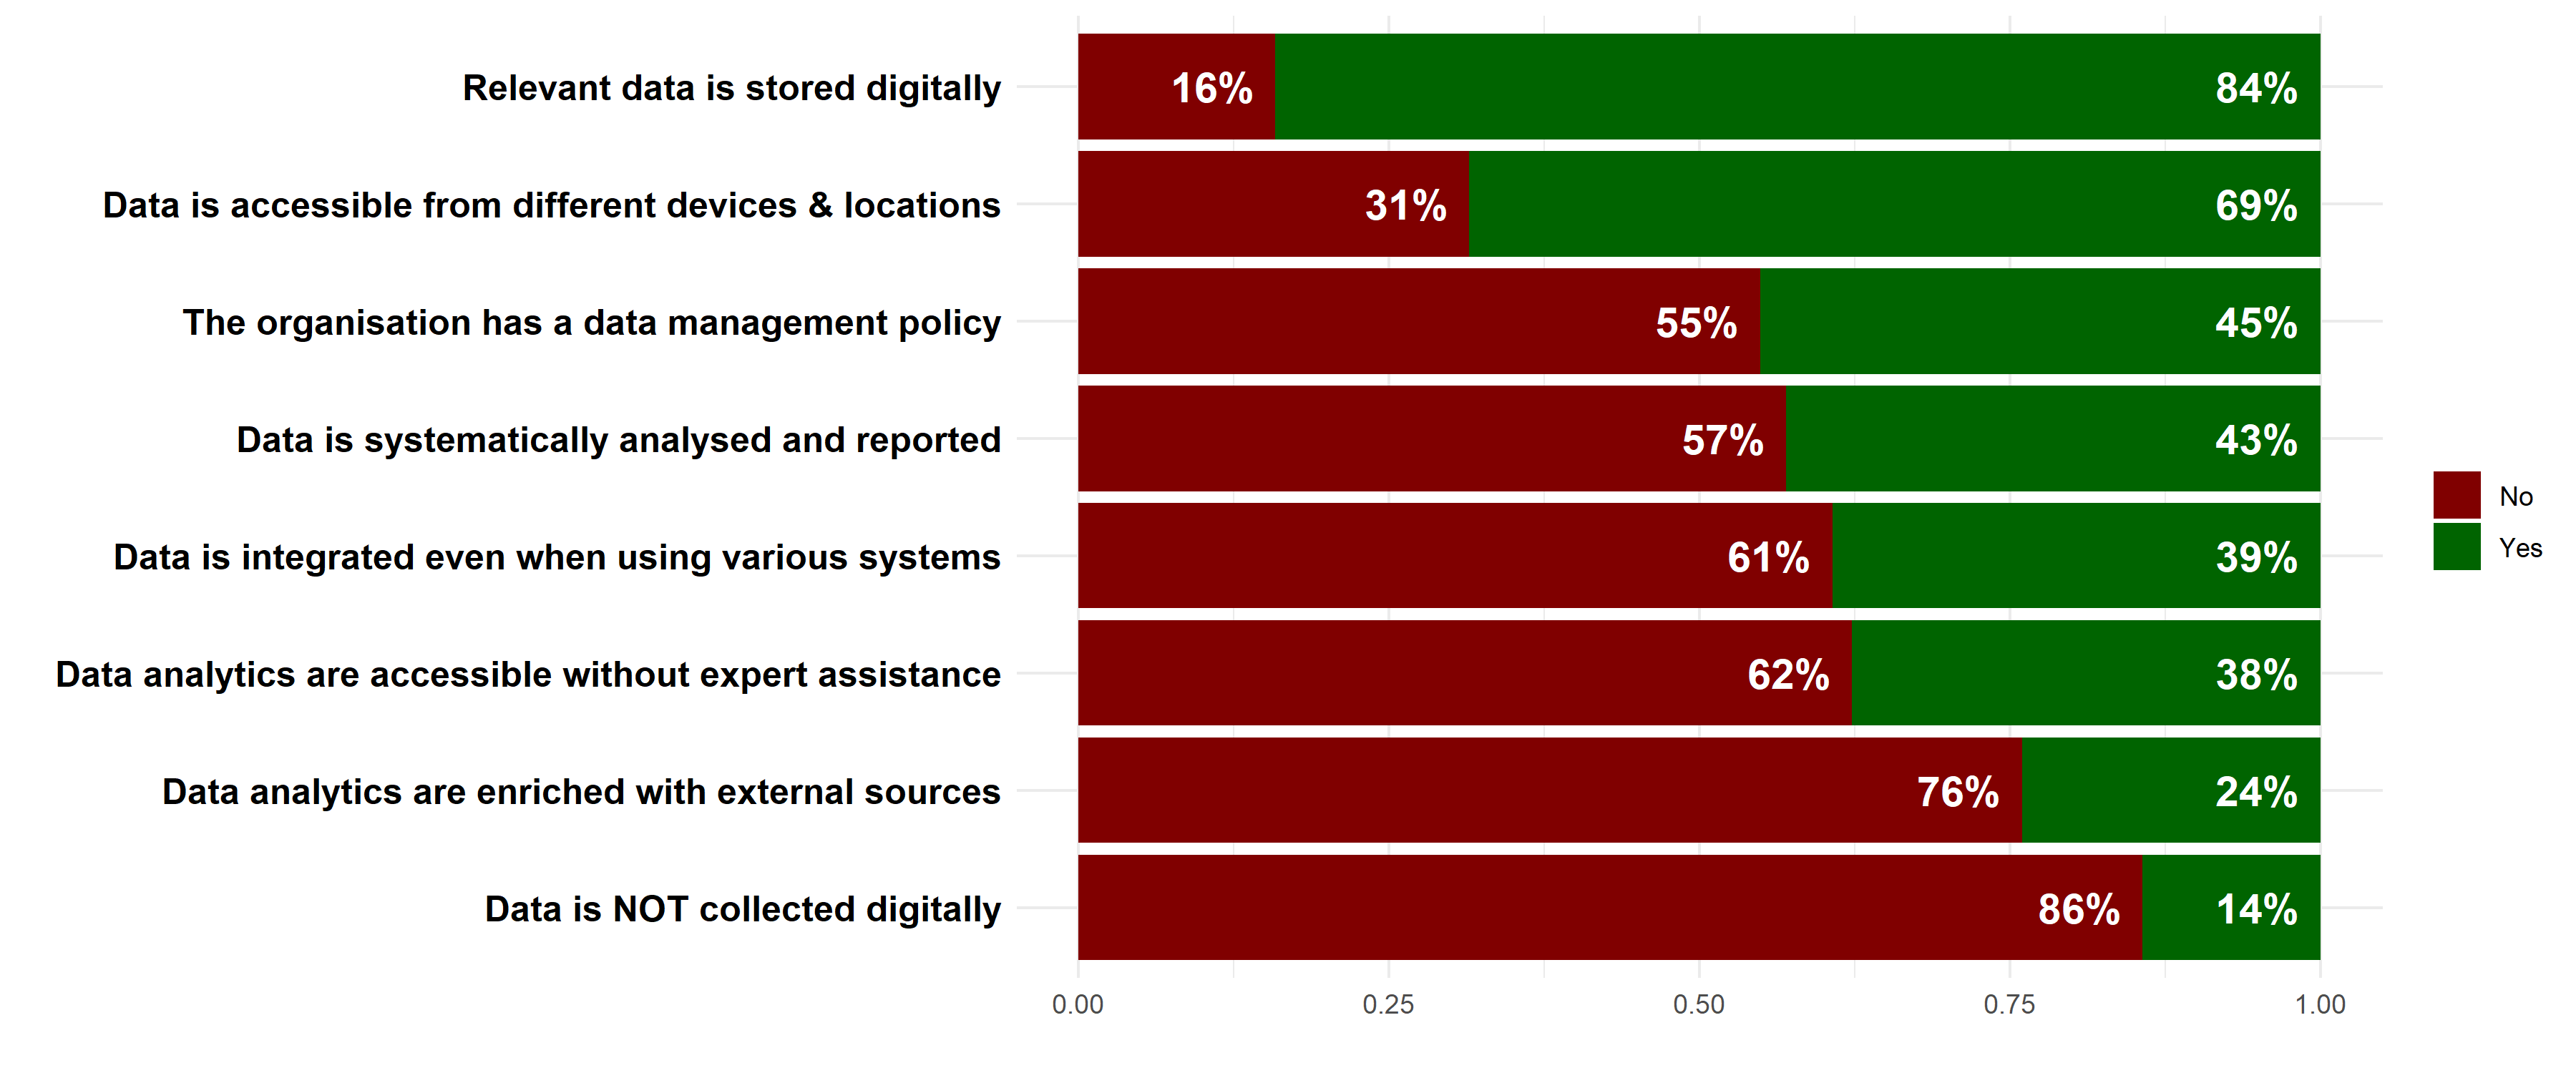
\includegraphics[width=\linewidth]{../Output/q7.png}
    \caption{\centering{Breakdown of responses to Question 7 of the DMA survey, part of the Data Management dimension.}}
    \label{fig:q7_table}
\end{figure}

\par From the responses, we can see how basic data management seems to be in place in the vast majority of firms. In fact, 84\% of respondents declare that they store digitally their data. However, this does not mean that the data is actually utilized. In fact, we can see that only 43\% of firms in the sample systematically analyze their data, and only 38\% make data analytics accessible without expert assistance (meaning they have data analytics dashboards). Even fewer firms enrich their data with external sources, making data analysis one of the most promising areas of improvement, since it appears that most firms have plenty of data, but they do not leverage it to increase their profitability. 

\par The next question in the Data Management dimension deals with cybersecurity. As we can see, this is a point of particular weakness for firms in the sample. In fact, almost a third of firms respond saying that there is not even a full backup of critical data maintained. In less than half of firms, staff is trained on cybersecurity, and only in a quarter of the firms surveyed there is a business continuity plan in case of cyber threats. Overall, these responses paint a grim picture of the state of cybersecurity for firms that replied to the DMA survey. This can be a consequence of a lack of literacy on the subject, or rather a reflection of the small size of most firms in the sample, making it infeasible for them to invest in cybersecurity measures. If the former explanation is the reason, we should expect the EDIH intervention to improve the responses to this specific question, but if the latter explanation is the real cause, it is unlikely we will see any substantial change come once $T1$ observation are available.

\begin{figure}[h!]
    \centering
    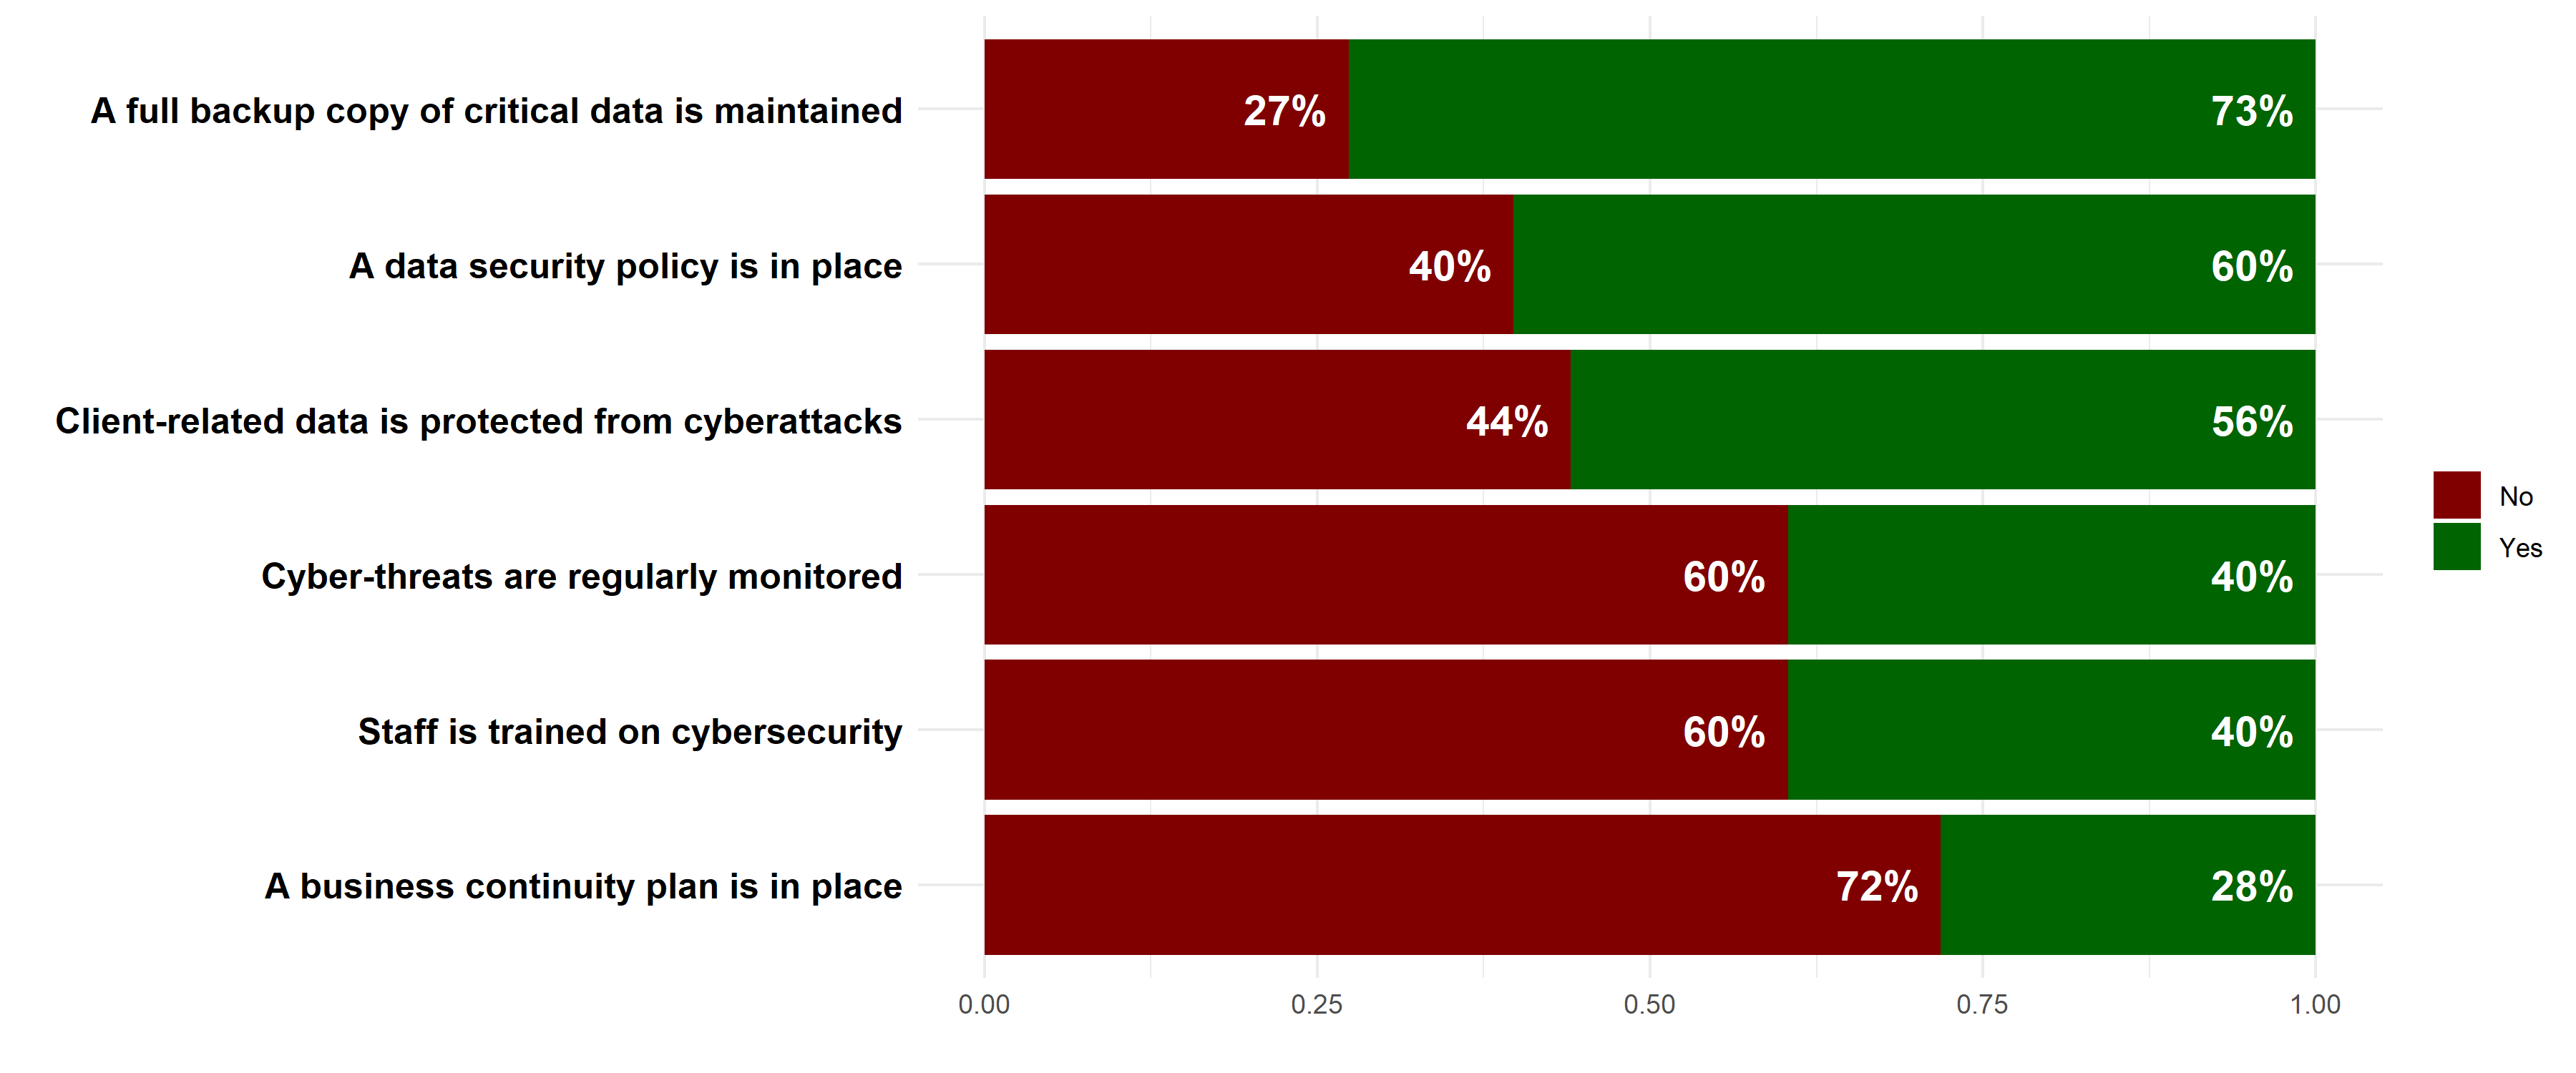
\includegraphics[width=\linewidth]{../Output/q8.png}
    \caption{\centering{Breakdown of responses to Question 8 of the DMA survey, part of the Data Management dimension.}}
    \label{fig:q8_table}
\end{figure}

\par Now let's see how the firms responded to the only question present in the dimension concerning Automation \& Intelligence. In this case, the question asked: "Which of the following technologies and business applications are your enterprise already using?". As per the question on Advanced Digital Technologies in the Digital Readiness dimension, here too there was the option to select different levels at which the implementation of the technologies was at the time of the survey's submission.




\begin{figure}[h!]
    \centering
    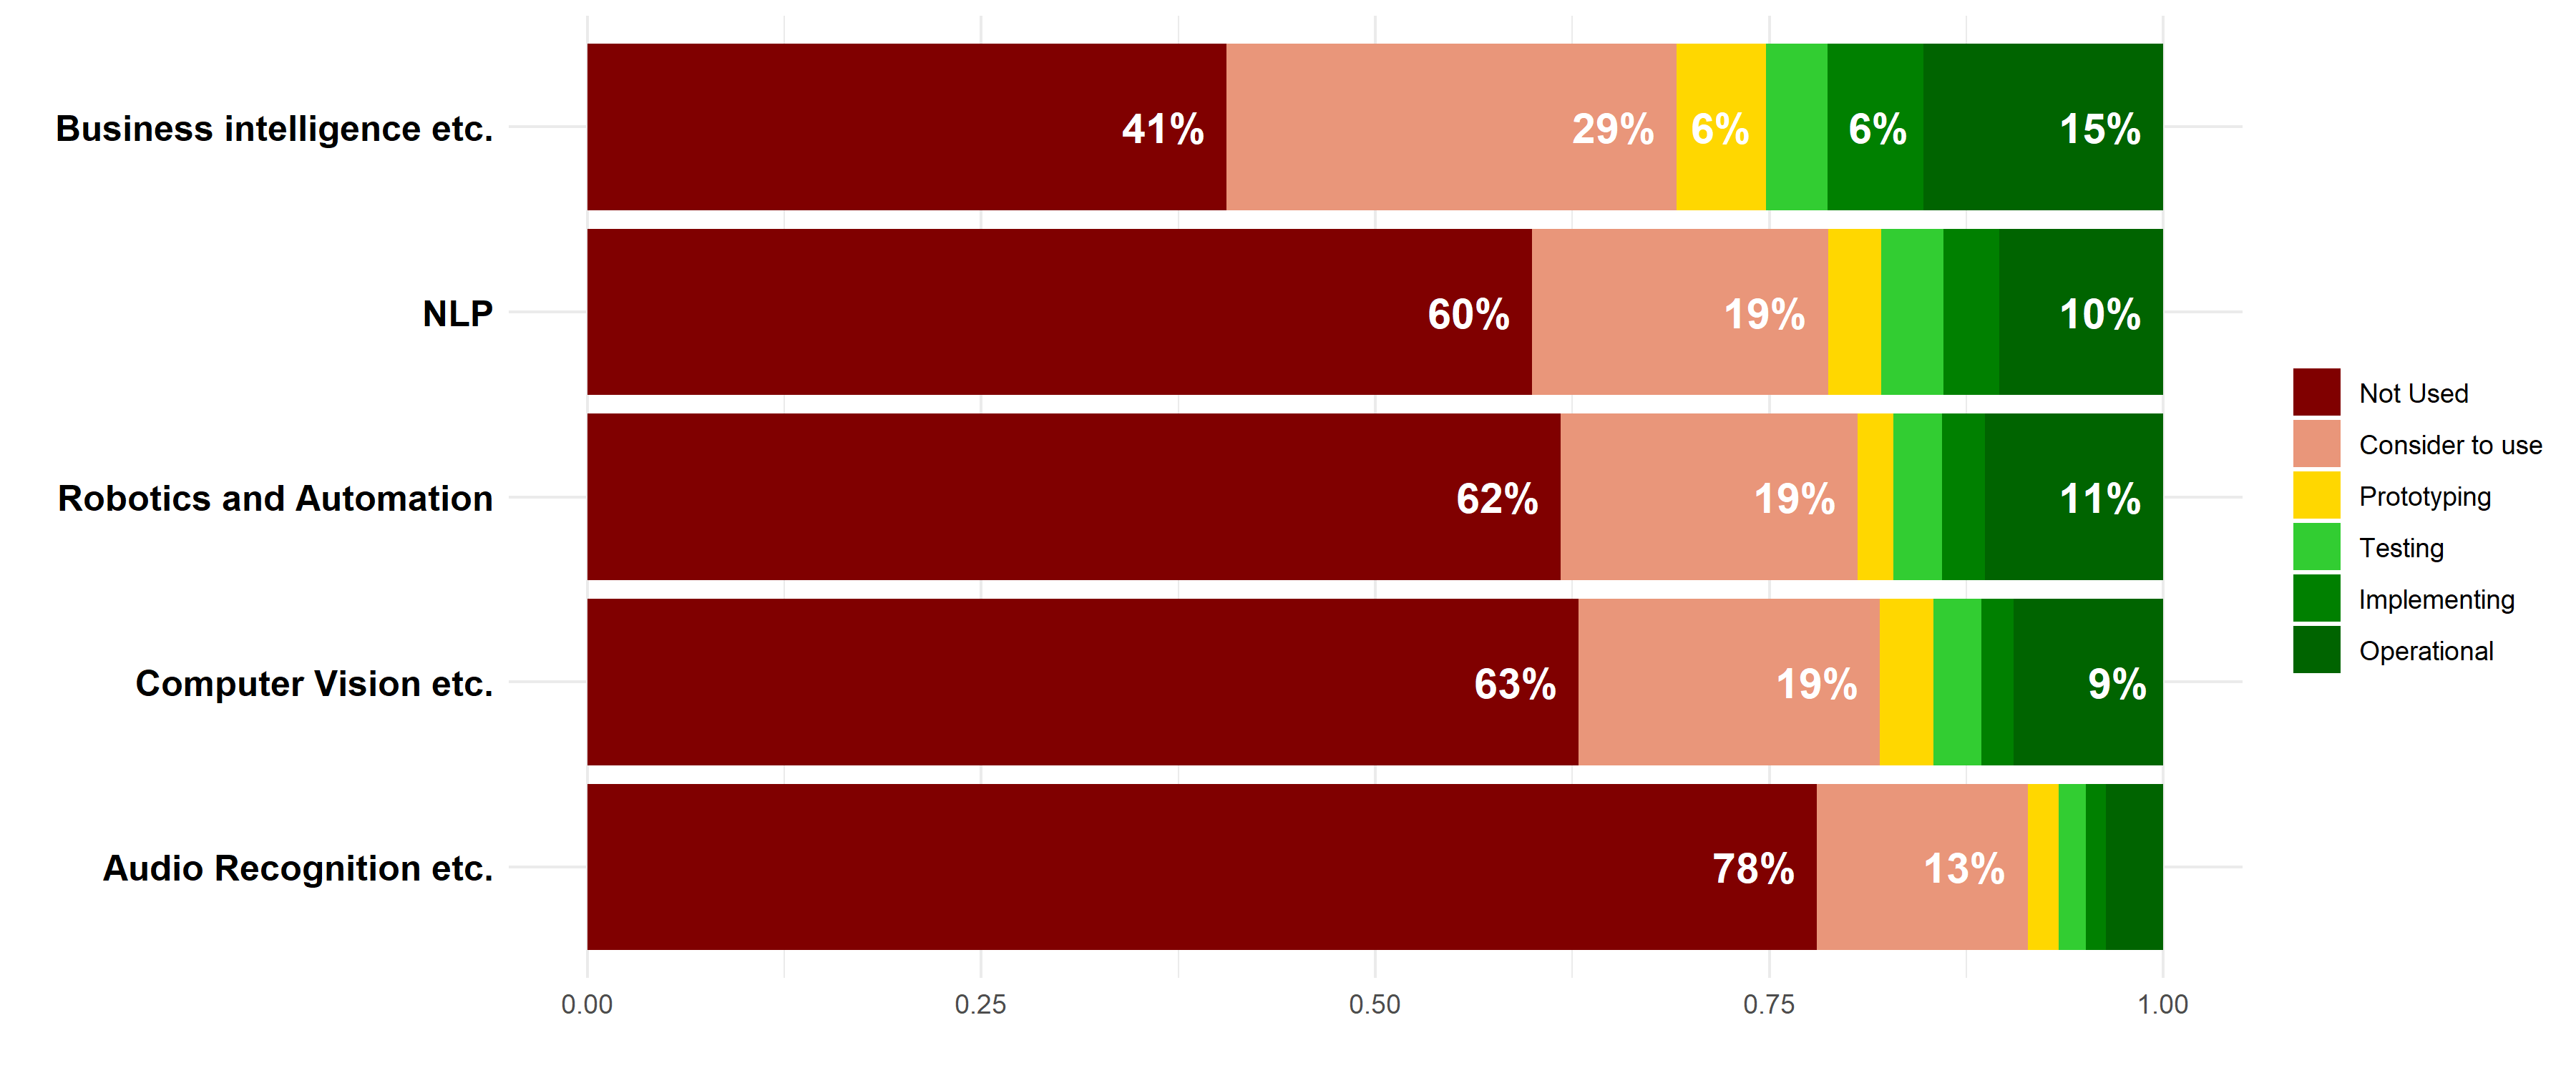
\includegraphics[width=\linewidth]{../Output/q9.png}
    \caption{\centering{Breakdown of responses to Question 9 of the DMA survey, part of the Automation \& AI dimension.}}
    \label{fig:q9_table}
\end{figure}


\par Thus, here too we can see which of these cutting-edge technologies our sample of firms finds the most interesting, by seeing which ones are considered the most, for example.

\par We can see right away that Business intelligence is by far the most sought-after technology for firms. In fact, almost 30\% of firms are considering the use of this technology. Business intelligence refers to the process of using technology to collect analyze and transform data into actionable insights for the support of decision-making. Thus, it is reasonable that firms are interested in this, and it is actually also the most widely implemented technology. 

\par Moving down, Natural Language Processing is the second-most considered technology, together with Robotics and Automation and Computer Vision, with 19\% of firms considering to implement these technologies. Audio recognition is the least implemented by far and also the least interesting to firms, perhaps also due to a smaller set of applications in some sectors, particularly manufacturing.



\par As a last section in our analysis, it is useful to look at how the different dimensions in the DMA relate to each other. This would serve as a check on the usefulness of the DMA score as a composite indicator. In fact, one general rule of thumb when dealing with composite indicators is that all dimensions should be related with one another, at least to some degree\footnote{For more details on rules and criteria for the construction of Composite Indicator Frameworks, see: \cite{oecd2008}}. The analysis of correlations between the different dimensions is going to also help us understand which ones are likely to be related, and can be helpful for future research on the subject of the DMA and the EDIH initiative more broadly.

\begin{figure}[h!]
    \centering
    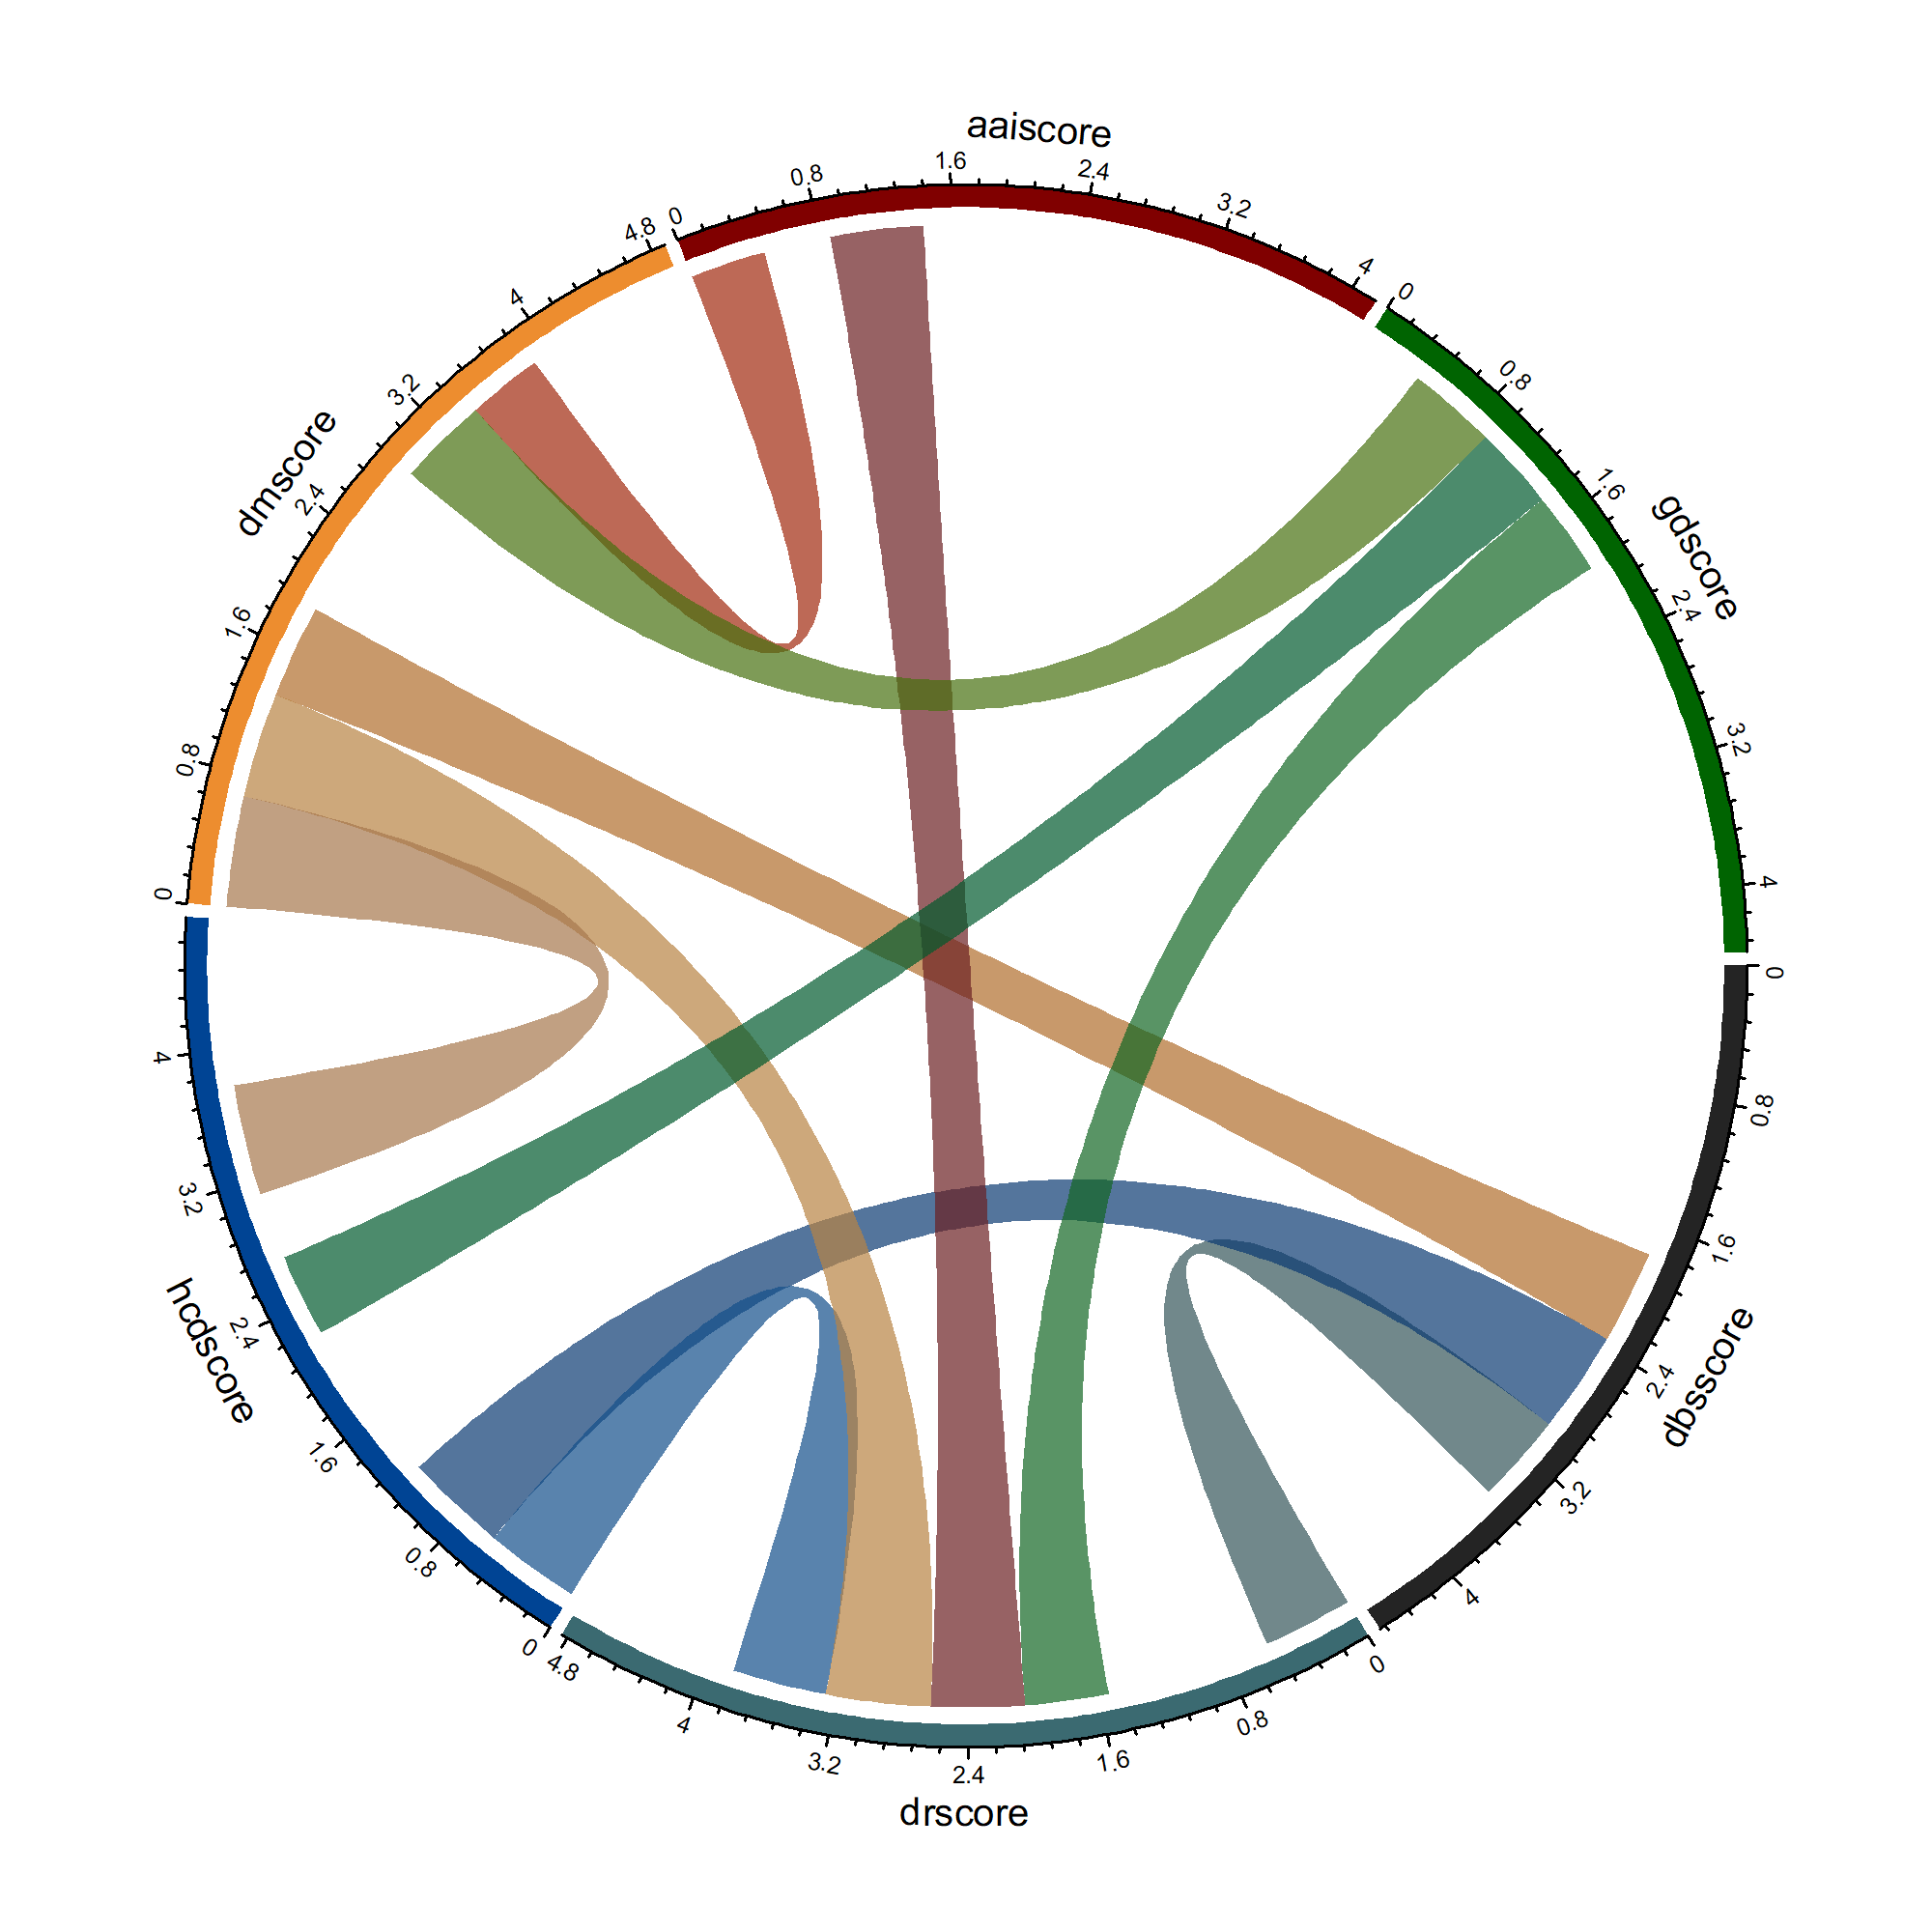
\includegraphics[width=0.65\linewidth]{../Output/theverysmallcorrmatrix_plot.png}
    \caption{\centering Circle graph of the six dimensions making up the DMA score and the correlation between them. Only correlations above 0.45 are shown in the graph; strength of the correlation is given by the thickness of the band connecting the two dimensions together. Only correlations above 0.3 are shown as lines.}
    \label{fig:circlize_graph}
\end{figure}


\par Let's start with a high level view. In this plot you can see a circular representation of the six dimension that make up the overall DMA score. From this it is immeditately apparent how some of the dimensions are more correlated with the whole compared to others. For example, digital readiness, human centric digitalization and data management are correlated with at least 0.45 correlation with most of the other dimensions in the DMA. Green digitalization and automation \& intelligence instead stand out, due to their correlations with a small subset of dimensions in the DMA.

\par As you would expect, green digitalization is most correlated with human-centric digitalization, but more interestingly also relatively strongly with data management and digital readiness. Automation \& intelligence, on the other hand, appears to be correlated only with digital readiness and data management, the only other two dimensions where uptake in digital technologies is measured directly.


\begin{figure}[h!]
    \centering
    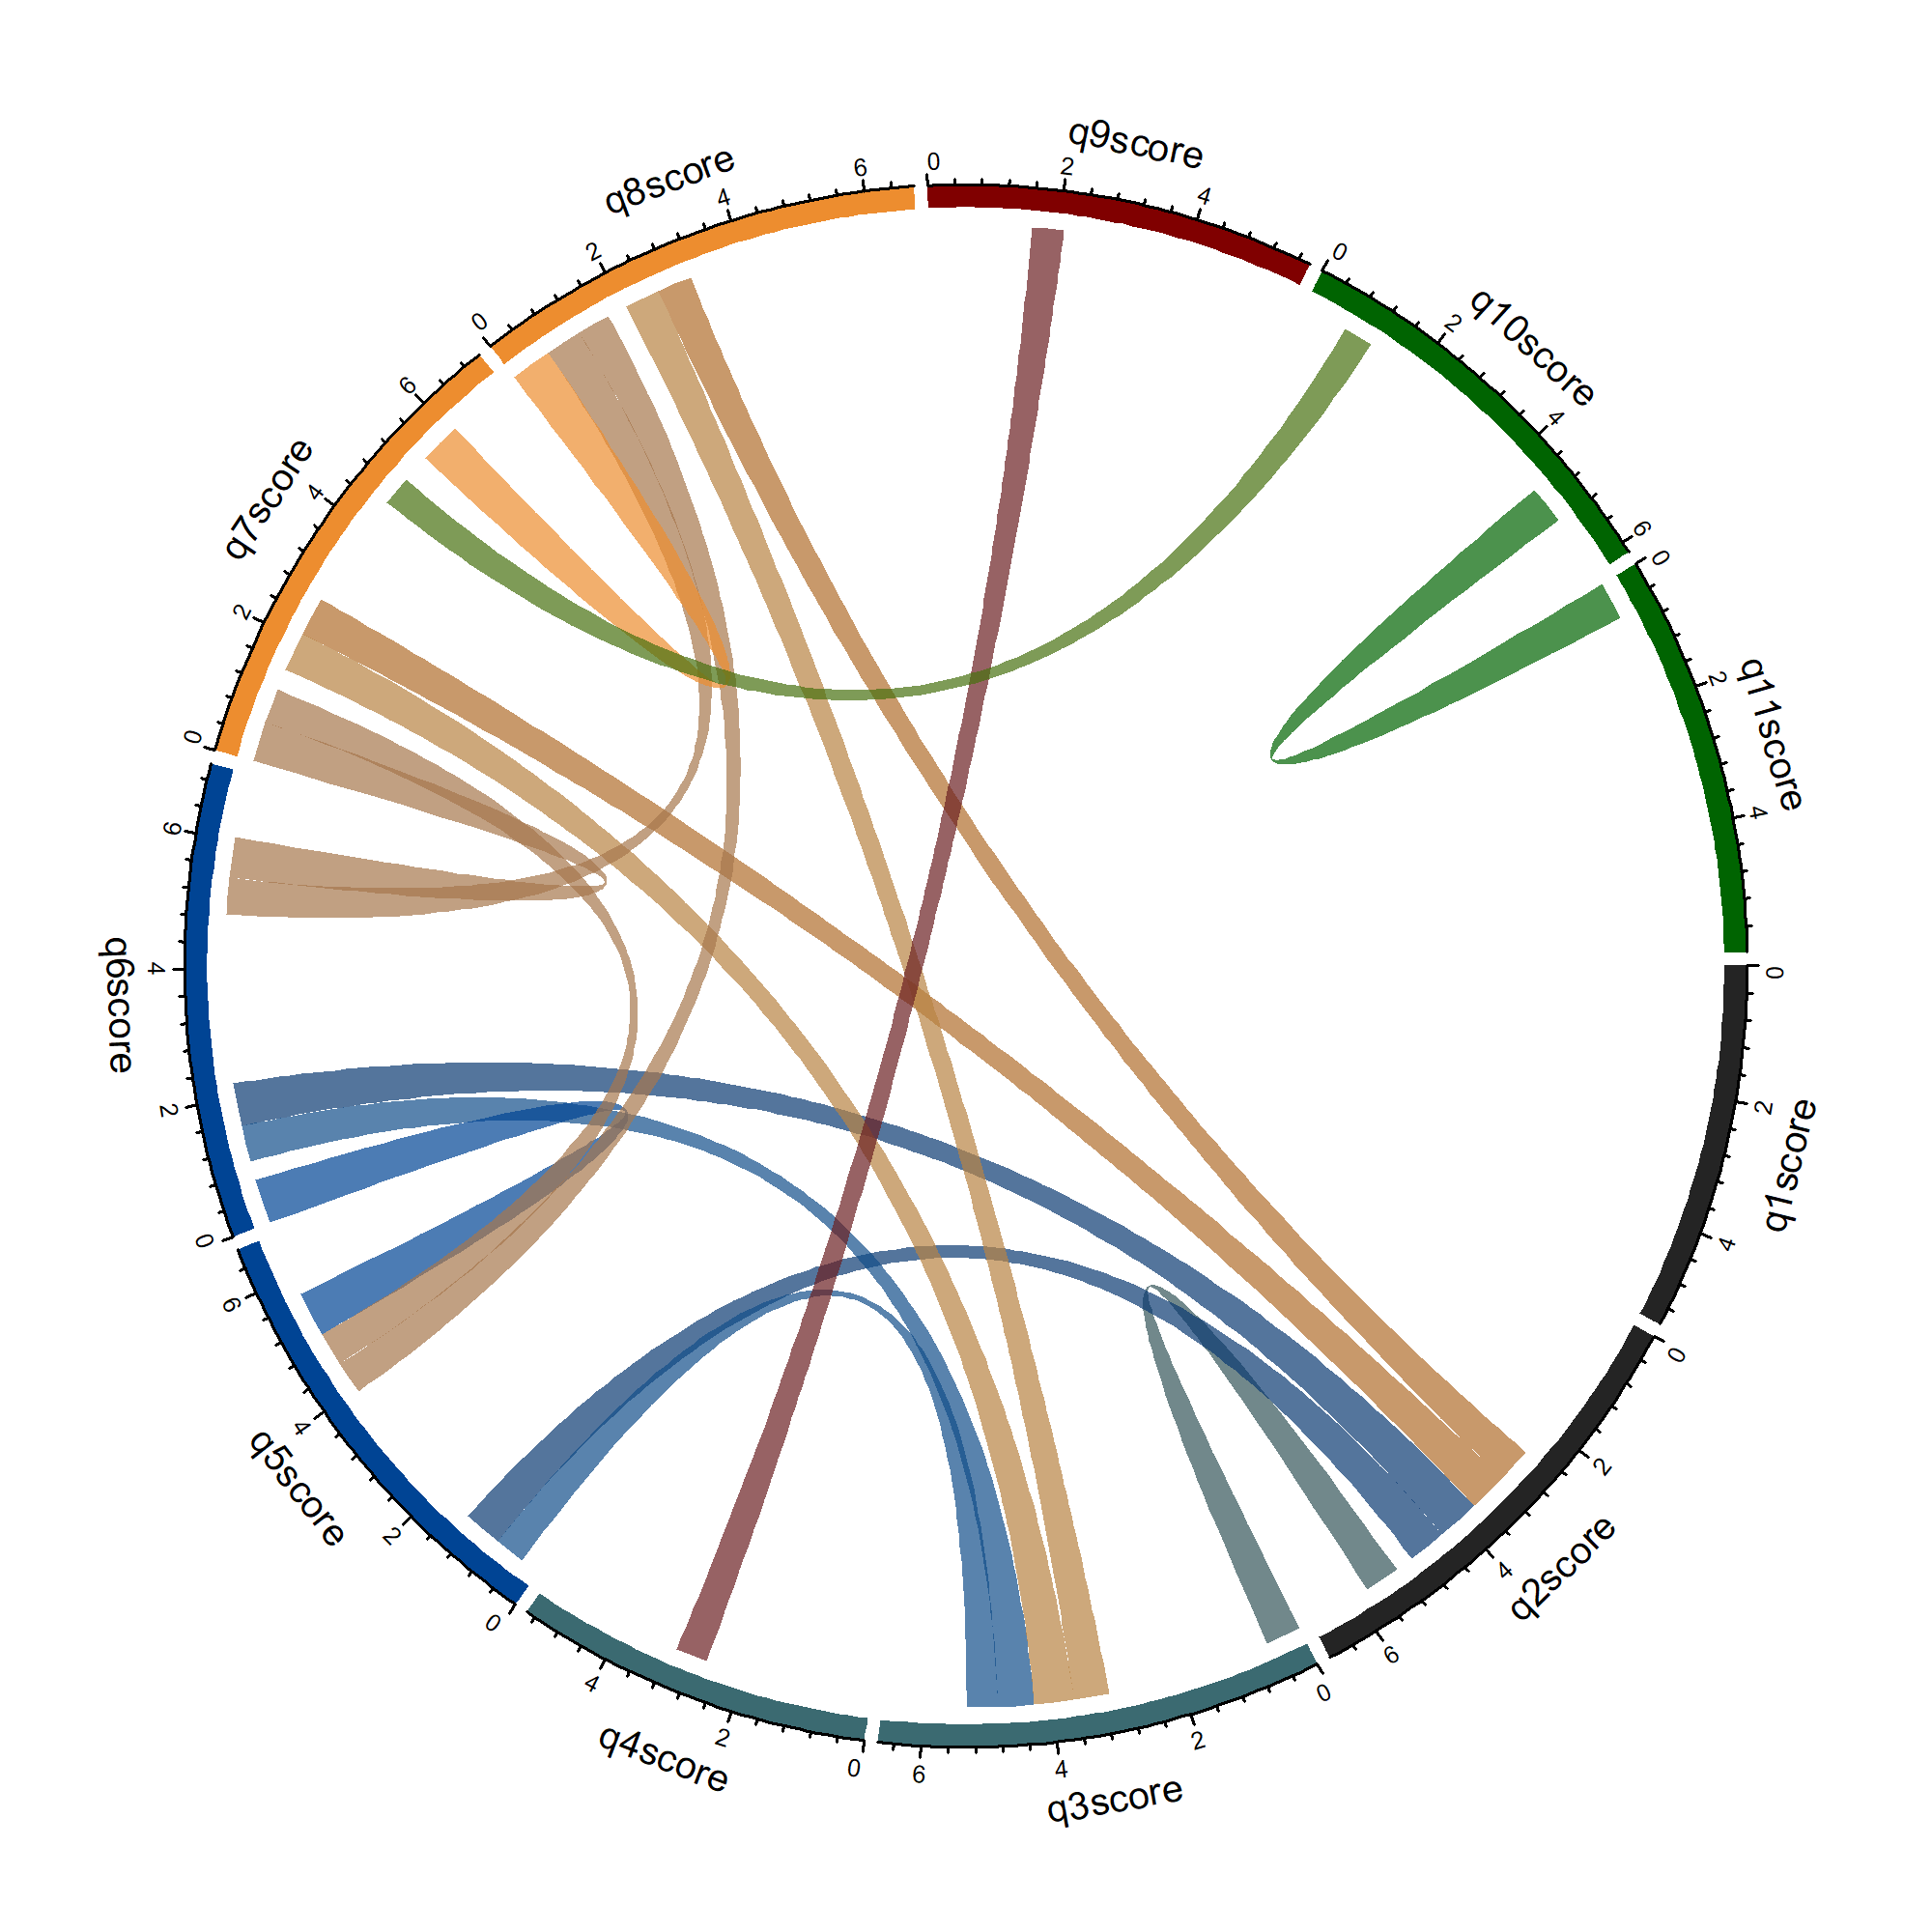
\includegraphics[width=0.65\linewidth]{../Output/thesmallcorrmatrix_plot.png}
    \caption{\centering Circle graph of all the subdimensions making up the DMA score and the correlation between them. Only correlations above 0.45 are shown in the graph; strength of the correlation is given by the thickness of the band connecting the two dimensions together.}
    \label{fig:circlize_subdimension_graph}
\end{figure}

\par We can go one level down, to look at the correlation between subdimensions, meaning individual questions in the survey. In this case, we can see how the Automation \& Intelligence dimension is actually correlated only with question 4, which deals with the uptake in Advanced Digital Technologies; furthermore, these two subdimensions are linked only between each other. This suggest that instead the Basic Digital Technologies' adoption measured in question 3 are not directly related with those technologies considered in the Advanced Digital Technologies subdimension or the Automation \& Intelligence dimension as a whole. It is also interesting to see how, when disaggregating green digitalisation into its two subdimensions, they are not linked anymore to the subdimensions making up human-centric digitalization. They are only correlated amongst themselves, and for question 10, which deals with Environmental Sustainability of business processes, with Question 7 of Data Management\footnote{This is probably due to the fact that both questions 10 and question 7 contain information on the digitized storage of data, one under the guise of paperless processes and the other while considering data management practices itself. We can see this more in detail by examining the network graph reported in the next paragraphs.}.

\par We can still zoom a little bit further down, by looking at the correlation between the individual items that make up the DMA survey. This can give us useful information on which technologies are correlated the most, and which ones instead seem to be totally unrelated with each other. To do this, I created a network graph showing each individual item in the DMA survey, for a total of 96 points in the graph.



\begin{figure}[h!]
    \centering
    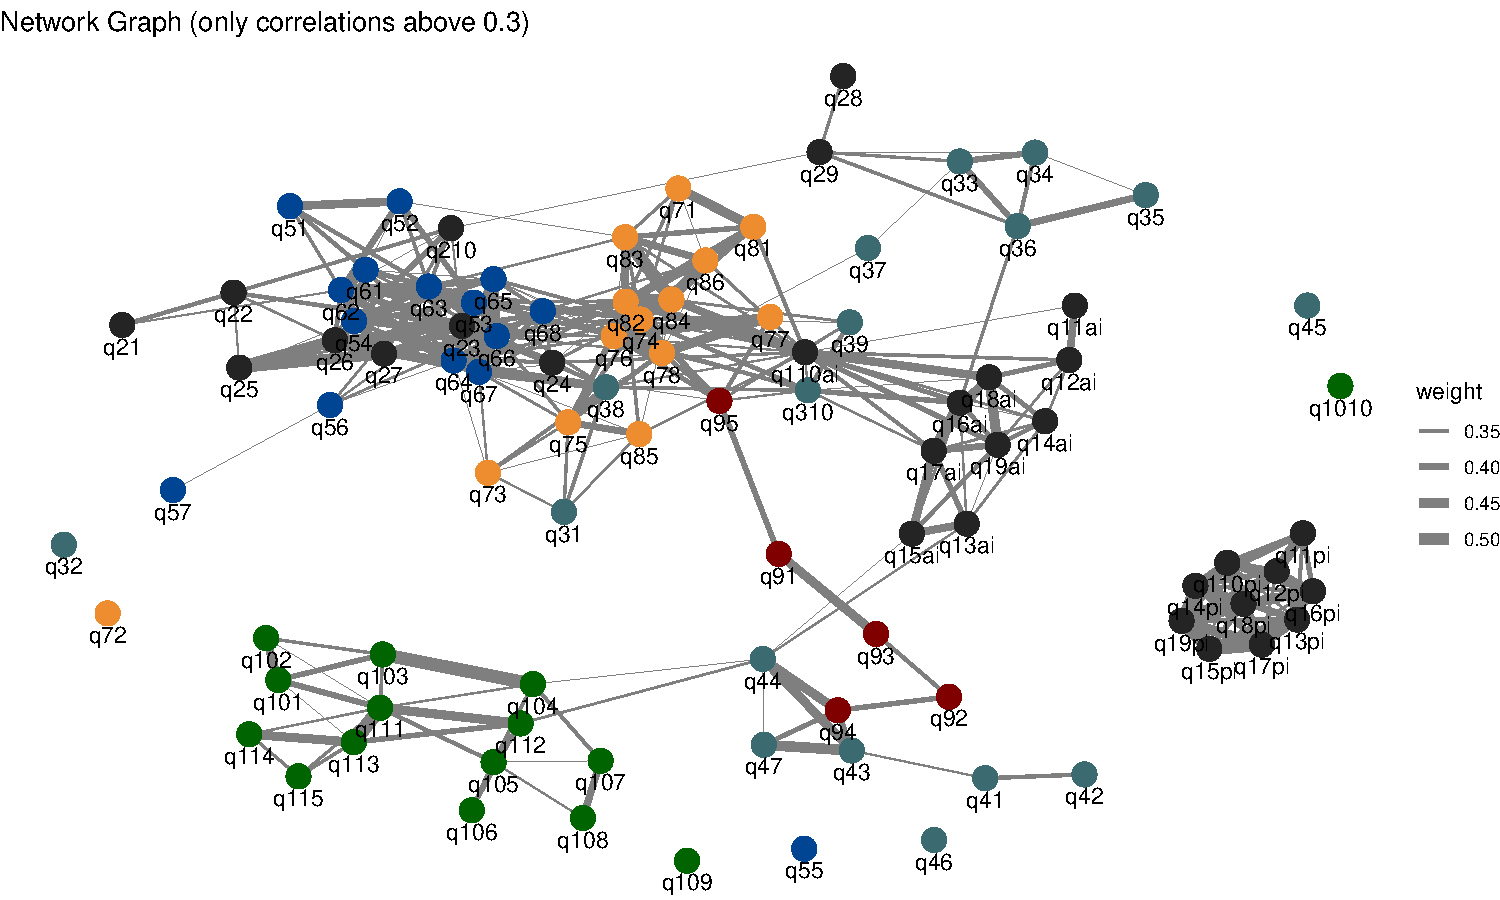
\includegraphics[width=0.8\linewidth]{../Output/network_graph.pdf}
    \caption{\centering Network graph showing the correlation between every item of the DMA. Correlation computation are performed using the \texttt{hetcor} function in R.}
    \label{fig:network_graph}
\end{figure}

\par Here we can notice most of the same patterns we identified in the circular correlation plots. For some dimensions in fact, most of the individual items are quite strongly correlated not just with each other, but also with items in other dimensions. This is the case for the human-centric digitalization and the data management dimension, as well as the second question in the digital business strategy dimension. Regarding the digital readiness dimension, and the automation \& intelligence dimension instead, there are interesting details that ought to be explored.

\par We can see right away for example that items from question 3, related to Basic Digital Technologies, are much closer to the centre of mass of our network. For example, you can see how item q38 is correlated with q67. This is because item q38 measures the adoption of a teleworking digital platform, and q67 measures if flexible working arrangements are in place in the enterprise. In this case the correlation is due to the same underlying phenomena being investigated.

\par However, if you look at the correlation between q39 and q95, the relationship seems more interesting. In fact, q39 measures through a 0-1 response if the firm has in place any kind of organizational intranet, while q95 measures the degree of adoption of business intelligence (e.g. data analytics). In this case, the technology measured is not the same, so it is interesting that at least a correlation exists\footnote{Perhaps one potential explanation is that one technology is a stepstone for the other, but until we have more information with $T1$ and eventually $T2$ observations coming from the DMA, we cannot say. Once those are available, it will be possible to see if there is a pattern in the process through which firms "unlock" new technologies}.

\par Other examples can be pointed out, such as the constellation of correlated items from question 9 and question 4, made of q94, q44, q47 and q43. These are all items measuring the adoption of technologies related to manufacturing, so it is natural that they go hand-in-hand. You can see a similar example with the q33-q34-q35-q36 agglomeration. These are all items related to digital commerce and the digital interaction with customers in a broader sense, so it is reasonable that they move together to some degree.

\par Overall, these patterns of correlations between dimensions, subdimensions, and individual items provide at least some indication that the DMA survey is working properly and as intended, allowing us to utilize it as a tool for the evaluation of the EDIH initiative in the future, as well as providing a potential basis for the analysis of the adoption pattern of individual technologies.




% \newpage

% 
% Table created by stargazer v.5.2.3 by Marek Hlavac, Social Policy Institute. E-mail: marek.hlavac at gmail.com
% Date and time: dom, gen 19, 2025 - 23:51:49
\begin{table}[!htbp] \centering 
  \caption{} 
  \label{} 
\begin{tabular}{@{\extracolsep{5pt}}lc} 
\\[-1.8ex]\hline 
\hline \\[-1.8ex] 
\\[-1.8ex] & dmascore \\ 
\hline \\[-1.8ex] 
 distance\_from\_edih & $-$0.031$^{***}$ \\ 
  & (0.009) \\ 
  & \\ 
 firm\_density & $-$0.002 \\ 
  & (0.008) \\ 
  & \\ 
 tech\_levelHigh & 8.365$^{***}$ \\ 
  & (2.860) \\ 
  & \\ 
 tech\_levelMedium & 6.308$^{**}$ \\ 
  & (2.467) \\ 
  & \\ 
 tech\_levelMedium-High & 9.160$^{***}$ \\ 
  & (1.462) \\ 
  & \\ 
 tech\_levelMedium-Low & 5.758$^{***}$ \\ 
  & (1.403) \\ 
  & \\ 
 operating\_revenue\_turnover & 0.033$^{***}$ \\ 
  & (0.007) \\ 
  & \\ 
 employees & 3.059$^{**}$ \\ 
  & (1.448) \\ 
  & \\ 
 liquidity\_ratio & 0.112 \\ 
  & (0.192) \\ 
  & \\ 
 solvency\_ratio\_assetbased & $-$0.025 \\ 
  & (0.021) \\ 
  & \\ 
\hline \\[-1.8ex] 
Observations & 1,221 \\ 
R$^{2}$ & 0.115 \\ 
Adjusted R$^{2}$ & 0.102 \\ 
Residual Std. Error & 16.177 (df = 1202) \\ 
F Statistic & 8.690$^{***}$ (df = 18; 1202) \\ 
\hline 
\hline \\[-1.8ex] 
\textit{Note:}  & \multicolumn{1}{r}{$^{*}$p$<$0.1; $^{**}$p$<$0.05; $^{***}$p$<$0.01} \\ 
\end{tabular} 
\end{table} 










\newpage
\chapter{What are the drivers of participation?}
\par As we have already discussed, the current state of the EDIH initiative doesn't allow for the analysis of the impact of the policy on firms' digital maturity. The reason leads back to the fact that the program itself is too recent (EDIH activities began in spring of 2023), thus we have no way of knowing what its impact has been, based on firm's financials or even based just on scores from future submissions of the DMA survey\footnote{As of now, we have only a limited number of observations related to T1 issuings of the DMA survey, taken 1 year after the intervention of the EDIH. This initial data indicates a betterment of the Digital Maturity Score, at least in treated firms, even for those sections related to the adoption of specific advanced technologies. However, since the DMA was never submitted to a control group of firms not participating in the program, an analysis of this type would not be able to establish causality.}.

\par However, what we can do is investigate what are the driving factors that are leading firms to participate in the program itself. This can lead us to better understand if the targeting of the policy is working properly, or for example if there are some steps that can be taken in order to increase participation in the program itself. Furthermore, understanding the drivers of participation can also give us insights into the size and sign of the potential bias that can be present in the future analysis of the impact of the program on firms' digital maturity\footnote{For instance, if the analysis were to suggest that one of the positive drivers of participation is firm size, we can hypothesize that when measuring the impact of the policy only on the treated firms, the bias on the effect of digital maturity will be positive, since we can reasonably assume that larger firms can benefit more easily from digitalization initiatives. Conversely, if smaller firms are more likely to participate, the bias might be negative.}.

\par To perform the analysis, I have matched the firms that participated in the EDIH initiative with the ORBIS database to retrieve firm-level financial information (such as their size, country, sector in which they operate, and indicators of financial performance).

\par Once having had the data on treated firms, I have constructed a synthetic control group of untreated firms. These control firms will be selected randomly from the ORBIS database. After constructing the control group, first of all I've compared the treated and control firms to identify any significant differences in their characteristics. This comparison is instrumental to understand the factors that may influence a firm's decision to participate in the EDIH initiative.

\par As an additional information to add on top of country information on where the firms are located, I decided to assess the effect of the distance of firms from the closest EDIH hub. The working hypothesis is that firms that are sited closer to an EDIH hub are more likely to have heard about the program and thus to participate in it. Knowing how distance affects firms' participation can be instrumental in understanding if an expansion in the number of hubs or in their geographical coverage can lead to an increase in participation. Also, to account for the possibility of the effect being confused by areas with a large concentration of firms (which are more likely to have an EDIH hub nearby, and thus more likely to participate), I have computed a measure of firm density. To compute both density and distance, I geocoded the firms' addresses, taken from the ORBIS database or from the DMA survey itself.

\par Finally, I have run a probit regression model to analyze the drivers of participation in the EDIH initiative. The regression model includes various firm-level characteristics as independent variables, and the dependent variable is a dummy variable indicating whether the firm participated in the EDIH initiative.

\par In the following sections, I am going to describe the matching process, the construction of the control group, the treated-control comparison, the geocoding process, and the results of the regression analysis in detail, as well as some robustness checks on those results.

\newpage
\section{Matching of treated firms with ORBIS}

\par To safely match the treated firms with the ORBIS database, I have used the data from the DMA survey replies. Every firm, when submitting the DMA to the Digital Transformation Accelerator platform, has to provide basic company information. Among other things, the database includes firms' legal names, as well as VAT numbers. 

\par These information can be used to match companies with data in ORBIS. However, the DMA tool does not automatically check for invalid VAT numbers, thus some of the reported VAT codes are incorrect. Furthermore, I was relying on WRDS as the website to download the ORBIS database, and WRDS allows for downloading big chunks of data, such as all firms in Europe (or filtering by country, in each European Member State), but only for some specific variables. Among the variables that can be downloaded, there is no VAT code. Thus, I had to rely on company names to match the firms. This is not ideal, since it is possible to have misspellings or different ways of writing the same company name.

\par Thus, to match the treated firms i proceeded in the following way:

\begin{enumerate}
    \item I downloaded the whole universe of firms in ORBIS country by country (for 18 EU Member States where the number of firms participating in the EDIH initiative was the highest), saving them as \texttt{Orbis-COUNTRYCODE-Universe.csv} files.
    \item To have a more efficient code, I loaded the files into memory one country at a time and then, for every country in my DMA database, I computed the Jaro-Winkler distance\footnote{The Jaro-Winkler distance is defined as being equal to 1 minus the Jaro-Winkler similarity: $$dist(JW) = 1 - sim(JW)$$} between that firm's name and that of every company in that country's ORBIS universe, substituting the match every time a smaller distance was found until a threshold of 0.01 was reached\footnote{The threshold of 0.01 was chosen after some trial and error, to minimize the number of false positives while still speeding up the matching process.}. After having done this for every country's ORBIS universe, I saved the results in a .csv file, containing the matched DMA company name, the ORBIS company name, and the corresponding BvD ID number as well as the VAT code from the DMA database.
    \item This allowed me to then download the financial data for the matched firms by searching them in ORBIS through the BvD ID number. I then checked if the VAT code corresponded to the one in the DMA database, by again computing the Jaro-Winkler distance between the 2 strings.\footnote{This was done to make sure that simple misspellings in the input of the VAT code would not cause the matching to be negative.} If the distance was above the threshold, I inspected other variables to check if the match was correct and the VAT code was indeed incorrectly specified.
\end{enumerate}

\par As I was mentioning in the previous chapter on the DMA survey, at the time the analysis was performed the firms in the database were 3204, out of which I was able to match through this procedure 2886 of them. Thus, the percentage of matched firms through this procedure was roughly 90\%. The remaining 10\% of firms were not matched for a number of potential reasons, that can have different implications on the analysis I am going to perform. Potential reasons include:
\begin{itemize}
    \item The firm was not present in the ORBIS database, either due to the firm being too small, too young, or perhaps being located in a country were ORBIS coverage is not perfect.
    \item The firm was present in the ORBIS database, but the name was misspelled or written in a different way, and the Jaro-Winkler distance was too high to match the firm, and instead it matched to a completely different one. This can be the case in particular for firms with shorter names, or sometimes cited with their acronyms.
\end{itemize}
\par I will discuss this more once I present the design of the control group, but for now it is important to note that if the second case is the one driving the majority of the non-matches, since having shorter names or acronyms is not likely to be significantly correlated with any other firm-level characteristics, the bias introduced by the non-matches is likely to be small and negligible.
\par However, if the non-matched firms are mostly belonging to the first case, then we have to keep in mind that it is possible that the matched firms are systematically larger in size, possibly older, and located in country with better ORBIS coverage with respect to the overall sample of firms that participated to the EDIH initiative.


\section{Creating the Control Group}

\par When designing the control group, one has to consider the aim of the analysis it is going to be performed with it. 
\par For example, if the aim is to estimate the impact of the EDIH initiative on firms' digital maturity, the control group should be constructed in a way that it is as similar as possible to the treated group, except for the fact that it did not participate in the program. This is because the aim of the analysis is to estimate the counterfactual: what would have happened to the treated firms if they had not participated in the program. 
\par The case of my analysis however, is a bit different. Since we are trying to estimate the drivers of participation in the program, the control group should be as "agnostic" as possible, the reason being that the best control group for our analysis would be the one that is most representative of the population of firms that could have participated in the program (so, in theory, the whole population of firms in the EU). 
\par Since I cannot have access to the whole population of firms, but only to a subset of them who are reported in the ORBIS database, the best control group is the one that is most representative of the population of firms that are in the ORBIS database. This choice of course has implications, since ORBIS coverage is not the same across all countries, and it is not independent of firm-level characteristics.
\par However, since the treated firms included in the analysis are also only the ones that are present in ORBIS, the bias introduced is likely to be attenuated, since they will share the same selection bias.
\par It should also be noted that if the characteristics leading to better coverage in ORBIS are also the ones leading to participation in the EDIH initiative, the bias introduced by the control group can be positive. 

\par All this taken into account, I have constructed the control group in the following way: I have taken all the firms in the ORBIS database for the 18 selected countries, and picked random BvD IDs with the only constraint that the proportion of firms from a specific country in the synthetic control group should be the same as the proportion of firms from that country in the overall ORBIS database. This was done to ensure that the control group is representative of the population of firms in the ORBIS database.\footnote{Representativeness with respect to other firm-level characteristics was not considered as a constraint. However, the large number of the sampled firms making up the control group should allow for representativeness due to the law of large numbers.}
\par After running this procedure, I had a list of 100000 firms, for which I then downloaded firm-level characteristics from the ORBIS database.
\par After doing this, everything was ready to proceed with the initial comparison between treated and controls.

\section{Treated - Control Comparison}

\par In the table below, I present the results of an initial comparison between treated and control firms. The table shows the mean and median values of the main firm-level characteristics for the two groups, as well as the results of a t-test for the equality of means between the two groups. The t-test is performed for each variable, and the p-value is reported in the last column.

% latex table generated in R 4.4.2 by xtable 1.8-4 package
% Wed Apr  9 18:31:31 2025
\begin{table}[ht]
\centering
\begin{tabular}{lrrr}
  \hline
Statistic & Treated\_0 & Treated\_1 & p\_value \\ 
  \hline
N & 3643.00 & 1249.00 &  \\ 
  Mean\_Employees & 0.03 & 0.09 & 0.00 \\ 
  SD\_Employees & 0.17 & 0.37 &  \\ 
  Mean\_TotalAssets & 14.09 & 15.18 & 0.80 \\ 
  SD\_TotalAssets & 185.97 & 108.15 &  \\ 
  Mean\_LiquidityRatio & 4.15 & 2.33 & 0.00 \\ 
  SD\_LiquidityRatio & 8.41 & 2.90 &  \\ 
  Mean\_Solvency & 37.65 & 50.51 & 0.00 \\ 
  SD\_Solvency & 35.45 & 25.62 &  \\ 
  Mean\_turnover & 9.15 & 16.02 & 0.00 \\ 
  SD\_turnover & 70.39 & 74.00 &  \\ 
   \hline
\end{tabular}
\caption{Comparison between Control Firms (Treated = 0) and Treated ones (Treated = 1), with p-values for the t-test of equal means} 
\end{table}



\par What is immediately noticeable from the first line, where the number of observations for each group is reported, is that both groups shrank in number. This is because not all firms in the ORBIS database have complete financial information, and thus some of them were dropped from the analysis. 
\par To limit this issue, I restricted the analysis to variables that had at most 25\% of \texttt{NAs} observations in each of the two datasets. However, since the observations were retained for the analysis only if all variables had \texttt{non-NA} values, the drop in observations was still significant. The number of treated firms dropped from 2886 to 1249, while the number of control firms dropped from 100000 to 3643 firms\footnote{It should be noted here that the very high sample size for the control group was chosen specifically to make sure that after the drop in observations, the size of the database was still considerably large}.

\par Moving on to the initial comparison of means in the 2 groups, we can see how for the variables showed in the table the means are significantly different. This is confirmed by the t-test, which reports a p-value of 0 for all variables except for total assets, where the p-value is 0.80, probably to the relatively high standard deviation making it difficult to detect a significant difference in means.
\par The comparison highlights something that could be already expected: the firms participating in the EDIH initiative differ significantly from the overall population of firms in ORBIS. However, the sign is what is most interesting: treated firms seem to be having more employees, a better value of the liquidity ratio, higher solvency ratios and turnover (while for total assets the difference from the simple t-test is not significant).

\par We can investigate a little bit further by comparing the distributions of the variables in the treated and control group, variable by variable. this is done in the following figures. There you can see how the treated firms' frequency distribution (in blue) compares to the control group (in red), as well as a kernel density function estimating the distribution of the variable based on the data. In every graph, above you can also see reported the p-value of the KS-test, which tests the null hypothesis that the two distributions are the same. Since the KS-test is a non-parametric test, it allows us to confirm that also in the case of total assets, the two distributions are significantly different.


\begin{figure}[ht]
    \centering
    \begin{subfigure}[b]{0.45\textwidth}
        \centering
        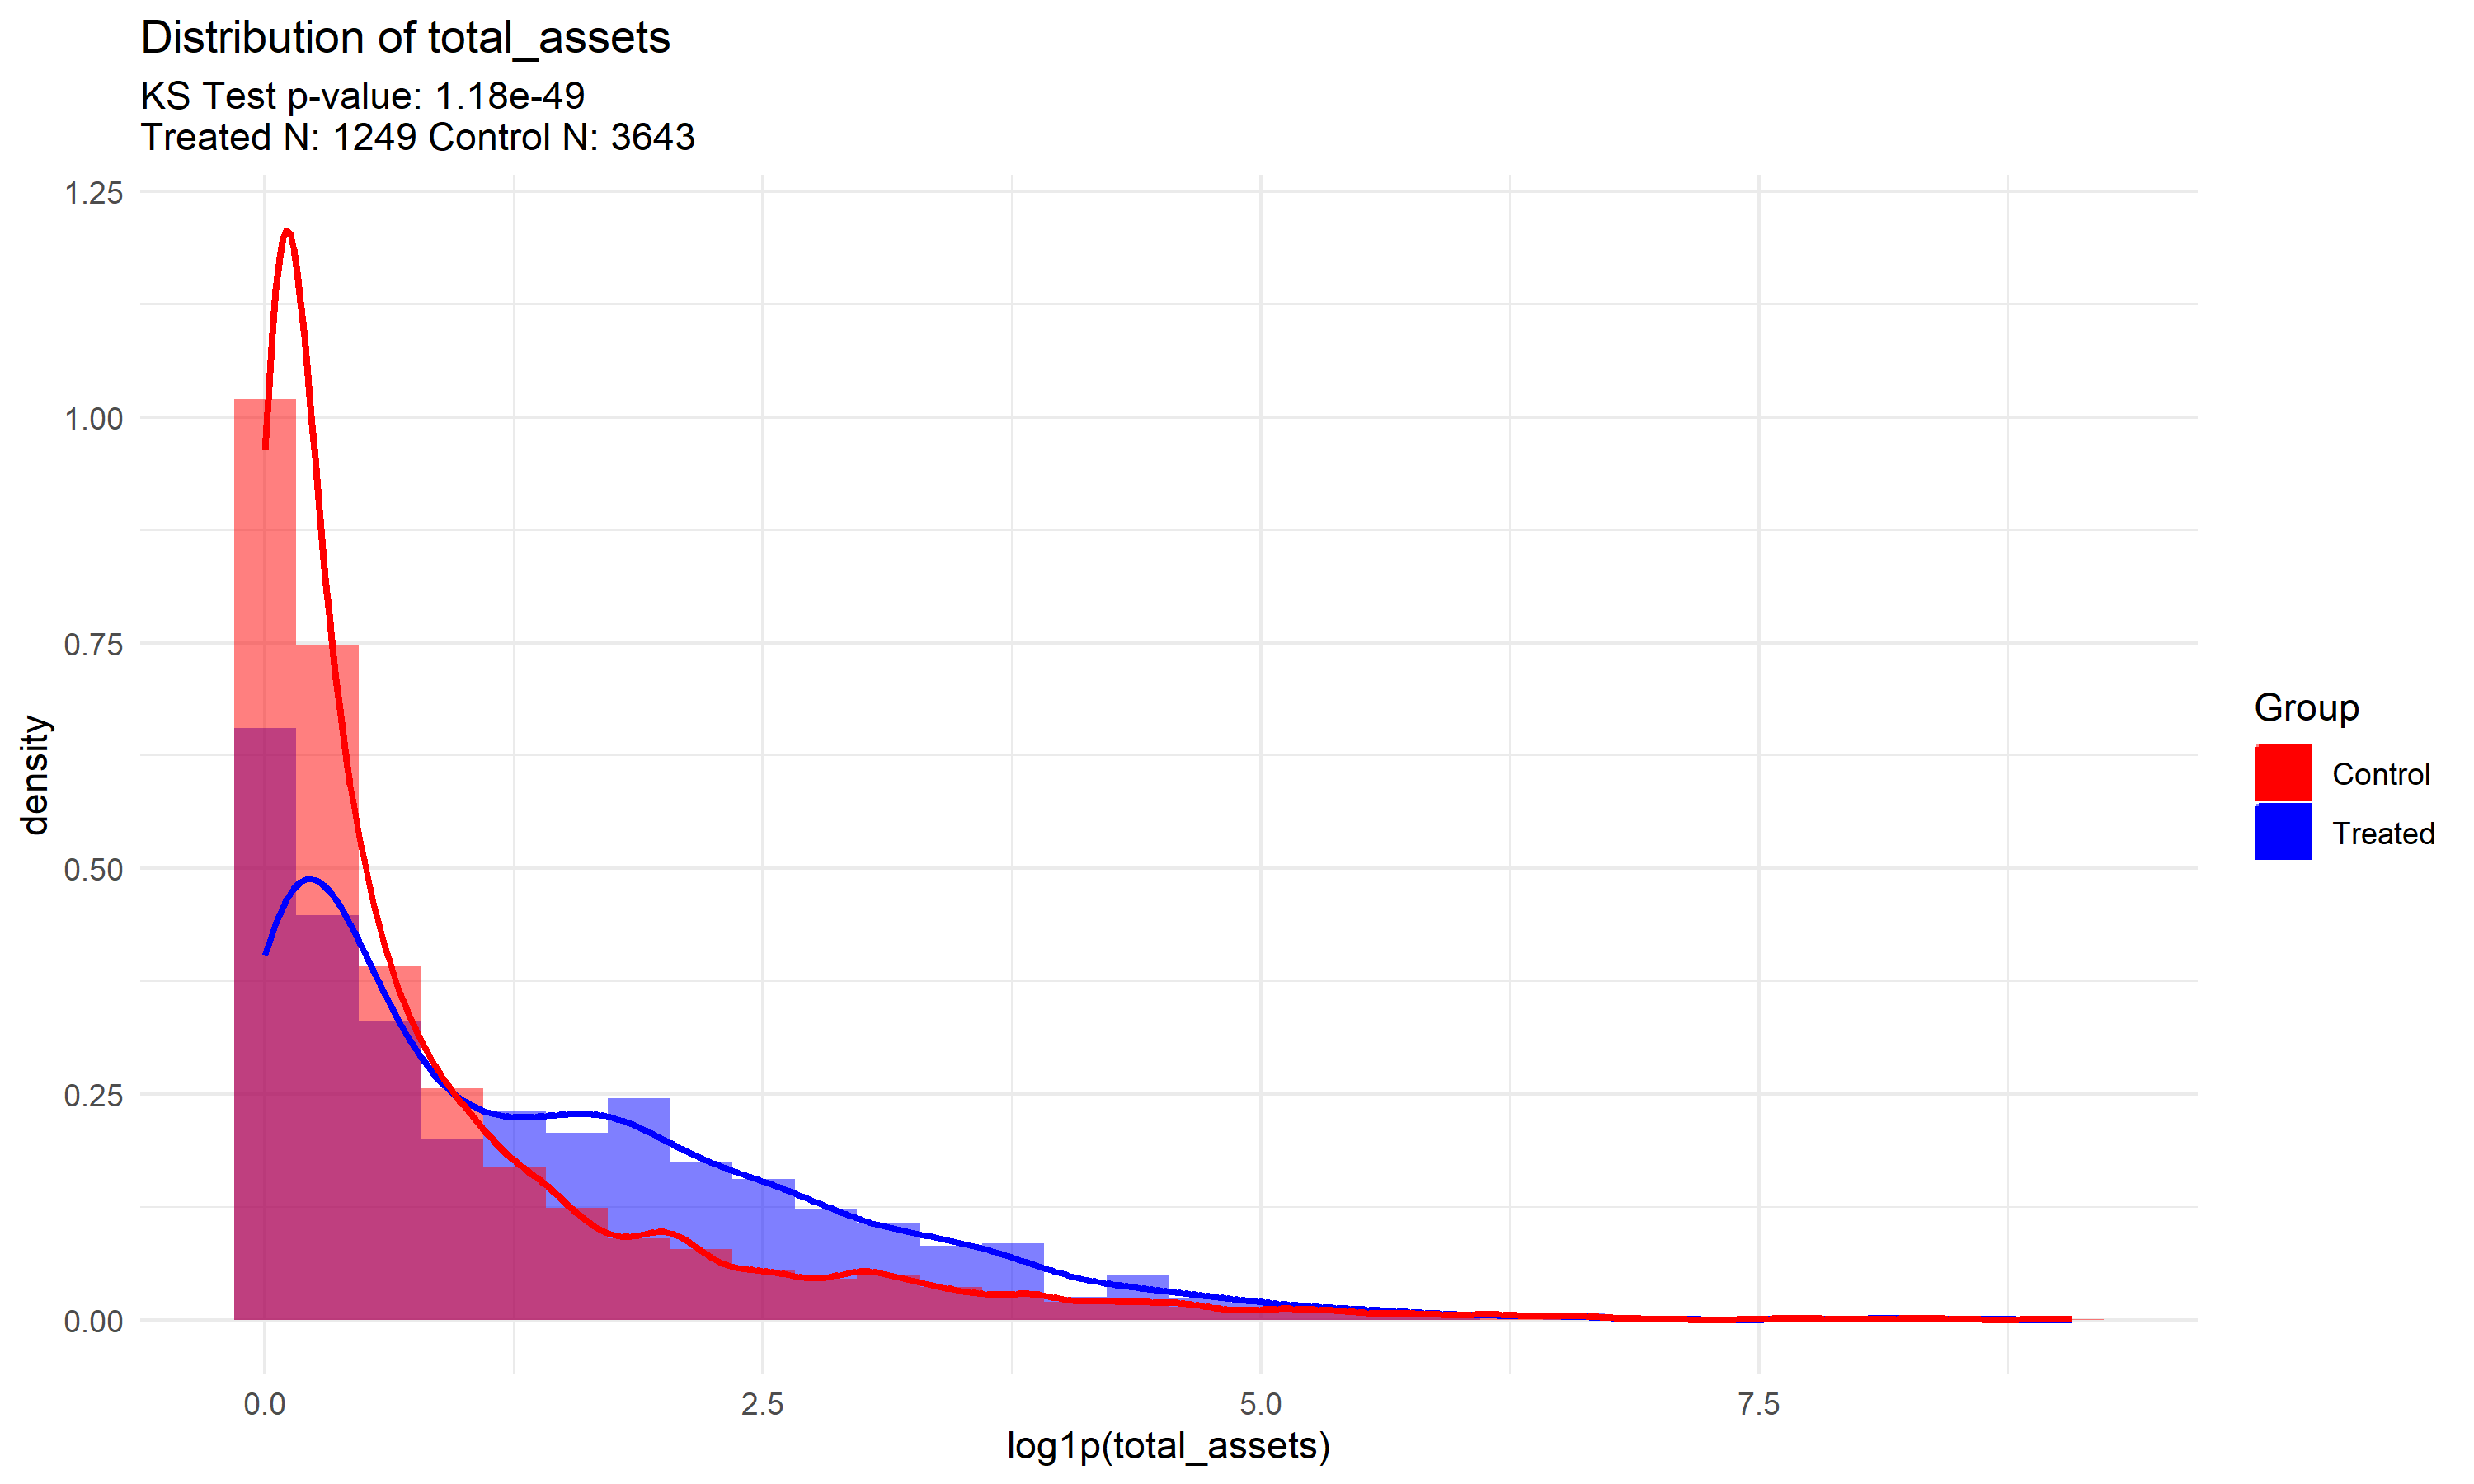
\includegraphics[width=\linewidth]{../Output/distrib_compare_total_assets_allcountries.png}
        \caption{Total Assets}
        \label{fig:total_assets}
    \end{subfigure}
    \hfill
    \begin{subfigure}[b]{0.45\textwidth}
        \centering
        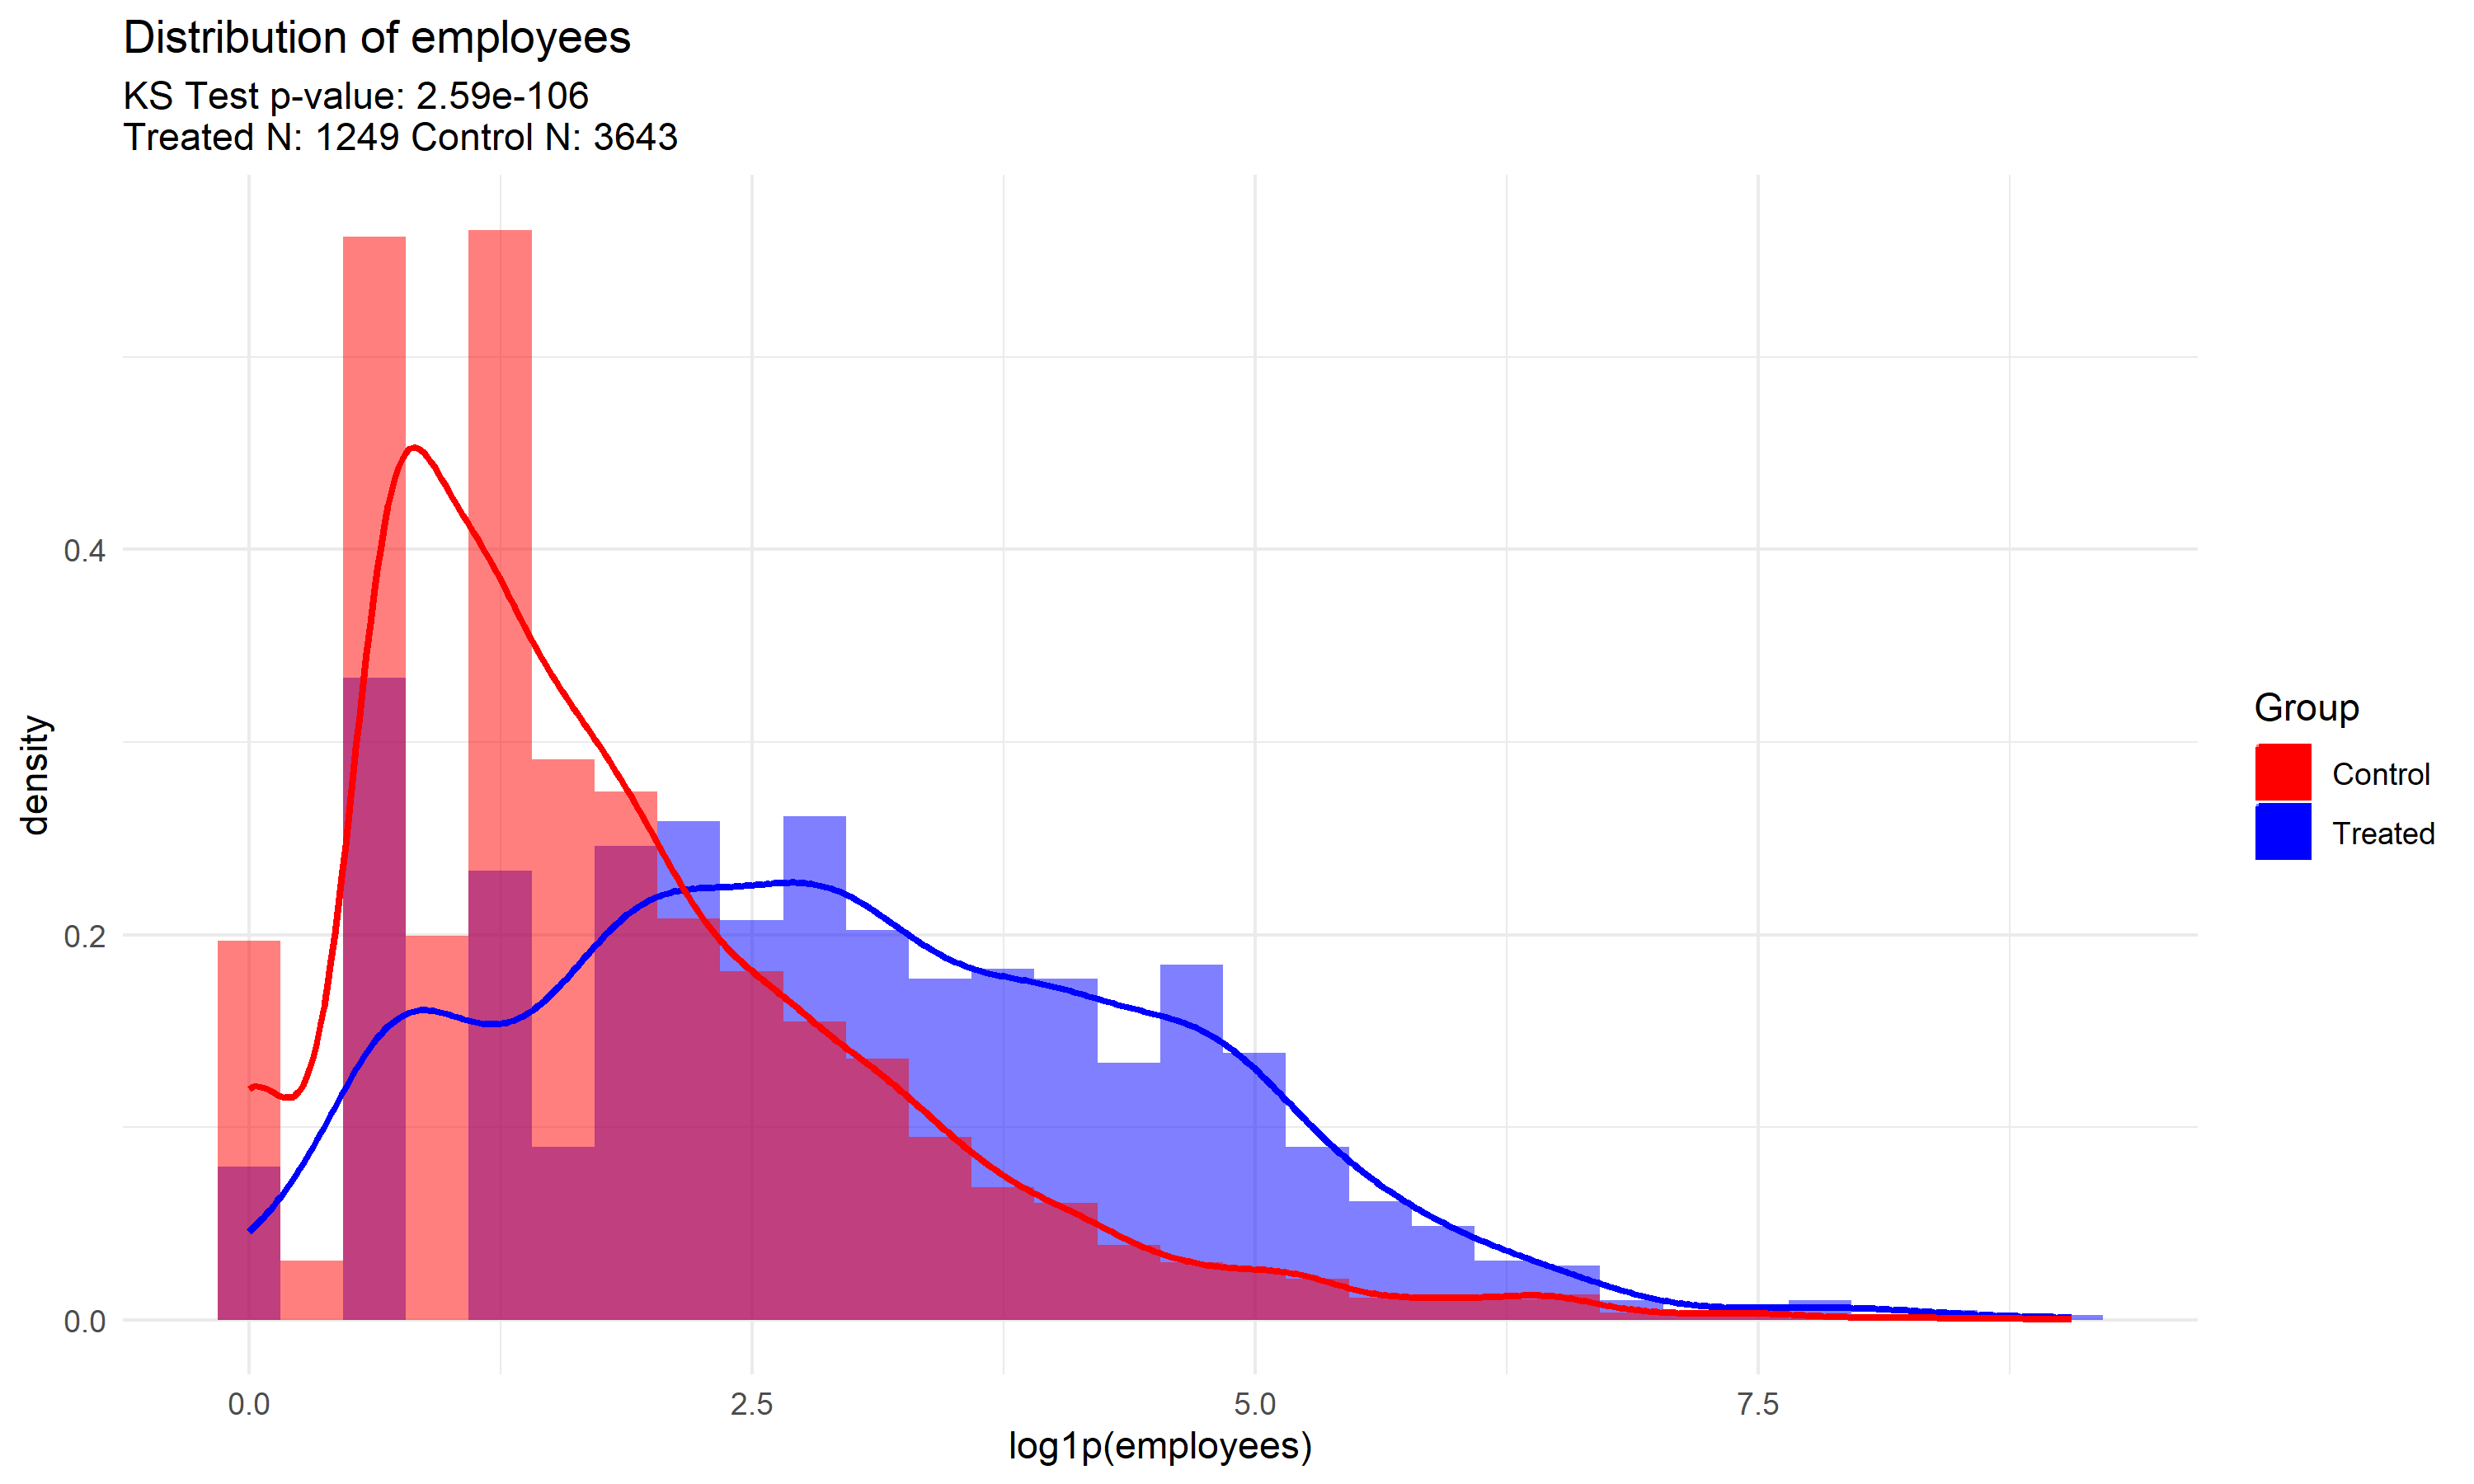
\includegraphics[width=\linewidth]{../Output/distrib_compare_employees_allcountries.png}
        \caption{Employees}
        \label{fig:employees}
    \end{subfigure}
    \vfill
    \begin{subfigure}[b]{0.45\textwidth}
        \centering
        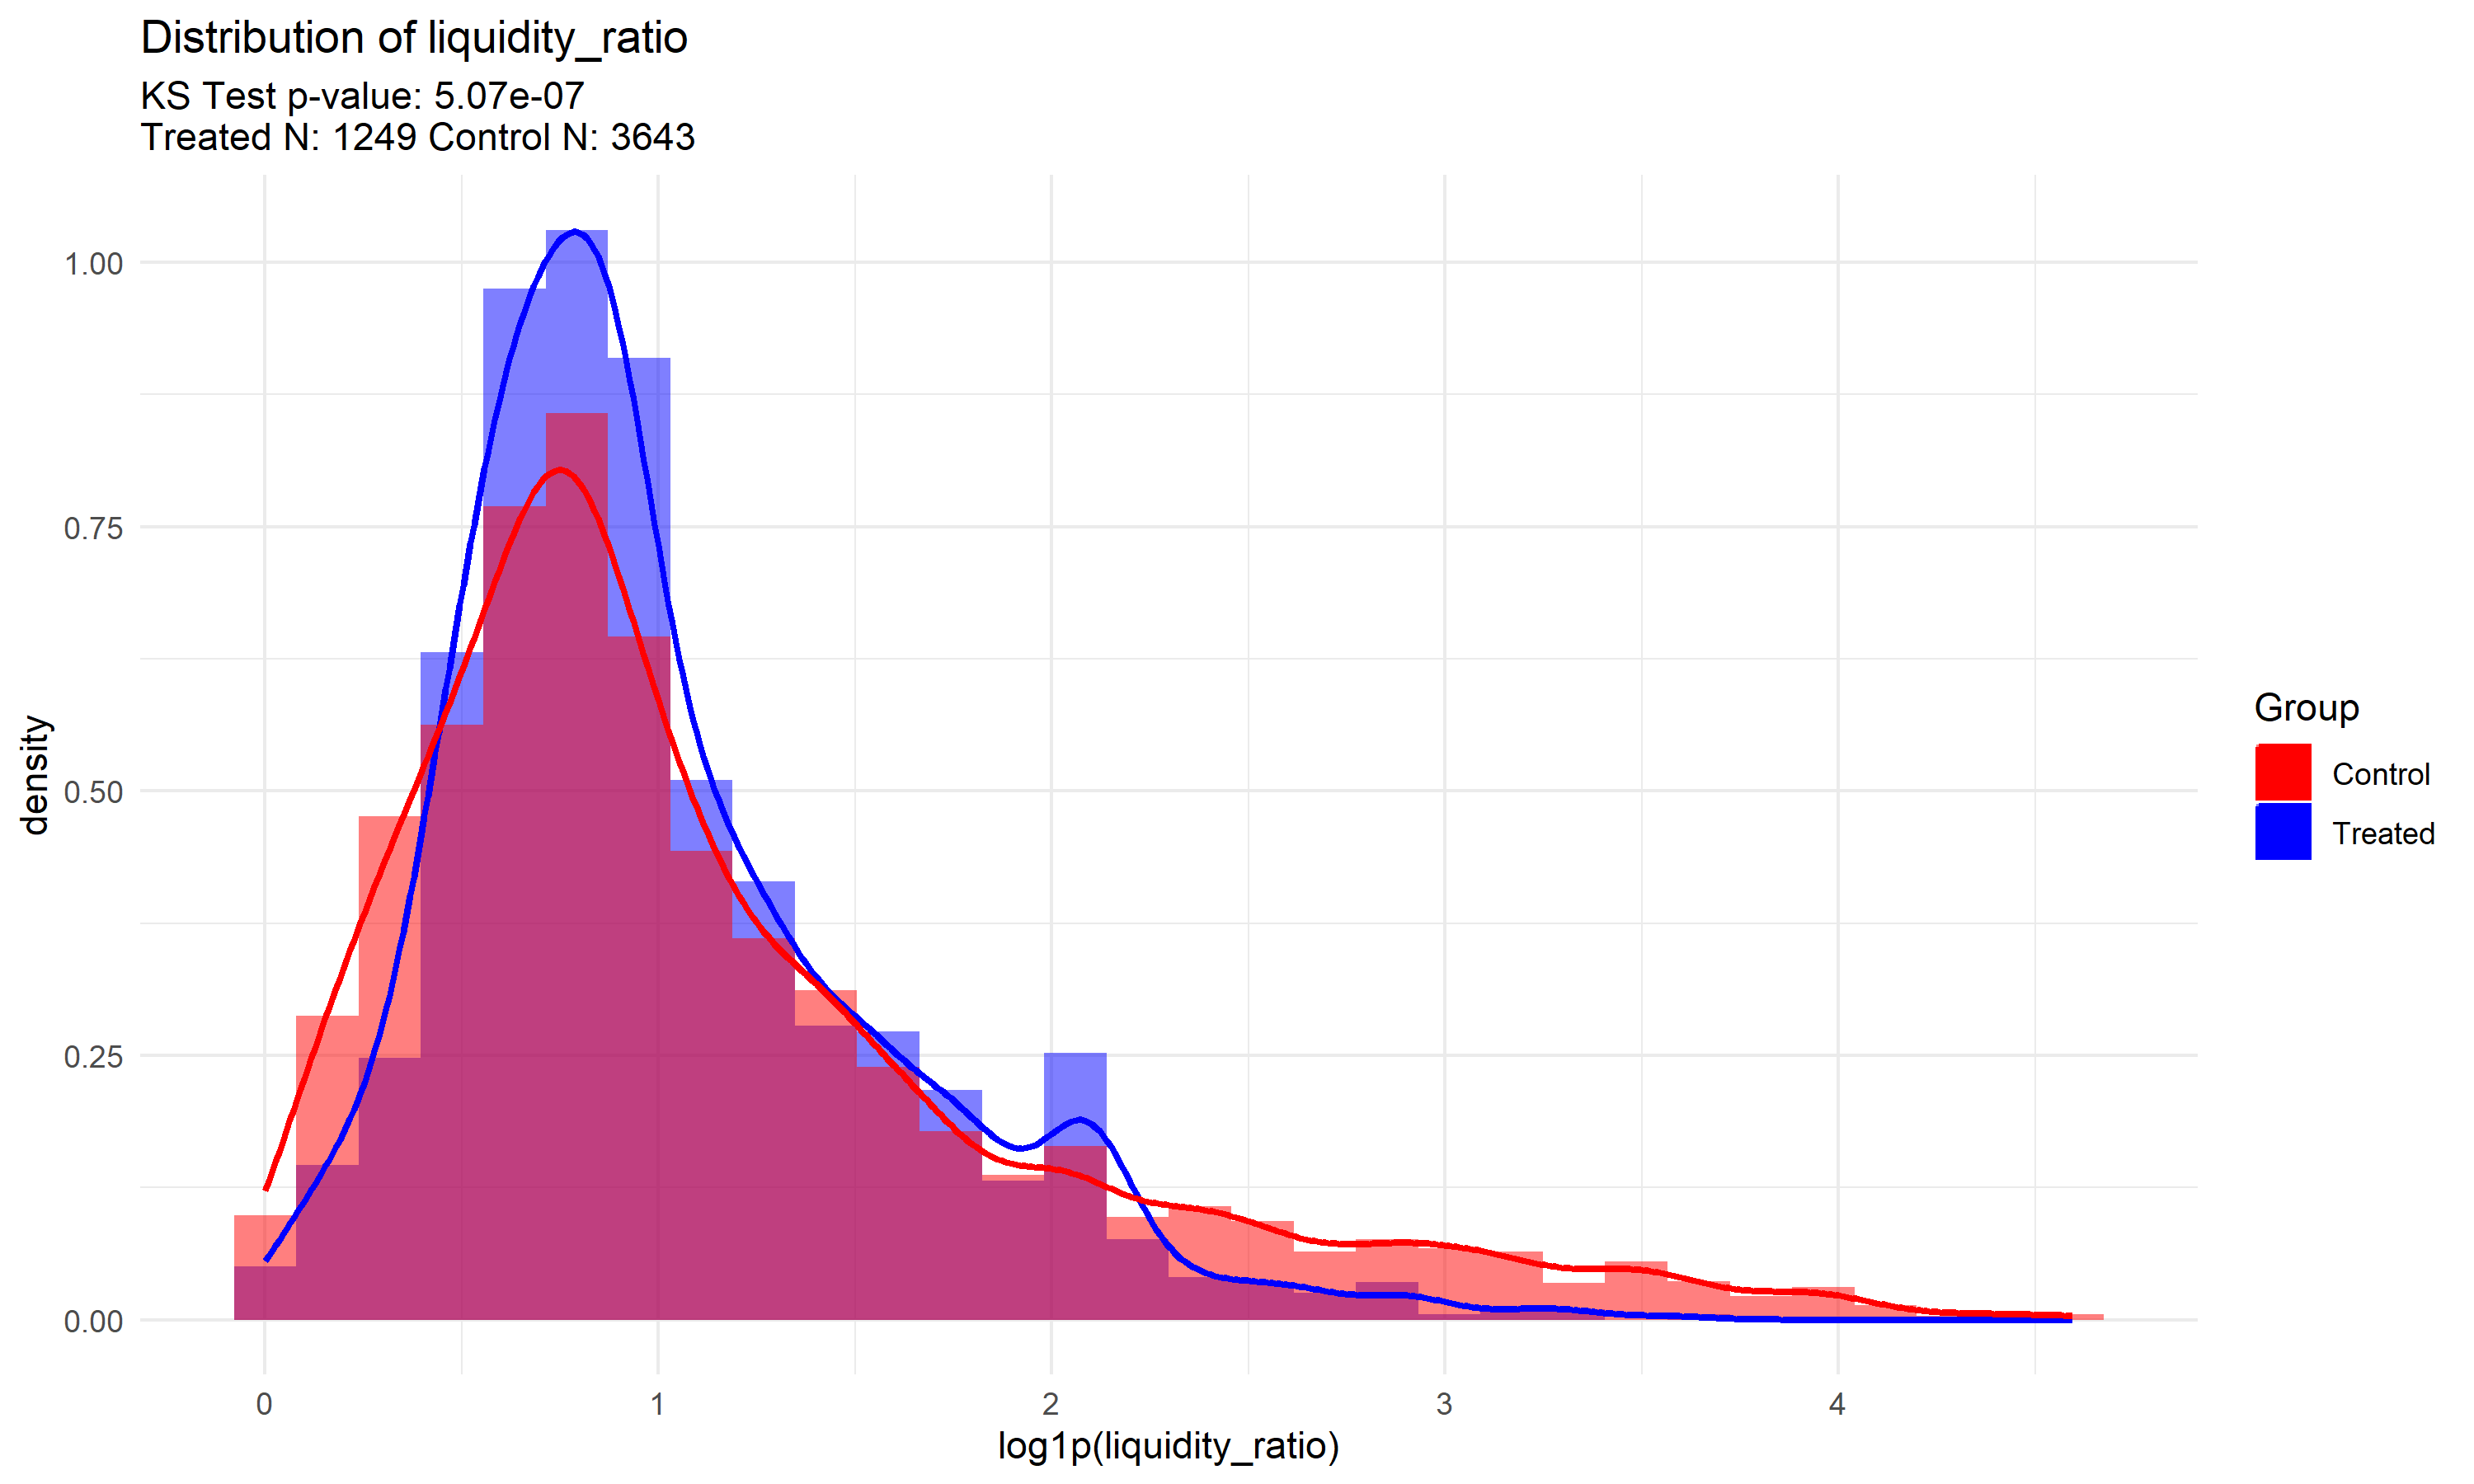
\includegraphics[width=\linewidth]{../Output/distrib_compare_liquidity_ratio_allcountries.png}
        \caption{Liquidity Ratio}
        \label{fig:liquidityratio}
    \end{subfigure}
    \hfill
    \begin{subfigure}[b]{0.45\textwidth}
        \centering
        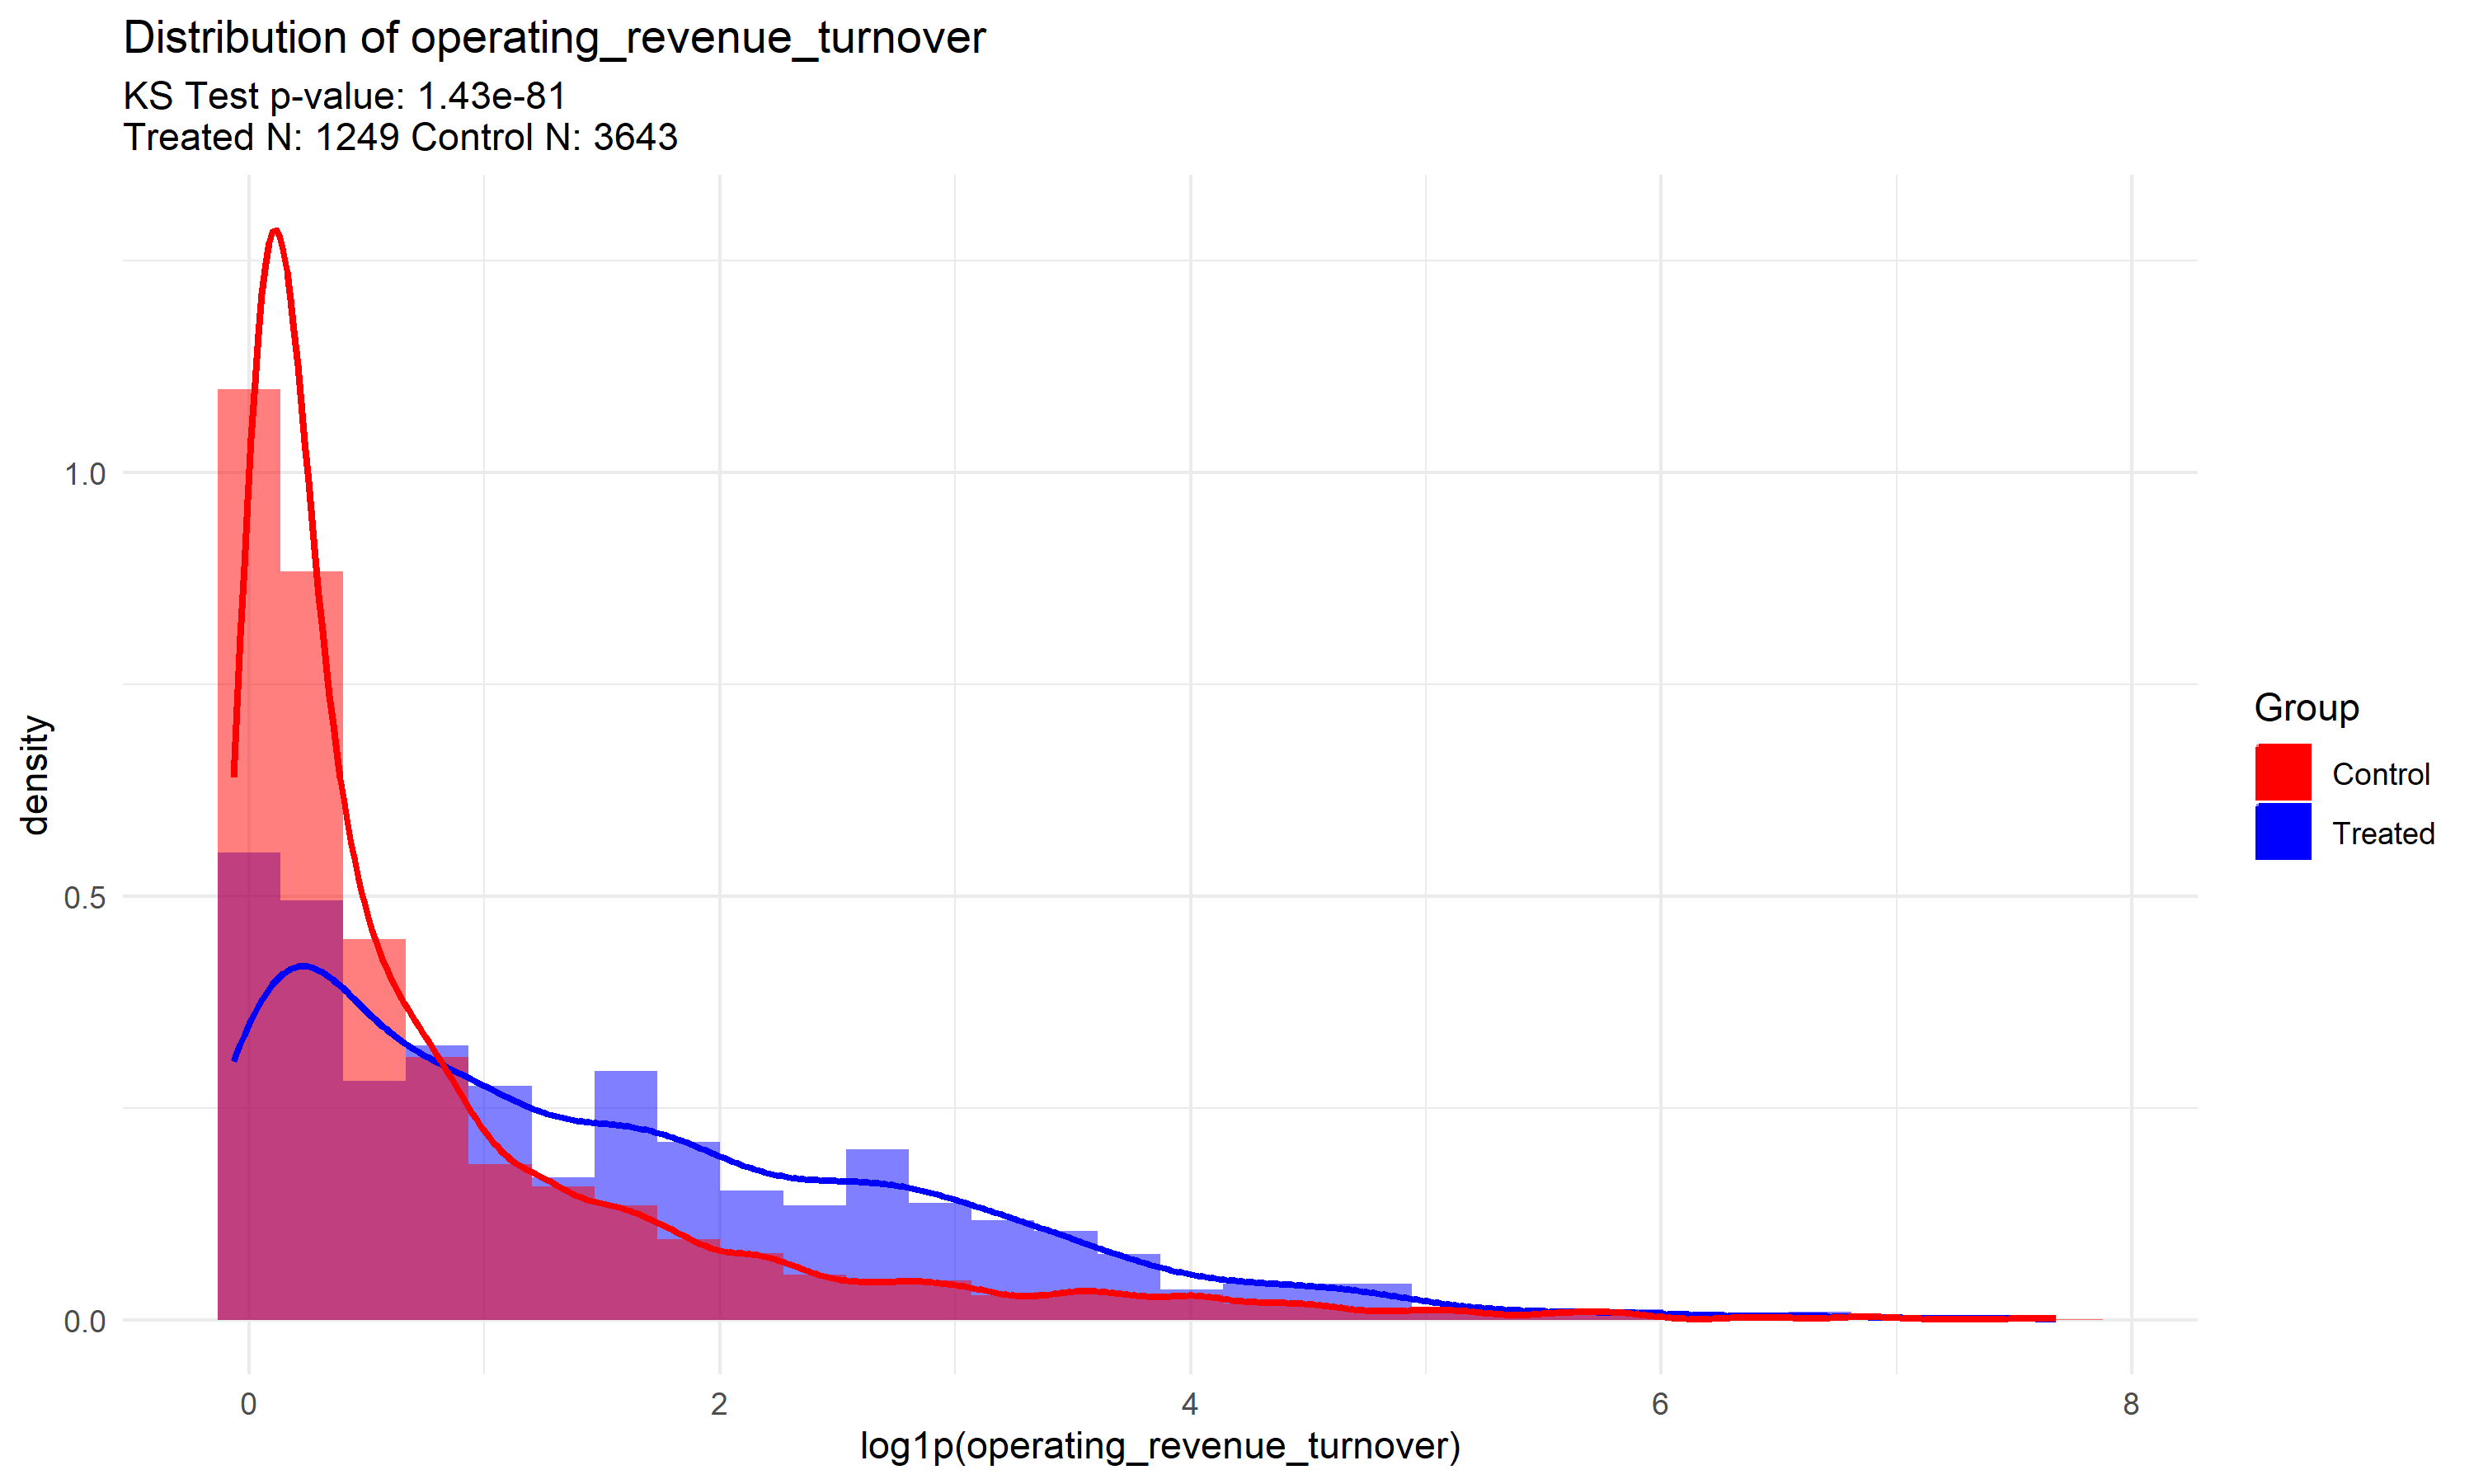
\includegraphics[width=\linewidth]{../Output/distrib_compare_operating_revenue_turnover_allcountries.png}
        \caption{Turnover}
        \label{fig:turnover}
    \end{subfigure}
    \vfill
    \begin{subfigure}[b]{0.45\textwidth}
        \centering
        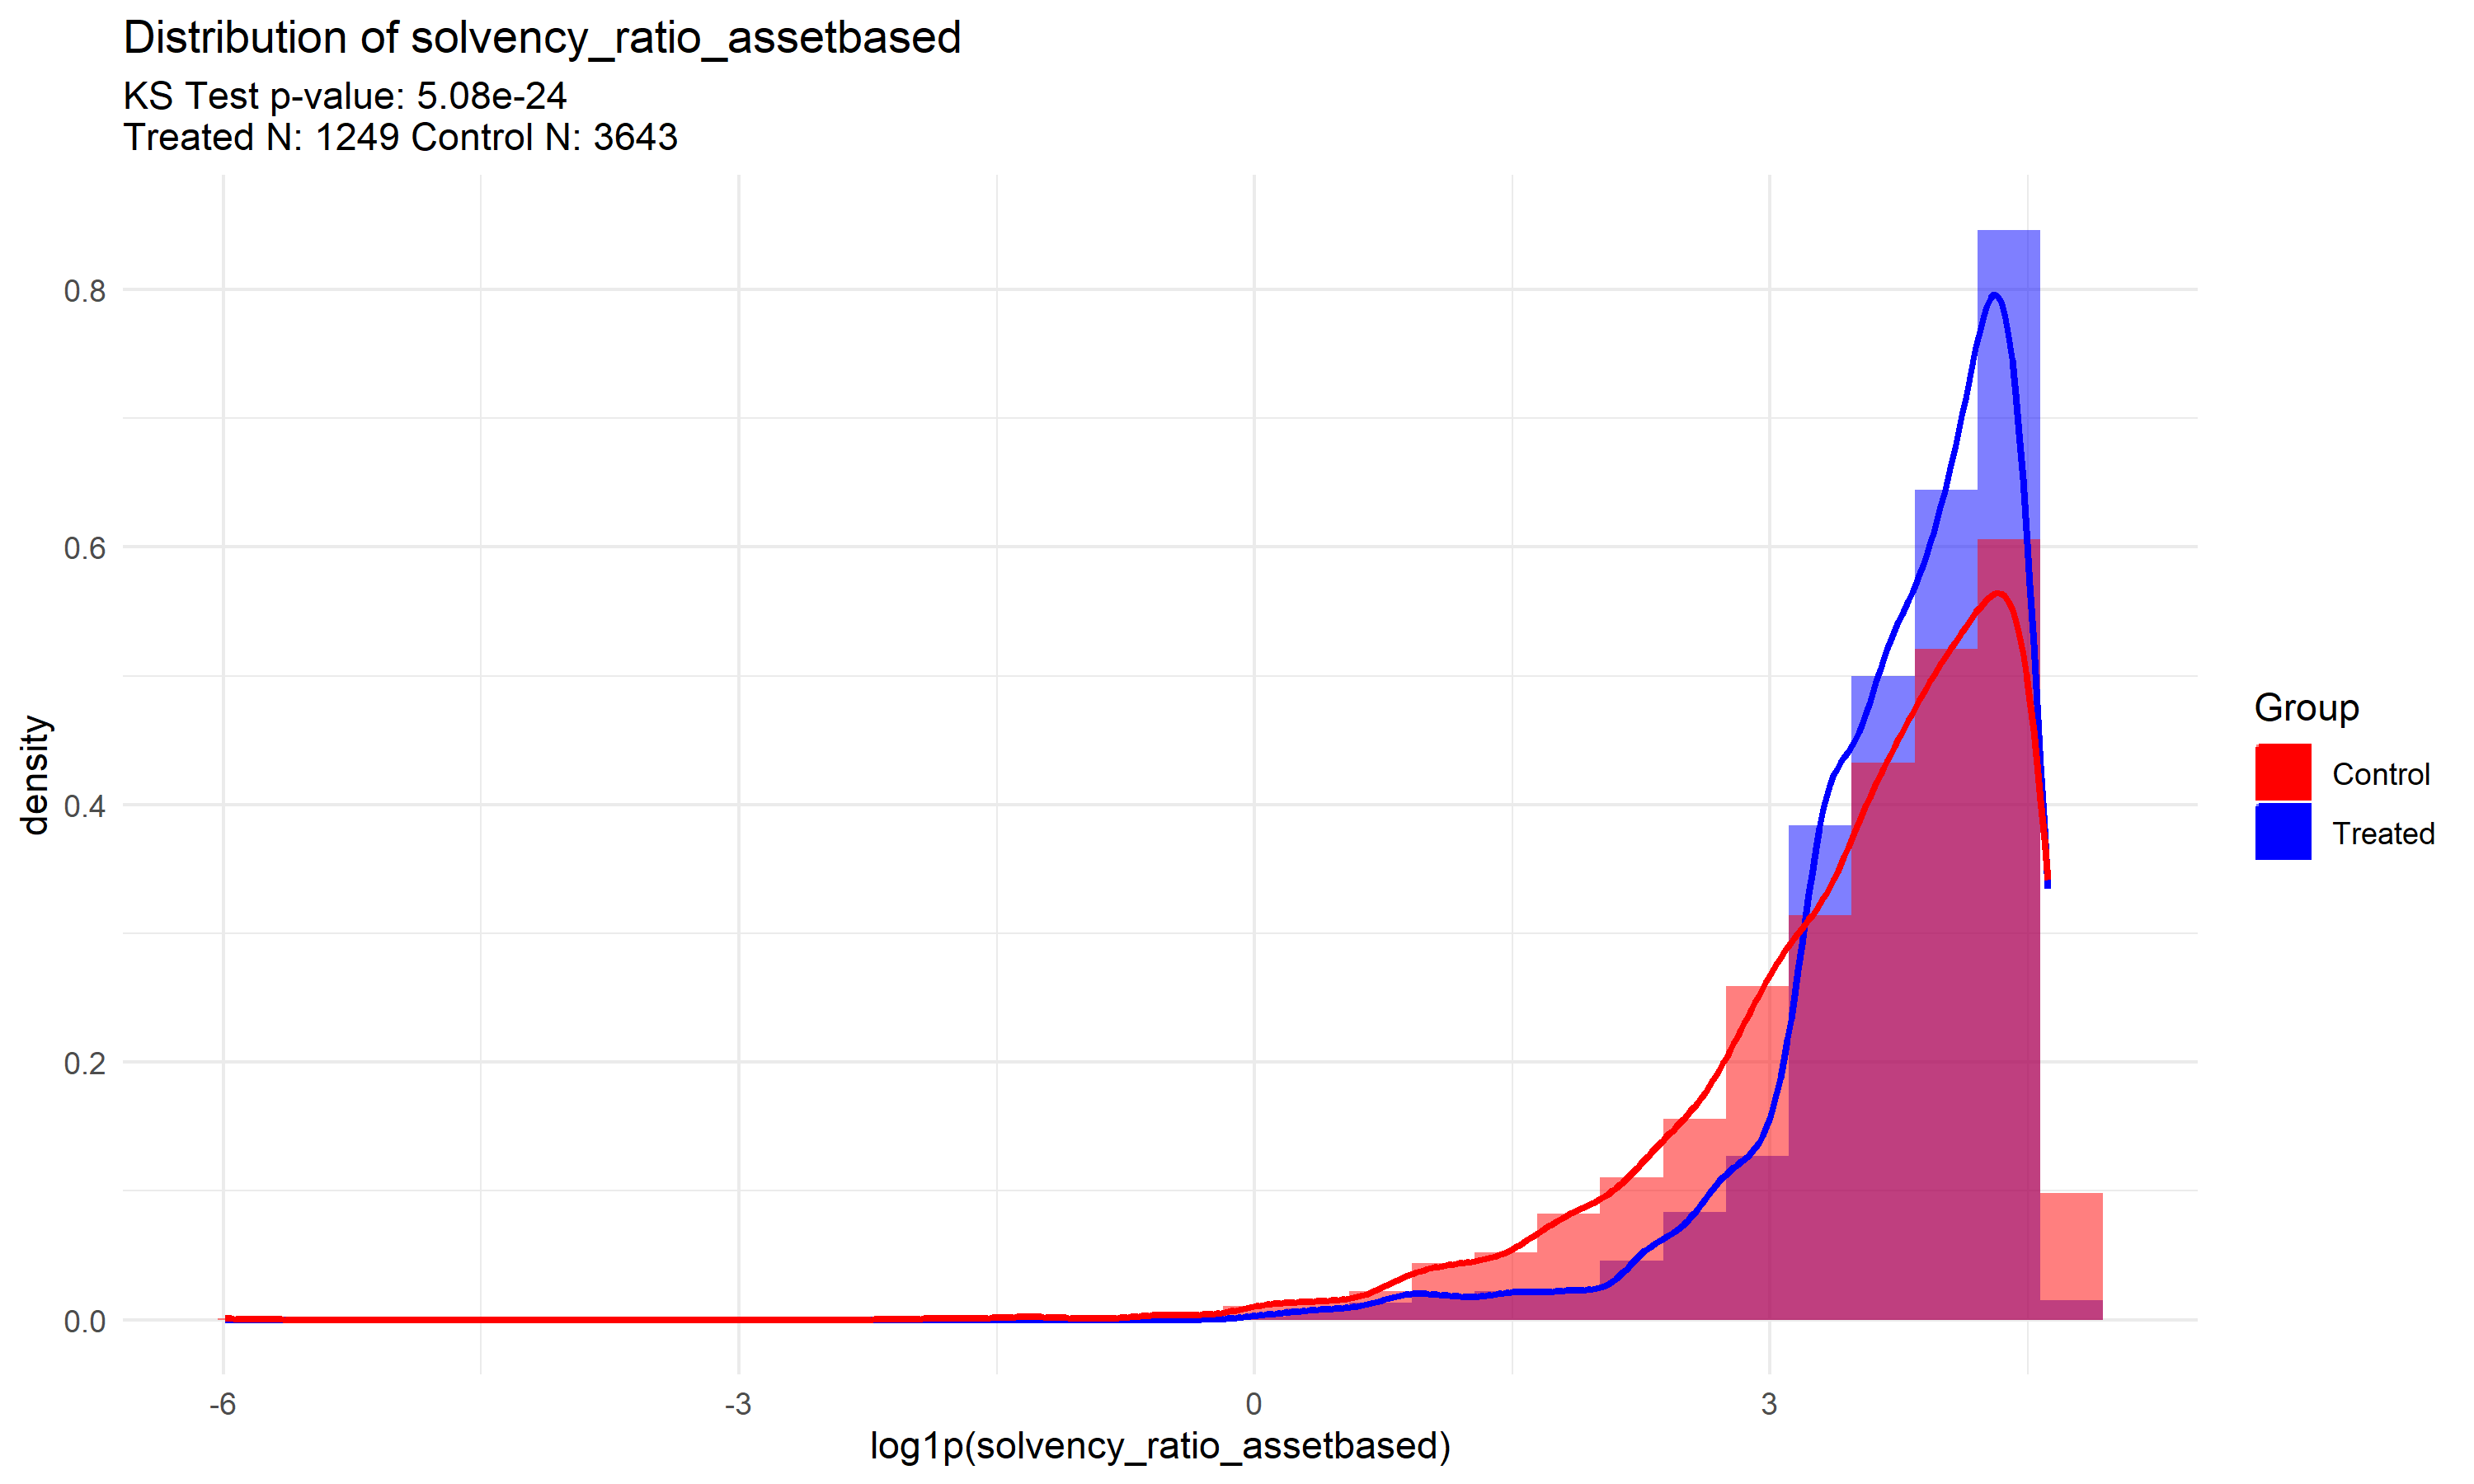
\includegraphics[width=\linewidth]{../Output/distrib_compare_solvency_ratio_assetbased_allcountries.png}
        \caption{Solvency Ratio}
        \label{fig:solvency_ratio}
    \end{subfigure}
    \caption{Distribution Comparisons Across All Countries}
    \label{fig:distribution_comparisons_lotsofvasrs}
\end{figure}

\par I also wanted to compare the sectors in which the firms operate, to see if we can find significant differences there as well. To do that, I divided the firms in the treated and control group using the NACE classification. Industry codes from NACE come as 4-digit codes, but I aggregated them to the 2-digit level to have a more general classification, as well as a more readable graph. Results can be seen in the following figure (as usual, treated firms are in blue and controls in red).

\begin{figure}[h!]
    \centering
    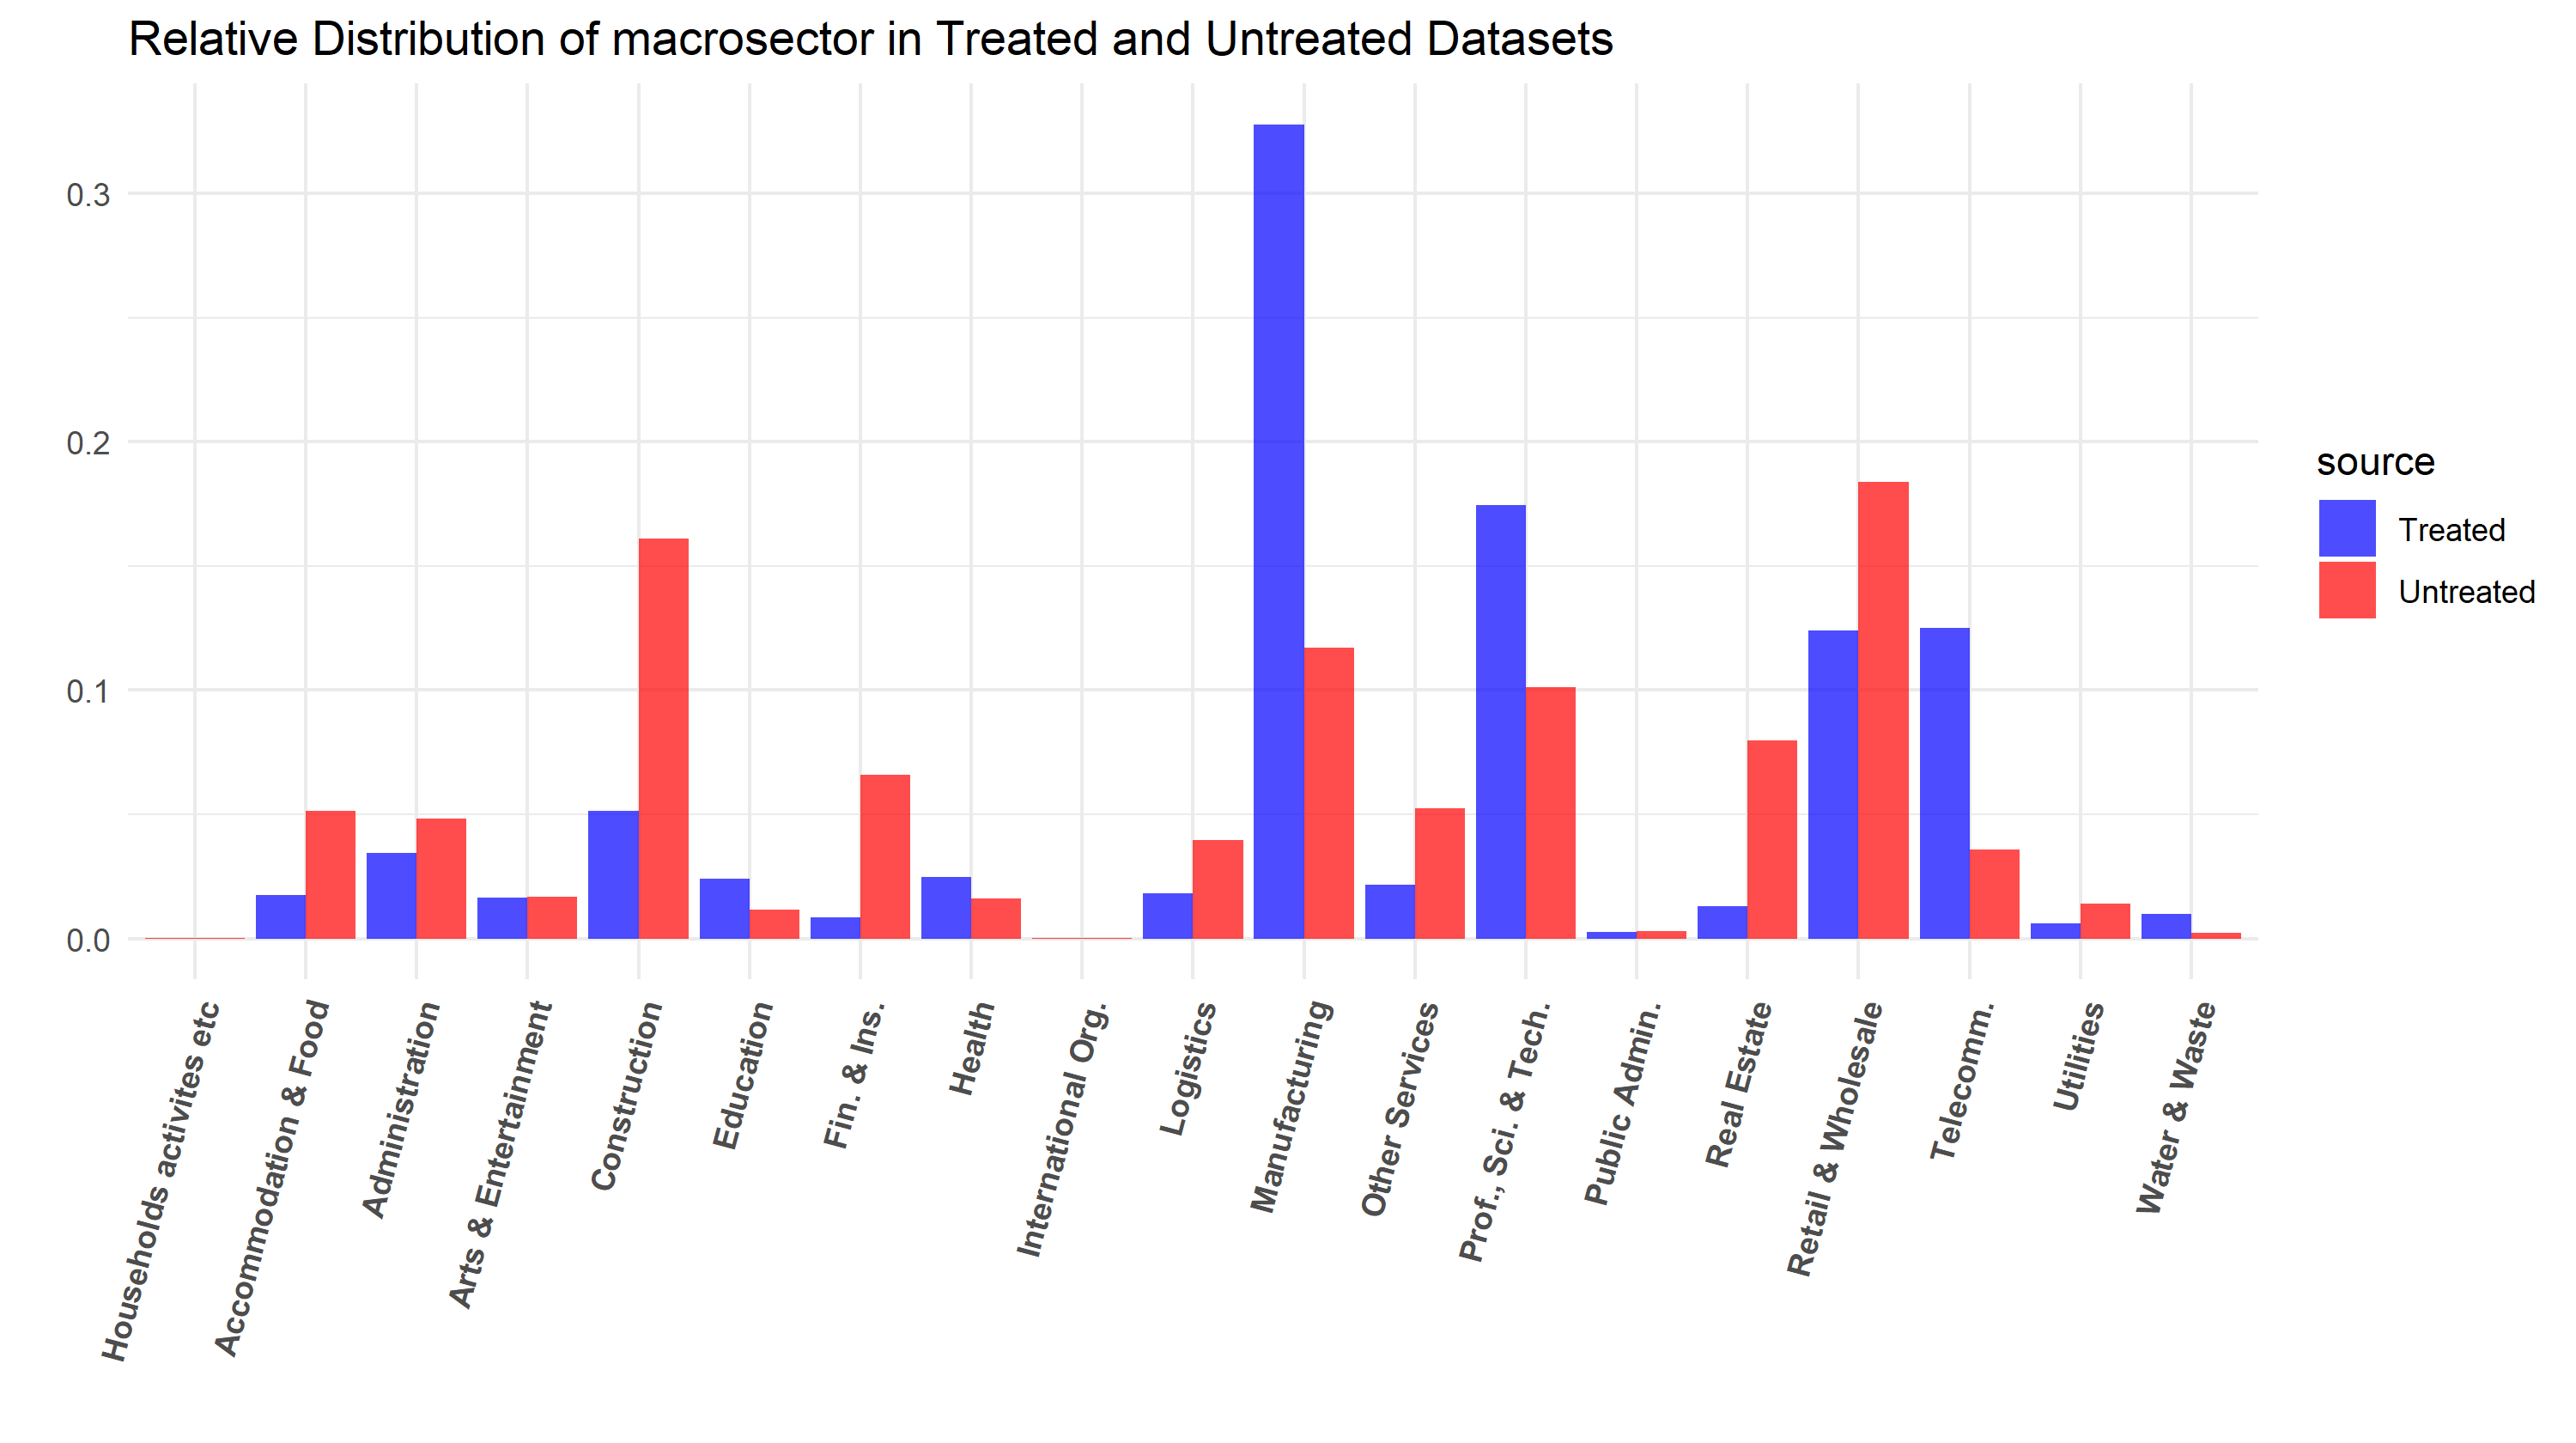
\includegraphics[width=\linewidth]{../Output/macrosectorsplot_compared.png}
    \caption{Comparison of Macro-Sectors in Treated and Control Group}
    \label{fig:distrib_compare_macrosectors_allcountries}
\end{figure}

\par What is immediately noticeable from the graph is how much the sectoral distribution of firms differs between treated and controls. In particular, the macrosectors relating to "Manufacturing", "Professional, scientific and technical activities" and "Information and communication" are overrepresented in the treated group, while "Real estate", "Construction" and "Wholesale and retail trade" are underrepresented.
\par This is probably due to the declared focus of the EDIH initiative on digitalization, and especially on manufacturing technologies. After all, a manufacturing firm can be more easily interested in digitalization since it can profit more from the adoption of these new technologies, while a construction firm may not be as interested. This is an argument for including the macrosector as an independent variable in the regression.

\section{Geocoding, distance and density computation}

\par As I was mentioning in the introductory section of this chapter, I wanted to investigate the effect of the distance of firms from the closest EDIH hub on the probability of participation in the program. 
\par At the start of the process, what I had were addresses, either taken from the DMA survey (for the treated sample) or from the ORBIS database (for the control sample)\footnote{In a small number of cases, ORBIS reported coordinate information as well as the address; in those cases, I took those as being correct, and did not run those observations through the geocoding process}.
\par To get the correct coordinates of the firms, I used the \texttt{geocode} function (part of the \texttt{tidygeocoder} package) in R. This function takes the address string as input and runs the Nominatim API to get coordinate information from the OpenStreetMap database. The function is efficient, but the Nominatim API limits requests to one per second, so I had to time 1 second of sleep for the code for it to work properly. Thus, the process was time-consuming\footnote{Note that the process was done for roughly 18000 firms in the control group, as well as all the firms in the DMA databse, and every EDIH in the database as well. Thus, the geocoding part of the process took some hours to complete}.

\par Once the geocoding loop was done, I had the coordinates of all the firms in the treated and control groups. You can see their geographical distribution in the following map, where treated firms are represented by the red dots, control firms by the light blue dots, and EDIH hubs by the dark blue and dark green dots (the former for EU-financed hubs, the latter for Seal of Excellence hubs).

\begin{figure}[h!]
    \centering
    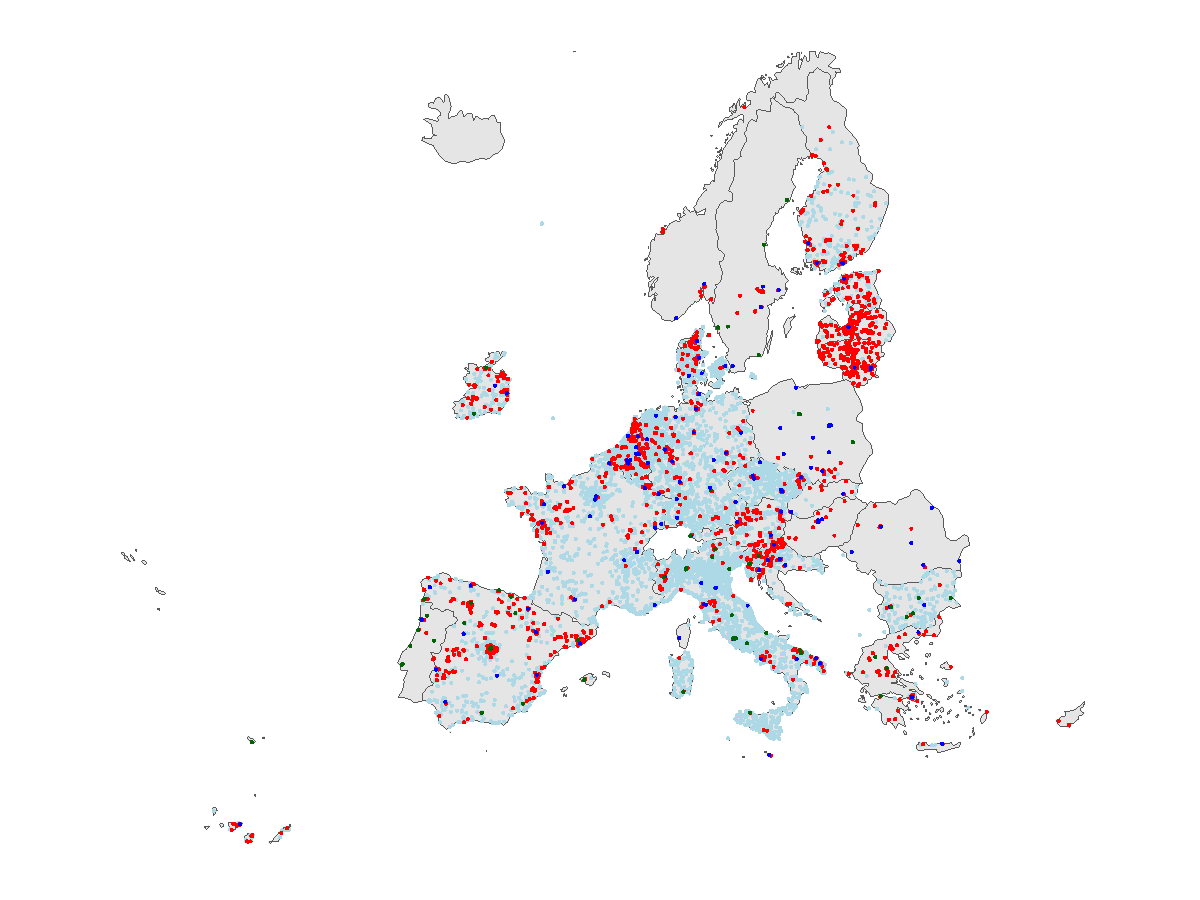
\includegraphics[width=\linewidth,trim={2.8cm 0cm 2.5cm 0.5cm},clip]{../Output/EU_map.pdf}
    \caption{\centering{Map showing the geographical distribution of treated firms (in red), control firms (in light blue) and EDIH hubs (with EU-funded ones in dark blue and regionally/nationally funded ones in dark green) in the whole EU}}
    \label{fig:map_obs_EU}
\end{figure}

\par Already from this map of the whole EU, we can notice some aspects of the analysis we've already discussed. For example, it is clear how the ORBIS coverage is not equally good in each EU country. As a reference, look at the difference in coverage between France and Belgium, or between Italy and Spain. This is important to keep in mind when designing the regression model to use for the analysis, and this is on of the reasons why we will include the country-groups' dummies as an independent variable in the regression.

\par One other thing that we can notice is how the EDIH coverage is not uniform across EU countries, and not even across regions in the same country. For example, let's take a look in detail at Italy, reported individually in the map below.

\begin{figure}[h!]
    \centering
    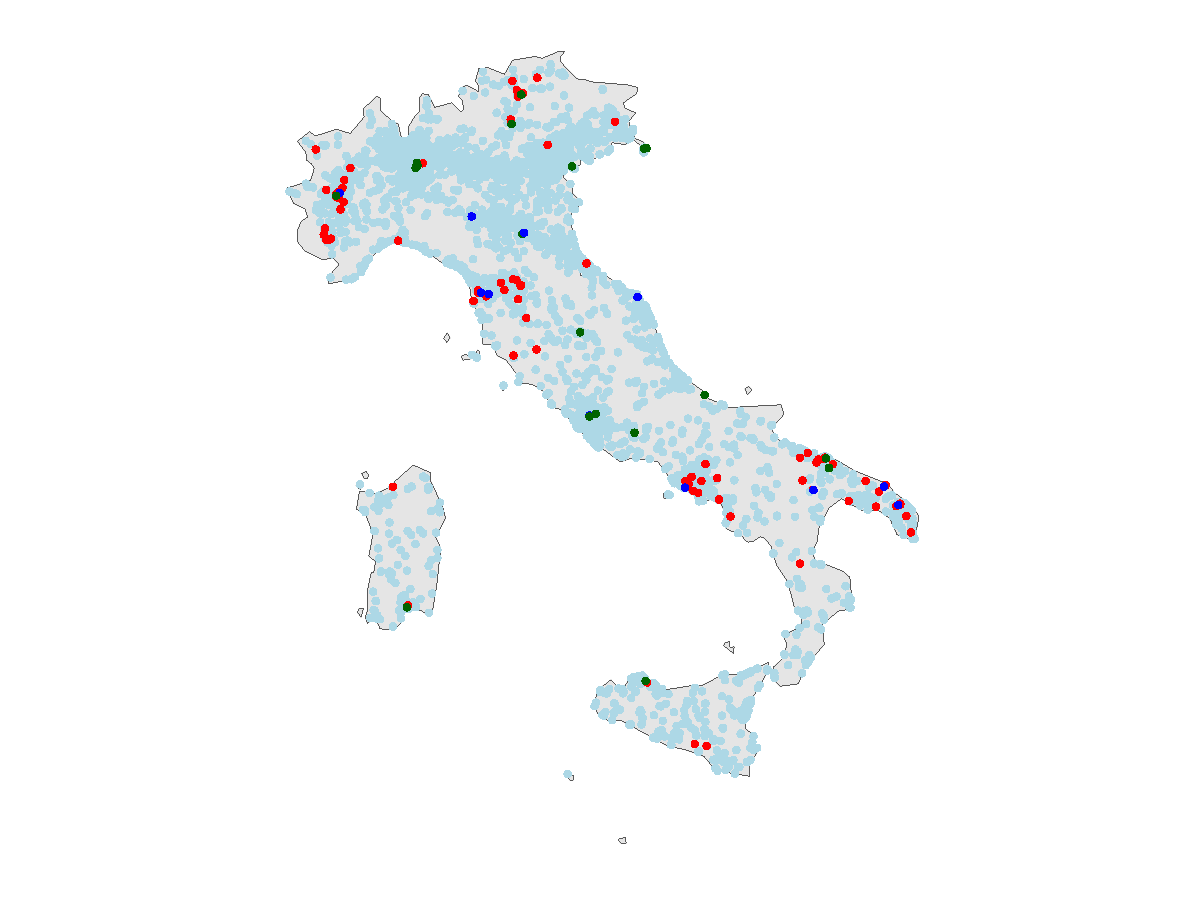
\includegraphics[width=\linewidth]{../Output/IT_map.pdf}
    \caption{\centering{Map showing the geographical distribution of treated firms (in red), control firms (in light blue) and EDIH hubs (with EU-funded ones in dark blue and regionally/nationally funded ones in dark green)} in Italy. All the other individual countries' maps are reported in the Appendix.}
    \label{fig:map_obs_IT}
\end{figure}

\par From this map of firms in Italy, we can see how treated firms are concentrated close to the location of EDIH offices\footnote{One additional note can be made about the fact that EU-financed EDIHs seem to have more treated firms around them w.r.t Seal of Excellence Hubs, which are instead financed through national or regional funds. This fact is not valid only in Italy, and can be an avenue for future research on the effectiveness of the initiative itself. Initial data from the DMA seems in fact to suggest that EU-EDIHs are more active than SoEs. However, please note that this is more likely to be due to a lack of certainty about funding, which is likely delaying start of opeerations for SoEs. Time will tell if their performance will be better in the future.}. This is an initial indication of the negative effect of distance on the probability of accessing the initiative.

\par However, it can also be noted that in many cases treated firms are concentrated in clusters around densely "populated" areas, where also hubs tend to be located. Thus, without including a measure of the "firm density" of the territory in which the firms operate, the effect of proximity to the hubs is likely to get confounded by the effect of being in an area of high firm density\footnote{We can think of firm density as impacting the decision of the firm to participate in the EDIH initiative in many mays. For example, it can be that being surrounded by many firms exposes the firm more to competition, thus making it more imperative to digitalize, and thus seeking help to do so.}.


\par Now that we have coordinates for every firm and EDIH, computing distances is a straightforward (albeit lengthy) process. To get distances, for every firm in the database of treated and controls, I computed its distance with each of the EDIHs in the database, and then chose the closest one. This was done using the \texttt{distHaversine} function from the \texttt{geosphere} package in R. This function takes the 2 sets of coordinates as input and computes the distance between them using the Haversine formula, which is the most accurate way to compute distances on a sphere. 

\par After having computed the distances, I then computed the firm density for each firm. To do this, I utilized the following procedure. For every firm, I first computed the distance between it and every other firm in the database (both treated and controls). Then, I filtered out all firms more distant than a certain threshold\footnote{After a few trials, I settled on a threshold of 5 km, deemed as a good compromise to have an acceptable level of variance in firm density. In fact, a threshold too high would have led to a very high density for every firm, while a threshold too low would have led to a very low density for every firm.}, and counted the number of firms left. You can see a representation of the process in the following figure.

\begin{figure}[ht]
    \centering
    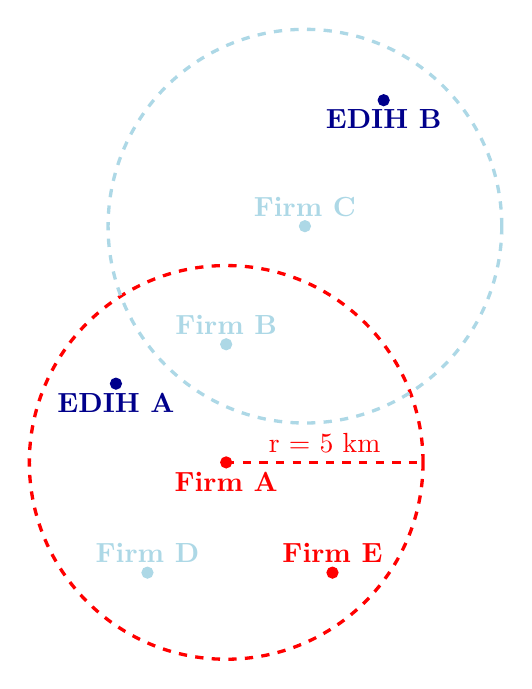
\begin{tikzpicture}
        % Draw a horizontal segmented line to represent the radius
        \draw[red, thick, dashed] (0,0) -- (2.5,0) node[midway, above] {r = 5 km};

        % Draw firms as dots
        \filldraw[red] (0,0) circle (2pt) node[anchor=north] {\textbf{Firm A}};
        \filldraw[lightblue] (0,1.5) circle (2pt) node[anchor=south] {\textbf{Firm B}};
        \filldraw[lightblue] (1,3) circle (2pt) node[anchor=south] {\textbf{Firm C}};
        \filldraw[darkblue] (-1.4,1) circle (2pt) node[anchor=north] {\textbf{EDIH A}};
        \filldraw[darkblue] (2,4.6) circle (2pt) node[anchor=north] {\textbf{EDIH B}};
        \filldraw[lightblue] (-1,-1.4) circle (2pt) node[anchor=south] {\textbf{Firm D}};
        \filldraw[red] (1.35,-1.4) circle (2pt) node[anchor=south] {\textbf{Firm E}};
        
        % Draw a circle around the firms to represent density
        \draw[red, very thick, dashed] (0,0) circle (2.5cm);

        \draw[lightblue, very thick, dashed] (1,3) circle (2.5cm);
    \end{tikzpicture}
    \caption{\centering{Diagram showing the criteria for computing firm density. In the image, Firm A has a firm density of 3, while Firm C has a firm density of 1.}}
    \label{fig:firm_density_glyph}
\end{figure}

\par In the diagram you can see how Firm A has a firm density of 3, as firms B, D, and E all fall inside of the 5km-radius circle around Firm A (while EDIH offices are not counted as firms). On the other hand, Firm C has a firm density of only 1, since Firm B is the only one inside the 5km-radius circle around Firm C (and again, EDIH offices are not counted as firms). From the diagram you can also see how in the computation of firm density, both treated and control firms are taken into account.

\par Thus, the designed measure of firm density can be considered as an accurate proxy of the density of firms on the EU territory, at least when the ORBIS bias is taken into account.

\par Now that we have computed both firm distance and density measures, we can add them to the initial treated-control comparison, to see how they differ between the two groups, as seen in the following tables.




\begin{figure}[ht]
    \centering
    \begin{subfigure}[b]{0.45\textwidth}
        \centering
        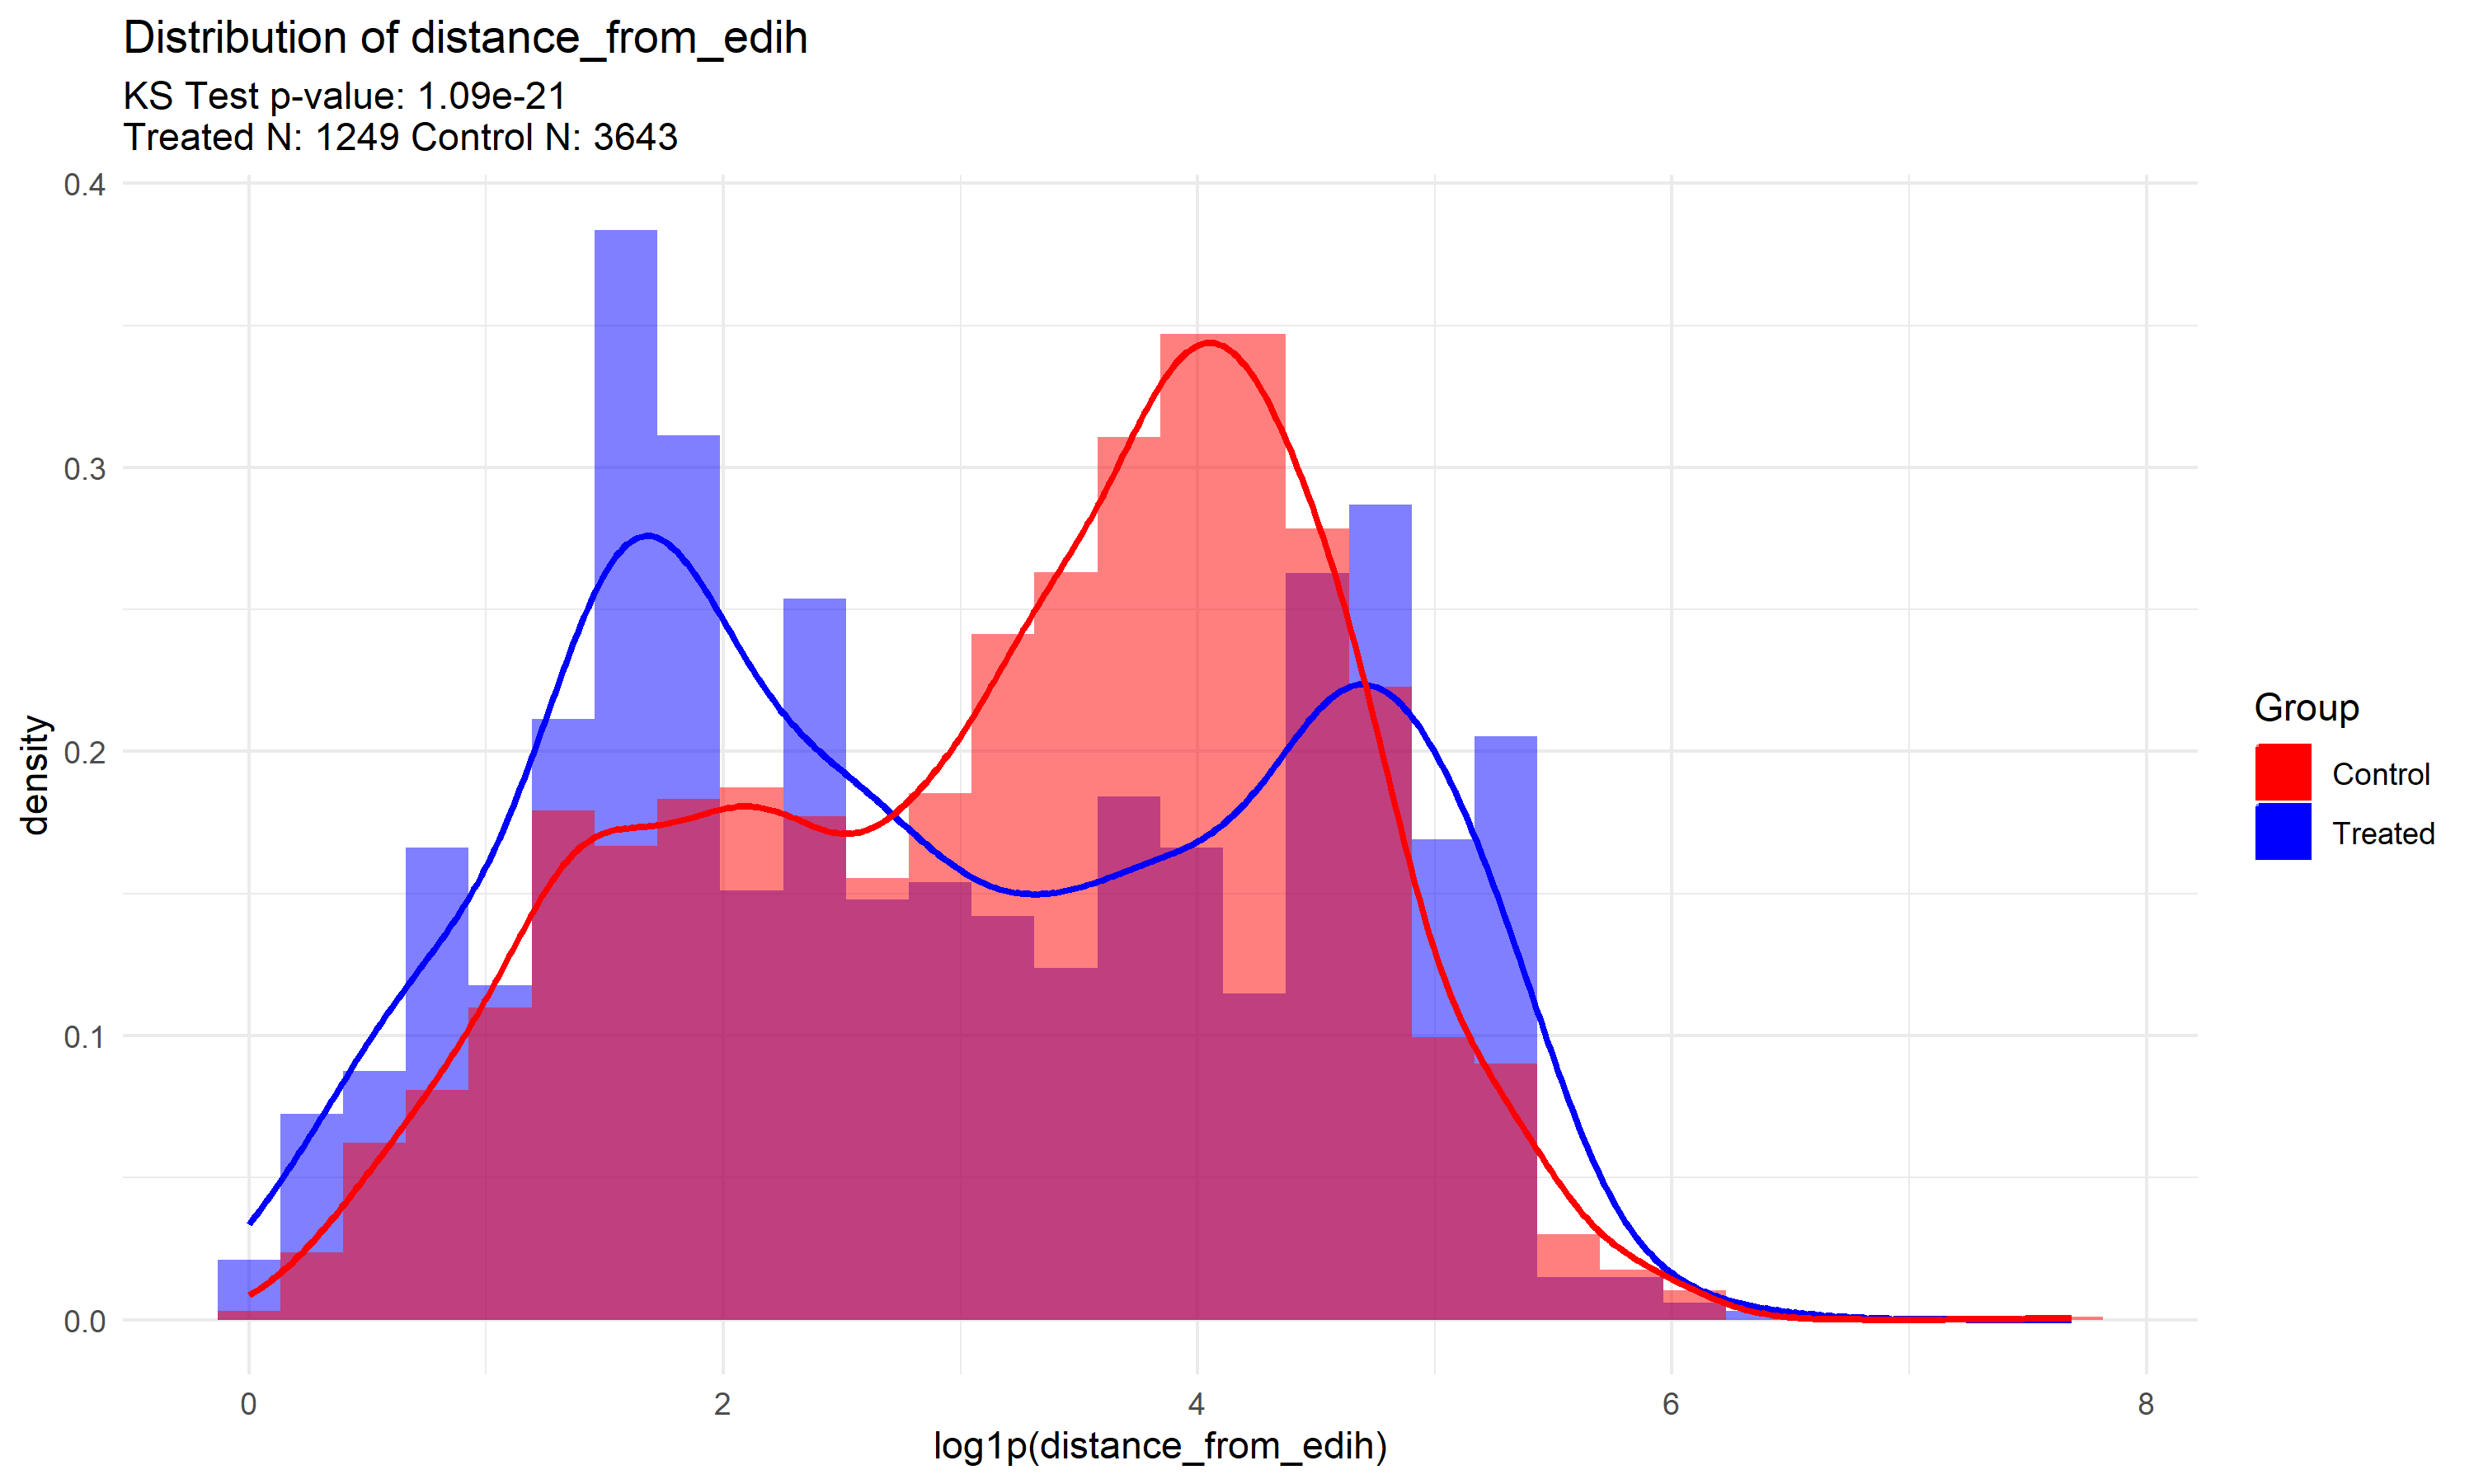
\includegraphics[width=\linewidth]{../Output/distrib_compare_distance_from_edih_allcountries.png}
        \caption{Distance from closest EDIH}
        \label{fig:distance_from_edih}
    \end{subfigure}
    \hfill
    \begin{subfigure}[b]{0.45\textwidth}
        \centering
        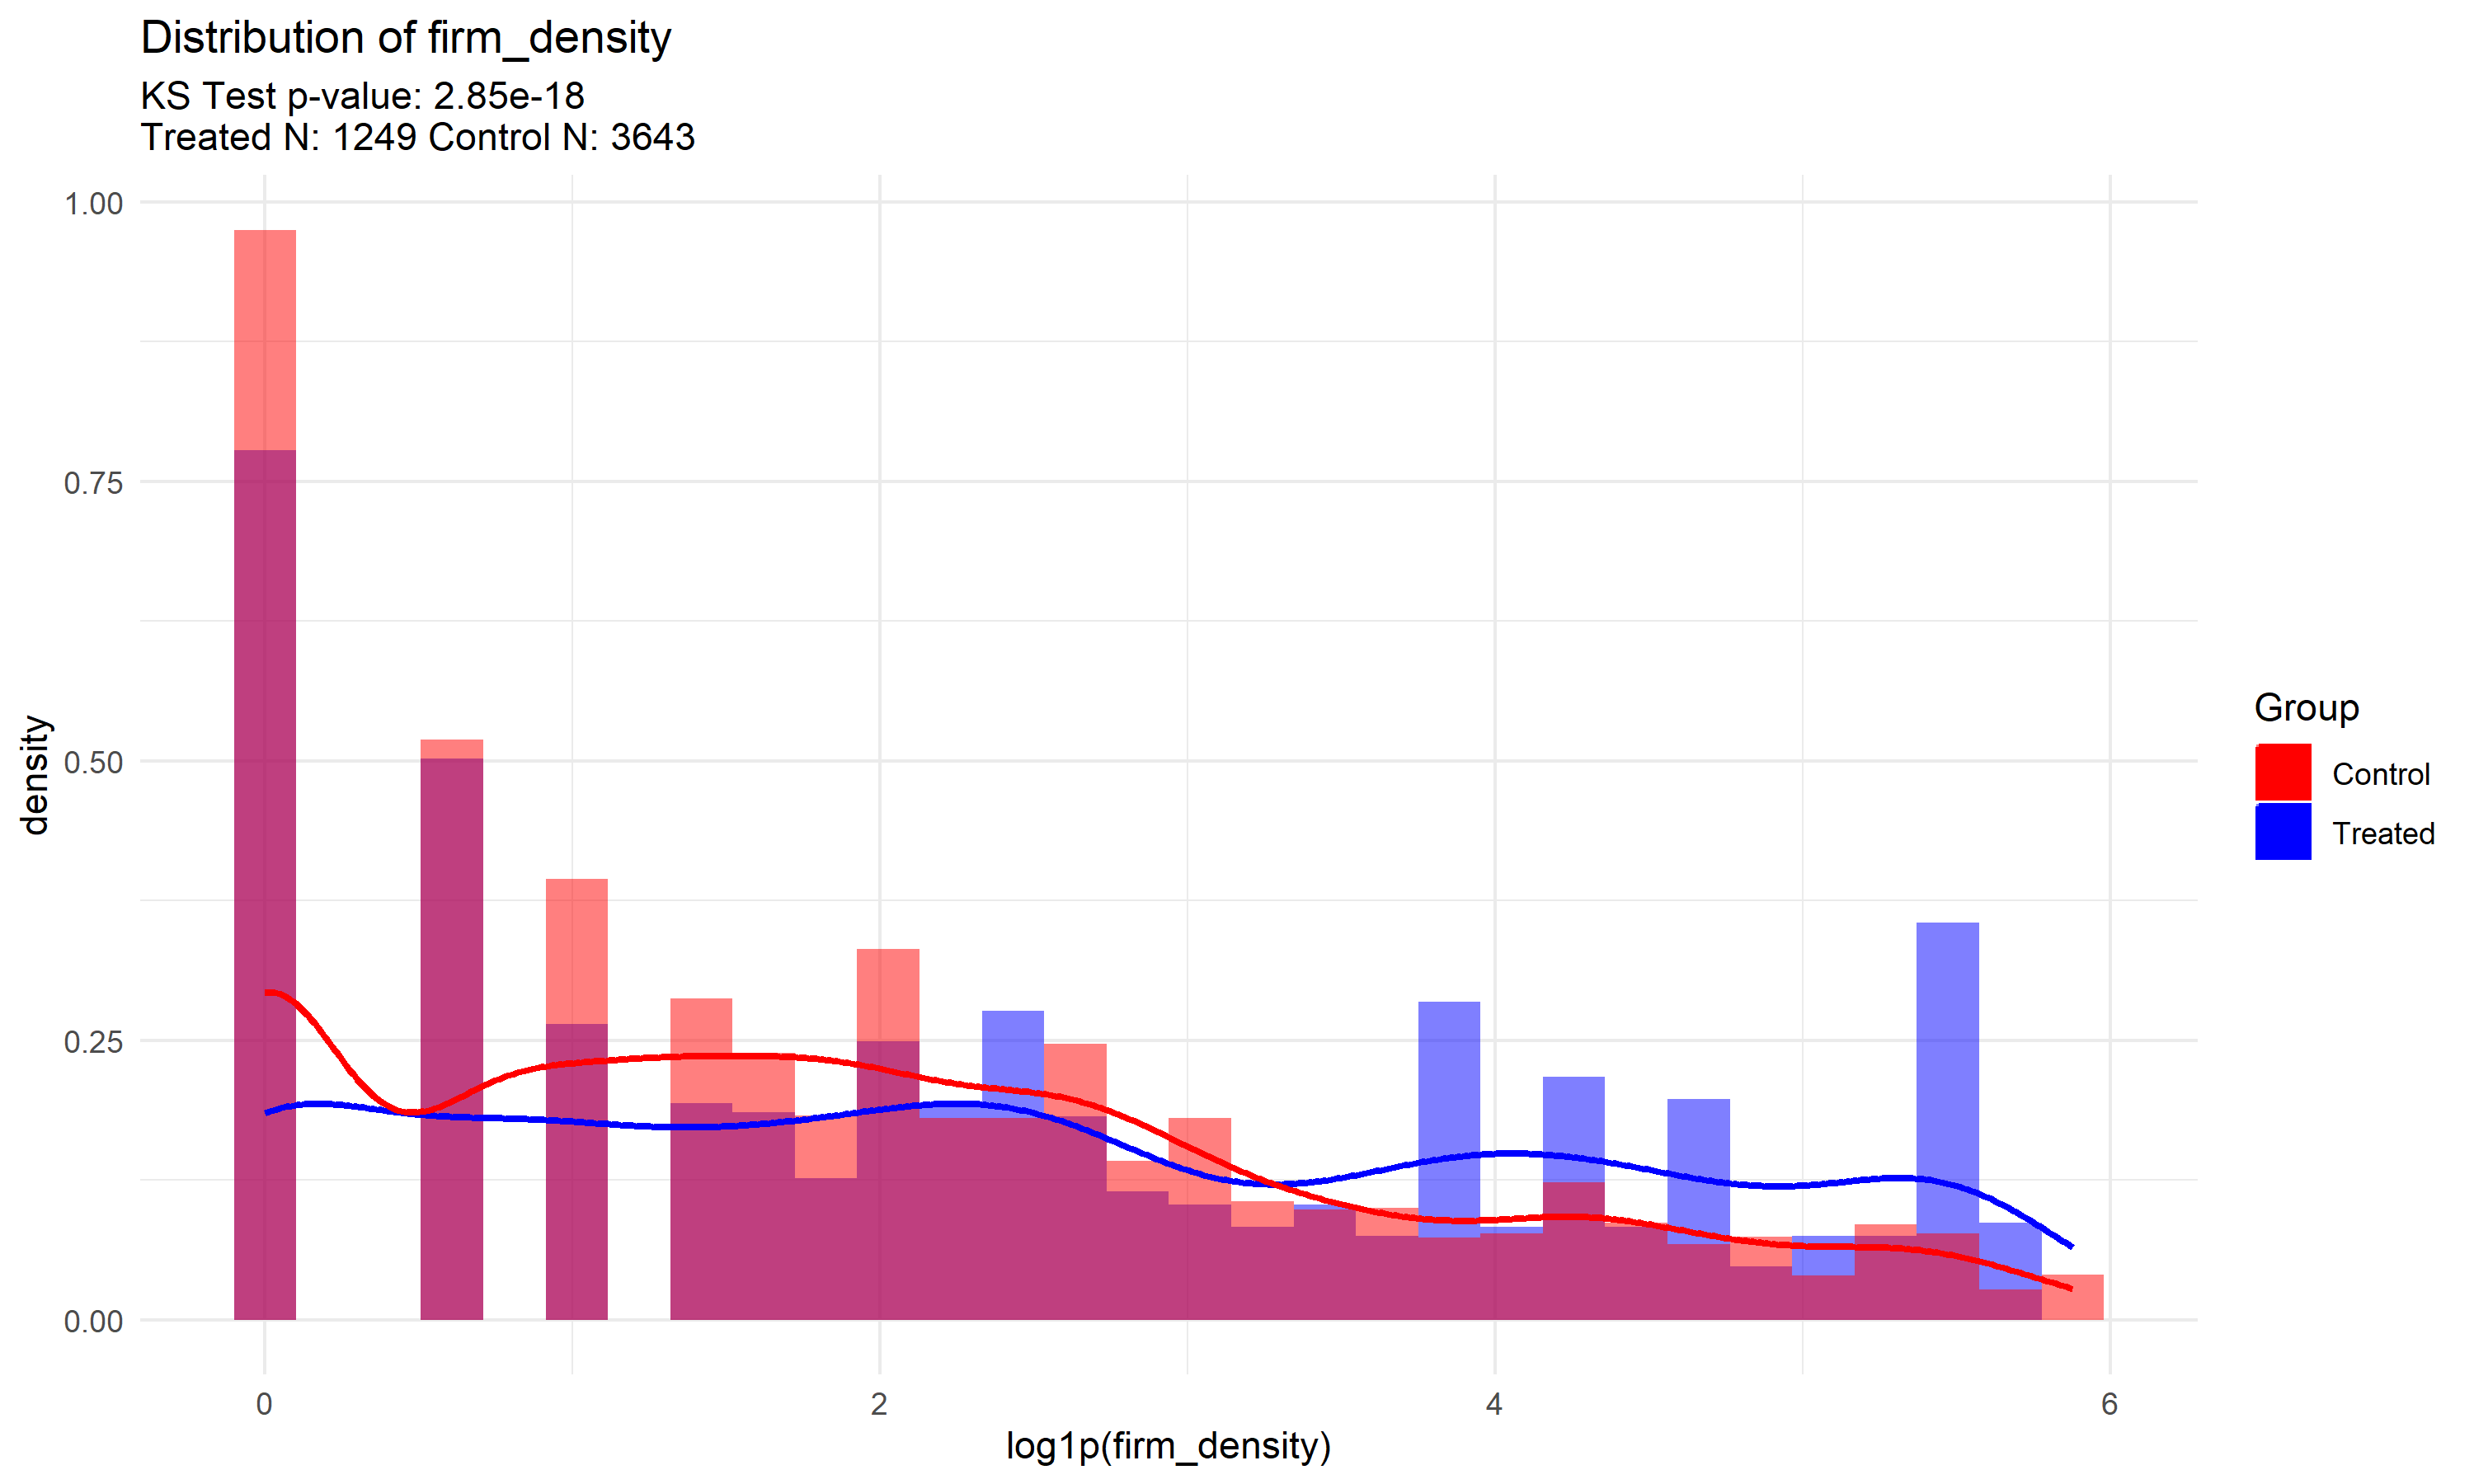
\includegraphics[width=\linewidth]{../Output/distrib_compare_firm_density_allcountries.png}
        \caption{Firm Density}
        \label{fig:firm_density}
    \end{subfigure}
    \caption{Distribution Comparisons of distance and firm density across all Countries}
    \label{fig:distribution_comparisons}
\end{figure}

\par In both cases, we can see from the results of the KS-tests that the treated and control groups hail from different distributions. In addition, it seems that treated firms are on average closer to the EDIH hubs, are also located in areas with higher firm density. This is an additional indication that the spatial dimension is significant in understanding the drivers of firms' participation to the EDIH initiative.





\section{Regression Model and Results}

\par As previously mentioned in the sections above, to analyze the drivers of participation in the EDIH initiative, I have run a probit regression model. The model includes various firm-level characteristics as independent variables, and the dependent variable is a dummy variable indicating whether the firm participated in the EDIH initiative. The model is specified as follows:

\begin{equation}
    \begin{split}
        D_{i}(\text{Treated}_{i} = 1) = \beta_{0} &+ \beta_{1} \text{Distance}_{i} + \beta_{2} \text{Firm Density}_{i} \\
        &+ \beta_{3} \text{Sector}_{i} + \beta_{4} \text{Tech Level}_{i} \\
        &+ \beta_{5} \text{Turnover}_{i} + \beta_{6} \text{Employees}_{i} \\
        &+ \beta_{7} \text{Liquidity Ratio}_{i} + \beta_{8} \text{Solvency Ratio}_{i} \\
        &+ \beta_{9} \text{Country Group}_{i} + \varepsilon_{i}
    \end{split}
\end{equation}


\par Where the dependent variable is a dummy indicating participation to the program, Distance and Firm Density are defined as above, Sector is a variable indicating the type of sector to which the firm belongs (either Manufacturing, Services or Other, with the baseline being Other). Tech Level is a variable indicating the level of technological intensity of the sector in which the firm is operating, according to the OECD taxonomy defined in \cite{oecdclassification}; in this case, the baseline is represented by the lowest level of the OECD taxonomy. Turnover, Employees, Liquidity Ratio and Solvency Ratio are all firm-level variables coming from the ORBIS database. More specifically, turnover serves as a proxy for firm profitability, employees proxies for firm size (total assets was excluded to being too collinear with employees), while liquidity ratio and solvency ratio are proxies for the financial wellbeing of the firm. Country Group is a dummy indicating the group to which the country in which the firm is located belongs; the groups are Central Europe, Southern Europe, Baltics, Benelux, Balkans, and Western Europe, with the baseline being Central Europe.

\par In addition to running this regression on the whole sample, I also ran it on the subsamples of firms in the Manufacturing sector, in the Services sector, and in the Other sector, to see if results were particularly driven by one of these macrosectors of the economy.

\par In the following table, you can first see the results of the regression analysis on the whole sample, first without the spatial dimensions (distance and firm density), and then with them included. The results are reported as coefficients, with the standard errors in parentheses.


% Table created by stargazer v.5.2.3 by Marek Hlavac, Social Policy Institute. E-mail: marek.hlavac at gmail.com
% Date and time: mer, apr 09, 2025 - 18:31:44
\begin{table}[!htbp] \centering 
  \caption{} 
  \label{} 
\begin{tabular}{@{\extracolsep{5pt}}lccc} 
\\[-1.8ex]\hline 
\hline \\[-1.8ex] 
\\[-1.8ex] & \multicolumn{3}{c}{treated} \\ 
 & w/o Dist & w/ Dist & w/ Dist and Dens \\ 
\hline \\[-1.8ex] 
 distance\_from\_edih &  & $-$0.002$^{***}$ & $-$0.002$^{***}$ \\ 
  &  & (0.0004) & (0.0004) \\ 
  & & & \\ 
 firm\_density &  &  & 0.001$^{***}$ \\ 
  &  &  & (0.0005) \\ 
  & & & \\ 
 sector\_typeManufacturing & 0.328$^{***}$ & 0.337$^{***}$ & 0.361$^{***}$ \\ 
  & (0.103) & (0.103) & (0.103) \\ 
  & & & \\ 
 sector\_typeServices & 0.269$^{***}$ & 0.245$^{***}$ & 0.222$^{***}$ \\ 
  & (0.074) & (0.074) & (0.074) \\ 
  & & & \\ 
 tech\_levelHigh & 1.260$^{***}$ & 1.233$^{***}$ & 1.216$^{***}$ \\ 
  & (0.181) & (0.182) & (0.183) \\ 
  & & & \\ 
 tech\_levelMedium & 0.783$^{***}$ & 0.766$^{***}$ & 0.749$^{***}$ \\ 
  & (0.143) & (0.144) & (0.144) \\ 
  & & & \\ 
 tech\_levelMedium-High & 1.592$^{***}$ & 1.554$^{***}$ & 1.539$^{***}$ \\ 
  & (0.088) & (0.089) & (0.089) \\ 
  & & & \\ 
 tech\_levelMedium-Low & 0.774$^{***}$ & 0.745$^{***}$ & 0.723$^{***}$ \\ 
  & (0.070) & (0.071) & (0.072) \\ 
  & & & \\ 
 operating\_revenue\_turnover & $-$0.0004 & $-$0.0004 & $-$0.0004 \\ 
  & (0.0005) & (0.0005) & (0.0005) \\ 
  & & & \\ 
 employees & 0.768$^{***}$ & 0.749$^{***}$ & 0.741$^{***}$ \\ 
  & (0.165) & (0.165) & (0.164) \\ 
  & & & \\ 
 liquidity\_ratio & $-$0.092$^{***}$ & $-$0.094$^{***}$ & $-$0.095$^{***}$ \\ 
  & (0.009) & (0.009) & (0.009) \\ 
  & & & \\ 
 solvency\_ratio\_assetbased & 0.010$^{***}$ & 0.010$^{***}$ & 0.010$^{***}$ \\ 
  & (0.001) & (0.001) & (0.001) \\ 
  & & & \\ 
\hline \\[-1.8ex] 
Observations & 4,864 & 4,864 & 4,864 \\ 
Akaike Inf. Crit. & 3,421.334 & 3,395.981 & 3,388.624 \\ 
\hline 
\hline \\[-1.8ex] 
\textit{Note:}  & \multicolumn{3}{r}{$^{*}$p$<$0.1; $^{**}$p$<$0.05; $^{***}$p$<$0.01} \\ 
\end{tabular} 
\end{table} 


\par From the results of the regression\footnote{Be aware that results from this regression cannot be interpreted in any way apart from their sign: to have coefficient that can be interpreted we have to compute Average Marginal Effects}, we can see how the spatial dimensions are significant in explaining the probability of a firm to participate in the EDIH initiative. In particular, the coefficient of Distance is negative and significant, while the coefficient of Firm Density is positive and significant. This is an indication that firms that are closer to the EDIH hubs are more likely to participate in the program, while firms that are located in areas with higher firm density are also more likely to participate.

\par The other variables in the regression are almost all significant. Starting with the sectoral type variable, we see confirmed what we have already noticed in the comparison of macrosectors: firms in the Manufacturing sector are more likely to participate in the program, compared to the baseline of firms in the Other sector. This is true also for firms in the Services sector, indicating that it is not Manufacturing per se that is driving the effect, but perhaps a particular focus on digitalization that is more present in segments of both of these macrosectors. 

\par Proceeding to analyze the effect of the tech level of the sector in which the firm operates (based on the OECD classification and NACE 2-digit codes), we see that firms in sectors with higher technological intensity are more likely to participate in the program. The baseline here is represented by those sectors with the lowest level of technological intensity according to the OECD. This indicates that the EDIH initiative is indeed correctly targeting firms that are in technologically intensive sectors, and thus more likely to benefit more from digitalization initiatives.

\par Passing on to firm-level characteristics from ORBIS, we notice how the coefficient for turnover is the only one being not statistically significant, while all the others are. This could indicate that profitability is not a significant driver of participation in the program\footnote{This coefficient can be intepreted as a good sign w.r.t. the targeting of the initiative. If we were to find that, on average, for example, the EDIH initiative was participated by less profitable firms, then we could consider it akin to a government subsidy to inefficient firms, instead of an effective digitalization policy.}. However, the results of the regression also denote how larger firms are more likely to participate in the program. The coefficient related to liquidity ratio is instead negative, suggesting that firms that have more cash on hand perhaps do not need to participate in the program, as they can finance their digitalization initiatives without accessing the EDIH network. Finally, the coefficient for the solvency ratio is positive, indicating that firms that are more financially stable are more likely to participate in the program.

\par Note that coefficients related to the country group variable were significant, but I have cut them from the table to save space. The results however confirm what was already seen in the treated-control comparison of numerosity by country. Firms in the Baltics, Benelux, Southern Europe and Balkans are all significantly more likely to participate in the program, compared to firms in Central Europe.

\par In the following table, I report the computed Average Marginal Effects for the full regression model, which can be interpreted as the effect of a small change in the independent variable on the probability of a firm to participate in the EDIH initiative.

\par The Average Marginal Effects (AMEs) reported in Table 5.3 provide a more intuitive understanding of the impact of each independent variable on the probability of a firm participating in the EDIH initiative. 

\par Starting with the spatial dimensions, the AME for Distance is -0.0003, indicating that for every additional kilometer a firm is located away from the nearest EDIH hub, the probability of participating in the initiative decreases by 0.03\%. This effect, although small, is statistically significant and highlights the importance of proximity to EDIH hubs in driving participation. On the other hand, the AME for Firm Density is 0.0003, suggesting that an increase in the number of firms within a 5 km radius by one unit increases the probability of participation by 0.03\%.

\par For the sectoral type variables, the AMEs for Manufacturing and Services are 0.071 and 0.042 respectively. This means that firms in the Manufacturing sector are 7.1\% more likely to participate in the EDIH initiative compared to firms in the Other sector, while firms in the Services sector are 9.8\% more likely to participate.

\par The AMEs for the technological intensity levels show a clear gradient. Firms in sectors with medium-high and high technological intensity are 38\% and 29\% more likely to participate in the initiative, respectively, compared to firms in low-tech sectors. This gradient indicates that the EDIH initiative is effectively targeting firms in more technologically advanced sectors, which are likely to benefit more from digitalization support. Furthermore, it indicates that most of the firms participating in the initiatives are in cutting-edge sectors.

\par Among the firm-level characteristics, the AME for Employees is 0.143, indicating that each additional employee increases the probability of participation by 14.3\%. This positive effect suggests that larger firms are more likely to engage with the EDIH initiative, possibly due to their greater capacity to undertake digital transformation projects.

\par Finally, the country group variables (which were not shown in the previous regression table) also have significant effects. Particularly worthy of note is the coefficient related to the Baltic States, indicating that firms in that area have a 45.9\% higher probability of participating in the initiative compared to firms in Central Europe. This is in line with what we discussed in previous chapters, when we noted that the Baltics had a head start in the EDIH initiative due to having hosted multiple successful DIH in the past.



% Table created by stargazer v.5.2.3 by Marek Hlavac, Social Policy Institute. E-mail: marek.hlavac at gmail.com
% Date and time: mer, apr 09, 2025 - 18:31:59
\begin{table}[!htbp] \centering 
  \caption{Average Marginal Effects for Full Model} 
  \label{} 
\begin{tabular}{@{\extracolsep{5pt}} cccccccc} 
\\[-1.8ex]\hline 
\hline \\[-1.8ex] 
 & factor & AME & SE & z & p & lower & upper \\ 
\hline \\[-1.8ex] 
1 & country\_groupbalkans & $0.161$ & $0.020$ & $8.178$ & $0$ & $0.122$ & $0.199$ \\ 
2 & country\_groupbaltics & $0.459$ & $0.019$ & $23.757$ & $0$ & $0.421$ & $0.497$ \\ 
3 & country\_groupbenelux & $0.062$ & $0.029$ & $2.161$ & $0.031$ & $0.006$ & $0.118$ \\ 
4 & country\_groupeastern & $$-$0.048$ & $0.014$ & $$-$3.503$ & $0.0005$ & $$-$0.075$ & $$-$0.021$ \\ 
5 & country\_groupsouth & $0.138$ & $0.015$ & $9.506$ & $0$ & $0.110$ & $0.166$ \\ 
6 & country\_groupwestern & $$-$0.020$ & $0.016$ & $$-$1.264$ & $0.206$ & $$-$0.052$ & $0.011$ \\ 
7 & distance\_from\_edih & $$-$0.0003$ & $0.0001$ & $$-$3.642$ & $0.0003$ & $$-$0.0005$ & $$-$0.0001$ \\ 
8 & employees & $0.143$ & $0.032$ & $4.545$ & $0.00001$ & $0.082$ & $0.205$ \\ 
9 & firm\_density & $0.0003$ & $0.0001$ & $3.126$ & $0.002$ & $0.0001$ & $0.0005$ \\ 
10 & liquidity\_ratio & $$-$0.018$ & $0.002$ & $$-$10.657$ & $0$ & $$-$0.022$ & $$-$0.015$ \\ 
11 & operating\_revenue\_turnover & $$-$0.0001$ & $0.0001$ & $$-$0.755$ & $0.450$ & $$-$0.0003$ & $0.0001$ \\ 
12 & sector\_typeManufacturing & $0.071$ & $0.021$ & $3.425$ & $0.001$ & $0.030$ & $0.111$ \\ 
13 & sector\_typeServices & $0.042$ & $0.014$ & $3.086$ & $0.002$ & $0.015$ & $0.069$ \\ 
14 & solvency\_ratio\_assetbased & $0.002$ & $0.0002$ & $11.253$ & $0$ & $0.002$ & $0.002$ \\ 
15 & tech\_levelHigh & $0.290$ & $0.050$ & $5.749$ & $0$ & $0.191$ & $0.389$ \\ 
16 & tech\_levelMedium & $0.164$ & $0.036$ & $4.555$ & $0.00001$ & $0.093$ & $0.235$ \\ 
17 & tech\_levelMedium-High & $0.380$ & $0.023$ & $16.253$ & $0$ & $0.334$ & $0.426$ \\ 
18 & tech\_levelMedium-Low & $0.157$ & $0.017$ & $9.264$ & $0$ & $0.124$ & $0.191$ \\ 
\hline \\[-1.8ex] 
\end{tabular} 
\end{table} 



\par As previously mentioned, I also ran the regression on the subsamples of firms in the Manufacturing, Services, and Other sectors. The results of these regressions are reported in the following table.


% Table created by stargazer v.5.2.3 by Marek Hlavac, Social Policy Institute. E-mail: marek.hlavac at gmail.com
% Date and time: dom, gen 19, 2025 - 23:36:23
\begin{table}[!htbp] \centering 
  \caption{} 
  \label{} 
\begin{tabular}{@{\extracolsep{5pt}}lccc} 
\\[-1.8ex]\hline 
\hline \\[-1.8ex] 
 & \multicolumn{3}{c}{\textit{Dependent variable:}} \\ 
\cline{2-4} 
\\[-1.8ex] & \multicolumn{3}{c}{treated} \\ 
 & Manufacturing & Services & Other \\ 
\hline \\[-1.8ex] 
 distance\_from\_edih & $-$0.004$^{***}$ & $-$0.001$^{**}$ & $-$0.001 \\ 
  & (0.001) & (0.001) & (0.001) \\ 
  & & & \\ 
 firm\_density & $-$0.004$^{**}$ & 0.002$^{***}$ & 0.001 \\ 
  & (0.002) & (0.001) & (0.002) \\ 
  & & & \\ 
 tech\_levelHigh & 0.603 & 1.769$^{***}$ &  \\ 
  & (0.698) & (0.255) &  \\ 
  & & & \\ 
 tech\_levelMedium & 0.605 &  & 0.784$^{**}$ \\ 
  & (0.655) &  & (0.383) \\ 
  & & & \\ 
 tech\_levelMedium-High & 1.333$^{**}$ & 1.669$^{***}$ &  \\ 
  & (0.644) & (0.106) &  \\ 
  & & & \\ 
 tech\_levelMedium-Low & 0.781 & 0.554$^{***}$ & 0.733 \\ 
  & (0.640) & (0.080) & (0.615) \\ 
  & & & \\ 
 operating\_revenue\_turnover & $-$0.003$^{***}$ & 0.001$^{**}$ & $-$0.004$^{***}$ \\ 
  & (0.001) & (0.001) & (0.001) \\ 
  & & & \\ 
 employees & 1.664$^{***}$ & 0.616$^{***}$ & 9.114$^{***}$ \\ 
  & (0.484) & (0.170) & (1.615) \\ 
  & & & \\ 
 liquidity\_ratio & $-$0.118$^{***}$ & $-$0.086$^{***}$ & $-$0.100$^{***}$ \\ 
  & (0.023) & (0.010) & (0.035) \\ 
  & & & \\ 
 solvency\_ratio\_assetbased & 0.015$^{***}$ & 0.010$^{***}$ & 0.009$^{***}$ \\ 
  & (0.003) & (0.001) & (0.003) \\ 
  & & & \\ 
 Constant & $-$2.450$^{***}$ & $-$2.324$^{***}$ & $-$2.601$^{***}$ \\ 
  & (0.679) & (0.191) & (0.476) \\ 
  & & & \\ 
\hline \\[-1.8ex] 
Observations & 842 & 3,084 & 938 \\ 
Log Likelihood & $-$351.070 & $-$1,040.701 & $-$203.582 \\ 
Akaike Inf. Crit. & 736.141 & 2,113.401 & 437.163 \\ 
\hline 
\hline \\[-1.8ex] 
\textit{Note:}  & \multicolumn{3}{r}{$^{*}$p$<$0.1; $^{**}$p$<$0.05; $^{***}$p$<$0.01} \\ 
\end{tabular} 
\end{table} 

\par What we can see from this table is that the effect of the spatial dimensions is not driven by one of the macrosectors. In fact, the coefficients for Distance is significant and negative in the first 2 regressions\footnote{Unfortunately, the small representation of the Other macrosector in the sample does not allow us to measure the coefficient precisely} (albeit larger for the Manufacturing subsample), while the coefficient for firm density seems to be entirely driven by the Services sector, where it is significant and positive. If we restrict the analysis to Manufacturing only though, the coefficient is still significant, but negative.

\par Most of the other coefficients tell the same story as in the full regression. However, we should notice how the effect of technological intensity for very high-tech sectors seems to be driven largely by the Services sector. Also, we should note that when we do not take sector into account, the effect of turnover is significant, negative for Manufacturing and Other, while positive for the Services sector. This is an indication that the effect of turnover is likely to be confounded by the sector in which the firm operates.

\par As a check on the results, you can see below a graph where I plot the change in coefficients caused by the exclusion of each country, to see if any particular country is driving the results.

% \begin{figure}[h!]
%     \centering
%     
\includegraphics[width=\linewidth]{../Output/changes-in-coeff-nocountryeffects.pdf}
%     \caption{\centering{Changes in coefficients caused by the exclusion of each country. Error bars are Standard Errors from the coefficient estimation. A larger version of this table can be found in the Appendix.}}
%     \label{fig:changes_in_coeff-nocountryeffects-LEGACY}
% \end{figure}

\clearpage % Force all previous figures to be placed before the sideways figure

\begin{sidewaysfigure}[p]
    \centering
    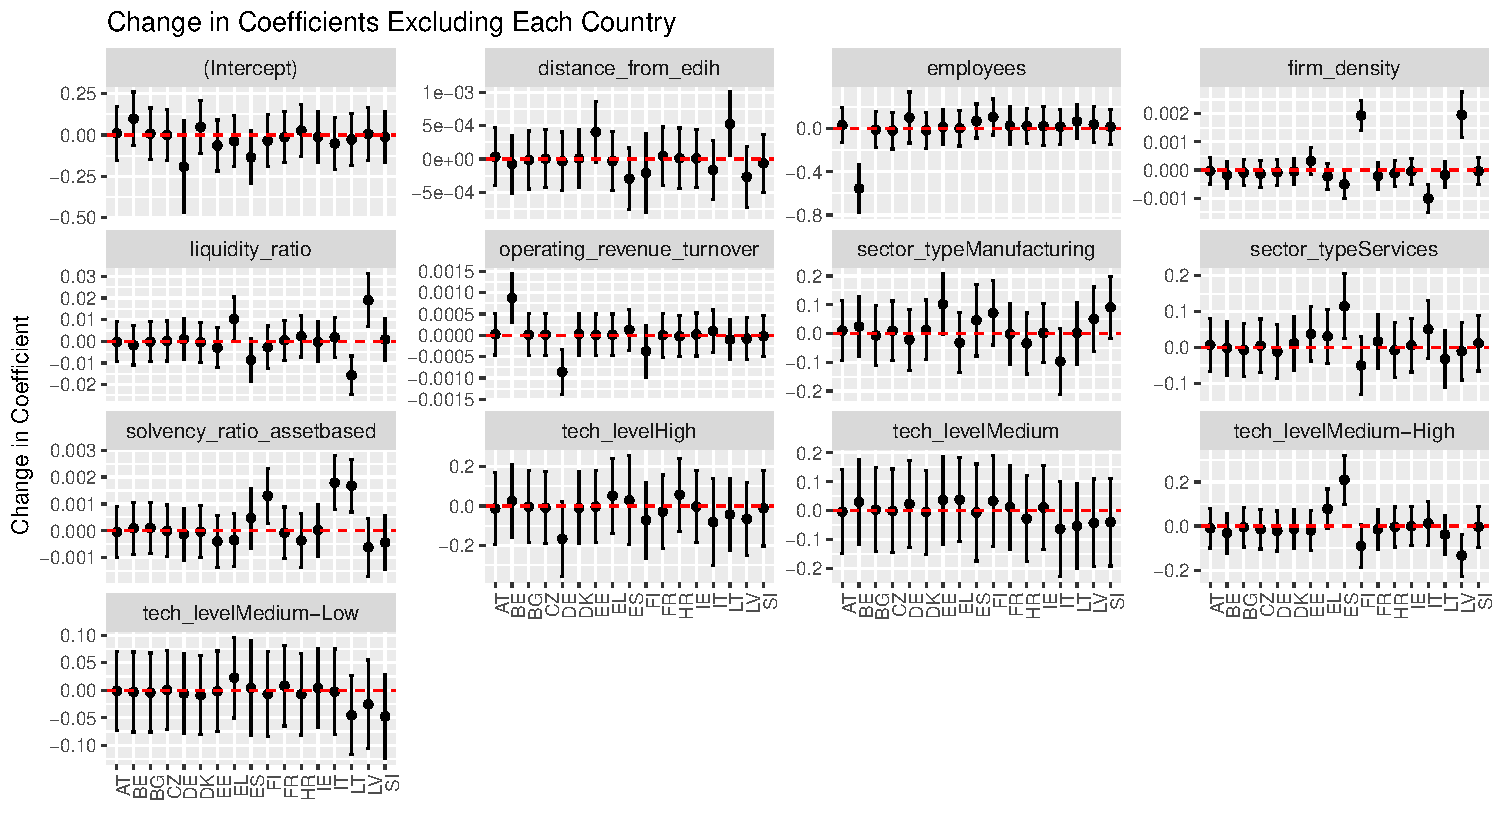
\includegraphics[width=\textwidth]{../Output/changes-in-coeff-nocountryeffects-LEGACY.pdf}
    \caption{\centering{Changes in coefficients caused by the exclusion of each country. Error bars are Standard Errors from the coefficient estimation.}}
    \label{fig:changes_in_coeff-nocountryeffects-BIGFORMAT}
\end{sidewaysfigure}



\par We can see here how for most of the coefficients the results are stable when removing one country at a time from the sample. However, if we focus on the coefficient for the Distance variable, we can see how the exclusion of Italy from the sample would lead to a slightly significant positive change of the coefficient. This is an indication that the negative effect of distance is stronger in the italian subsample of firms. However, even when accounting for the potential change, the coefficient for distance would remain negative and significant.

\par Moving on to Firm Density, it is clear that the exclusion of the Baltics, specifically Finland and Latvia, leads to a significant positive change in the coefficient. This suggests that the positive effect of firm density is actually weakened by the presence of firms in the Baltic States. This could be due to the specific geographical characteristics of the area, which is more sparsely populated than other regions of the EU. Consequently, most firms in the sample are concentrated in small pockets of high firm density, reducing the variability needed to accurately estimate the coefficient and thus pushing it towards zero. Other countries which when excluded move the coefficient are Italy and (to a lesser degree) Spain, both moving the coefficient in the negative direction when excluded, meaning their inclusion is having a positive effect on the coefficient. This can be due to a multiplicity of reasons, however one probable cause is the fact that both Italy and Spain have a very good coverage of the population of firms in ORBIS. Thus, even "rural" firms are included in the control group, and since instead most of the treated firms come from high-firm-density areas, the coefficient is pushed upwards.

\par Focusing on the firm-level characteristics, we can see how the coefficient of the Employees variable seems to be driven by Belgium. When excluding the small country, the coefficient drops significantly. One potential reason for this could be that most of the very large firms in the treated sample come from Belgium, thus increasing the effect of firms' size in the subsample. For the Liquidity Ratio, the coefficient is driven by the exclusion of Italy and Latvia: Italy when excluded drops the coefficient, while Latvia increases it. However, none of the two would change the significance or sign of the coefficient. For the Turnover variable, the coefficient is once again influenced by Belgium, as well as Germany. Since the coefficient in the analysis was not significant, this could mean that these two countries were the ones making the coefficient closer to zero. Once we exclude one or the other, the coefficient shifts enough to be considered significant. The Solvency Ratio coefficient is lifted upwards by the exclusion of Finland, Italy and Lithuania. However, this is going in the same direction of the sign of the coefficient, thus not changing the interpretation of the results.

\par With regards to the sectoral variables, most of their coefficients stay put, apart from Services when excluding Spain, which increases the coefficient. This is paralleled in the tech level coefficients, where we can see that they stay unchanged everywhere, apart from the Medium-High tech level when excluding Spanish firms, which increases the coefficient. This could indicate that the positive effect of being in the Services sector and in a medium-high tech level segment is significantly weaker in Spain than in the other countries present in the subsample. Again, however, the potential coefficient change would not alter the interpretation of the results from the regression.

\par In summary, the regression results show us what the key drivers of participation in the EDIH initiative are. Proximity to EDIH hubs and higher firm density are significant spatial factors influencing participation. Additionally, firms in the Manufacturing and Services sectors, as well as those in technologically intensive sectors, are more likely to engage with the initiative. Larger firms and those with higher solvency ratios also show a higher propensity to participate. These findings are for the most part consistent across different sectors and countries, as shown by the sectorial regression and by the analysis of changes in the coefficients when excluding each country from the sample.




\newpage
\chapter{Discussion and Conclusions}

\par As discussed in the previous chapter, the results of the analysis allows us to answer to our main research question, on the identification of the drivers of firms' participation to the EDIH initiative. As the regression results show, geospatial characteristics do have a role to play in the propensity of firms to participate in the initiative. In particular, firms that are located closer to EDIH hubs are more likely to take part in the initiative, and firms that are located in areas with high firm density are also more likely to participate. Moreover, sectoral characteristics also play a role, with the Manufacturing sector being more likely to participate, and more technologically intensive sectors being on average more likely to get involved in the initiative. Firm-level characteristics also play a role, especially size (number of employees) and financial constraint metrics.
\par How does the EDIH program fare so far then? The results of the analysis suggest that the initiative is effectively targeting firms that are in need of digitalization support, as evidenced by the fact that the coefficient related to the liquidity ratio is negative. On the other hand, the program seems to attract larger firms, and those with higher solvency ratios. This could be a sign that the initiative is not reaching the smallest firms. However, it can be argued that micro-firms may see less of an incentive in participating in the program, and probably face more barriers to participation, such as lack of resources or lack of awareness of the initiative. This should not be seen as an outright failure on the part of the EDIH program, since it is also possible that a minimum level of resources is needed to engage with the initiative effectively. Furthermore, the initiative is designed to kickstart the catching-up progress of the European economy, which is more likely to come from small and medium enterprises than from micro firms with 1 or 2 employees. Regarding the positivity of the coefficient for the solvency ratio instead, as we briefly touched in the previous chapter, it can be a good sign of the fact that the EDIH initiative is not an outright subsidy for inefficient firms on the brink of bankruptcy, but rather a policy attracting firms in good financial health, albeit not as rich in liquidity as to be financially unconstrained. In fact, the liquidity ratio measures the short-term ability of the firm to pay its debts, while the solvency ratio indicates the long-term financial stability of the company. Thus the fact that the initiative is attracting firms with higher solvency ratios means that the firms are likely to survive in the long term, indicating that the public investment in the initative is likely to be well spent.
\par The positive effects related to sectors with higher technological intensity are also good news, meaning that the impact of the policy is likely going to be stronger, since those are specifically the sectors in which the European economy needs to catch up.
\par Regarding the country-group dummies instead, they show the importance of EDIH's internal expertise, since it is clear how those regions that already had a strong experience with the DIH initiative experienced faster kickstart of the EDIH initiative itself, probably because they were already well-equipped to start at full speed. If this interpretation is correct, we should see this effect attenuate in the future, as (hopefully) the other regions catch up in terms of expertise and experience.
\par The coefficients related to geospatial characteristics instead stress the necessity of a good coverage of the whole EU territory for the initiative. These results can serve as an indication to policymakers needing to decide where to place potential additional EDIHs. Knowing that distance from the hub serves as a potential barrier to participation, adding offices in areas where no hubs are present could be a good strategy to increase the reach of the initiative.
\par Let's not forget however that the analysis performed presents some limitations and drawbacks, which prevent us from having a more clear picture of the effectiveness of the initiative and providing more insights and advice on how to make it better.
\par For instance, the analysis is based on a sample of control-group firms that may or may not be representative of the overall population of firms in the EU. As said in the previous chapter when describing how the control group was constructed, the ORBIS database does not have equally good coverage in all EU countries, and this could have introduced a bias in the results. Furthermore, for both the treated and the control group, it is possible that availability of data for the variables that were included in the analysis is indeed correlated with the probability to access the EDIH initiative. As an example, if the ORBIS database is more likely to have data on older firms, and for some reason age of the firm has a positive impact on the propensity to participate in the EDIH initiative, then we would have a problem, since we would have a positive bias in the results. The reason for that is the way the matching process is present for treated firms but not for the control group, leading to the possibility of the matched subsample of the treated group potentially being not representative of the overall treated group. This limitation would be challenging to overcome, since even if we already know which variables are correlated with a better coverage in ORBIS, we do not know \textit{a priori} what their effect on the probability to participate in the EDIH initiative is.
\par There are of course also ways to improve the analysis, as well as avenues for future research on the topic. For example, even while still keeping the same methodology, it would be interesting to check if there are any word-of-mouth effects, meaning that being close to a firm that is already participating in the initiative could increase the probability of a firm to participate as well. This could be done by adding a variable that counts the number of treated firms in a certain radius around the firm, similar to how firm density was computed. Another interesting future research question would be on the proper functioning of the network of hubs itself, meaning whether hubs do in fact operate as a network, by exchanging clients, or if they act mostly on their own. In that case the analysis would have to be done on an EDIH basis, and not on an individual firm basis. 
\par Of course, when more data will be available down the line, regarding $T1$ observations and eventually $T2$ observations, it will be possible to perform a more robust analysis, with a difference-in-differences approach, to see if the EDIH initiative is indeed effective. However, the efffectiveness check cannot be done on the Digital Maturity score itself, since the DMA was never sent to a control group of firms. The DMA can eventually be used to see if the adoption of targeted technologies increases in the treated group, but having no possible comparison makes it tricky to attribute the potential increase to the EDIH initiative, as opposed to some other factor.
What will be possible however is to check the effectiveness of the initiative in having a positive impact on firm-level characteristics in the medium-term. Any effect on outcomes such as profitability of the firm, its size, or its financial health, would be a good indication of the effectiveness of the initiative. Even if not directly proving efficacy in providing digitalization, an increase in those metrics in the treated group vis-a-vis the control group would indicate the success of the initiative in supporting the catching-up process the European economy needs to become competitive again on the global stage.
\par Overall, to conclude we can say that the initial indication is that the program is going in the right direction, seemingly targeting the right demographic group of firms to increase its probability of success in the future. The size and sign of the coefficients related to geospatial characteristics indicate the need to maintain a network of EDIHs with a good coverage of the entire EU territory. Time (and upcoming data from the DMA) will tell us if the initiative is indeed effective in supporting the digitalization of the European economy, and if it will be ultimately successful triggering the improvement in firm's outcomes that the European Commission is hoping for. 




\newpage
\appendix
\chapter{Additional Tables and Figures}

% Large countries
\begin{figure}[ht]
    \centering
    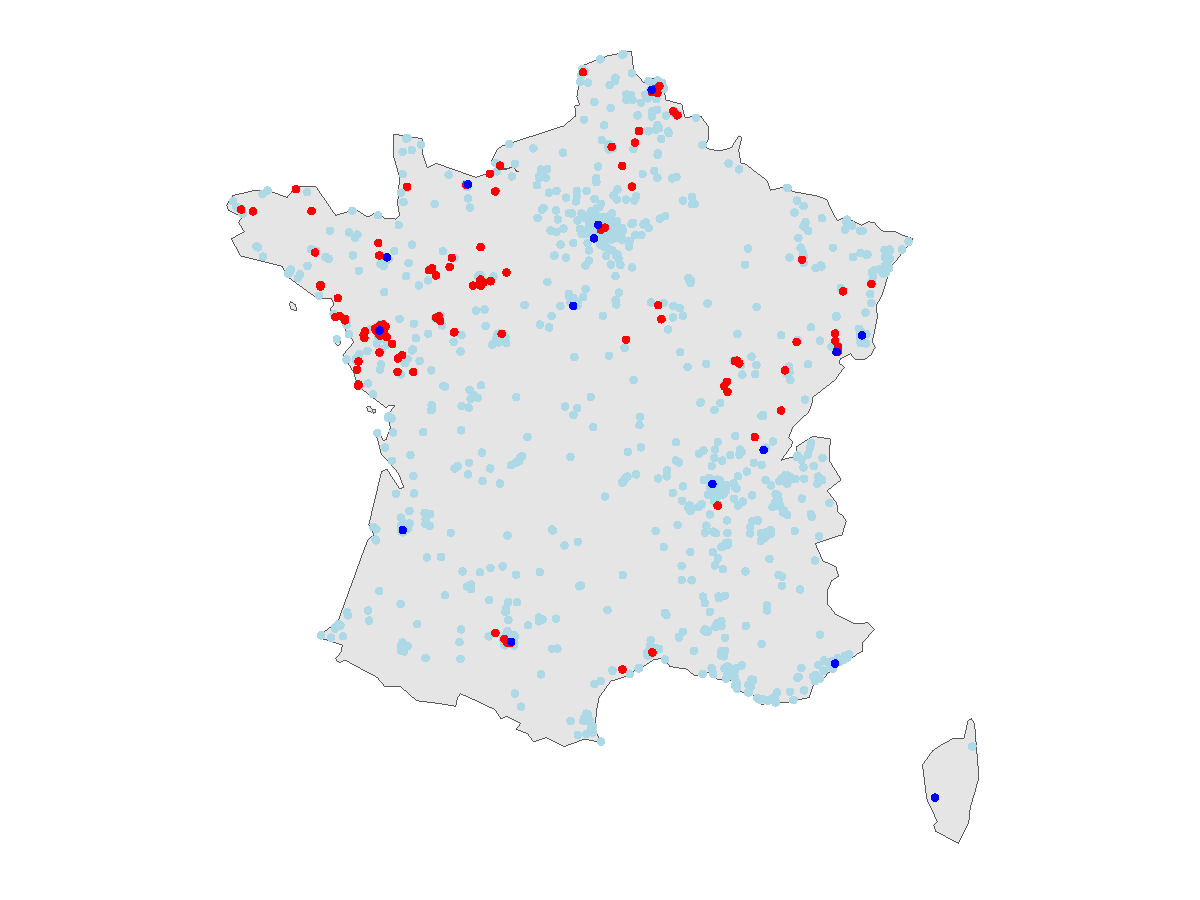
\includegraphics[width=0.62\textheight,trim={2cm 0cm 2cm 0cm},clip]{../Output/FR_map.pdf}
    \caption{France}
    \label{fig:map_obs_FR}
\end{figure}

\newpage
\begin{figure}[ht]
    \centering
    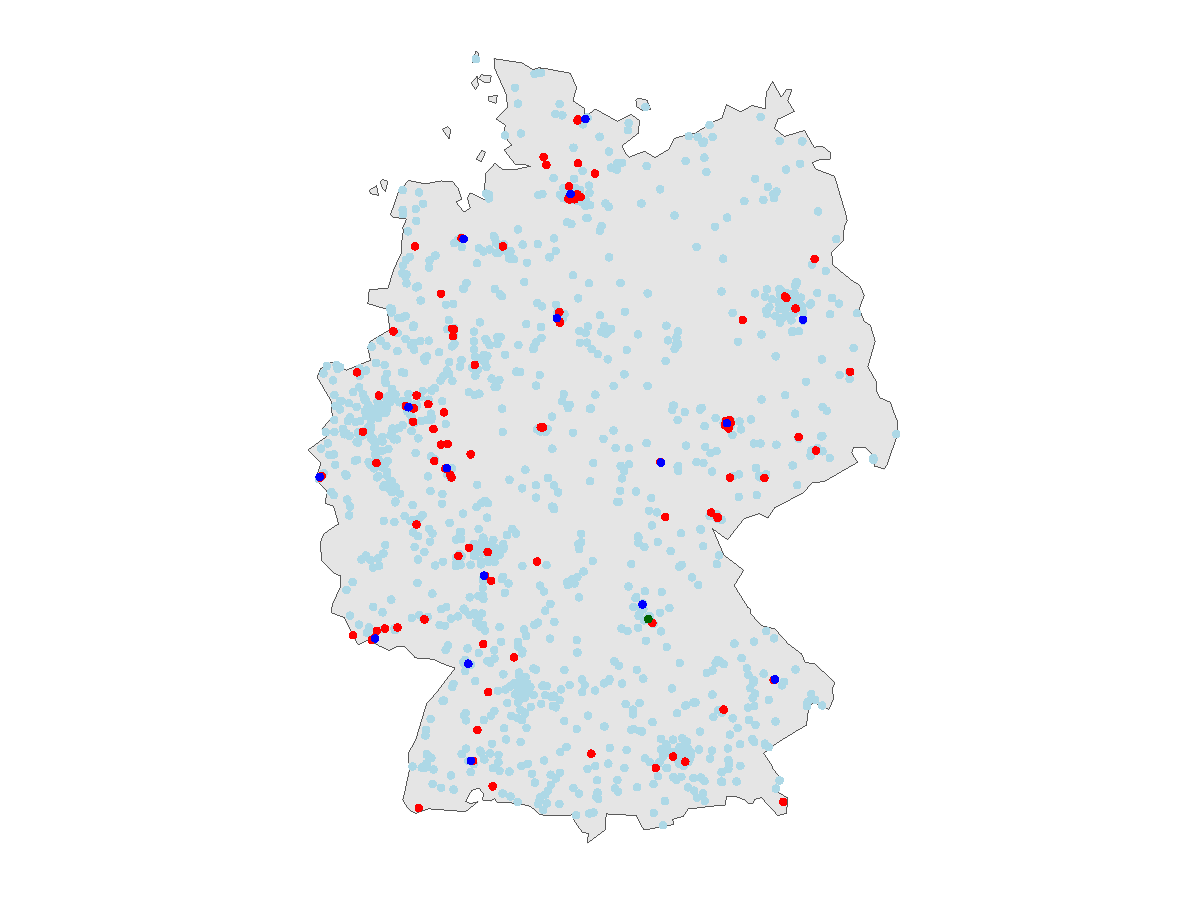
\includegraphics[width=.9\textheight,trim={3cm 0cm 2.5cm 0.5cm},clip]{../Output/DE_map.pdf}
    \caption{Germany}
    \label{fig:map_obs_DE}
\end{figure}

\newpage
\begin{sidewaysfigure}[p]
    \centering
    \includegraphics[width=.95\textheight,trim={0cm 0cm 0cm 0.5cm},clip]{../Output/ES_map.pdf}
    \caption{Spain}
    \label{fig:map_obs_ES}
\end{sidewaysfigure}

\newpage
\begin{figure}[ht]
    \centering
    \includegraphics[width=.9\textheight,trim={2.8cm 0cm 2.5cm 0.5cm},clip]{../Output/IT_map.pdf}
    \caption{Italy}
    \label{fig:map_obs_IT_1}
\end{figure}


% Small countries
\begin{figure}[ht]
    \centering
    \begin{subfigure}[b]{0.45\textwidth}
        \centering
        \includegraphics[width=\linewidth]{../Output/AT_map.pdf}
        \caption{Austria}
        \label{fig:map_obs_AT}
    \end{subfigure}
    \hfill
    \begin{subfigure}[b]{0.45\textwidth}
        \centering
        \includegraphics[width=\linewidth]{../Output/BE_map.pdf}
        \caption{Belgium}
        \label{fig:map_obs_BE}
    \end{subfigure}
    \vfill
    \begin{subfigure}[b]{0.45\textwidth}
        \centering
        \includegraphics[width=\linewidth]{../Output/BG_map.pdf}
        \caption{Bulgaria}
        \label{fig:map_obs_BG}
    \end{subfigure}
    \hfill
    \begin{subfigure}[b]{0.45\textwidth}
        \centering
        \includegraphics[width=\linewidth]{../Output/CZ_map.pdf}
        \caption{Czech Republic}
        \label{fig:map_obs_CZ}
    \end{subfigure}
    \vfill
    \begin{subfigure}[b]{0.45\textwidth}
        \centering
        \includegraphics[width=\linewidth]{../Output/DK_map.pdf}
        \caption{Denmark}
        \label{fig:map_obs_DK}
    \end{subfigure}
    \hfill
    \begin{subfigure}[b]{0.45\textwidth}
        \centering
        \includegraphics[width=\linewidth]{../Output/EE_map.pdf}
        \caption{Estonia}
        \label{fig:map_obs_EE}
    \end{subfigure}
\end{figure}

\begin{figure}[ht]
    \centering
    \begin{subfigure}[b]{0.45\textwidth}
        \centering
        \includegraphics[width=\linewidth]{../Output/SI_map.pdf}
        \caption{Slovenia}
        \label{fig:map_obs_SI}
    \end{subfigure}
    \hfill
    \begin{subfigure}[b]{0.45\textwidth}
        \centering
        \includegraphics[width=\linewidth]{../Output/EL_map.pdf}
        \caption{Greece}
        \label{fig:map_obs_EL}
    \end{subfigure}
    \vfill
    \begin{subfigure}[b]{0.45\textwidth}
        \centering
        \includegraphics[width=\linewidth]{../Output/HR_map.pdf}
        \caption{Croatia}
        \label{fig:map_obs_HR}
    \end{subfigure}
    \hfill
    \begin{subfigure}[b]{0.45\textwidth}
        \centering
        \includegraphics[width=\linewidth]{../Output/IE_map.pdf}
        \caption{Ireland}
        \label{fig:map_obs_IE}
    \end{subfigure}
    \vfill
    \begin{subfigure}[b]{0.45\textwidth}
        \centering
        \includegraphics[width=\linewidth]{../Output/LT_map.pdf}
        \caption{Lithuania}
        \label{fig:map_obs_LT}
    \end{subfigure}
    \hfill
    \begin{subfigure}[b]{0.45\textwidth}
        \centering
        \includegraphics[width=\linewidth]{../Output/LV_map.pdf}
        \caption{Latvia}
        \label{fig:map_obs_LV}
    \end{subfigure}
\end{figure}

\begin{figure}[ht]
    \centering
    \begin{subfigure}[b]{0.5\textwidth}
        \centering
        \includegraphics[width=0.5\textheight]{../Output/NL_map.pdf}
        \caption{Netherlands}
        \label{fig:map_obs_NL}
    \end{subfigure}
    
    \vspace{1cm}
    
    \begin{subfigure}[b]{0.5\textwidth}
        \centering
        \includegraphics[width=0.5\textheight]{../Output/FI_map.pdf}
        \caption{Finland}  
        \label{fig:map_obs_FI}
    \end{subfigure}
\end{figure}

% \begin{sidewaysfigure}[p]
%     \centering
%     \includegraphics[width=\textwidth]{../Output/changes-in-coeff-nocountryeffects.pdf}
%     \caption{\centering{Changes in coefficients caused by the exclusion of each country. Error bars are Standard Errors from the coefficient estimation.}}
%     \label{fig:changes_in_coeff-nocountryeffects-BIGFORMAT}
% \end{sidewaysfigure}

\begin{sidewaysfigure}[p]
    \centering
    \begin{subfigure}[b]{0.8\textwidth}
        \centering
        \includegraphics[width=\linewidth]{../Output/q1collapsed.png}
        \caption{Question 1: Digitalization Strategy}
    \end{subfigure}
    \vfill
    \begin{subfigure}[b]{0.8\textwidth}
        \centering
        \includegraphics[width=\linewidth]{../Output/q2.png}
        \caption{Question 2: Digital Transformation Readiness}
    \end{subfigure}
    \caption{Responses for Digital Business Strategy dimension}
\end{sidewaysfigure}

\begin{sidewaysfigure}[p]
    \centering
    \begin{subfigure}[b]{0.8\textwidth}
        \centering
        \includegraphics[width=\linewidth]{../Output/q3.png}
        \caption{Question 3: Basic Digital Technologies}
    \end{subfigure}
    \vfill
    \begin{subfigure}[b]{0.8\textwidth}
        \centering
        \includegraphics[width=\linewidth]{../Output/q4.png}
        \caption{Question 4: Advanced Digital Technologies}
    \end{subfigure}
    \caption{Responses for Digital Readiness dimension}
\end{sidewaysfigure}

\begin{sidewaysfigure}[p]
    \centering
    \begin{subfigure}[b]{0.8\textwidth}
        \centering
        \includegraphics[width=\linewidth]{../Output/q5.png}
        \caption{Question 5: Digital Skills}
    \end{subfigure}
    \vfill
    \begin{subfigure}[b]{0.8\textwidth}
        \centering
        \includegraphics[width=\linewidth]{../Output/q6.png}
        \caption{Question 6: Working Conditions}
    \end{subfigure}
    \caption{Responses for Human-Centric Digitalization dimension}
\end{sidewaysfigure}

\begin{sidewaysfigure}[p]
    \centering
    \begin{subfigure}[b]{0.8\textwidth}
        \centering
        \includegraphics[width=\linewidth]{../Output/q7.png}
        \caption{Question 7: Data Management}
    \end{subfigure}
    \vfill
    \begin{subfigure}[b]{0.8\textwidth}
        \centering
        \includegraphics[width=\linewidth]{../Output/q8.png}
        \caption{Question 8: Cybersecurity}
    \end{subfigure}
    \caption{Responses for Data Management dimension}
\end{sidewaysfigure}

\begin{sidewaysfigure}[p]
    \centering
    \includegraphics[width=0.8\textwidth]{../Output/q9.png}
    \caption{Question 9: Automation \& AI (Automation \& Intelligence dimension)}
\end{sidewaysfigure}

\begin{sidewaysfigure}[p]
    \centering
    \begin{subfigure}[b]{0.8\textwidth}
        \centering
        \includegraphics[width=\linewidth]{../Output/q10.png}
        \caption{Question 10: Environmental Sustainability}
    \end{subfigure}
    \vfill
    \begin{subfigure}[b]{0.8\textwidth}
        \centering
        \includegraphics[width=\linewidth]{../Output/q11.png}
        \caption{Question 11: Digital-Enabled Sustainable Processes}
    \end{subfigure}
    \caption{Responses for Green Digitalization dimension}
\end{sidewaysfigure}

\nocite{*}
\printbibliography




\end{document}
